\documentclass[11pt,a4paper,twoside]{book}

\usepackage{graphicx}
\usepackage[utf8]{inputenc}
\usepackage[spanish,activeacute,es-tabla]{babel}
\usepackage[left=3cm,right=3cm,bottom=3.5cm,top=3.5cm]{geometry}
\usepackage{euler}			% Texto matematico estilo Concrete Mathematics
\usepackage{color}		
\usepackage{amsthm}
\usepackage{amsmath}
\usepackage{amssymb}
\usepackage{hyperref}
\usepackage{wrapfig}
\usepackage[font=small,labelfont=bf]{caption}

\usepackage{algpseudocode}
\let\oldReturn\Return
\renewcommand{\Return}{\State\oldReturn}
\usepackage{algorithm}
\floatname{algorithm}{Algoritmo}
\renewcommand{\algorithmicrequire}{\textbf{Entrada:}}
\renewcommand{\algorithmicensure}{\textbf{Salida:}}

\algdef{SE}[FUNCTION]{Function}{EndFunction}%
   [2]{\textproc{ #1}(#2)}%\ifthenelse{\equal{#2}{}}{}{(#2)}}%
   {\algorithmicend\ \algorithmicfunction}%
\algtext*{EndFunction}
\algtext*{EndIf}
\algtext*{EndFor}
\algtext*{EndWhile}

\algnewcommand\algorithmicforeach{\textbf{for each}}
\algdef{S}[FOR]{ForEach}[1]{\algorithmicforeach\ #1\ \algorithmicdo}

\graphicspath{{img/}}

\renewcommand{\And}{\textbf{and} }
\newcommand{\Or}{\textbf{or} }
\newcommand{\True}{\textbf{true} }
\newcommand{\False}{\textbf{false} }
\newcommand{\Break}{\textbf{break} }

\newcommand{\todo}[1]{{\noindent \Large \color{red}TO-DO: \textbf{#1}}}
\newcommand{\problem}[1]{\textnormal{\textsf{#1}}}
\newcommand{\dist}{\textnormal{dist}}
\newcommand{\distmax}{\overline{\textnormal{dist}}}
\newcommand{\length}{\textnormal{length}}
\newcommand{\weight}{\textnormal{weight}}
\newcommand{\ceil}[1]{\left\lceil #1 \right\rceil}
\newcommand{\floor}[1]{\left\lfloor #1 \right\rfloor}
\newcommand{\mst}{\textnormal{MST}}
\newcommand{\class}[1]{\textnormal{\textbf{#1}}}
\newcommand{\poly}{\textnormal{poly}}
\newcommand{\prev}{\textnormal{prev}}
\newcommand{\cov}{\textnormal{cov}}
\newcommand{\startsr}{\texttt{Start-SR}}
%\newcommand{\eendsr}{\texttt{End-SR}}
\newcommand{\toursr}{\texttt{Tour-SR}}
\newcommand{\throughsr}{\texttt{Through-SR}}
\newcommand{\sr}{\texttt{SR}}
\newcommand{\clients}{\texttt{X}}
\newcommand{\val}{\textnormal{val}}
\newcommand{\size}{\textnormal{size}}

\newtheorem{theorem}{Teorema}[chapter]
\newtheorem{lemma}{Lema}[chapter]
\newtheorem{corollary}{Corolario}[chapter]
\newtheorem{claim}{Afirmaci\'on}[chapter]
\newtheorem{proposition}{Proposici\'on}[chapter]
\theoremstyle{definition}
\newtheorem{definition}{Definici\'on}[chapter]
\newtheorem{remark}{Observaci\'on}[chapter]

%\newcommand{\theoremautorefname}{Teorema}
\newcommand{\lemmaautorefname}{Lema}
\newcommand{\corollaryautorefname}{Corolario}
\newcommand{\claimautorefname}{Afirmaci\'on}
\newcommand{\propositionautorefname}{Proposici\'on}
\newcommand{\definitionautorefname}{Definici\'on}
\newcommand{\remarkautorefname}{Observaci\'on}
\newcommand{\algorithmautorefname}{Algoritmo}

% Macro para escribir problemas.
\newcommand{\decpr}[3]{
%     \decpr{NAME}{INSTANCE}{QUESTION}
\begin{list}{}{
\setlength{\leftmargin}{0.1in}
\setlength{\rightmargin}{0.1in}
\setlength{\parsep}{0pt}
\setlength{\itemsep}{2pt}
\setlength{\topsep}{\itemsep}
\setlength{\partopsep}{\itemsep}
}
\item
{\problem{#1}}
\item
{INSTANCIA: #2}
\item
{SALIDA: #3}
\end{list}
\vspace{1mm}
}

\newcommand{\optpr}[3]{
%     \optpr{NAME}{INSTANCE}{QUESTION}

\begin{list}{}{
\setlength{\leftmargin}{0.1in}
\setlength{\rightmargin}{0.1in}
\setlength{\parsep}{0pt}
\setlength{\itemsep}{2pt}
\setlength{\topsep}{\itemsep}
\setlength{\partopsep}{\itemsep}
}
\item
{\problem{#1}}
\item
{INSTANCIA: #2}
\item
{SALIDA: #3}
\end{list}
\vspace{1mm}
}

% Fuente estilo Concrete Mathematics.
%\renewcommand{\rmdefault}{pplx}

% Configuracion de hyperref
\hypersetup{colorlinks=true,linkcolor=blue,citecolor=blue}

\begin{document}

%%%% CARATULA
\def\titulo{Licenciado }

\def\autor{Guido Tagliavini Ponce}
\def\tituloTesis{Star Routing: Entre Ruteo de Veh'iculos y Vertex Cover}
\def\runtitulo{Star Routing: Entre Ruteo de Veh'iculos y Vertex Cover}
\def\runtitle{Star Routing: Between Vehicle Routing and Vertex Cover}
\def\director{Diego Delle Donne}
\def\codirector{Javier Marenco}
\def\lugar{Buenos Aires, 2017}
\newcommand{\HRule}{\rule{\linewidth}{0.2mm}}
%
\thispagestyle{empty}

\begin{center}\leavevmode

\vspace{-2cm}

\begin{tabular}{l}

\includegraphics[width=2.6cm]{img/logofcen.pdf}
\end{tabular}


{\large \sc Universidad de Buenos Aires

Facultad de Ciencias Exactas y Naturales

Departamento de Computaci\'on}

\vspace{6.0cm}

%\vspace{3.0cm}
%{
%\Large \color{red}
%\begin{tabular}{|p{2cm}cp{2cm}|}
%\hline
%& Pre-Final Version: \today &\\
%\hline
%\end{tabular}
%}
%\vspace{2.5cm}

{\huge\bf \tituloTesis}

\vspace{2cm}

{\large Tesis presentada para optar al t\'{\i}tulo de\\
\titulo en Ciencias de la Computaci\'on}

\vspace{2cm}

{\Large \autor}

\end{center}

\vfill

{\large

{Director: \director}

\vspace{.2cm}

{Codirector: \codirector}

\vspace{.2cm}

\lugar
}

\newpage\thispagestyle{empty}


%%%% ABSTRACTS, AGRADECIMIENTOS Y DEDICATORIA
\frontmatter
\pagestyle{empty}
%\begin{center}
%\large \bf \runtitulo
%\end{center}
%\vspace{1cm}
\chapter*{\runtitulo}

En esta tesis consideramos el problema \problem{STAR ROUTING} (abreviado \problem{SR}) que toma un grafo simple y no dirigido $G$ y un subconjunto de aristas $X$, y pide encontrar un camino $P$ de $G$ tal que toda arista de $X$ tiene al menos un extremo en $P$, de longitud m'inima.

Estudiamos la complejidad computacional del problema. Probamos que el problema es \class{NP-completo} en el caso general, restringido a grafos grillas (asumiendo una representaci'on no est'andar de $G$) y restringido a grafos completos. Probamos que en el caso de los 'arboles el problema est'a en \class{P} y damos un algoritmo de tiempo lineal que lo resuelve en ese caso.

Exhibimos dos algoritmos exactos junto con heur'isticas para acelerar el c'omputo. La importancia de estos algoritmos es principalmente te'orica, pues los resultados experimentales muestran que no son suficientemente r'apidos como para resolver instancias de tama\~no real, en una cantidad de tiempo razonable.

Exhibimos algoritmos aproximados para el problema en su versi'on general, y restringido a grillas y a grafos completos. En particular, concluimos que el caso general se puede aproximar por un factor constante del 'optimo. Para grafos grilla damos un algoritmo $(9/2)$-aproximado, y para grafos completos damos, para todo $\varepsilon > 0$, un algoritmo $(2 + \varepsilon)$-aproximado.\\

Adem'as de estudiar el problema \problem{SR}, consideramos un problema asociado denominado \problem{STOPS SELECTION} (abreviado \problem{SS}), que toma una instancia $(G, X)$ de \problem{SR} y un camino $P$ que es soluci'on factible de \problem{SR} para $(G, X)$, y pide encontrar un m'inimo subconjunto $S$ de v'ertices de $P$ tal que toda arista de $X$ tiene al menos un extremo en $S$. Probamos que este problema es \class{NP-completo} en el caso general. Damos un algoritmo exacto, que resulta ser polinomial para grafos bipartitos. Damos adem'as un algoritmo $2$-aproximado. Tanto el algoritmo exacto como el algoritmo aproximado son reducciones al problema de vertex cover m'inimo.\\

Hasta donde sabemos, ni el problema \problem{SR} ni el problema \problem{SS} han sido estudiados en la literatura previamente.

\bigskip

\noindent\textbf{Palabras claves:} ruteo de veh'iculos, vertex cover, complejidad computacional, algoritmos exactos, algoritmos aproximados.

\cleardoublepage
%\begin{center}
%\large \bf \runtitle
%\end{center}
%\vspace{1cm}
\chapter*{\runtitle}

In this thesis we consider the \problem{STAR ROUTING} problem (abbreviated as \problem{SR}) which takes a simple undirected graph $G$ and a subset of edges $X$, and asks to find a path $P$ of $G$ such that every edge in $X$ has at least one endpoint in $P$, with minimum length.

We study the problem's computational complexity. We prove the problem is \class{NP-complete} in the general case, restricted to grid graphs (assuming a non-standard representation for $G$) and restricted to complete graphs. We prove that for trees the problem is in \class{P} and we give a linear-time algorithm that solves it in that case.

We give two exact algorithms along with heuristics to speed up the computation. The importance of these algorithms is mainly theoretical, since experimental results show they are not fast enough to solve real-life instances, in a reasonable amount of time.

We give approximation algorithms for the problem in the general case, and restricted to grid and complete graphs. In particular, we conclude the general case can be approximated within a constant factor of the optimal. For grid graphs we give a $(9/2)$-approximation algorithm, and for complete graphs we give, for all $\varepsilon > 0$, a $(2 + \varepsilon)$-approximation algorithm.\\

Besides studying the \problem{SR} problem, we consider a related problem called \problem{STOPS SELECTION} (abbreviated as \problem{SS}), which takes an instance $(G, X)$ of \problem{SR} and a path $P$ that is a feasible solution of \problem{SR} for $(G, X)$, and asks to find a minimum subset $S$ of vertices of $P$ such that every edge in $X$ has at least one endpoint in $S$. We prove this problem is \class{NP-complete} in the general case. We give an exact algorithm, that turns out to be polynomial for bipartite graphs. We also give a $2$-approximation algorithm. Both the exact algorithm and the approximation algorithm are reductions to the minimum vertex cover problem.\\

To the best of our knowledge, neither the \problem{SR} problem nor the \problem{SS} problem have been studied in the literature.

\bigskip

\noindent\textbf{Keywords:} vehicle routing, vertex cover, computational complexity, exact algorithms, approximation algorithms.

\cleardoublepage
\chapter*{Agradecimientos}


\cleardoublepage
\tableofcontents

\mainmatter
\pagestyle{headings}

\chapter{Introducci'on}

\section{Los problemas}

Supongamos que estamos a cargo de la distribuci'on de la edici'on f'isica de un importante diario en una gran ciudad, para clientes suscriptos. Las entregas se hacen al domicilio de cada cliente, utilizando camiones de reparto, como el que se muestra en la \autoref{fig:boston}. Estos camiones circulan por la ciudad, recorriendo, uno por uno, los domicilios a los que se debe hacer una entrega.

\begin{wrapfigure}{r}{0cm}
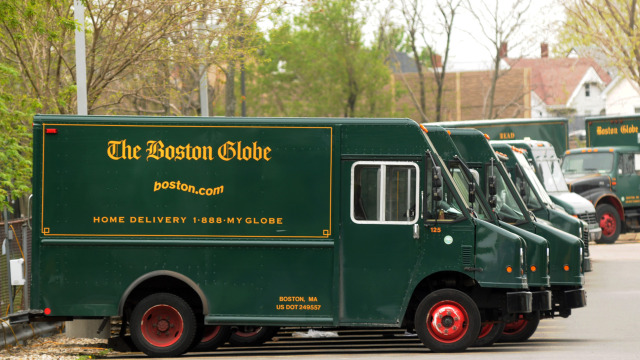
\includegraphics[scale=1.4]{img/boston.jpg}
\caption{Cami'on de reparto del diario \textit{The Boston Globe}.}
\label{fig:boston}
\end{wrapfigure}

Durante el procedimiento de reparto usual, un cami'on se detiene en la puerta de un domicilio y el conductor desciende del mismo, retira tantos diarios como haya que entregar all'i, y hace entrega de los mismos. Luego, vuelve a subirse al cami'on, y conduce hacia la puerta del siguiente domicilio.

Una alternativa a esto es un sistema de reparto en el que un cami'on no se detiene en la puerta de cada domicilio, sino en las esquinas de las calles de los clientes. Al detenerse en una esquina, el conductor desciende del cami'on, y realiza las entregas a todos los clientes que est'an sobre cada una de las cuadras incidentes a esa esquina (que suelen ser 4), a pi'e. Este sistema reduce el recorrido realizado por el cami'on, y lo compensa con recorrido a pi'e. Por lo tanto, es especialmente conveniente cuando hay una alta densidad de tr'ansito vehicular. Tambi'en es potencialmente mejor que el sistema tradicional en zonas donde hay una alta concentraci'on de clientes, a'un si hay poco tr'ansito, porque permite  realizar varias entregas, haciendo una 'unica descarga de diarios del cami'on. Notar que este sistema puede ser utilizado en otros contextos que involucren el reparto de productos, como por ejemplo la distribuci'on de encomiendas y paquetes, que realizan empresas como FedEx o UPS.

Como en toda empresa, queremos optimizar costos. En particular, queremos minimizar el recorrido que hace un cami'on, para realizar todas sus entregas. Como un primer paso en el estudio de este problema, nos vamos a concentrar en el reparto que debe realizar un 'unico cami'on. El problema que queremos resolver toma un conjunto de domicilios en los que debemos entregar ejemplares del diario, busca calcular un camino que le permita realizar todas las entregas a un cami'on (utilizando el sistema de reparto de detenciones en las esquinas), que recorra la m'inima cantidad de cuadras posible.

Podemos modelar este problema con un grafo simple y no dirigido $G$, que representa la ciudad, y un subconjunto $X$ de aristas de $G$, que representa aquellas cuadras en las que est'an ubicados los clientes. A cada arista $e \in X$ la llamaremos \textit{cliente}. Si bien podr'ia ocurrir que haya varios clientes en una misma cuadra, en este trabajo s'olo nos importa la existencia o no de clientes, y no la cantidad, en una cuadra. El problema \problem{STAR ROUTING} (abreviado \problem{SR}) consiste en encontrar un camino de $G$, tal que cada cliente tiene alguno de sus extremos en el camino, de longitud m'inima. Esto es, el camino pasa, en alg'un momento, por alguno de los cruces adyacentes a la cuadra de cada uno de los domicilios. La \autoref{fig:introduccion_1} muestra tres soluciones factibles distintas para una instancia de \problem{SR}. En ese caso, el grafo de entrada es una grilla. Esta clase de instancias es de especial inter'es, pues permite modelar adecuadamente la topolog'ia de una ciudad.

\begin{figure}[h]
	\begin{center}
		\input{img/introduccion_1.pdf_tex}
	\end{center}		
	\caption{Soluciones factibles de \problem{SR}. (a) y (b) son 'optimas; (c) no es 'optima. Las aristas en rojo son clientes, y las flechas violetas indican la soluci'on.}
	\label{fig:introduccion_1}
\end{figure}

Si una soluci'on factible visita uno de los extremos de un cliente $e$, el cami'on de entrega podr'a, si as'i lo desea, detenerse en ese punto y realizar la entrega de productos a ese (y posiblemente otros) cliente. Sin embargo, una soluci'on de \problem{SR} no establece en qu'e esquinas debe detenerse el cami'on para realizar todas las entregas. Lo 'unico que nos garantiza, es que existe alguna forma de elegir las detenciones, que permita realizar todas las entregas. En particular, podr'iamos detenernos en cada esquina del camino, y entregar a todos los clientes restantes. Esta selecci'on de paradas podr'ia obligarnos a detener m'as veces de lo necesario, incrementando el tiempo total que insume el reparto, adem'as de aumentar el desgaste del cami'on, producto de las reiteradas puestas en marcha del mismo.

Esto motiva un problema asociado a \problem{SR}, que llamamos \problem{STOPS SELECTION} (abreviado \problem{SS}). Este problema toma una instancia de \problem{SR} y una soluci'on factible para la misma, encontrar un subconjunto de v'ertices del camino, tal que todo cliente tiene un extremo en el conjunto, de cardinal m'inimo. La \autoref{fig:introduccion_2} muestra tres soluciones factibles de \problem{SS} para la instancia de \problem{SR} de la \autoref{fig:introduccion_1}-(a).\\

\begin{figure}[h]
	\begin{center}
		\input{img/introduccion_2.pdf_tex}
	\end{center}		
	\caption{Soluciones factibles de \problem{SS}. (a) y (b) son 'optimas; (c) no es 'optima. Las circunferencias verdes indican la soluci'on.}
	\label{fig:introduccion_2}
\end{figure}

Los problemas \problem{SR} y \problem{SS} son el tema de estudio de este trabajo, aunque, como adelanta el t'itulo de la tesis, \problem{SR} es el objeto de estudio principal de la tesis, y es profundamente m'as complejo que \problem{SS}.

\section{Definiciones preliminares y notaci'on}

\subsection{M'etricas}

Sea $X$ un conjunto. Se dice que una funci'on $d: X \times X \to \mathbb{R}$ es una \textit{m'etrica} o \textit{distancia}, si para todo $a, b, c \in X$ cumple:

\begin{enumerate}
\item $d(a, b) \geq 0$ (no negatividad)
\item $d(a, b) = d(b, a)$ (simetr'ia)
\item $d(a, b) \leq d(a, c) + d(c, b)$ (desigualdad triangular)
\item $d(a, b) = 0$ si y s'olo si $a = b$.
\end{enumerate}

Sobre el plano eucl'ideo $\mathbb{R}^2$ se definen varias m'etricas frecuentemente utilizadas, dos de las cuales son la \textit{distancia Manhattan} y la \textit{distancia eucl'idea}. Si $p = (p_1, p_2), q = (q_1, q_2)$, la distancia Manhattan entre $p$ y $q$ es $d_1(p, q) := |p_1 - q_1| + |p_2 - q_2|$, y la distancia eucl'idea entre $p$ y $q$ es $d_2(p, q) := \sqrt{(p_1 - q_1)^2 + (p_2 - q_2)^2}$.

\subsection{Teor'ia de grafos}

Revisamos los conceptos fundamentales de teor'ia de grafos que usaremos a lo largo de la tesis. Un tratamiento extensivo sobre teor'ia de grafos b'asica puede encontrarse en \cite{Gr05}.

\subsubsection*{Grafos, adyacencias y grados}

Un \textit{grafo simple y no dirigido} es una tupla $G = (V, E)$, tal que $V$ es un conjunto finito de elementos llamados \textit{v'ertices}, y $E \subseteq \{\{u, v\}: u, v \in V, u \neq v\}$ es un conjunto de pares no ordenados de v'ertices, llamados \textit{aristas}. Es \textit{no dirigido} porque las aristas no tienen direcci'on, y \textit{simple} porque no hay m'ultiples aristas entre un mismo par de v'ertices, ni aristas con sus dos extremos en el mismo v'ertice. Para abreviar, diremos simplemente \textit{grafo}. En ocasiones, llamamos $V(G)$ y $E(G)$ a los conjuntos de v'ertices y aristas de $G$, respectivamente. Dada una arista $\{u, v\}$, sus \textit{extremos} son los v'ertices $u$ y $v$ que la componen.

En un grafo $G = (V, E)$, dos v'ertices $u, v \in V$ se dicen \textit{adyacentes} si $\{u, v\} \in E$. La \textit{vecindad} de un v'ertice $u \in V$ es el conjunto $N(u) = \{v \in V: u \text{ y } v \text{ son adyacentes}\}$. El \textit{grado} de un v'ertice $u \in V$ es $d(u) = |N(u)|$. Los grados de los v'ertices de un grafo cumplen el siguiente resultado, conocido como \textit{Handshake Lemma}.

\begin{lemma}
$\sum_{u \in V} d(u) = 2|E|$
\end{lemma}

\subsubsection*{Pesos}

Llamamos \textit{pesos} de un grafo $G = (V, E)$ a una funci'on $c: E \to \mathbb{Z}_{\geq 0}$. Por simplicidad, si $\{u, v\} \in E$, escribimos $c(u, v)$ 'o $c(v, u)$, en lugar de $c(\{u, v\})$. Una funci'on $c: V \times V \to \mathbb{R}$ que sea \emph{sim'etrica}, puede hacer las veces de pesos de $G$.

\subsubsection*{Caminos y circuitos}

Un \textit{camino} de un grafo es una secuencia $\langle u_1, \dots, u_r \rangle$ de v'ertices del grafo, tal que $u_i$ y $u_{i + 1}$ son adyacentes para todo $1 \leq i < r$. Un camino se dice \textit{simple} si no pasa m'as de una vez por cada v'ertice.

Un \textit{circuito} de un grafo es un camino que empieza y termina en el mismo v'ertice. Un circuito se dice \textit{simple} si contiene 3 o m'as v'ertices distintos, y no pasa m'as de una vez por cada uno, salvo por el v'ertice inicial y final.

Dado un camino o circuito $P$ de un grafo, la \textit{longitud de $P$}, notada $\length(P)$, es la cantidad de aristas de $P$. A la cantidad de v'ertices de $P$, visto como multiconjunto, la notamos $|P|$. Se tiene, por lo tanto, $\length(P) = |P| - 1$. Si la funci'on $c$ son los pesos del grafo, llamamos \textit{peso de $P$}, y lo notamos $\length_c(P)$, a la suma de los pesos, dados por $c$, de las aristas de $P$.

Un \textit{camino hamiltoniano} (resp. \textit{circuito hamiltoniano}) de un grafo, es un camino (resp. circuito) que pasa exactamente una vez por cada v'ertice del grafo. Un \textit{camino euleriano} (resp. \textit{circuito euleriano}) de un grafo, es un camino (resp. circuito) que pasa exactamente una vez por cada arista.

\subsubsection*{Grafos conexos y distancia}

Un grafo es \textit{conexo}, si para cada par de v'ertices del grafo existe un camino entre ellos.

Dado un grafo conexo $G$, la \textit{distancia} entre dos v'ertices $u$ y $v$ de $G$ es $\dist_G(u, v) := \min\{\length(P): P \text{ es un camino entre }u \text{ y }v \text{ en } G\}$. Cuando no haya ambig\"uedad sobre el grafo al que nos estamos refiriendo, escribiremos directamente $\dist(u, v)$. Notar que la distancia $\dist_G$ es una m'etrica, en el sentido matem'atico.

\subsubsection*{Subgrafos y subgrafos generadores}

Dado un grafo $G = (V, E)$, un \textit{subgrafo} de $G$ es un grafo $H = (V', E')$ tal que $V' \subseteq V$ y $E' \subseteq E$. Un \textit{subgrafo generador} de un grafo $G$ es un subgrafo $H$ tal que todo v'ertice de $G$ tambi'en es un v'ertice de $H$.

\subsubsection*{'Arboles y 'arboles generadores}

Un \textit{'arbol} es un grafo conexo sin circuitos simples. Un \textit{'arbol generador} es un subgrafo generador que adem'as es un 'arbol. Si $T$ es un 'arbol generador de un grafo $G$ con pesos $c$, notamos $\weight_c(T)$ a la suma de los pesos, dados por $c$, de las aristas de $T$. Un \textit{'arbol generador m'inimo} es un 'arbol generador que minimiza $\weight_c$, entre todos los 'arboles generadores del grafo. Notamos $\mst(G, c)$ al peso de un 'arbol generador m'inimo del grafo $G$ con pesos dados por $c$.

\subsubsection*{'Arboles con ra'iz}

Un \textit{'arbol con ra'iz} es un 'arbol en el que se ha distinguido un v'ertice, al que llamamos \textit{ra'iz}. Un 'arbol con ra'iz induce un ordenamiento jer'arquico de sus v'ertices, que es una clasificaci'on por nivel tal que los v'ertices del nivel $k$ son aquellos nodos a distancia $k$ de la ra'iz.

\subsubsection*{Subgrafos inducidos por aristas}

Dado un grafo $G = (V, E)$ y un subconjunto de aristas $F \subseteq E$, el subgrafo inducido de $G$ por $F$, notado $G[F]$, es el subgrafo de $G$ que contiene, exactamente, las aristas de $F$ y aquellos v'ertices que sean extremos de dichas aristas.

\subsubsection*{Grafos completos}

Un grafo es \textit{completo}, si todo par de v'ertices del grafo son adyacentes. 

Dado un conjunto finito $A$, notamos $K(A)$ al grafo completo que tiene como conjunto de v'ertices a $A$.

\subsubsection*{Grafos bipartitos}

Un grafo $G = (V, E)$ es \textit{bipartito}, si existe una partici'on $\{V_1, V_2\}$ de $V$, tal que toda arista de $G$ tiene un extremo en $V_1$ y otro en $V_2$.

\subsubsection*{Grafos grilla}

Un grafo es \textit{grilla}, si el conjunto de v'ertices y aristas de $G$ forman una grilla\footnote{Se puede definir grafo grilla en forma m'as rigurosa, como un producto cartesiano de grafos. A los fines de esta tesis, alcanza con una definici'on informal.}. En la \autoref{fig:introduccion_3} se exhibe un grafo grilla de $n$ v'ertices de alto por $m$ v'ertices de ancho. Observar que todo grafo grilla es un grafo bipartito. Una bipartici'on (la 'unica posible) se obtiene tomando los v'ertices por diagonales, en forma alternada.

\begin{figure}[h]
%\begin{wrapfigure}{r}{0cm}
\begin{center}
\input{img/introduccion_3.pdf_tex}
\caption{Un grafo grilla de $n$ filas y $m$ columnas.}
\label{fig:introduccion_3}
\end{center}
%\end{wrapfigure}
\end{figure}

\subsubsection*{Vertex covers y matchings}

Dado un grafo $G$, una arista $e$ de $G$ y un subconjunto $W$ de v'ertices (o un camino) de $G$, decimos que \textit{$W$ cubre a $e$} si $e$ tiene alg'un extremo en $W$.

Un \textit{vertex cover} de $G$ es un conjunto $S$ de v'ertices de $G$ tal que $S$ cubre a cada arista de $E$. Notamos $\tau(G)$ al m'inimo cardinal de un vertex cover de $G$.

Un \textit{matching} de $G$ es un conjunto $M$ de aristas de $G$ tal que no hay dos aristas de $M$ que tengan un extremo en com'un. Notamos $\nu(G)$ al m'aximo cardinal de un matching de $G$.

Estos dos conceptos est'an vinculados, como muestra el siguiente teorema.

\begin{theorem}
\label{th:nu_tau}
En todo grafo $G$, vale que el m'aximo cardinal de un matching de $G$ es menor o igual al m'inimo cardinal de un vertex cover de $G$. Esto es, $\nu(G) \leq \tau(G)$.

\begin{proof}
Sea $M = \{e_1, \dots, e_r\}$ un matching de $G$, y $S$ un vertex cover de $G$. Cada arista de $M$ debe ser cubierta por $S$, es decir que cada $e_i$ tiene al menos un extremo en $S$. Por ser $M$ un matching, sus aristas son disjuntas en sus extremos, dos a dos. Luego, $S$ contiene al menos $r = |M|$ v'ertices. Esto prueba que $|M| \leq |S|$, lo cual vale, en particular, si $M$ es m'aximo y $S$ es m'inimo.
\end{proof}
\end{theorem}
 
Una consecuencia de este teorema es que dado un grafo $G$, podemos dar una cota inferior de $\tau(G)$ exhibiendo un matching de $G$, y podemos dar una cota superior de $\nu(G)$ exhibiendo un vertex cover de $G$. En el caso de grafos bipartitos $\nu(G)$ y $\tau(G)$ coinciden, como prob'o K\H{o}nig en 1931.

\begin{theorem}[K\H{o}nig]
Si $G$ es un grafo bipartito, entonces $\tau(G) = \nu(G)$.
\end{theorem}

\subsection{Problemas de decisi'on y optimizaci'on}

Un \textit{problema de optimizaci'on} es aquel en el que cada instancia tiene asociada un conjunto $S$ de \textit{soluciones factibles}, cada una con un valor num'erico asociado, y el objetivo es encontrar una soluci'on factible cuyo valor sea \textit{'optimo} (m'inimo o m'aximo, seg'un el problema). Una soluci'on factible cuyo valor es 'optimo se denomina \textit{soluci'on 'optima}. El valor asociado a cada soluci'on est'a dado por una funci'on $\val: S \to \mathbb{R}$, llamada \textit{funci'on objetivo}. A modo de ejemplo, consideremos el famoso \problem{TRAVELING SALESMAN PROBLEM} (abreviado \problem{TSP}).

\optpr{TSP (optimizaci'on)}{$G = (V, E)$ un grafo completo y $c: E \to \mathbb{Z}_{\geq 0}$ los pesos de $G$.}{Un circuito hamiltoniano de $G$, de peso m'inimo.}

\noindent
En este caso, el conjunto de soluciones factibles es el de todos los circuitos hamiltonianos de $G$, y la funci'on objetivo es $\length_c$.

Si $I$ es una instancia de un problema de optimizaci'on $\Pi$, notamos $\Pi^*(I)$ al valor de la funci'on objetivo de una soluci'on 'optima. Cuando el contexto no de lugar a ambig\"uedad, notaremos $OPT = \Pi^*(I)$.\\

Un \textit{problema de decisi'on} es aquel en el que cada instancia s'olo tiene dos respuestas posibles: SI o NO. Retomando el ejemplo del \problem{TSP}, su versi'on de decisi'on es la siguiente.

\clearpage

\decpr{TSP (decisi'on)}{$G = (V, E)$ un grafo completo, $c: E \to \mathbb{Z}_{\geq 0}$ los pesos de $G$ y $k \in \mathbb{Z}$.}{?`Existe un circuito hamiltoniano de $G$, de peso $k$ o menos?}

Un \textit{problema de optimizaci'on combinatoria} es un problema de optimizaci'on en el que el conjunto de soluciones factibles $S$ es \emph{discreto}. El \problem{TSP} es un problema de optimizaci'on combinatoria, pues los elementos involucrados son discretos. Como muestran las dos versiones exhibidas de \problem{TSP}, un problema de optimizaci'on combinatoria se puede presentar tanto en forma de problema de optimizaci'on como de problema de decisi'on. En general, la forma de traducir la versi'on de optimizaci'on en la versi'on de decisi'on, es agregando una ``cota de optimizaci'on'', que en el caso de \problem{TSP} es el argumento $k$. A primera vista, la versi'on de optimizaci'on puede parecer m'as fuerte que la de decisi'on, pues la primera encuentra una soluci'on 'optima, mientras que la segunda s'olo indica si el valor de una soluci'on 'optima est'a por debajo de cierta cota. Sin embargo, estas dos versiones muchas veces son equivalentes, en el sentido de que si sabemos resolver una en tiempo polinomial, entonces podemos resolver la otra en tiempo polinomial.

La reducci'on de decisi'on a optimizaci'on es simple, y la ilustramos a trav'es del \problem{TSP}. Supongamos que tenemos un algoritmo polinomial $\mathcal{A}$ que resuelve la versi'on de optimizaci'on de \problem{TSP}. Dada una instancia $(G, c, k)$ de la versi'on de decisi'on, primero calculamos una soluci'on 'optima $\mathcal{A}(G, c)$. Llamemos $k_0$ al valor de esta soluci'on 'optima. Si $k < k_0$ la respuesta es NO, y si $k \geq k_0$ la respuesta es SI.

Rec'iprocamente, es posible reducir la versi'on de optimizaci'on de \problem{TSP} a la de decisi'on, aunque la transformaci'on es un poco m'as complicada, y no lo haremos aqu'i.\\

En este trabajo utilizaremos la variante de \problem{TSP} que consiste en encontrar un \emph{camino} hamiltoniano a la cual denominamos \problem{PATH TSP} (abreviado \problem{PTSP}).

\optpr{PATH TSP (optimizaci'on)}{$G = (V, E)$ un grafo completo, $c: E \to \mathbb{Z}_{\geq 0}$ los pesos de $G$.}{Un camino hamiltoniano de $G$, de peso m'inimo.}

\decpr{PATH TSP (decisi'on)}{$G = (V, E)$ un grafo completo y $c: E \to \mathbb{Z}_{\geq 0}$ los pesos de $G$ y $k \in \mathbb{Z}_{\geq 0}$.}{?`Existe un camino hamiltoniano de $G$, de peso menor o igual a $k$?}

\noindent
Si se requiere que la funci'on $c$ satisfaga la desigualdad triangular, el problema se denomina \problem{PTSP} \textit{m'etrico}. Si se requiere que los v'ertices de $G$ sean puntos del plano, de coordenadas enteras, y $c$ sea la distancia Manhattan entre ellos, el problema se denomina \problem{PTSP} \textit{rectil'ineo}. An'alogamente, cuando $c$ es la distancia eucl'idea, el problema se denomina \problem{PTSP} \textit{eucl'ideo}.

\subsection{Teor'ia de complejidad computacional}

Hacia la d'ecada de 1970, hab'ia una gran cantidad de problemas computacionales para los que no se conoc'ia ning'un algoritmo eficiente que los resuelva. La teor'ia de complejidad computacional surge en un intento de clasificar problemas seg'un su dificultad, a trav'es de un criterio formal. Esta teor'ia se concentra principalmente en los problemas decisi'on, puesto que su estructura es m'as simple que otros tipos de problemas, como los de optimizaci'on. Dado que muchas veces es posible reducir la versi'on de optimizaci'on de un problema a su versi'on de decisi'on, la teor'ia de complejidad tambi'en permite hablar de la dificultad de algunos problemas de optimizaci'on.

Daremos una breve introducci'on, relativamente informal, a esta teor'ia. En \cite{Ga79} se puede encontrar una maravillosa descripci'on de la misma. Un problema de decisi'on $\Pi$ puede pensarse como una clasificaci'on de instancias de entrada en dos conjuntos: instancias para las que la respuesta es SI (o sencillamente, \textit{instancias de SI}) e instancias para las que la respuesta es NO (\textit{instancias de NO}). Denotamos $Y_{\Pi}$ al conjunto de instancias de SI.

Decimos que un algoritmo $\mathcal{A}$ \textit{acepta} una entrada $x$ si $\mathcal{A}(x)$ devuelve SI, y que la \textit{rechaza} si devuelve NO. Notar que un algoritmo $\mathcal{A}$ podr'ia no aceptar una entrada $x$, pero tampoco rechazarla, pues podr'ia iterar infinitamente sin emitir una respuesta. El conjunto de entradas que acepta un algoritmo $\mathcal{A}$ es $L_{\mathcal{A}} = \{x : \mathcal{A} \text{ acepta } x\}$.

Dada una instancia $x$ de un problema de decisi'on, llamamos $\size(x)$ al tama\~no de $x$. Formalmente, $\size(x)$ es la cantidad de bits que necesitamos para representar $x$. Esto depende de c'omo representemos a $x$, es decir, el \textit{esquema de representaci'on}. Por ejemplo, un n'umero natural $n$ se puede representar en base 2 (ocupando $\sim \lg n$ bits), o en base unaria (ocupando $n$ bits).

Un algoritmo $\mathcal{A}$ que termina para todas las entradas posibles es \textit{polinomial} si existe una funci'on polinomial $T : \mathbb{N} \to \mathbb{N}$ tal que para cada instancia $x$ de tama\~no $n = \size(x)$, $\mathcal{A}(x)$ corre en tiempo $O(T(n))$.

Estamos en condiciones de definir la primera clase importante de problemas, de aquellos que se pueden resolver en tiempo polinomial. Definimos, informalmente,

\[\class{P} = \{\Pi : \text{existe un algoritmo polinomial } \mathcal{A} \text{ tal que } L_{\mathcal{A}} = Y_{\Pi}\}\]

\noindent
Por convenci'on, decimos que los problemas de esta clase son exactamente los problemas \textit{tratables}. Todo problema que no est'a en \class{P} se dice \textit{intratable}.\\

Si no sabemos \textit{resolver} un problema en tiempo polinomial, lo siguiente a lo que podemos aspirar es a \textit{verificar} una respuesta del problema, vali'endonos de una ``prueba''. Por ejemplo, si el problema consiste en determinar si un n'umero es compuesto, y nos dan como certificado la factorizaci'on en primos de ese n'umero, es f'acil verificar que el n'umero es compuesto, multiplicando los factores provistos y verificando que el resultado sea igual al n'umero de la entrada.

Llamamos \textit{algoritmo verificador} a un algoritmo $\mathcal{A}$ que toma una instancia de un problema junto con un objeto llamado \textit{certificado}. Un tal algoritmo $\mathcal{A}$ \textit{verifica} una instancia $x$ si existe un certificado $y$ tal que $\mathcal{A}(x, y)$ devuelve SI. El conjunto de instancias que verifica $\mathcal{A}$ es $L_{\mathcal{A}} = \{x : \mathcal{A} \text{ verifica } x\}$.

Un algoritmo verificador $\mathcal{A}$ es \textit{polinomial no determinista} si existe una funci'on polinomial $T: \mathbb{N} \to \mathbb{N}$ tal que para cada instancia $x$ de tama\~no $n = \size(x)$, si $y$ es un certificado tal que $\mathcal{A}(x, y)$ devuelve SI, entonces $\mathcal{A}(x, y)$ corre en tiempo $O(T(n))$. Notar que s'olo nos importa el tiempo que toman las ejecuciones que efectivamente verifican instancias.

Definimos la segunda clase importante de problemas, de aquellos que se pueden verificar en tiempo polinomial. Se define

\[\class{NP} = \{\Pi : \text{ existe un algoritmo verificador polinomial no determinista } \mathcal{A} \text{ tal que } L_{\mathcal{A}} = Y_{\Pi}\}\]

\noindent
El nombre \class{NP} proviene del ingl'es \textit{non-deterministic polynomial}. Este nombre se debe a que la formulaci'on original de esta clase de problemas (que es equivalente a la que presentamos aqu'i) utilizaba un modelo de c'omputo que involucraba no determinismo.

Es claro que todo problema que est'a en \class{P} tambi'en est'a en \class{NP}, pues un algoritmo verificador podr'ia descartar el certificado y resolver el problema en tiempo polinomial. Luego, $\class{P} \subseteq \class{NP}$. Se desconoce si esta inclusi'on es estricta: esta inc'ognita es el famoso problema ``$\class{P} = \class{NP}$''. Esta pregunta se puede formular, en lenguaje coloquial, como: ?`la dificultad de verificar la soluci'on a un problema es la misma que la de resolver el problema? La intuici'on dice que no, y hay consenso acad'emico de que debe ser $\class{P} \neq \class{NP}$, aunque nadie ha podido demostrarlo.\\

Dados dos problemas de decisi'on $\Pi_1$ y $\Pi_2$, una \textit{transformaci'on polinomial} de $\Pi_1$ en $\Pi_2$ es una funci'on computable en tiempo polinomial $f$ que mapea instancias de $\Pi_1$ en instancias de $\Pi_2$, tal que $x \in Y_{\Pi_1}$ si y s'olo si $f(x) \in Y_{\Pi_2}$. En ese caso, se dice que $\Pi_1$ se transforma polinomialmente a $\Pi_2$ (o que $\Pi_1$ se reduce a $\Pi_2$) y se nota $\Pi_1 \leq_{P} \Pi_2$. En este caso, podemos decir que $\Pi_1$ es ``no es m'as dif'icil'' que $\Pi_2$, pues teniendo un algoritmo $\mathcal{A}$ (resp. polinomial) para $\Pi_2$ podemos dar un algoritmo (resp. polinomial) para $\Pi_1$, que transforma instancias de $\Pi_1$ en instancias de $\Pi_2$, v'ia $f$, y las resuelve, v'ia $\mathcal{A}$. Por ende, el concepto de transformaci'on polinomial de problemas captura la noci'on de relaci'on de dificultad entre problemas.

Dentro de la clase \class{NP} existe una subclase importante de problemas, la de los ``m'as dif'iciles'' dentro de \class{NP}. Definimos primero, la clase de los problemas que son ``m'as dif'iciles'' que cualquier problema en \class{NP},

\[\class{NP-hard} = \{\Pi : \text{para todo } \Pi' \in \class{NP} \text{, } \Pi' \leq_{P} \Pi\}\]

\noindent
Los problemas ``m'as dif'iciles'' de \class{NP} son los de la clase

\[\class{NP-completo} = \class{NP} \cap \class{NP-hard}\]

\noindent
En 1971, Cook \cite{Co71} demuestra que el problema de satisfactibilidad de f'ormulas booleanas en forma normal conjuntiva (conocido como \problem{SAT}) es \class{NP-completo}. Esta demostraci'on es compleja, pues consiste en dar una transformaci'on polinomial de un problema arbitrario $\Pi' \in \class{NP}$ a $\Pi = \problem{SAT}$. Seguidamente, en 1972, Karp \cite{Ka72} da una lista de 21 problemas que son \class{NP-completo}, y a partir de all'i el universo conocido de problemas \class{NP-completo} no par'o de crecer. Por suerte, para demostrar que un problema es \class{NP-completo}, uno no siempre tiene que enfrentarse a la tit'anica tarea de dar una reducci'on desde un problema gen'erico de \class{NP}.

\begin{lemma}
La relaci'on $\leq_{P}$ es transitiva. Esto es, si $\Pi_1 \leq_{P} \Pi_2$ y $\Pi_2 \leq_{P} \Pi_3$, entonces $\Pi_1 \leq_{P} \Pi_3$.
\end{lemma}

\noindent
Este lema tiene como corolario el siguiente resultado, que ofrece un m'etodo m'as sencillo para probar que un problema es \class{NP-completo}.

\begin{theorem}
$\Pi \in \class{NP-completo}$ si y s'olo si
\begin{enumerate}
	\item $\Pi \in \class{NP}$
	\item $\Pi' \leq_{P} \Pi$ para alg'un problema $\Pi' \in \class{NP-completo}$.
\end{enumerate}
\end{theorem}

\noindent
La transitividad de $\leq_{P}$ garantiza que el segundo 'item del teorema, es equivalente a probar que $\Pi' \in \class{NP-hard}$. En resumidas cuentas, para probar que un problema $\Pi$ es \class{NP-completo}, podemos tomar un problema que ya sepamos que es \class{NP-completo} y reducirlo a $\Pi$.

\subsubsection*{Complejidad computacional de algunos problemas}

El \problem{TSP} es \class{NP-completo} \cite[p. 211]{Ga76}. En \cite{Pa77} se demuestra que \problem{PTSP} eucl'ideo es \class{NP-completo}, y se menciona que la misma demostraci'on se puede utilizar para probar que \problem{PTSP} rectil'ineo es \class{NP-completo}. Otros dos problemas que aparecer'an frecuentemente en esta tesis son los de matching m'aximo y vertex cover m'inimo. Comencemos dando su descripci'on formal.

\decpr{VERTEX COVER}{$G = (V, E)$ un grafo y $k \in \mathbb{Z}_{\geq 0}$}{?`Existe un vertex cover de $G$ de cardinal menor o igual a $k$?}

\decpr{MATCHING}{$G = (V, E)$ un grafo y $k \in \mathbb{Z}_{\geq 0}$}{?`Existe un matching de $G$ de cardinal mayor o igual a $k$?}

\noindent
El problema \problem{VERTEX COVER} (abreviado \problem{VC}) es \class{NP-completo} \cite{Ka72} y forma parte de la lista de 21 problemas \class{NP-completo} de Karp. En contraste, \problem{MATCHING} est'a en \class{P}, demostrado por Edmonds \cite{Ed87} en 1965. Recordemos que, como afirma el \autoref{th:nu_tau}, es $\nu(G) \leq \tau(G)$ para cualquier grafo $G$, y que el Teorema de K\H{o}nig, indica que en grafos bipartitos, la brecha entre estos dos n'umeros se cierra, y vale la igualdad. Por lo tanto, en grafos bipartitos podemos reducir el problema de calcular $\tau(G)$, al de calcular $\nu(G)$. Como \problem{MATCHING} es polinomial, siempre se puede calcular $\nu(G)$ en tiempo polinomial, y as'i llegamos al siguiente resultado. 

\begin{theorem}
\label{th:vc_sobre_bipartitos_es_polinomial}
\problem{VC} sobre grafos bipartitos est'a en \class{P}.
\end{theorem}

\subsection{Algoritmos aproximados}

Un algoritmo aproximado $\mathcal{A}$ para un problema de optimizaci'on $\Pi$ es un algoritmo que dada una instancia $I$ de $\Pi$ produce una soluci'on factible $\mathcal{A}(I)$, que no necesariamente es 'optima. Para algunos algoritmos aproximados, es posible demostrar propiedades que indican cu'an cerca est'a el valor de la soluci'on factible obtenida, del valor de una soluci'on 'optima. A una de estas propiedades la llamamos \textit{garant'ia de aproximaci'on}.

Los algoritmos aproximados son de inter'es cuando no se conocen algoritmos exactos eficientes para un problema, como por ejemplo los de la clase \class{NP-completo}. Por esta raz'on, es deseable que un algoritmo aproximado corra en tiempo polinomial. Todos los algoritmos aproximados que consideramos en esta tesis son polinomiales.

Si $\Pi$ es un problema de minimizaci'on, decimos que $\mathcal{A}$ es un algoritmo \textit{$\alpha$-aproximado} para $\Pi$, con $\alpha > 1$, si $\val(\mathcal{A}(I)) \leq \alpha OPT$ para toda instancia $I$. An'alogamente, si $\Pi$ es de maximizaci'on, decimos que $\mathcal{A}$ es \textit{$\alpha$-aproximado} para $\Pi$, con $\alpha < 1$, si $\val(\mathcal{A}(I)) \geq \alpha OPT$ para toda instancia $I$. El valor $\alpha$ se llama \textit{factor de aproximaci'on}, y no necesariamente es un n'umero, sino que puede ser una funci'on (que depende de algunos de los argumentos de la instancia).

Dado un problema de optimizaci'on $\Pi$, notamos $R_{\Pi}$ al mejor factor de aproximaci'on (el m'as peque\~no en el caso de un problema de minimizaci'on y el m'as grande en caso de maximizaci'on) de un algoritmo aproximado para el problema $\Pi$.

\subsubsection*{Algoritmos aproximados para algunos problemas}

El mejor algoritmo aproximado conocido para \problem{VC} es $2$-aproximado basado en la construcci'on de un matching maximal, que se puede encontrar en \cite[p. 134]{Ga79}. Pese a la simplicidad de este algoritmo, no se conocen otros con mejor factor de aproximaci'on. Se cree que \problem{VC} no se puede aproximar con un factor m'as peque\~no que $2$.

As'i como ciertos problemas admiten algoritmos aproximados, existen otros para los que, sorprendentemente, se puede demostrar que no tenemos ninguna esperanza de encontrar uno. Por ejemplo, en relaci'on con el tema de esta tesis, el \problem{TSP} no admite un algoritmo aproximado con factor constante \cite[p. 147]{Ga76}, sea cual sea esa constante positiva. La prueba de esto se puede adaptar f'acilmente para probar que no existe un algoritmo aproximado con factor constante para \problem{PTSP}.

El mejor algoritmo aproximado conocido para \problem{PTSP} m'etrico es el $(3/2)$-aproximado de Hoogeveen \cite{Ho91}, que es una adaptaci'on del algoritmo de Christofides para \problem{TSP} m'etrico \cite{Ch76}. Como toda instancia de \problem{PTSP} rectil'ineo es una instancia m'etrica, el $(3/2)$-aproximado de Hoogeveen tambi'en es un algoritmo aproximado para \problem{PTSP} rectil'ineo. No conocemos mejores algoritmos aproximados para \problem{PTSP} rectil'ineo, aunque es muy posible que existan. Para \problem{TSP} eucl'ideo se conocen algoritmos aproximados de factor $1 + \varepsilon$, para cada $\varepsilon > 0$. Este tipo de familias de algoritmos aproximados se conoce como \textit{PTAS} (por \textit{polynomial-time approximation scheme}). Suponemos que usando ideas similares a las del PTAS para \problem{TSP} eucl'ideo, se puede dar un PTAS para la versi'on an'aloga de \problem{PTSP}. A'un m'as, la existencia de un PTAS para las versiones eucl'ideas, son una se\~nal de que posiblemente existan PTAS para otras m'etricas como la distancia Manhattan. De todas formas, notar que el $(3/2)$-aproximado de Hoogeveen genera soluciones factibles que son, en el peor caso, un $33\%$ peores que las de un potencial $(1 + \varepsilon)$-aproximado, con lo cual a nivel pr'actico el $(3/2)$-aproximado hace un muy buen trabajo aproximando \problem{PTSP} rectil'ineo.

\section{Descripci'on formal de \problem{SR} y \problem{SS}}

Con todo el marco matem'atico introducido, estamos en condiciones de especificar m'as rigurosamente \problem{SR} y \problem{SS}, para eliminar cualquier ambig\"uedad posible.

\optpr{SR (optimizaci'on)}{$G = (V, E)$ un grafo y $X \subseteq E$.}{Un camino de $G$, que cubra $X$, de longitud m'inima.}

\decpr{SR (decisi'on)}{$G = (V, E)$ un grafo, $X \subseteq E$ y $k \in \mathbb{Z}_{\geq 0}$.}{?`Existe un camino de $G$, que cubra $X$, de longitud menor o igual a $k$?}

Notar que al modelar la ciudad como un grafo, estamos asumiendo que todas las calles son bidireccionales. Adem'as, una soluci'on factible tiene permitido recorrer m'as de una vez cada calle, y visitar m'as de una vez cada v'ertice.

\clearpage

\optpr{SS (optimizaci'on)}{$G = (V, E)$ un grafo, $X \subseteq E$ y $P$ un camino de $G$ que cubre $X$.}{Un subconjunto de v'ertices de $P$, que cubra $X$, de cardinal m'inimo.}

\decpr{SS (decisi'on)}{$G = (V, E)$ un grafo, $X \subseteq E$, $P$ un camino de $G$ que cubre $X$ y $k \in \mathbb{Z}_{\geq 0}$.}{?`Existe un subconjunto $S$ de v'ertices de $P$, que cubra $X$, de cardinal menor o igual a $k$?}

\section{Estado del arte}

Una importante familia de problemas de optimizaci'on combinatoria son aquellos conocidos como \textit{problemas de ruteo de veh'iculos} (o VRP, por sus siglas en ingl'es). Estos problemas surgen com'unmente en la organizaci'on de las tareas de distribuci'on de mercader'ia o personal, planificaci'on de recorridos en rob'otica m'ovil o prestaci'on de servicios a un conjunto de clientes mediante una flota de veh'iculos, entre otros casos. Los \textit{veh'iculos} realizan sus movimientos a trav'es de una red partiendo de puntos fijos, llamados \textit{dep'ositos}. Cada tramo entre dos clientes de esta red tiene generalmente asociado un costo y/o tiempo de viaje que puede depender de muchos factores, como por ejemplo del tipo de veh'iculo o del per'iodo durante el cual el tramo es recorrido. Usualmente, se desea cumplir un cierto objetivo minimizando alg'un criterio dado (tiempos, costos, etc.). Este tipo de problemas tiene una gran relevancia en empresas de tama\~no peque\~no a grande, tanto en el sector p'ublico como privado. Aplicaciones cl'asicas se presentan en el dise\~no de las rutas de los veh'iculos de limpieza de calles o de recolecci'on de basura, en el servicio de correos, en la distribuci'on de mercader'ia desde dep'ositos centrales a negocios minoristas, en la planificaci'on de los movimientos de una gr'ua para la carga y descarga de contenedores en el puerto, etc. Una excelente presentaci'on sobre diferentes variantes de estos problemas puede verse en \cite{To01}.

El trabajo original de Dantzig, Fulkerson y Johnson de 1954 \cite{Da54} es el primer registro sobre VRP en la literatura y estudia el \problem{TSP}, que es un caso particular de VRP. A este trabajo le sigui'o una gran cantidad de trabajos sobre el \problem{TSP}. Clarke y Wright \cite{Cl64} incorporan mas de un veh'iculo al problema, lo cual lleva a la primera formulaci'on propia del VRP, aunque este nombre no se le dio sino hasta el trabajo de Golden, Magnanti y Nguyan \cite{Go77}. En 1974, Orloff \cite{Or74} identifica una clase de problemas de ruteo de un s'olo veh'iculo, a la que llama \problem{GENERAL ROUTING PROBLEM} (abreviado \problem{GRP}).

\optpr{GRP}{$G = (V, E)$ un grafo, $c: E \to \mathbb{Z}_{\geq 0}$ los pesos de $G$, $W \subseteq V$ y $F \subseteq E$.}{Un circuito de $G$, que recorra cada arista de $F$ y visite cada v'ertice de $W$, de peso m'inimo.}

\noindent
Este problema es una generalizaci'on de otros problemas famosos, que se obtienen especializando algunos de los par'ametros. Los dos m'as conocidos son el \problem{CHINESE POSTMAN PROBLEM} ($W = \emptyset$, $F = E$) y el \problem{RURAL POSTMAN PROBLEM} ($W = \emptyset$). Notablemente, el primero de los dos se puede resolver en tiempo polinomial, mientras que el segundo es \class{NP-completo} \cite{Le76}.

En la d'ecada de 1970 emergen muchas versiones distintas de VRP; por ejemplo, ruteo de flotas \cite{Le71}, sistemas dial-a-bus \cite{WiSu}, dise\~no de redes de transporte \cite{OCWa}, ruteo de veh'iculos p'ublicos \cite{Ma70}, administraci'on de la distribuci'on \cite{Ei74} y recolecci'on de residuos \cite{Li}, entre otros. Solomon \cite{So83} agrega en 1983 el concepto de restricciones de ``ventanas de tiempo''.

En relaci'on al problema de esta tesis, \problem{SR} es un VRP simple, en el cual tenemos una flota de un 'unico veh'iculo, con el que debemos realizar una distribuci'on de mercader'ia, buscando minimizar el costo de la distribuci'on, que est'a dado por la longitud total del recorrido que realiza el veh'iculo. Adem'as, no hay un punto de partida prefijado para el veh'iculo, lo que implica que no se tiene en cuenta la distancia que el mismo deba recorrer desde un hipot'etico dep'osito hasta el punto inicial de una soluci'on factible.

El problema \problem{SR} es una combinaci'on de dos conceptos importantes y frecuentes de la computaci'on: el de VRP, que acabamos de discutir, y el de vertex cover, porque los clientes deben ser cubiertos visitando alguno de sus extremos, del mismo modo que las aristas de un grafo son cubiertas en un vertex cover. Como veremos a lo largo de la tesis, tanto el \problem{PTSP} como \problem{VC} son problemas que aparecen una y otra vez, como partes centrales de \problem{SR} y \problem{SS}. Hasta donde sabemos, \problem{SR} no ha sido estudiado en la literatura, as'i como tampoco otros problemas que relacionen VRP con \problem{VC}. Es importante destacar que todos los problemas de ruteo suelen basarse en alguna noci'on de \textit{cubrimiento} de v'ertices o aristas, como se puede apreciar en la definici'on del \problem{GRP}, aunque no conocemos ninguno que utilice la noci'on de vertex cover.

\section{Resultados de la tesis}

Para cada uno de los dos problemas, \problem{SR} y \problem{SS}, estudiamos su dificultad, tanto en t'erminos de la existencia de algoritmos exactos (es decir, si son \class{NP-completo} o polinomiales), como de la existencia de algoritmos aproximados.

En el \autoref{ch:ss}, estudiamos el problema \problem{SS}. Probamos que es \class{NP-completo} en el caso general, pero que al restringirlo sobre grafos bipartitos pasa a estar en \class{P}. Esto se debe a que \problem{SS} tiene una fuerte relaci'on con \problem{VC}, que en el caso de grafos bipartitos es un problema polinomial. Mostramos que la relaci'on con \problem{VC} se extiende a la existencia de algoritmos aproximados, probando que existe un algoritmo $\alpha$-aproximado para \problem{SS} si y s'olo si existe un algoritmo $\alpha$-aproximado para \problem{VC}.

Sobre \problem{SR} hay mucho m'as para decir. En el \autoref{ch:complejidad}, comenzamos viendo que es \class{NP-completo} en el caso general, y luego estudiamos el problema restringiendo la entrada a tres clases de grafos de inter'es. En primer lugar, lo estudiamos sobre grafos grilla, que es un escenario de inter'es pr'actico, pues una ciudad puede modelarse de esta forma. En este caso, logramos demostrar que es \class{NP-completo}, aunque asumiendo una representaci'on particular del grafo de entrada, que no est'a entre las usuales. Mientras que una representaci'on tradicional de un grafo (por ejemplo, listas o matriz de adyacencia) contiene toda su topolog'ia, la representaci'on que asumimos en este caso se aprovecha de la uniformidad de la estructura de una grilla, para obtener una representaci'on m'as compacta. Analizamos en profundidad esta hip'otesis y sus consecuencias, y argumentamos que es razonable. En segundo lugar, restringimos el problema a grafos completos, y demostramos que se mantiene \class{NP-completo}. En este caso, observamos que el problema tiene una 'intima relaci'on con \problem{VC}. En tercer lugar, lo restringimos a 'arboles y, como es esperable, resulta estar en \class{P}. M'as a'un, damos un algoritmo lineal en el tama\~no del grafo, que resuelve el problema. 'Este es un algoritmo de programaci'on din'amica, que procede en forma bottom-up sobre la estructura del 'arbol.

Habiendo probado que \problem{SR} es \class{NP-completo} sobre distintas clases de grafos, en el \autoref{ch:exactos} nos dedicamos a buscar algoritmos exactos que resuelvan el problema, aunque sin esperanzas de que sean eficientes. Proponemos dos algoritmos, que resuelven el problema en el caso general, uno que utiliza la t'ecnica de backtracking y corre en tiempo $O(k \cdot k!)$, donde $k$ es la cantidad de clientes, y uno de programaci'on din'amica, que corre en $O(k^4 2^k)$. Lamentablemente, no encontramos un algoritmo m'as r'apido espec'ifico para el caso de grafos grilla, que es el de mayor inter'es.

Estos algoritmos no son eficientes, y s'olo pueden manejar instancias del problema relativamente peque\~nas, haciendo que su aplicaci'on pr'actica sea muy limitada. Esto hace imprescindible la implementaci'on de m'etodos heur'isticos para acelerar el c'omputo. Una de estas heur'isticas es el uso de \textit{funciones de acotaci'on} (en ingl'es, \textit{bounding functions}), que estiman el costo de completar una soluci'on parcial a una soluci'on factible, y en caso de que este costo sea mayor o igual a la mejor soluci'on encontrada hasta el momento, se poda la rama actual de ejecuci'on. Ideamos diversas funciones de acotaci'on para \problem{SR}. Implementamos los algoritmos y las funciones de acotaci'on. Sin embargo, los resultados no son tan buenos como quisi'eramos, porque a'un con estas funciones de acotaci'on, s'olo logramos resolver, en un lapso de tiempo razonable, instancias de hasta $25$ clientes. Toda la experimentaci'on se realiz'o sobre grafos grillas cuadrados; la instancia resuelta de mayor cantidad de clientes es una grilla de $5 \times 5$ en la que el $60\%$ de las aristas son clientes.

Como no conocemos algoritmos polinomiales para casi ninguna de las restricciones de \problem{SR} que consideramos, nos abocamos a buscar algoritmos aproximados, que es el tema del \autoref{ch:aproximados}. Consideramos el problema restringido sobre las tres clases de grafos para las cuales probamos que \problem{SR} es \class{NP-completo}. Para cada una de ellas damos uno o m'as algoritmos aproximados, casi todos ellos basados en reducciones a otros problemas, para los cuales conocemos algoritmos aproximados. Espec'ificamente, probamos lo siguiente:

\begin{itemize}
	\item Para cada algoritmo $\alpha$-aproximado para \problem{PTSP} m'etrico y cada algoritmo $\beta$-aproximado para \problem{VC}, existe un algoritmo aproximado para \problem{SR} general, que da soluciones factibles de valor a lo sumo $\alpha(1 + 2\beta) OPT + 2 \alpha(\beta - 1)$.
	
	\item Para cada algoritmo $\alpha$-aproximado para \problem{PTSP} rectil'ineo, existe un algoritmo $3\alpha$-aproximado para \problem{SR} sobre grillas.
	
	\item Para cada algoritmo $\alpha$-aproximado para \problem{VC}, con $\alpha$ constante, y para cada $\varepsilon > 0$, existe un algoritmo $(\alpha + \varepsilon)$-aproximado para \problem{SR} sobre grafos completos.
\end{itemize}

\noindent
En base a estos resultados, y utilizando los mejores algoritmos aproximados que conocemos para \problem{VC} y \problem{PTSP} m'etrico y rectil'ineo, se obtienen algoritmos aproximados con las siguientes garant'ias:

\begin{itemize}
	\item \problem{SR} general: $7.5\text{ }OPT + 3$
	\item \problem{SR} sobre grillas: $4.5\text{ }OPT$
	\item \problem{SR} sobre completos: $(2 + \varepsilon)OPT$
\end{itemize}

Un resultado con un tinte distinto a los anteriores, es un algoritmo aproximado para \problem{SR} sobre grillas cuya garant'ia de aproximaci'on est'a en funci'on de la cantidad $\overline{k}$ de aristas que \emph{no} son clientes, y que es mejor cuanto mayor sea la densidad de clientes, es decir, cuanto menor sea $\overline{k}$. Concretamente, el algoritmo produce soluciones factibles de valor a lo sumo

\[\left(\frac{3}{2} + C(n, m)\right) (OPT + \overline{k} + 1)\]

\noindent
donde $C(n, m)$ es un n'umero racional que satisface $C(n, m) \leq \frac{1}{2}$ si $n, m > 1$, y que tiende a $0$ a medida que $n$ y $m$ tienden a infinito simultaneamente. Esto implica que si $\overline{k} = O(1)$, el algoritmo tiene una garant'ia $(\frac{3}{2} + C(n, m)) OPT + O(1)$, y que tiende a $\frac{3}{2} OPT + O(1)$.\\

La \autoref{ta:resultados}, sintetiza los principales resultados de esta tesis, en cuanto a la complejidad computacional y a los factores de aproximaci'on de los problemas estudiados.

\begin{table}[h]
\begin{center}
\begin{tabular}{|c|c|c|}
\hline
\textbf{Problema} & \textbf{Complejidad} & \textbf{Factor de aproximaci'on}\\
\hline
\hline
\problem{SS} general & \class{NP-completo} & $R_{\problem{VC}}$ \\
\problem{SS} sobre bipartitos & \class{P} & -\\
\problem{SR} general & \class{NP-completo} & $R_{\problem{MPTSP}}(1 + 2R_{\problem{VC}})OPT + 2R_{\problem{MPTSP}}(R_{\problem{VC}} - 1)$\\
\problem{SR} sobre grillas & \class{NP-completo} (*) & $3R_{\problem{RPTSP}}OPT$\\
\problem{SR} sobre completos & \class{NP-completo} & $(R_{\problem{VC}} + \varepsilon)OPT$\\
\problem{SR} sobre 'arboles & \class{P} & -\\
\hline
\end{tabular}
\begin{flushleft}
{\small *: asumiendo una representaci'on impl'icita de la entrada (ver el \autoref{ch:complejidad}).}
\end{flushleft}
\caption{Principales resultados de la tesis. Llamamos \problem{MPTSP} a \problem{PTSP} m'etrico, y \problem{RPTSP} a \problem{PTSP} rectil'ineo. La tercera columna indica los mejores factores de aproximaci'on obtenidos para cada uno de los problemas.}
\label{ta:resultados}
\end{center}
\end{table}

\cleardoublepage
\chapter{Complejidad y algoritmos para \problem{STOPS SELECTION}}
\label{ch:ss}

En este cap'itulo estudiamos el problema \problem{SS}. Comenzaremos viendo que en el caso general es un problema dif'icil, en lo que respecta a encontrar soluciones exactas. Luego, mostraremos que si nos restringimos a la clase de grafos bipartitos, el problema pasa a ser polinomial, siendo la clave de esto la capacidad de computar un vertex cover m'inimo en tiempo polinomial, en grafos bipartitos. Finalmente, damos un algoritmo aproximado para el caso general y, m'as a'un, mostramos que el m'inimo factor de aproximaci'on de \problem{SS} es igual al de \problem{VC}. Estos dos problemas resultan estar 'intimamente relacionados, tanto en t'erminos de algoritmos aproximados como de algoritmos exactos.

\section{Complejidad del problema}

\subsection{\problem{SS} general es \class{NP-completo}}

La estrategia para probar que \problem{SS} es \class{NP-completo} es hacer una reducci'on desde \problem{VC} sobre grafos conexos. Al pedir que los grafos de entrada sean conexos, la reducci'on es m'as simple, pues \problem{SS} cubre aristas a trav'es de caminos, y s'olo puede haber un camino que cubra un conjunto de aristas si todas ellas forman parte de una misma componente conexa.

Previamente debemos probar que \problem{VC} sobre conexos es \class{NP-completo}, y para ello hacemos una reducci'on desde \problem{VC} sobre grafos arbitrarios, que sabemos que es \class{NP-completo}.

\begin{proposition}
\problem{VC} sobre grafos conexos es \class{NP-completo}.

\begin{proof}
El problema est'a en \class{NP}, pues usando como certificado a un subconjunto de v'ertices $S$ del grafo, basta chequear que cada arista sea cubierta por alg'un v'ertice de $S$. Obviamente esto se puede hacer en tiempo polinomial.

Veamos que est'a en \class{NP-hard}. Hacemos una reducci'on desde \problem{VC} sobre grafos arbitrarios. Sea $(G, k)$ una instancia de \problem{VC}, y sean $H_1, \dots, H_r$ las componentes conexas de $G$. A partir de $G$ construimos el grafo $G'$, tal como indica la \autoref{fig:ss_1}. Concretamente, agregamos dos v'ertices $u$ y $v$, una arista $\{u, v\}$ y una arista $\{u, h_i\}$, con $h_i$ un v'ertice arbitrario de $H_i$, para cada $1 \leq i \leq r$. Como $G'$ es conexo, $(G', k + 1)$ es una instancia de \problem{VC} sobre conexos. La construcci'on de $(G', k + 1)$ es polinomial, pues a $G$ le agregamos una cantidad polinomial de aristas y v'ertices.

\begin{figure}[h]
	\begin{center}
		\input{img/ss_1.pdf_tex}
	\end{center}		
	\caption{Gadget para la reducci'on de \problem{VC} a \problem{VC} sobre conexos.}
	\label{fig:ss_1}
\end{figure}

Debemos ver que $(G, k)$ es una instancia de SI de \problem{VC} si y s'olo si $(G', k + 1)$ es una instancia de SI de \problem{VC} sobre conexos. Si $(G, k)$ es una instancia de SI para \problem{VC}, entonces $G$ tiene un vertex cover de $k$ o menos v'ertices. Agreg'andole el v'ertice $u$ obtenemos un vertex cover de $G'$. Entonces $G'$ tiene un vertex cover de $k + 1$ o menos v'ertices, o sea que $(G', k + 1)$ es una instancia de SI de \problem{VC} sobre conexos.

Rec'iprocamente, si $(G', k + 1)$ es una instancia de SI de \problem{VC} sobre conexos, $G'$ admite un vertex cover $S$ de $k + 1$ o menos v'ertices. Como el conjunto $S$ cubre la arista $\{u, v\}$, necesariamente contiene a $u$ o a $v$. Como ni $u$ ni $v$ cubren aristas de $G$, el subconjunto $S \cap V(G)$ es un vertex cover de $G$, y tiene menos v'ertices que $S$, porque no contiene a $u$ ni a $v$, que no est'an en $V(G)$. Luego, $G$ tiene un vertex cover de $k$ o menos v'ertices, y por ende $(G, k)$ es una instancia de SI de \problem{VC}.
\end{proof}
\end{proposition}

\begin{lemma}
\label{le:camino_con_todos_los_vertices}
Dado un grafo conexo $G = (V, E)$, podemos construir un camino de $G$ que pase por todos sus v'ertices, que tenga longitud polinomial en el tama\~no de $G$.

\begin{proof}
Comenzamos enumerando los elementos de $V$ en un orden arbitrario. Luego, entre cada par consecutivo de estos v'ertices, trazamos un camino simple. Esta construcci'on est'a bien definida, porque siempre hay un camino entre dos v'ertices dados, por ser $G$ conexo.

El camino que se obtiene tiene longitud menor o igual a $(|V| - 1)^2$, pues un camino simple entre cada par de v'ertices consecutivos de la enumeraci'on inicial tiene longitud a lo sumo $|V| - 1$ (si no fuera simple, podr'ia ser arbitrariamente grande). Esta cantidad es polinomial en el tama\~no de $G$. Su construcci'on se puede hacer f'acilmente en tiempo polinomial, pues podemos encontrar un camino m'inimo entre dos v'ertices cualesquiera de $G$ en tiempo polinomial (por ejemplo, haciendo una BFS), y esta operaci'on se realiza $|V| - 1$ veces.
\end{proof}
\end{lemma}

\begin{lemma}
\label{le:igualdad_ss_tau}
Sea $G = (V, E)$ un grafo conexo, y $P$ un camino de $G$ que visita todo v'ertice de $V$. Entonces $\problem{SS}^*(G, E, P) = \tau(G)$.

\begin{proof}
La hip'otesis de que $P$ contiene todo v'ertice de $G$ es la clave de la demostraci'on. Por un lado, de ella se deduce que $P$ cubre todas las aristas de $G$, y por ende que $(G, E, P)$ es una instancia v'alida de \problem{SS}. Por otro lado, implica que un conjunto de v'ertices $S$ es vertex cover de $G$ si y s'olo si $S$ es un conjunto de paradas v'alido de $(G, E, P)$. De esto 'ultimo se deduce la igualdad $\problem{SS}^*(G, E, P) = \tau(G)$.
\end{proof}
\end{lemma}

\begin{theorem}
\label{th:ss_npc}
\problem{SS} es \class{NP-completo}.

\begin{proof}
Veamos que \problem{SS} est'a en \class{NP}. Asumiendo que el certificado es un subconjunto de v'ertices de $P$, simplemente hay que chequear que cada una de las aristas de $X$ est'e cubierta por alg'un v'ertice de $P$.

Para ver que est'a en \class{NP-hard}, hacemos una reducci'on desde \problem{VC} sobre grafos conexos. Sea $(G, k)$ una instancia de \problem{VC} con $G = (V, E)$ conexo.

Sea $P$ un camino de $G$ que cubre todos sus v'ertices, y de longitud polinomial, que sabemos que existe por el \autoref{le:camino_con_todos_los_vertices}. Transformamos la instancia $(G, k)$ de \problem{VC} sobre conexos, en la instancia $(G, E, P, k)$ de \problem{SS}. Esta transforamci'on es polinomial, pues el camino $P$ se puede construir en tiempo polinomial. Observar que $(G, E, P, k)$ es una instancia v'alida de \problem{SS}, pues como $P$ pasa por todos los v'ertices de $G$, debe cubrir todas sus aristas.

Para terminar, debemos ver que $(G, k)$ es una instancia de SI de \problem{VC} si y s'olo si $(G, E, P, k)$ es una instancia de SI de \problem{SS}, pero esto se sigue directamente del \autoref{le:igualdad_ss_tau}.
\end{proof}
\end{theorem}

\subsection{\problem{SS} sobre bipartitos est'a en $\class{P}$}

\begin{theorem}
\label{th:ss_bipartitos_p}
\problem{SS} sobre grafos bipartitos est'a en $\class{P}$.
\end{theorem}

Para probar el teorema, presentamos el \autoref{al:ss}, que calcula un conjunto de paradas m'inimo. El algoritmo funciona para cualquier clase de grafos, pero en el caso de bipartitos corre en tiempo polinomial, como probaremos.

\begin{algorithm}
  \caption{Algoritmo para \problem{SS}.}
  \label{al:ss}
  \begin{algorithmic}[1]
  	\Require $G = (V, E)$ un grafo, $X \subset E$ y $P$ un camino de $G$ que cubre $X$.
  	\Ensure Una soluci'on 'optima de \problem{SS} para $(G, X, P)$.
  	\State Sea $A$ el conjunto de aristas $e$ de $X$ tal que exactamente uno de los extremos de $e$ est'a cubierto por $P$.
  	\State Para cada $e \in A$, considerar el 'unico extremo de $e$ contenido en $P$. Sea $S_A$ el conjunto de estos extremos.
	\State Sea $B = X - \{e \in X : S_A \text{ cubre a }e \}$. Calcular un vertex cover m'inimo $S_B$ de $G[B]$.
	\Return $S_A \cup S_B$
  \end{algorithmic}
\end{algorithm}

\begin{theorem}
El \autoref{al:ss} es correcto. Esto es, calcula una soluci'on 'optima de \problem{SS} para $(G, X, P)$. Adem'as, si $G$ es bipartito, corre en tiempo polinomial.
\begin{proof}
Cada arista de $A$ se puede cubrir de una 'unica forma, de modo que el conjunto de extremos $S_A$ est'a contenido en toda soluci'on de \problem{SS}. El conjunto $B$ contiene los clientes que no son cubiertos por $S_A$. Luego, cualesquiera dos soluciones factibles de \problem{SS} s'olo pueden diferir en la forma en que cubren $B$. Un vertex cover m'inimo de $G[B]$ es un conjunto m'inimo que cubre $G[B]$, y por lo tanto nos da una soluci'on 'optima para \problem{SS}. Notar que todo vertex cover de $G[B]$ est'a contenido en $P$, porque, todo cliente de $B$ tiene sus dos extremos en $P$.

Supongamos que $G$ es bipartito, y veamos que el algoritmo corre en tiempo polinomial. S'olo debemos analizar el paso 3, pues los pasos 1-2 son claramente polinomiales. Como $G$ es bipartito, $G[B]$ tambi'en lo es. Encontrar un vertex cover m'inimo en un grafo bipartito es un problema polinomial, tal como afirma el \autoref{th:vc_sobre_bipartitos_es_polinomial}.
\end{proof}
\end{theorem}

\begin{corollary}
\problem{SS} sobre grafos grilla est'a en \class{P}.
\end{corollary}

\section{Algoritmos exactos y aproximados}

El \autoref{al:ss} es un algoritmo exacto que resuelve \problem{SS} para grafos arbitrarios. Si se admite cualquier tipo de grafo $G$ en la entrada, s'olo se conocen implementaciones exponenciales de la l'inea 3, pues \problem{VC} sobre grafos arbitrarios es \problem{NP-completo}. Este algoritmo puede verse como una reducci'on de \problem{SS} a \problem{VC}, en lo que respecta a encontrar una soluci'on exacta. A partir de esta reducci'on se podr'ia demostrar que \problem{VC} es \class{NP-completo}, asumiendo que \problem{SS} lo es.

A continuaci'on probamos que \problem{VC} y \problem{SS} son igualmente dif'iciles en lo que respecta a encontrar soluciones aproximadas. Como parte de esto, damos un algoritmo aproximado para \problem{SS}, que utiliza un algoritmo aproximado (cualquiera) para \problem{VC}, como caja negra.

\begin{theorem}
\label{th:ss_vc_aproximados}
Existe un algoritmo $\alpha$-aproximado para \problem{VC} si y s'olo si existe un algoritmo $\alpha$-aproximado para \problem{SS}.

\begin{proof}

($\Rightarrow$) Sea $\mathcal{A}$ un algoritmo $\alpha$-aproximado para \problem{VC}. El algoritmo aproximado que proponemos para \problem{SS} es similar al \autoref{al:ss}, pero en lugar de calcular un vertex cover m'inimo en la l'inea 3, utilizamos $\mathcal{A}$ para obtener una aproximaci'on del mismo. Lo presentamos como el  \autoref{al:ss_aprox}.

\begin{algorithm}
  \caption{Algoritmo aproximado para \problem{SS}.}
  \label{al:ss_aprox}
  \begin{algorithmic}[1]
  	\Require $G = (V, E)$ un grafo, $X \subset E$ y $P$ un camino de $G$ que cubre $X$.
  	\Ensure Una soluci'on factible de \problem{SS} para $(G, X, P)$.
  	\State Sea $A$ el conjunto de aristas $e$ de $X$ tal que exactamente uno de los extremos de $e$ est'a cubierto por $P$.
  	\State Para cada $e \in A$, considerar el 'unico extremo de $e$ contenido en $P$. Sea $S_A$ el conjunto de estos extremos.
	\State Sea $B = X - \{e \in X : S_A \text{ cubre a }e \}$. Calcular $S_B' = \mathcal{A}(G[B])$.
	\Return $S_A \cup S_B'$
  \end{algorithmic}
\end{algorithm}

Es f'acil ver que el algoritmo es polinomial, y que devuelve una soluci'on factible de \problem{SS} para $(G, X, P)$. Para ver que el algoritmo es $\alpha$-aproximado, debemos probar que $|S_A \cup S_B'| \leq \alpha \text{ } \problem{SS}^*(G, X, P)$. Notar que de la correctitud del \autoref{al:ss} se desprende que $\problem{SS}^*(G, X, P) = |S_A| + \tau(G[B])$. Se tiene

\begin{align*}
|S_A \cup S_B'| &\leq |S_A| + |S_B'| &\\
&\leq |S_A| + \alpha \text{ } \tau(G[B]) &\text{(} \mathcal{A} \text{ es } \alpha \text{-aproximado)}\\
&\leq \alpha|S_A| + \alpha \text{ } \tau(G[B]) & \text{(} \alpha \geq 1 \text{)}\\
&= \alpha(|S_A| + \tau(G[B]))&\\
&= \alpha \text{ } \problem{SS}^*(G, X, P)&
\end{align*}

($\Leftarrow$) Sea $\mathcal{B}$ un algoritmo $\alpha$-aproximado para \problem{SS}. El algoritmo que proponemos para \problem{VC} es el \autoref{al:vc_aprox}. Es f'acil ver que el algoritmo es polinomial. Adem'as, como cada conjunto de paradas $S_H$ es un vertex cover de $H$, el resultado es un vertex cover de todo el grafo. La respuesta es tal que

\begin{align*}
\left|\bigcup\limits_H S_H\right| &= \sum_H |S_H| &\text{(los conjuntos son disjuntos)}\\
&\leq \sum_H \alpha \text{ } \problem{SS}^*(H, E(H), P_H) & \text{(} \mathcal{B} \text{ es } \alpha \text{-aproximado)}\\
&= \sum_H \alpha \text{ } \tau(H) & \text{(\autoref{le:igualdad_ss_tau})}\\
&= \alpha \sum_H \tau(H) &\\
&= \alpha \text{ } \tau(G)&
\end{align*}

\begin{algorithm}
  \caption{Algoritmo aproximado para \problem{VC}.}
  \label{al:vc_aprox}
  \begin{algorithmic}[1]
  	\Require $G = (V, E)$ un grafo.
  	\Ensure Una soluci'on factible de \problem{VC} para $G$.
  	\ForEach{$H$ componente conexa de $G$}
		\State Calcular un camino $P_H$ que pasa por todos los v'ertices de $H$, como indica el \autoref{le:camino_con_todos_los_vertices}.
		\State Calcular $S_H = \mathcal{B}(H, E(H), P_H)$.
	\EndFor
	\Return $\bigcup\limits_H S_H$
  \end{algorithmic}
\end{algorithm}
\end{proof}
\end{theorem}

\begin{corollary}
El mejor factor de aproximaci'on posible para \problem{SS} es igual al mejor factor de aproximaci'on posible para \problem{VC}.
\end{corollary}
\cleardoublepage
\chapter{Complejidad de \problem{STAR ROUTING}}
\label{ch:complejidad}

En este cap'itulo estudiamos la complejidad de \problem{SR}, al restringirlo a distintas clases de grafos; espec'ificamente, grafos grilla, grafos completos y 'arboles. Probamos que es \class{NP-completo} en el caso general, sobre grillas y sobre completos, haciendo reducciones desde problemas adecuados. En el caso de 'arboles, demostramos que el problema se vuelve polinomial, exhibiendo un algoritmo de programaci'on din'amica de tiempo lineal, que lo resuelve.

\section{\problem{SR} general es \class{NP-completo}}

Usaremos una reducci'on desde el problema \problem{HAMILTONIAN PATH} (abreviado \problem{HAM}), que consiste en determinar la existencia de un camino hamiltoniano en un grafo. Este problema es \class{NP-completo} \cite[p. 60]{Ga79}.

\decpr{HAM}{$G = (V, E)$ un grafo.}{?`Existe un camino hamiltoniano en $G$?}

\begin{theorem}
\label{th:sr_npc}
\problem{SR} es \class{NP-completo}.

\begin{proof}
Veamos primero que est'a en $\class{NP}$. Dada una instancia $(G, X, k)$ de \problem{SR}, usamos como certificado un camino sobre $G$, y verificamos que cubra $X$ y tenga longitud a lo sumo $k$. Esto es claramente polinomial.

Probamos que el problema est'a en \class{NP-hard} haciendo una reducci'on desde \problem{HAM}. Sea $G = (V, E)$ una instancia de \problem{HAM}. Escribamos $V = \{v_1, \dots, v_n\}$. Construimos una instancia de \problem{SR} del siguiente modo. Por cada v'ertice $v_i$, agregamos un v'ertice $u_i$, y una arista $\{v_i, u_i\}$. Sea $H$ el grafo resultante. Sea $X = \{\{v_i, u_i\}: 1 \leq i \leq n\}$. Consideramos $(H, X, n - 1)$, que es una instancia v'alida de \problem{SR}. Es f'acil ver que esta construcci'on es polinomial. Resta ver que $G$ es una instancia de SI de \problem{HAM} si y s'olo si $(H, X, n - 1)$ es una instancia de SI de \problem{SR}.

Si $G$ tiene un camino hamiltoniano, entonces ese mismo camino sobre $H$ es una soluci'on factible de \problem{SR} para $(H, X)$. Como este camino de $G$ es, m'as a'un, hamiltoniano, tiene $n - 1$ aristas, y por ende $(H, X, n - 1)$ es una instancia de SI para \problem{SR}.

Rec'iprocamente, supongamos que $(H, X, n - 1)$ es una instancia de SI para \problem{SR}. Si $n = 1$, se tiene que $(H, X, 0)$ y $G$ son ambas instancias de SI, y terminamos. Supongamos $n > 1$. Sea $P$ una soluci'on 'optima de \problem{SR} para $(H, X)$. Como $(H, X, n - 1)$ es una instancia de SI, vale $\length(P) \leq n - 1$. Afirmamos que $P$ es un camino hamiltoniano de $G$.

En primer lugar, veamos que $P$ es un camino de $G$. Esto es, que s'olo contiene v'ertices de $V$. Supongamos, para llegar a un absurdo, que contiene un v'ertice $u_i$. Como $n > 1$, cuando $P$ llega a $u_i$, debe provenir o ir hacia $v_i$, de modo que podemos eliminar esta visita, acortando la longitud total, y a'un as'i seguiremos cubriendo todas las aristas de $X$. Esto contradice la minimalidad de $P$.

Veamos que $P$, adem'as de ser un camino de $G$, es hamiltoniano. Cada v'ertice $v_i$ es visitado al menos una vez, pues de lo contrario la arista $\{v_i, u_i\}$ de $X$ quedar'ia sin cubrir (en particular, esto muestra que $P$ tiene longitud $n - 1$ o m'as). M'as a'un, el camino nunca visita dos veces el mismo v'ertice $v_i$, pues $P$ tiene longitud $n - 1$ o menos. Luego, $P$ recorre cada v'ertice de $G$ exactamente una vez.
\end{proof}
\end{theorem}

\section{\problem{SR} sobre grillas es \class{NP-completo}}

\label{se:sr_grid_npc}

Para demostrarlo, supondremos que las instancias de \problem{SR} sobre grillas se representan de una forma particular, que condensa la informaci'on importante de la entrada. Comenzamos esta secci'on describiendo tal representaci'on. En la demostraci'on del \autoref{th:sr_grid_npc} quedar'a claro por qu'e es necesaria. Luego de dicha demostraci'on discutiremos las consecuencias de esta suposici'on y argumentaremos por qu'e es razonable.

\begin{definition}
\label{de:representacion_implicita}
Decimos que una instancia $(G, X, k)$ de \problem{SR} sobre grillas usa una \textit{representaci'on impl'icita}, si:

\begin{enumerate}
\item La grilla $G$ se representa como un par de enteros $(n, m)$, donde $n$ y $m$ son la cantidad de filas y columnas, respectivamente, de $G$.
\item Los v'ertices de $G$ son todos los puntos de coordenadas enteras del plano, contenidos en el rect'angulo de extremos $(0, 0)$, $(n - 1, 0)$, $(0, m - 1)$ y $(n - 1, m - 1)$. Esto implica que $X$ se representa como un conjunto de pares de puntos de coordenadas enteras.
\end{enumerate}
\end{definition}

El nombre \textit{impl'icito} proviene de que la representaci'on no contiene informaci'on expl'icita sobre la topolog'ia del grafo (es decir, no utiliza una matriz, una lista de adyacencias, o alguna otra estructura con informaci'on topol'ogica).

Para demostrar que \problem{SR} sobre grillas es \class{NP-completo}, vamos a hacer una reducci'on desde \problem{PTSP} rectil'ineo, que, como ya mencionamos, es \class{NP-completo}. Antes de presentar la demostraci'on, introducimos la transformaci'on polinomial que usaremos para mapear instancias de \problem{PTSP} rectil'ineo en instancias de \problem{SR} sobre grillas, y algunos lemas que describen propiedades de esta transformaci'on.

\subsection{Definici'on de la transformaci'on}

\label{su:transformacion}

Subdividir una arista $e = \{u, v\}$ consiste en reemplazar $e$ por dos aristas, $e_1 = \{u, w\}$ y $e_2 = \{w, v\}$, agregando un nuevo v'ertice $w$. Esta operaci'on se generaliza naturalmente, del siguiente modo. Subdividir $d$ veces una arista $e = \{u, v\}$ consiste en reemplazar $e$ por $d + 1$ aristas, $e_1 = \{u, w_1\}, \dots, e_{d + 1} = \{w_d, v\}$, agregando nuevos v'ertices $w_1, \dots, w_d$.

Sea $(G, c, k)$ una instancia de \problem{PTSP} rectil'ineo. Escribamos $W = V(G)$. Definimos la transformaci'on $f(G, c, k) := (H, X, (d + 1)k)$, donde

\begin{itemize}
\item $d = 2(|W| - 1)$ es un entero positivo cuyo valor cobrar'a sentido m'as adelante.
\item $H$ es el grafo que se obtiene del siguiente modo. Consideremos el m'inimo cuadril'atero, con lados paralelos a los ejes de coordenadas, que contiene a todos los puntos $W$ en el plano. Espec'ificamente, es el cuadril'atero limitado por los puntos de m'as abajo, de m'as arriba, de m'as a la izquierda, y de m'as a la derecha de $W$. Notar que sus cuatro esquinas son puntos de coordenadas enteras. Este cuadril'atero induce un grafo grilla, cuyos v'ertices son los puntos de coordenadas enteras contenidos en el cuadril'atero, y tal que tiene una arista exactamente entre cada par de puntos del plano a distancia 1. Sea $H_0$ esta grilla; le aplicamos las siguientes transformaciones.
\begin{enumerate}
	\item Subdividimos $d$ veces cada arista. (Notar que el grafo resultante de las subdivisiones no es una grilla, pues los v'ertices agregados en las subdivisiones tienen grado 2.)
	\item De la forma natural, agregamos las aristas y v'ertices necesarios para obtener un grafo grilla.
\end{enumerate}

El resultado final es el grafo $H$. Notar que el conjunto $W$ es un subconjunto de v'ertices de $H$.

\item $X$ es un conjunto de aristas de $H$ que contiene, por cada v'ertice de $W$, una arista (cualquiera) incidente a ese v'ertice.
\end{itemize}

\noindent
La \autoref{fig:complejidad_1} ilustra una transformaci'on, paso a paso. Es claro que $(H, X, (d + 1)k)$ es una instancia v'alida de \problem{SR} sobre grillas.

\begin{figure}[h]
	\begin{center}
		\input{img/complejidad_1.pdf_tex}
	\end{center}		
	\caption{(a) Puntos en el plano. (b) El grafo $H_0$. (c) El grafo $H$, si se realizaran $d = 1$ subdivisiones por arista (en realidad la transformaci'on usar'ia $d = 6$, pero esto es m'as dif'icil de dibujar). En rojo se indican las aristas de $X$.}
	\label{fig:complejidad_1}
\end{figure}

En este punto ya se puede observar la utilidad de la representaci'on impl'icita. Como el grafo $H$ debe tener tama\~no polinomial en el tama\~no de $(G, c, k)$, no podemos utilizar una representaci'on para $H$ que almacene toda su topolog'ia. Por ejemplo, si $G$ es un grafo de 2 v'ertices, y $c$ indica que est'an a distancia $1000000$, entonces el tama\~no de $(G, c, k)$ es peque\~no en relaci'on a los $1000001$ o m'as v'ertices de $H$. Como estamos asumiendo que las instancias de \problem{SR} sobre grillas se representan impl'icitamente, la transformaci'on $f$ debe producir $(H, X, (d + 1)k)$ con esa representaci'on. Por lo tanto, debemos ver c'omo computar la representaci'on impl'icita de esta instancia.

Supongamos que $H_0$ tiene $n$ filas y $m$ columnas. Al finalizar la construcci'on de $H$, el grafo que obtenemos es una grilla de $N = d(n - 1) + n$ filas, pues a las $n$ filas que ten'ia $H_0$ se le agregaron $d(n - 1)$ a causa de las subdivisiones, y $M = d(m - 1) + m$ columnas, por la misma raz'on. Luego, $H$ se representa como el par $(N, M)$.

Para construir $X$ debemos modificar acordemente las coordenadas de los v'ertices de $G$, a lo largo de las transformaciones que le aplicamos a $H_0$. Esta transformaci'on de las coordenadas debe obedecer a la definici'on de representaci'on impl'icita, que indica que los v'ertices de $H$ son aquellos puntos de coordenadas enteras en el rect'angulo determinado por $(0, 0)$, $(n - 1, 0)$, $(0, m - 1)$ y $(n - 1, m - 1)$. Omitimos aqu'i los detalles t'ecnicos, pero es f'acil ver que para cada v'ertice de $G$, es posible calcular la variaci'on de sus coordenadas haciendo aritm'etica b'asica, en tiempo polinomial.

\subsection{Propiedades de la transformaci'on}

\begin{lemma}
\label{le:transformacion_polinomial_sr_grillas}
La transformaci'on $f$ es polinomial en el tama\~no de $(G, c, k)$.

\begin{proof}
Llamemos $I = (G, c, k)$ a la instancia. Debemos ver que el c'omputo de $d$, $H$ y $X$ son polinomiales en $\size(I)$. Asumimos que $G$, $c$ y $k$ se representan de las formas tradicionales. Si $D$ es el m'aximo peso entre dos v'ertices de $G$, tenemos que
\begin{align*}
\size(I) &= \Omega(\size(G) + \size(c) + \size(k))\\
&= \Omega(|W|^2 + \lg D + \lg k)
\end{align*}

\noindent
pues $\size(G) = \Omega(|W|^2)$ ($G$ es un grafo completo) y $\size(c) = \Omega(\lg D)$ ($D$ es uno de los pesos de $c$). Sea $S = |W|^2 + \lg D + \lg k$, de modo que $\size(I) = \Omega(S)$. Veamos que el c'omputo de la instancia $(H, X, (d + 1)k)$ representada impl'icitamente cuesta $O(\poly(S)) = O(\poly(\size(I)))$.

El costo de calcular $(d + 1)k$ es $C_1 = O(1 + \lg d \lg k)$. Como $\lg d = \lg(2(|W| - 1)) = O(\lg |W|) = O(\lg S)$, se tiene $C_1 = O(S \lg S) = O(\poly(S))$. El costo de calcular $N = d(n - 1) + n$ es $C_2 = O(1 + \lg d \lg n)$. Como $H_0$ tiene $n$ filas y $m$ columnas, el cuadril'atero del que proviene es de tama\~no $n \times m$. Entonces $D \geq n$, pues este cuadril'atero tiene al menos un v'ertice de $G$ en cada borde, y en particular $\lg n = O(\lg D) = O(S)$. Luego, $C_2 = O(S \lg S) = O(\poly(S))$. An'alogamente se prueba que el costo de calcular $M = d(m - 1) + m$ es $C_3 = O(\poly(S))$.

Finalmente, analicemos el costo $C_4$ de calcular $X$. Este conjunto tiene $|W|$ aristas (una por cada v'ertice de $G$), y cada una se calcula en tiempo polinomial. Luego, $C_4 = O(|W| \poly(S)) = O(\poly(S))$.
\end{proof}
\end{lemma}

\begin{lemma}
\label{le:rectilinear_ptsp_to_grid_sr}
A partir de un camino hamiltoniano $P$ de $G$, se puede obtener un camino $Q$ de $H$, que cubre $X$, y tal que $\length(Q) = (d + 1)\length_c(P)$.

\begin{proof}
Podemos replicar el camino $P$ sobre $H_0$ f'acilmente, cambiando cada arista $\{u, v\}$ de $P$ por un camino m'inimo entre $u$ y $v$ en la grilla $H_0$. As'i obtenemos un camino $P'$ de $H_0$ que visita todo $W$ (pues $P$ es hamiltoniano) y de $\length(P') = \length_c(P)$ (pues $\dist_{H_0}(u, v) = c(u, v)$). A $P'$ lo podemos transformar en un camino de $H$, aplicando las $d$ subdivisiones sobre cada una de sus aristas. Si $P''$ es este nuevo camino, entonces $\length(P'') = (d + 1) \length(P')$. Luego,

\[\length(P'') = (d + 1) \length(P') = (d + 1) \length_c(P)\]

\noindent
Como $P'$ visita todo $W$, $P''$ tambi'en lo hace, y por lo tanto $P''$ cubre todo $X$ en $H$. Entonces $Q = P''$ cumple lo buscado.
\end{proof}
\end{lemma}

\begin{lemma}
\label{le:grid_sr_to_rectilinear_ptsp}
A partir de un camino $P$ de $H$ que cubre $X$, se puede obtener un camino hamiltoniano $Q$ de $G$, tal que $\length_c(Q) < \length(P) / (d + 1) + 1$.

\begin{proof}
Escribamos $P = \langle u_1, \dots, u_r \rangle$. La observaci'on clave es que para cada $w \in W$, existe un v'ertice $u_i$ de $P$ tal que $\dist_H(w, u_i) \leq 1$. Esto es porque cada v'ertice de $W$ es extremo de al menos una arista $e$ de $X$. Como $P$ cubre $X$, debe pasar por alguno de los extremos de $e$.

Sea $w_1, \dots, w_{|W|}$ una enumeraci'on de los v'ertices de $W$, y sean $1 \leq j_1, \dots, j_{|W|} \leq r$ 'indices tales que $\dist_H(w_i, u_{j_i}) \leq 1$ para cada $i$. Sin p'erdida de generalidad, supongamos que $j_1 \leq \dots \leq j_{|W|}$ (si no estuvieran ordenados crecientemente, los ordenamos, modificando acordemente la enumeraci'on de $W$ considerada). Consideramos $Q = \langle w_1, \dots, w_{|W|}\rangle$, que es un camino hamiltoniano de $G$. Su peso satisface

\begin{align*}
\length_c(Q) &= \sum_{i = 1}^{|W| - 1}c(w_i, w_{i + 1}) &\\
&= \sum_{i = 1}^{|W| - 1} \dist_{H_0}(w_i, w_{i + 1}) & \text{(construcci'on de } H_0 \text{)}\\
&= \sum_{i = 1}^{|W| - 1} \dist_{H}(w_i, w_{i + 1}) / (d + 1) & \text{(construcci'on de } H \text{)}\\
&\leq \sum_{i = 1}^{|W| - 1} (\dist_{H}(w_i, u_{j_i}) + \dist_{H}(u_{j_i}, u_{j_{i + 1}}) &\\
& \hspace{1.5cm} + \dist_{H}(u_{j_{i + 1}}, w_{i + 1})) / (d + 1) & \text{(} w_i \to u_{j_i} \rightsquigarrow u_{j_{i + 1}} \to w_{i + 1} \text{ es un}\\
& & \text{camino factible de } w_i \text{ a } w_{i + 1} \text{ en } H \text{)} \\
&\leq \sum_{i = 1}^{|W| - 1} (1 + \dist_{H}(u_{j_i}, u_{j_{i + 1}}) + 1) / (d + 1) &\\
&= \left( \sum_{i = 1}^{|W| - 1} \dist_{H}(u_{j_i}, u_{j_{i + 1}}) + 2(|W| - 1) \right) / (d + 1) &\\
&\leq (\length(P) + 2(|W| - 1)) / (d + 1) & \text{(} j_1 \leq \dots \leq j_{|W|} \text{)}\\
&= (\length(P) + d) / (d + 1) & \text{(} d = 2(|W| - 1) \text{)}\\
&< \length(P) / (d + 1) + 1 &
\end{align*}
\end{proof}
\end{lemma}

\subsection{La demostraci'on}

\begin{theorem}
\label{th:sr_grid_npc}
\problem{SR} sobre grafos grilla, usando una representaci'on impl'icita para las instancias, es \class{NP-completo}.
\begin{proof}
La idea para ver que est'a en $\class{NP}$ es similar a la del \autoref{th:sr_npc}, aunque con la nueva representaci'on de la entrada elegida debemos tomar algunos recaudos. La representaci'on impl'icita nos impide representar el camino como una secuencia de v'ertices tradicional, en la que todo par de v'ertices consecutivos son adyacentes, pues esto podr'ia no tener longitud polinomial en el tama\~no de la entrada. Dada una instancia $(G, X, k)$ de \problem{SR} sobre grillas, el certificado s'olo debe contener aquellos v'ertices del camino que sean extremos de aristas de $X$, en el orden en que aparecen en el camino. Para chequear que cubre $X$, recorremos la secuencia marcando las aristas de $X$ cubiertas, y al final verificamos que est'en todas cubiertas. Para chequear que tenga longitud $k$ o menos, acumulamos la distancia Manhattan entre cada par consecutivo de v'ertices, y verificamos que esta longitud total sea $k$ o menos.

Veamos que el problema es $\class{NP-hard}$. La reducci'on es desde \problem{PTSP} rectil'ineo, utilizando la transformaci'on $f$. Debemos ver que $(G, c, k)$ es una instancia de SI de \problem{PTSP} rectil'ineo si y s'olo si $f(G, c, k) = (H, X, (d + 1)k)$ es una instancia de SI de \problem{SR} sobre grillas.

Sea $(G, c, k)$ es una instancia de SI de \problem{PTSP} rectil'ineo, entonces existe un camino hamiltoniano $P$ en $G$ de peso a lo sumo $k$. Por el \autoref{le:rectilinear_ptsp_to_grid_sr}, existe un camino $Q$ que cubre todo $X$, con longitud a lo sumo $(d + 1)k$. Luego, $f(G, c, k)$ es una instancia de SI de \problem{SR} sobre grillas.

Rec'iprocamente, sea $(H, X, (d + 1)k)$ una instancia de SI de \problem{SR} sobre grillas. Entonces existe un camino $P$ de $H$ que cubre $X$, de longitud $\length(P) \leq (d + 1)k$. Por el \autoref{le:grid_sr_to_rectilinear_ptsp}, existe un camino hamiltoniano $Q$ de $G$ tal que

\[\length_c(Q) < \length(P) / (d + 1) + 1 \leq k + 1\]

\noindent
Luego $\length_c(Q) < k + 1$, y como $\length_c(Q)$ y $k$ son enteros, es $\length_c(Q) \leq k$. Esto implica que $(G, c, k)$ es una instancia de SI de \problem{PTSP} rectil'ineo.
\end{proof}
\end{theorem}

\subsection{Sobre la representaci'on impl'icita}

Es v'alido cuestionarse si es razonable asumir una representaci'on impl'icita para las instancias de \problem{SR} sobre grillas. Para responder esta pregunta, primero debemos comprender las consecuencias de elegir una representaci'on determinada. Formalmente, un problema de decisi'on es una tupla de dos lenguajes formales de cadenas de bits, uno de instancias de SI y otro de instancias de NO. Esto es, cada instancia es una cadena de bits. Hasta ahora, cada vez que describimos un problema, hablamos de sus instancias como tuplas de objetos matem'aticos abstractos (tales como grafos, funciones y n'umeros enteros), pero nunca especificamos cu'al es la cadena de bits asociada a cada una. Para completar la especificaci'on del problema, deber'iamos indicar cu'al es la cadena de bits asociada a cada instancia abstracta. Este mapeo de instancias abstractas en cadenas de bits se denomina \textit{esquema de representaci'on} \cite[p. 19]{Ga79}. Una \textit{representaci'on} para las instancias es una descripci'on informal de un esquema de representaci'on, pues indica c'omo mapear cada instancia abstracta a otro objeto matem'atico cuya estructura est'a ``m'as cerca'' de ser su cadena de bits asociada. Al fijar una representaci'on para las instancias de un problema, estamos limitando las representaciones que deseamos admisibles a aquellas que podemos transformar, en tiempo polinomial, en la representaci'on fijada. (M'as formalmente, si nuestra representaci'on describe un esquema $e$, otra representaci'on que describe un esquema $e'$ es admisible si existe una funci'on computable en tiempo polinomial $f$, tal que $e = f \circ e'$.) Por lo tanto, al suponer que las instancias de \problem{SR} sobre grillas se representan impl'icitamente, estamos asumiendo que las representaciones admisibles son aquellas que se pueden transformar en tiempo polinomial en una del tipo impl'icita.\\

Lo segundo que debemos analizar es si tiene sentido que las representaciones admisibles sean aquellas de este tipo. Nuestro argumento a favor de esto es que un algoritmo que intenta resolver \problem{SR} sobre grillas con una representaci'on impl'icita, puede obtener toda la informaci'on necesaria sobre la topolog'ia del grafo eficientemente, sin necesidad de tenerla almacenada en memoria. Entre otras cosas, puede:

\begin{itemize}
\item Determinar si dos v'ertices son adyacentes, en tiempo $O(1)$. Basta comparar las coordenadas de los dos v'ertices en cuesti'on.

\item Iterar la vecindad de un v'ertice, con costo $O(1)$ por iteraci'on. Esto es posible debido a que la vecindad de un v'ertice es el subconjunto de los 4 puntos del plano que lo rodean, que caen dentro de la grilla.
\end{itemize}

\noindent
Estas operaciones son las que realizamos usualmente con una representaci'on tradicional de un grafo, por lo que un algoritmo que utiliza la representaci'on impl'icita probablemente no deber'ia verse limitado a la hora de obtener informaci'on topol'ogica del grafo.

En contra de esta representaci'on, tenemos limitaciones a la hora de trabajar con algunas estructuras habituales cuyo tama\~no no es polinomial. Por ejemplo, un camino representado como una secuencia de v'ertices adyacentes de a pares consecutivos podr'ia tener tama\~no exponencialmente m'as grande que el de la instancia, de modo que un algoritmo polinomial que utilice una representaci'on impl'icita no podr'a construir caminos de este tipo.\\

Si bien el \autoref{th:sr_grid_npc} y su demostraci'on asumen una representaci'on impl'icita para la entrada del problema, conjeturamos que tambi'en es posible demostrarlo asumiendo una representaci'on tradicional. Una tal demostraci'on deber'ia utilizar una reducci'on m'as compleja, quiz'as desde otro problema \class{NP-completo}, que condense informaci'on de forma m'as inteligente. La reducci'on utilizada en este trabajo es una traducci'on directa y simple, que se basa en la similitud de los problemas involucrados, reduciendo el esfuerzo necesario para codificar, en forma sint'etica, la informaci'on de una instancia de \problem{PTSP} rectil'ineo como una instancia de \problem{SR} sobre grillas.

Otra consecuencia de asumir esta representaci'on, es que no nos permite concluir que \problem{SR} restringido a superclases de los grafos grilla (por ejemplo, la clase de todos los grafos, o la de los grafos bipartitos) es \class{NP-completo}, pues estas superclases no necesariamente admiten una representaci'on impl'icita, que est'a espec'ificamente dise\~nada para grafos grilla. Luego, una transformaci'on identidad de una instancia de \problem{SR} sobre grillas, a una instancia de \problem{SR} sobre una superclase de grafos, implica realizar una transformaci'on de la representaci'on que podr'ia tomar tiempo supra-polinomial.

\section{\problem{SR} sobre grafos completos es \class{NP-completo}}

En este caso, haremos una reducci'on desde \problem{VC}. Si $G$ es un grafo completo, tenemos completa libertad para construir el camino que cubra $X$, pues podemos movernos entre cualquier par de v'ertices. Esto hace que el problema se convierta, esencialmente, en calcular un vertex cover de $G[X]$.

\begin{lemma}
\label{le:sr_tau}
Si $G$ es un grafo completo, $\problem{SR}^*(G, X) = \tau(G[X]) - 1$.

\begin{proof}
($\leq$) Sea $C = \{u_1, \dots, u_r\}$ un vertex cover m'inimo de $G[X]$. La secuencia $P = \langle u_1, \dots, u_r \rangle$ es un camino en $G$, pues $G$ es completo, y adem'as cubre $X$, con lo cual es una soluci'on factible de \problem{SR} para $(G, X)$. Luego $\problem{SR}^*(G, X) \leq \length(P) = |C| - 1 = \tau(G[X]) - 1$.

($\geq$) Sea $P = \langle u_1, \dots, u_r \rangle$ una soluci'on 'optima de \problem{SR} para $(G, X)$. La observaci'on clave es que todo $u_i$ es extremo de alguna arista de $X$. Si no fuera as'i, podr'iamos sacar cualquiera de los v'ertices que no lo cumplan, y segur'iamos teniendo un camino de $G$, por ser $G$ completo, que sigue cubriendo $X$, y que es de menor longitud. Esto contradice la minimalidad de $P$. Luego, $C = \{u_1, \dots, u_r\}$ est'a contenido en $G[X]$. Como adem'as cubre $X$, es vertex cover de $G[X]$. Por lo tanto, $\tau(G[X]) \leq |C| = \length(P) + 1 = \problem{SR}^*(G, X) + 1$.
\end{proof}
\end{lemma}

\begin{theorem}
\problem{SR} sobre grafos completos es \class{NP-completo}.

\begin{proof}
La prueba de que est'a en \class{NP} es id'entica a la del \autoref{th:sr_npc}. Veamos que est'a en \class{NP-hard}. Hacemos una reducci'on desde \problem{VC}. Dada una instancia $(G, k)$ de \problem{VC}, con $G = (V, E)$, la transformamos en la instancia $(K(V), E, k - 1)$ de \problem{SR} sobre completos. Es f'acil ver que la transformaci'on es polinomial.

Debemos ver que $(G, k)$ es una instancia de SI de \problem{VC} si y s'olo si $(K(V), E, k - 1)$ es una instancia de SI de \problem{SR} sobre completos. Para esto, basta probar que $\problem{SR}^*(K(V), E) = \tau(G) - 1$.

Llamemos $I$ al grafo formado por los v'ertices aislados de $G$. Notemos que $K(V)[E] \cup I = G$. Por el \autoref{le:sr_tau}, $\problem{SR}^*(K(V), E) = \tau(K(V)[E]) - 1$. Como un vertex cover m'inimo nunca contiene v'ertices aislados, resulta que $\tau(K(V)[E]) = \tau(K(V)[E] \cup I)$. Juntando todo,

\[\problem{SR}^*(K(V), E) = \tau(K(V)[E]) - 1 = \tau(K(V)[E] \cup I) - 1 = \tau(G) - 1\]

\noindent
como quer'iamos.
\end{proof}
\end{theorem}

Notar que este resultado nos da una demostraci'on alternativa de que \problem{SR} general es \class{NP-completo}.

\section{\problem{SR} sobre 'arboles es \class{P}}

En esta secci'on damos un algoritmo que resuelve \problem{SR} sobre 'arboles, en tiempo polinomial, que utiliza la t'ecnica de programaci'on din'amica. Comenzamos definiendo algunas variantes de \problem{SR}, que ser'an 'utiles para describir el algoritmo.

\optpr{s-SR}{$G = (V, E)$ un grafo, $X \subseteq E$, y $s \in V$.}{Un camino de $G$, que empiece en $s$ y que cubra $X$, de longitud m'inima.}

\optpr{st-SR}{$G = (V, E)$ un grafo, $X \subseteq E$, y $s, t \in V$.}{Un camino de $G$, que empiece en $s$, que termine en $t$ y que cubra $X$, de longitud m'inima.}

\optpr{u-SR}{$G = (V, E)$ un grafo, $X \subseteq E$, y $u \in V$.}{Un camino de $G$, que pase por $u$ y que cubra $X$, de longitud m'inima.}

Sea $G$ un 'arbol, y sea $r$ un v'ertice de $G$ cualquiera, que fijamos como ra'iz. Consideremos el ordenamiento jer'arquico de $G$ en el que $r$ es la ra'iz. Para cada v'ertice $t$, ra'iz de un sub'arbol que notamos $T$, definimos los siguientes par'ametros:

\begin{itemize}
\item[]$\startsr(t) = \problem{s-SR}^*(T, X \cap E(T), t)$
\item[]$\throughsr(t) = \problem{u-SR}^*(T, X \cap E(T), t)$
\item[]$\toursr(t) = \problem{st-SR}^*(T, X \cap E(T), t, t)$
\item[]$\sr(t) = \problem{SR}^*(T, X \cap E(T))$
\end{itemize}

\noindent
Informalmente, $\startsr(t)$ es el 'optimo en $T$ entre todos los caminos que empiezan en $t$, $\toursr(t)$ el 'optimo en $T$ entre todos los circuitos que pasan por $t$, $\throughsr(t)$ el 'optimo en $T$ entre todos los caminos que pasan por $t$, y $\sr(t)$ el 'optimo en $T$, sin ninguna restricci'on. Se tiene, por lo tanto, $\problem{SR}^*(G, X) = \sr(r)$.

Diremos que un camino es una soluci'on factible de $\startsr$ para $t$ si es una soluci'on factible de $\problem{s-SR}$ para $(T, X \cap E(T), t)$. Diremos que un camino realiza $\startsr(t)$ si es una soluci'on factible de $\startsr$ para $t$ y tiene longitud $\startsr(t)$. Usamos las mismas convenciones con $\toursr$, $\throughsr$ y $\sr$.

Llamemos $T_1, \dots, T_k$ a los sub'arboles de $t$. Sea $t_i$ la ra'iz del sub'arbol $T_i$, y sea $e_i$ la arista que une $t$ con $t_i$. La \autoref{fig:complejidad_2} ilustra el 'arbol $T$.

\begin{figure}[h]
	\begin{center}
		\input{img/complejidad_2.pdf_tex}
	\end{center}		
	\caption{El sub'arbol $T$ y sus componentes.}
	\label{fig:complejidad_2}
\end{figure}

Con el fin de implementar un algoritmo de programaci'on din'amica, queremos expresar recursivamente $\startsr(t)$, $\toursr(t)$, $\throughsr(t)$ y $\sr(t)$, en funci'on de los sub'arboles de $t$. Comenzamos con un lema que nos ayuda a acotar las posibles formas de los caminos que realizan estos valores. Decimos que un camino de $T$ \textit{entra} en $T_i$, cuando atraviesa la arista $e_i$ desde $t$. Decimos que \textit{sale} de $T_i$, cuando atraviesa la arista $e_i$ desde $t_i$.

\begin{lemma}
\label{le:opt}
Un camino que realiza $\startsr(t)$, $\toursr(t)$ 'o $\throughsr(t)$, nunca entra m'as de una vez en un sub'arbol de $t$ y nunca sale m'as de una vez de un sub'arbol de $t$.

\begin{proof}
Supongamos que un tal camino entra m'as de una vez en un sub'arbol de $t$, y veamos que es posible reconfigurar el camino de modo tal de reducir la longitud del mismo, sin dejar de cubrir ning'un cliente. La transformaci'on consiste en tomar un tramo del camino, que se extienda entre dos entradas consecutivas en un sub'arbol de $t$, y sustituirlo por otro recorrido, tal como indica la \autoref{fig:complejidad_3}-(a). Esta transformaci'on da lugar a un camino v'alido de $G$, y preserva el primer y 'ultimo v'ertice, porque el tramo original y el sustituto comienzan en el mismo v'ertice y terminan en el mismo v'ertice. Adem'as, se puede ver que ambos visitan el mismo conjunto de v'ertices, con lo cual el camino resultante no deja de visitar ning'un v'ertice ni de cubrir ning'un cliente. Luego, si el camino era una soluci'on factible de $x\texttt{-SR}$ para $t$, con $x \in \{\texttt{Start}, \texttt{Tour}, \texttt{Through}\}$, entonces el resultado es una soluci'on de $x\texttt{-SR}$ para $t$. Finalmente, observemos que su longitud es 2 unidades menor respecto del original, lo cual es una contradicci'on, porque supusimos que el original era 'optimo.

La demostraci'on para el caso de m'ultiples salidas de un sub'arbol es an'aloga. La transformaci'on en este caso se puede ver en la \autoref{fig:complejidad_3}-(b).

\begin{figure}[h]
	\begin{center}
		\input{img/complejidad_3.pdf_tex}
	\end{center}		
	\caption{Transformaci'on del tramo de un camino, que se extiende entre dos entradas o salidas consecutivas. Las aristas etiquetadas con n'umeros indican el recorrido. (a) Dos entradas consecutivas. (b) Dos salidas consecutivas.}
	\label{fig:complejidad_3}
\end{figure}

\end{proof}
\end{lemma}

El \autoref{le:opt} permite caracterizar la forma de los caminos que realizan $\startsr(t)$, $\toursr(t)$ y $\throughsr(t)$.

\begin{corollary}
Un camino que realiza $\startsr(t)$ tiene la siguiente forma:

\begin{enumerate}
\item comienza en $t$;
\item entra en, recorre y sale de sub'arboles $T_{i_1}, \dots, T_{i_{\ell - 1}}$, todos distintos;
\item entra en, recorre y termina en un sub'arbol $T_{i_{\ell}}$, distinto de los anteriores.
\end{enumerate}
\end{corollary}

\begin{corollary}
Un camino que realiza $\toursr(t)$ tiene la siguiente forma:

\begin{enumerate}
\item comienza en $t$;
\item entra en, recorre y sale de sub'arboles $T_{i_1}, \dots, T_{i_{\ell}}$, todos distintos;
\item termina en $t$.
\end{enumerate}
\end{corollary}

\begin{corollary}
Un camino que realiza $\throughsr(t)$, o bien es un camino que realiza $\startsr(t)$, o bien es un camino que al invertirlo realiza $\startsr(t)$, o bien tiene la siguiente forma:

\begin{enumerate}
\item comienza, recorre y sale de un sub'arbol $T_{i_1}$;
\item entra en, recorre y sale de sub'arboles $T_{i_2}, \dots, T_{i_{\ell - 1}}$, todos distintos;
\item termina de una de las siguientes formas:
\begin{itemize}
\item o bien entra, recorre y termina en el sub'arbol $T_{i_1}$;
\item o bien entra, recorre y termina en un sub'arbol $T_{i_{\ell}}$, distinto de todos los anteriores.
\end{itemize}
\end{enumerate}
\end{corollary}

Conociendo la forma de estos caminos, podemos determinar f'ormulas recursivas para $\startsr(t)$, $\toursr(t)$ y $\throughsr(t)$, pues cumplen la propiedad de subestructura 'optima. Esto es, un camino que realiza uno de estos valores, est'a compuesto por subcaminos 'optimos. Algunas de estas f'ormulas recursivas var'ian seg'un la cantidad de sub'arboles de $t$ que contengan alg'un cliente. Intuitivamente, si tenemos s'olo un sub'arbol con clientes, debemos concentrar nuestra atenci'on all'i, mientras que si hay dos o m'as con alg'un cliente, debemos mantener una visi'on m'as global. Haremos una divisi'on en casos utilizando este criterio. Llamemos $\clients(t)$ a la cantidad de clientes en el sub'arbol $T$, es decir, $\clients(t) = |X \cap E(T)|$.

\subsubsection*{\underline{Caso 1:} ning'un sub'arbol contiene aristas de $X$}

\begin{claim}
\label{cl:recurrencia_sr_1}
$\sr(t) = \startsr(t) = \toursr(t) = \throughsr(t) = 0$.
\end{claim}

\subsubsection*{\underline{Caso 2:} exactamente un sub'arbol tiene aristas de $X$}

Sea $T_p$ tal sub'arbol.

\begin{claim}
$\startsr(t) = 1 + \startsr(t_p)$.

\begin{proof}[Justificaci'on]
Un camino que realiza $\startsr(t)$ comienza en $t$, y luego recorre un camino que realiza $\startsr(t_p)$.
\end{proof}

\begin{proof}
Sea $P = \langle u_1, \dots, u_s \rangle$ una soluci'on que realiza $\startsr(t)$. El camino comienza en $u_1 = t$. El resto del camino $\langle u_2, \dots, u_s \rangle$ s'olo debe cubrir las aristas de $X$ en $T_p$. 'Esto, junto con la minimalidad de $P$, implican que ese subcamino est'a contenido en $T_p$. Luego, $\langle u_2, \dots, u_s \rangle$ es una soluci'on factible de $\startsr$ para $t_p$. Afirmamos que es 'optima. Si no lo fuese, podr'iamos tomar $P$ e intercambiar dicho subcamino por uno 'optimo, y obtener una soluci'on de $\startsr$ para $t$, de menor longitud. Esto contradice la minimalidad de $P$. Luego

\[\startsr(t) = \length(P) = 1 + \length(\langle u_2, \dots, u_s \rangle) = 1 + \startsr(t_p)\]
\end{proof}
\end{claim}

\begin{claim}
$\toursr(t) = 1 + \toursr(t_p) + 1$.

\begin{proof}[Justificaci'on]
Un circuito que realiza $\toursr(t)$ comienza en $t$, luego recorre un circuito que realiza $\toursr(t_p)$, y finalmente vuelve a $t$.
\end{proof}
\end{claim}

\begin{claim}
$\throughsr(t) = \min\{\startsr(t), \throughsr(t_p) + 2\}$

\begin{proof}[Justificaci'on]
Un camino que realiza $\throughsr(t)$ es de \emph{una} de las siguientes formas:
\begin{itemize}
\item Empieza en $t$, y es un camino que realiza $\startsr(t)$.
\item Termina en $t$, y es un camino que al invertirlo realiza $\startsr(t)$.
\item No empieza ni termina en $t$, y es un camino que se obtiene tomando un camino que realiza $\throughsr(t_p)$, e insert'andole una visita a $t$ justo despu'es de alguna ocurrencia de $t_p$ (es decir, recorriendo adem'as la arista $e_p$, en ambos sentidos).
\end{itemize}
\end{proof}
\end{claim}

\subsubsection*{\underline{Caso 2-1:} alg'un $e_i$, con $i \neq p$, pertenece a $X$}

\begin{claim}
$\sr(t) = \throughsr(t)$.

\begin{proof}[Justificaci'on.]
Un camino que realiza $\sr(t)$ debe pasar por $t$, porque $e_p$ y $e_i$ son clientes.
\end{proof}
\end{claim}

\subsubsection*{\underline{Caso 2-2:} s'olo $e_p$ pertenece a $X$}

\begin{claim}
$\sr(t) = \throughsr(t_p)$.

\begin{proof}[Justificaci'on.]
Hay un camino que realiza $\sr(t)$ que est'a completamente contenido en $T_p$, porque el 'unico cliente fuera de este sub'arbol es $e_p$, que puede cubrirse desde $t_p$.
\end{proof}
\end{claim}

\subsubsection*{\underline{Caso 2-3:} ning'un $e_i$ pertenece a $X$}

\begin{claim}
$\sr(t) = \sr(t_p)$.

\begin{proof}[Justificaci'on.]
Todos los clientes est'an contenidos en $T_p$.
\end{proof}
\end{claim}

\subsubsection*{\underline{Caso 3:} dos o m'as sub'arboles tienen aristas de $X$}

\begin{claim}
$\toursr(t) = \displaystyle\sum_{\substack{i = 1 \\ \clients(t_i) > 0}}^k(1 + \toursr(t_i) + 1)$.

\begin{proof}[Justificaci'on]
Un camino que realiza $\toursr(t)$ comienza en $t$, y luego recorre, para cada sub'arbol $T_i$ con clientes, un camino que realiza $\toursr(t_i)$.
\end{proof}
\end{claim}

\begin{claim}
\label{cl:recurrencia_sr_2}
$\startsr(t) = \min\limits_{\substack{1 \leq p \leq k \\ \clients(t_p) > 0}}\left(\toursr(t - T_p) + 1 + \startsr(t_p)\right)$, donde $\toursr(t - T_p) := \toursr(t) - (\toursr(t_p) + 2)$.

\begin{proof}[Justificaci'on]
Un camino que realiza $\startsr(t)$ comienza en $t$, luego, para cada sub'arbol $T_i$ con clientes, excepto uno, digamos el $T_p$, recorre un camino que realiza $\toursr(t_i)$, y finalmente recorre un camino que realiza $\startsr(t_p)$.
\end{proof}
\end{claim}

Notar que las recurrencias para $\toursr(t)$ y $\startsr(t)$ de este caso, subsumen a las del caso anterior.

\begin{claim}
\label{cl:throughsr}
$\throughsr(t) = \min\{\startsr(t), \min\limits_{\substack{1 \leq p \leq k \\ \clients(t_p) > 0}}(\throughsr(t_p) + 1 + \toursr(t - T_p) + 1), \min\limits_{\substack{1 \leq p, q \leq k \\ p \neq q \\ \clients(t_p) > 0 \\ \clients(t_q) > 0}} (\startsr(t_p) + 1 + \toursr(t - T_p - T_q) + 1 + \startsr(t_q))\}$, donde $\toursr(t - T_p - T_q) := \toursr(t) - (\toursr(t_p) + 2) - (\toursr(t_q) + 2)$.

\begin{proof}[Justificaci'on]
Un camino que realiza $\throughsr(t)$ es de \emph{una} de las siguientes formas:
\begin{itemize}
\item Empieza en $t$, y es un camino que realiza $\startsr(t)$.
\item Termina en $t$, y el camino inverso realiza $\startsr(t)$.
\item No empieza ni termina en $t$, y es de una de las siguientes formas:
\begin{itemize}
\item Empieza y termina en $T_p$, un sub'arbol con clientes, y se obtiene tomando un camino que realiza $\throughsr(t_p)$, e insert'andole, justo despu'es de alguna ocurrencia de $t_p$, un camino que realiza $\toursr(t - T_p)$.
\item Empieza en $T_p$ y termina en $T_q$ ($p \neq q$), ambos sub'arboles con clientes, y comienza recorriendo, en sentido inverso, un camino que realiza $\startsr(t_p)$, luego recorre un camino que realiza $\toursr(t - T_p - T_q)$, y finalmente recorre un camino que realiza $\startsr(t_q)$.
\end{itemize}
\end{itemize}
\end{proof}
\end{claim}

\begin{claim}
$\sr(t) = \throughsr(t)$.

\begin{proof}[Justificaci'on.]
Un camino que realiza $\sr(t)$ debe pasar por $t$, porque hay dos o m'as sub'arboles de $t$ que contienen clientes.
\end{proof}
\end{claim}

Con todas estas f'ormulas recursivas, estamos listos para dar un algoritmo que resuelve el problema.

\begin{theorem}
\problem{SR} sobre 'arboles est'a en \class{P}. M'as a'un, el problema se puede resolver en tiempo lineal en el tama\~no del grafo de entrada.

\begin{proof}
Afirmamos que el \autoref{al:sr_arboles} es correcto (esto es, calcula $\problem{SR}^*(G, X)$ cuando $G$ es un 'arbol), y se puede implementar de modo tal que corra en tiempo lineal. La correctitud se sigue de la validez de las recurrencias para $\toursr$, $\startsr$, $\throughsr$ y $\sr$, y de que respetamos las dependencias entre ellas, i. e., usamos las ecuaciones en un orden que no produce dependencias c'iclicas.

\begin{algorithm}
  \caption{Algoritmo para \problem{SR} sobre 'arboles.}
  \label{al:sr_arboles}
  \begin{algorithmic}[1]
  	\Require $G = (V, E)$ un 'arbol y $X \subseteq E$.
  	\Ensure $\problem{SR}^*(G, X)$.
  	\State Sea $r$ un v'ertice de $G$ cualquiera.
  	\State Ordenar los v'ertices del 'arbol $G$ jer'arquicamente, tomando a $r$ como ra'iz, haciendo una DFS desde $r$.
	\ForEach{nivel del 'arbol, desde el 'ultimo hasta el primero}
		\ForEach{v'ertice $t$ del nivel actual}
			\State Sea $t$ la ra'iz de $T$. Sean $t_1, \dots, t_k$ las ra'ices de los sub'arboles de $t$. Sea $e_i$ la arista entre $t$ y $t_i$.
			\State Calcular $\clients(t) = |\{e_1, \dots, e_k\} \cap X| + \sum_{i = 1}^k \clients(t_i)$.	
			\State Calcular $\toursr(t)$, $\startsr(t)$, $\throughsr(t)$ y $\sr(t)$, en ese orden, utilizando las recurrencias dadas, determinando el caso correspondiente seg'un el valor de $\clients(t_i)$, para cada $i$.
		\EndFor	
	\EndFor	
	\Return $\sr(r)$
  \end{algorithmic}
\end{algorithm}

Para que corra en tiempo lineal, usamos programaci'on din'amica, memorizando los resultados de $\toursr$, $\startsr$, $\throughsr$ y $\sr$ que vamos calculando. Utilizamos diccionarios con b'usquedas e inserciones en $O(1)$. Espec'ificamente, utilizamos arreglos indexados mediante los v'ertices de $G$, que los representamos como enteros entre $1$ y $|V|$.

El costo del algoritmo est'a dado por el costo de la l'inea 2, m'as el de todas las ejecuciones de las l'ineas 6-7. La l'inea 2 cuesta $O(|V| + |E|)$, que es el costo de una DFS. Se puede ver que tales l'ineas se ejecutan exactamente una vez por cada v'ertice del 'arbol, pues los ciclos anidados recorren cada v'ertice de cada nivel del 'arbol. Notar que la cantidad $k$ de sub'arboles que aparece en la l'inea 5, es

\[k = \left\{
	\begin{array}{ll}
		d(t) & \mbox{si } t = r\\
		d(t) - 1 & \mbox{si no}
	\end{array}
\right.\]

\noindent
con lo cual $k \leq d(t)$. Cada ejecuci'on de la l'inea 6 es $O(k)$ (sumamos $1$, pues $k$ puede valer $0$, pero el costo siempre es positivo). El costo de la l'inea 7 es el costo de realizar los c'omputos indicados por las ecuaciones de recurrencia. Es f'acil ver que todas se pueden calcular en $O(k)$, excepto la de la \autoref{cl:throughsr}, que contiene la siguiente expresi'on,

\[\min\limits_{\substack{1 \leq p, q \leq k \\ p \neq q \\ \clients(t_p) > 0 \\ \clients(t_q) > 0}} (\startsr(t_p) + 1 + \toursr(t - T_p - T_q) + 1 + \startsr(t_q))\]

\noindent
Como $p$ y $q$ recorren, cada una, un rango de $O(k)$ elementos, el c'omputo na\"ive toma tiempo $O(k^2)$. Podemos reescribir la expresi'on a minimizar del siguiente modo,

\begin{align*}
\startsr(t_p) + &1 + \toursr(t - T_p - T_q) + 1 + \startsr(t_q) =\\
=& \text{ }\startsr(t_p) + \startsr(t_q) + 2 + \toursr(t) - \toursr(t_p) - \toursr(t_q) - 4\\
=& \text{ }\toursr(t) - \Delta_p - \Delta_q
\end{align*}

\noindent
donde $\Delta_i = \toursr(t_i) - \startsr(t_i) - 1$. Es $\Delta_i \geq 0$, o equivalentemente $\startsr(t_i) \leq \toursr(t_i) - 1$, pues podemos obtener una soluci'on factible de $\startsr$ para $t_i$ quit'andole la 'ultima arista a cualquier camino que realice $\toursr(t_i)$. Luego, el m'inimo se obtiene para un par de 'indices $p$ y $q$ que maximicen $\Delta_p$ y $\Delta_q$. Para calcularlos, simplemente iteramos sobre $1 \leq i \leq k$, y nos quedamos con los 'indices que realicen los dos valores m'as grandes de $\Delta_i$, sujeto a $\clients(t_i) > 0$. Entonces, 'esta y todas las dem'as ecuaciones se pueden calcular en tiempo $O(k)$.

En definitiva, las l'ineas 6-7 son $O(k)$, con lo cual, como $O(k) = O(d(t))$, todas las ejecuciones de esas l'ineas tienen un costo $O(\sum_{t \in V} (1 + d(t))) = O(|V| + |E|)$. En total, el costo del algoritmo es $O(|V| + |E|)$, como quer'iamos probar.
\end{proof}
\end{theorem}

Si bien el \autoref{al:sr_arboles} calcula el valor de una soluci'on 'optima, demostrando as'i el teorema, no exhibe una. Sin embargo, es posible realizarle algunas modificaciones y agregados para darle esa capacidad, manteniendo el mismo tiempo de ejecuci'on. La modificaci'on consiste en almacenar junto con cada valor $\sr(t)$, $\startsr(t)$, $\throughsr(t)$ y $\toursr(t)$, una \textit{marca} que indique c'omo se construye una soluci'on 'optima que realice ese valor. Por ejemplo, en el caso de $\startsr(t)$, tenemos dos recurrencias distintas, la de la \autoref{cl:recurrencia_sr_1} y la \autoref{cl:recurrencia_sr_2}. Para la primera simplemente recordamos que la soluci'on 'optima es el camino $\langle t \rangle$, y para la segunda recordamos un valor de $p$ para el que se realiza el m'inimo. Terminada la ejecuci'on del algoritmo de programaci'on din'amica, todas las marcas necesarias estar'an calculadas. Agregamos una funci'on que, utilizando estas marcas, construya una soluci'on 'optima. Este procedimiento toma la ra'iz $r$ de $G$ y construye un camino, siguiendo las marcas y la estructura de una soluci'on 'optima, indicada por las recurrencias. Continuando con el ejemplo de $\startsr(t)$, en el caso de la \autoref{cl:recurrencia_sr_2} tomamos el valor de $p$ dado por la marca guardada, calculamos recursivamente una soluci'on 'optima $P_1$ que realice $\toursr(t - T_p)$, una soluci'on 'optima $P_2$ que realice $\startsr(t_p)$, y la respuesta es $P_1 \circ \langle t \rangle \circ P_2$.

\cleardoublepage
\chapter{Algoritmos exactos para \problem{STAR ROUTING}}
\label{ch:exactos}

En este cap'itulo proponemos dos algoritmos exactos para \problem{SR} general. Comenzamos el cap'itulo introduciendo el concepto de \textit{funci'on de acotaci'on}, que nos permitir'a acortar la ejecuci'on de los algoritmos exactos.

\section{Funciones de acotaci'on}

Los algoritmos exactos para problemas combinatorios suelen utilizar t'ecnicas como backtracking. En este tipo de algoritmos la construcci'on de una solución suele ser un proceso ordenado que mantiene una soluci'on parcial o incompleta, y en cada paso agrega alg'un elemento a la misma. Supongamos que estamos en el medio de la construcci'on de una soluci'on para una instancia $(G, X)$ de \problem{SR}. M'as espec'ificamente, supongamos que ya constru'imos un camino $P$ que cubre algunos de los clientes $X$. Nos interesa tener una cota inferior sobre cu'anto nos costar'ia, en longitud, extender $P$ a una soluci'on factible de esta instancia de \problem{SR}.

Usualmente, una funci'on de acotaci'on se definir'ia en este caso como una funci'on $B$ definida para cada camino $P$ del grafo de una instancia arbitraria $(G, X)$ de \problem{SR}, tal que $B(P)$ es una cota inferior para el costo, en longitud, de extender $P$ a una soluci'on factible de $(G, X)$. Vale notar que en nuestro caso, una funci'on de acotaci'on $B(P)$ depende, en general, s'olo del 'ultimo v'ertice de $P$ y del conjunto de clientes que quedan por cubrir. Teniendo en cuenta esto, utilizamos una definici'on alternativa de este concepto, para que la funci'on s'olo dependa de un v'ertice y un subconjunto de aristas, y no de todo un camino. Esto tiene la ventaja de hacer m'as clara la notaci'on, al concentrarse s'olo en los elementos relevantes que intervienen en la funci'on de acotaci'on (y esto, a su vez, facilita el trabajo de idear funciones de acotaci'on).

\begin{definition}
Sea $(G, X)$ una instancia de \problem{SR}. Una \textit{funci'on de acotaci'on} es una funci'on $B$ definida para cada v'ertice $u$ y cada subconjunto de aristas $F$ de $X$, tal que $B(u, F)$ es una cota inferior para la longitud de una soluci'on 'optima de \problem{s-SR} para $(G, F, u)$.
\end{definition}

\noindent
A veces una funci'on de acotaci'on s'olo depende de $F$, en cuyo caso omitimos el argumento $u$.

Notar que $\problem{s-SR}^*(G, F, u) \geq \problem{SR}^*(G, F)$ para todo $F$ y $u$, pues \problem{SR} admite soluciones factibles que empiezan en cualquier v'ertice, inclusive en $u$. Luego, si $\problem{SR}^*(G, F) \geq B(F)$ para todo $F$, entonces $B$ es una funci'on de acotaci'on. Esto indica que podemos buscar funciones de acotaci'on pensando en cotas inferiores para la soluci'on 'optima de una instancia $(G, F)$ de \problem{SR}.

Rec'iprocamente, supongamos que tenemos una cota $B(u, F)$. Observemos que siempre existe un v'ertice $u_0$ tal que $\problem{SR}^*(G, F) = \problem{s-SR}^*(G, F, u_0)$. Luego, $\problem{SR}^*(G, F) \geq B(u_0, F)$, lo cual nos da una cota inferior para $\problem{SR}^*(G, F)$. Por lo tanto, a partir de una cota podemos obtener una cota inferior para \problem{SR}.

Durante el resto del cap'itulo, frecuentemente diremos \textit{cota} en lugar de \textit{funci'on de acotaci'on}. A continuaci'on presentamos varias cotas, las cuales hemos clasificado en distintas clases, utilizando como criterio la similitud entre ellas.

\subsection{Cotas con cubrimientos de v'ertices}

Las siguientes cotas involucran el concepto de vertex cover m'inimo.

\begin{theorem}
\label{th:cota_vc}
$B(F) = \tau(G[F]) - 1$ es una cota.
\begin{proof}
El conjunto de v'ertices de cualquier soluci'on factible $P$ de \problem{SR} para $G$ y $F$, contiene un cubrimiento de v'ertices de $G[F]$, con lo cual $|P| \geq \tau(G[F])$. Luego, si adem'as $P$ es 'optimo, tenemos $\problem{SR}^*(G, F) = \length(P) = |P| - 1 \geq \tau(G[F]) - 1$.
\end{proof}
\end{theorem}

\begin{corollary}
\label{co:sr_tau}
$\problem{SR}^*(G, X) \geq \tau(G[X]) - 1$
\end{corollary}

Puesto que utilizaremos a las cotas como parte de un algoritmo exacto, es de nuestro inter'es que su c'omputo sea eficiente. En el caso general, no sabemos computar la cota del \autoref{th:cota_vc} en tiempo polinomial, pues \problem{VC} es \class{NP-completo} \cite{Ka72}, aunque s'i podemos hacerlo si $G$ es un grafo grilla, pues en este caso $G$ es bipartito, al igual que $G[F]$, por lo que podemos calcular $\tau(G[F])$ eficientemente, como indica el \autoref{th:vc_sobre_bipartitos_es_polinomial}. De todos modos, no todo est'a perdido en el caso general. Como cualquier cota inferior sobre $\tau(G[F])$ nos da una nueva cota, si encontramos una buena cota inferior computable en tiempo polinomial, habremos obtenido una funci'on de acotaci'on polinomial. El siguiente lema exhibe dos posibles cotas inferiores, una de las cuales vale para grafos arbitrarios.

\begin{lemma}
Sea $H$ un grafo con $m$ aristas.
\begin{enumerate}
\item Si $H$ es un subgrafo de un grafo grilla, entonces $\tau(H) \geq \ceil{m / 4}$.
\item Sea $d_1 \geq \dots \geq d_n$ la secuencia de grados de $H$. Entonces $\tau(H) \geq \min\{\ell : d_1 + \dots + d_{\ell} \geq m\}$.
\end{enumerate}

\begin{proof}
\begin{enumerate}
\item Como $H$ es un subgrafo de un grafo grilla, cada v'ertice puede cubrir, como mucho, 4 aristas.

\item Notar que la cota $\tau(H) \geq \ceil{m / 4}$ sobrestima cu'anto es capaz de cubrir cada v'ertice de $H$. Podemos hacer una estimaci'on m'as precisa si tenemos en cuenta la secuencia de grados de $H$. Sea $d'_1 \geq \dots \geq d'_{\tau(H)}$ la secuencia de grados de un vertex cover m'inimo cualquiera de $H$. La secuencia $(d'_i)$ es una subsecuencia de $(d_i)$, y son ambas mon'otonas no crecientes, con lo cual es $d_i \geq d'_i$ para cada $1 \leq i \leq \tau(H)$. Por otro lado, como $(d'_i)$ proviene de un vertex cover de $H$, vale $\sum_{i = 1}^{\tau(H)} d'_i \geq m$. Entonces $\tau(H) \geq \min\{\ell: \sum_{i = 1}^{\ell} d'_i \geq m\}$. Usando que $d_i \geq d'_i$, es $\min\{\ell : \sum_{i = 1}^{\ell} d'_i \geq m\} \geq \min\{\ell : \sum_{i = 1}^{\ell} d_i \geq m\}$. Por transitividad, llegamos a la desigualdad buscada.
\end{enumerate}
\end{proof}
\end{lemma}

\begin{corollary}
\hfill
\begin{enumerate}
\item Si $G$ es un grafo grilla, entonces $B(F) = \ceil{|F|/4} - 1$ es una cota.
\item Sea $d_1 \geq \dots \geq d_n$ la secuencia de grados de $G[F]$. Entonces $B(F) = \min\{\ell : d_1 + \dots + d_{\ell} \geq |F|\} - 1$ es una cota.
\end{enumerate}
\end{corollary}

\subsection{Cotas con distancias}

Las siguientes cotas involucran el c'omputo de distancias entre v'ertices y aristas, y entre pares de aristas. Primero, debemos introducir estas nociones de distancias.

\begin{definition}[Distancia entre aristas]
\label{de:dist_aristas}
Dadas dos aristas $e$ y $f$ de un grafo, definimos $\dist(e, f)$ como la distancia m'as peque\~na entre un extremo de $e$ y uno de $f$. Esto es,

\[\dist(e, f) = \min\limits_{\substack{u \text{ extremo de }e \\ v \text{ extremo de }f}} \dist(u, v)\]
\end{definition}

\begin{definition}
Sean $e$ una arista y $v$ un v'ertice de un grafo. Se define

\[\dist(e, v) = \dist(v, e) = \min\limits_{u \text{ extremo de }e} \dist(u, v)\]
\end{definition}

\begin{theorem}
\label{th:cota_dist_x2}
$B(u, F) = \max\limits_{\{e, f\} \subseteq F} (\min(\dist(u, e), \dist(u, f)) + \dist(e, f))$ es una cota.

\begin{proof}
Tomemos dos aristas arbitrarias $e, f \in F$. Cualquier camino desde $u$ que las cubra visitar'a a una de las dos en primer lugar (en caso de que ambas aristas sean cubiertas por primera vez por el mismo v'ertice, tomamos cualquiera de $e$ o $f$). Desde $u$ hasta ese punto, el camino tendr'a longitud, al menos, $\min(\dist(u,e), \dist(u, f))$. Luego de eso, el camino eventualmente llegar'a a la segunda arista. La distancia recorrida entre ellos ser'a al menos $\dist(e, f)$. En total, el camino tendr'a longitud al menos $\min(\dist(u,e), \dist(u, f)) + \dist(e, f)$. Como $e$ y $f$ son cualesquiera, podemos tomar el m'aximo valor de esta longitud, sobre todos los $e$ y $f$ (es decir, nos quedamos con la mejor cota).
\end{proof}
\end{theorem}

Notemos que esta cota calcula cu'al de los recorridos $u \rightsquigarrow e \rightsquigarrow f$ o $u \rightsquigarrow f \rightsquigarrow e$ es m'as corto, para cada par de aristas $e, f \in F$. 'Esto se generaliza en forma natural a m'as de dos aristas de $F$.

\begin{theorem}
\label{th:cota_dist_x3}
\begin{align*}
B(u, F) = \max\limits_{\{e, f, g\} \subseteq F} \min\{
&\dist(u, e) + \dist(e, f) + \dist(f, g),\\
&\dist(u, e) + \dist(e, g) + \dist(g, f),\\
&\dist(u, f) + \dist(f, e) + \dist(e, g),\\
&\dist(u, f) + \dist(f, g) + \dist(g, e),\\
&\dist(u, g) + \dist(g, e) + \dist(e, f),\\
&\dist(u, g) + \dist(g, f) + \dist(f, e)\}
\end{align*}
es una cota.
\end{theorem}

Las siguiente cota es una especie de generalizaci'on de las dos anteriores, pero que no involucra un v'ertice $u$.

\begin{theorem}
$B(F) = \problem{PTSP}^*(K(F), \dist)$ es una cota.
\end{theorem}

Intuitivamente, esta cota es v'alida porque un camino que cubre un conjunto de clientes $F$ puede pensarse como un camino en el grafo completo $K(F)$. La demostraci'on se sigue directamente del \autoref{th:clients_bounds}. No la hacemos aqu'i porque utiliza un concepto que a'un no hemos introducido (el de conjunto de permutaciones de clientes asociadas a un camino, que se presenta en el \autoref{ch:exactos}).

Como sucedi'o antes, no sabemos computar esta cota en tiempo polinomial. En este caso, utilizamos la cota inferior $\problem{PTSP}^*(K(F), \dist) \geq \mst(K(F), \dist)$, que s'i sabemos computar eficientemente.

\begin{corollary}
\label{co:cota_mst}
$B(F) = \mst(K(F), \dist)$ es una cota.

\begin{proof}
Una soluci'on factible de \problem{PTSP} es un camino hamiltoniano, y un camino hamiltoniano es un 'arbol generador. Luego, toda soluci'on factible tiene peso mayor o igual al peso de un 'arbol generador m'inimo.
\end{proof}
\end{corollary}

\subsection{Cotas combinadas}

Las siguientes cotas combinan el concepto de vertex cover m'inimo con el de distancias.

\begin{definition}
Sean $H_1$ y $H_2$ subgrafos de un grafo. Se define

\[\dist(H_1, H_2) = \min\limits_{\substack{u_1 \in V(H_1) \\ u_2 \in V(H_2)}} \dist(u_1, u_2)\]
\end{definition}

\begin{theorem}
Sean $H_1, \dots, H_r$ las componentes conexas de $G[F]$. Sea $H = K(\{H_1, \dots, H_r\})$. Entonces $B(F) = \tau(G[F]) - 1 + \problem{PTSP}^*(H, \dist) - (r - 1)$ es una cota.

\begin{proof}
Sea $P$ una soluci'on 'optima de \problem{SR} para $(G, F)$. El camino $P$ cubre cada arista de cada $H_i$. M'as a'un, cada v'ertice de $P$ s'olo puede cubrir aristas de s'olo una componente $H_i$. Luego, $P$ usa al menos

\begin{equation}
\label{eq:1}
\sum_{i = 1}^r\tau(H_i) = \tau(G[F])
\end{equation}

\noindent
v'ertices para cubrir las aristas de las componentes conexas de $G[F]$.

Adem'as de estos v'ertices que cubren las componentes, $P$ recorre v'ertices intermedios, que no pertenecen a ning'un $H_i$. A continuaci'on, acotamos esta cantidad. Sean $i_1, \dots, i_s$ tales que $H_{i_j}$ es el $j$-'esimo subgrafo que visita $P$ en su recorrido. Esto significa que $P$ primero visita $H_{i_1}$, recorre algunos de sus v'ertices y eventualmente se va, para dirigirse hacia $H_{i_2}$. As'i sucesivamente. Notar que una componente conexa podr'ia ser visitada varias veces, as'i que podr'ia aparecer varias veces en la secuencia.

Entre $H_{i_j}$ y $H_{i_{j + 1}}$ hay al menos $\dist(H_{i_j}, H_{i_{j + 1}}) - 1$ v'ertices que no pertenecen a ninguna componente. Por ende, en total hay al menos $\sum_{j = 1}^{s - 1} (\dist(H_{i_j}, H_{i_{j + 1}}) - 1)$ v'ertices de $P$ que no pertenecen a ninguna componente de $G[F]$. Como $\langle H_{i_1}, \dots, H_{i_s} \rangle$ es un camino de $H$ que recorre todos sus v'ertices, y $H$ es completo, podemos extraerle un camino hamiltoniano de $H$. Teniendo en cuenta este camino hamiltoniano, separamos los t'erminos de la suma $\sum_{j = 1}^{s - 1} (\dist(H_{i_j}, H_{i_{j + 1}}) - 1)$ en dos, seg'un la arista $\{H_{i_j}, H_{i_{j + 1}}\}$ forme parte del camino hamiltoniano, o no. Hay $r - 1$ t'erminos correspondientes a aristas que est'an en el camino hamiltoniano, y suman al menos $\problem{PTSP}^*(H, \dist) - (r - 1)$, . Los dem'as t'erminos suman una cantidad no negativa. Entonces

\begin{equation}
\label{eq:2}
\sum_{j = 1}^{s - 1} (\dist(H_{i_j}, H_{i_{j + 1}}) - 1) \geq \problem{PTSP}^*(H, \dist) - (r - 1)
\end{equation}

Como los v'ertices contados en \eqref{eq:1} y \eqref{eq:2} son disjuntos, $P$ tiene al menos tantos v'ertices como la suma de esas cantidades. Luego

\[\problem{SR}^*(G, F) = \length(P) = |P| - 1 \geq \tau(G[F]) - 1 + \problem{PTSP}^*(H, \dist) - (r - 1)\]

\noindent
como quer'iamos probar.

\end{proof}
\end{theorem}

Notar que como $\problem{PTSP}^*(H, \dist) \geq r - 1$, esta cota es una generalizaci'on de la cota del \autoref{th:cota_vc}. Como ya hicimos antes, el siguiente corolario acota \problem{PTSP} por \mst.

\begin{corollary}
\label{co:cota_vc_mst}
$B(F) = \tau(G[F]) - 1 + \mst(H, \dist) - (r - 1)$ es una cota.
\end{corollary}

En el caso en que $G$ es grilla, podremos computar esta nueva cota en tiempo polinomial. En el caso general, la cota sigue siendo exponencial, y debemos utilizar una cota inferior polinomial para $\tau(G[F])$.

\subsection{Otras cotas}

La 'ultima cota que presentamos no encaja en ninguna de las categor'ias anteriores.

\begin{theorem}
\label{th:cota_clients_count}
Si $G$ es un grafo grilla, entonces $B(F) = \floor{|F| / 3} - 1$ es una cota.

\begin{proof}
Llamemos $M(k)$ al m'inimo valor de una soluci'on 'optima de SR para una instancia con $k$ clientes, es decir,
\[M(k) = \min \{\problem{SR}^*(G, F) : (G, F) \text{ es una instancia de \problem{SR} sobre grillas con }|F| = k\}\]

\noindent
Se tiene $\problem{SR}^*(G, F) \geq M(|F|)$, con lo cual toda cota inferior de $M(|F|)$ nos da una cota para \problem{SR}. El resto de la demostraci'on consiste en probar que $M(k) \geq \floor{k / 3} - 1$.

Si $k < 3$, el resultado es trivial. Sea $k \geq 3$. Construiremos un conjunto de aristas $F_k$, pertenecientes a un grafo grilla (no importa cu'al), tal que $M(k) = \problem{SR}^*(-, F_k)$, al mismo tiempo que probamos que $\problem{SR}^*(-, F_k) \geq \floor{k / 3} - 1$.

Para ganar intuici'on sobre la forma de $F_k$, consideramos el conjunto de clientes de la \autoref{fig:exactos_1}. Veamos que el camino indicado con flechas es una soluci'on 'optima de \problem{SR} para esos clientes. El primer v'ertice cubre 4 clientes, y los restantes cubren 3 nuevos clientes cada uno. No hay otra forma de disponer esa misma cantidad de clientes, de modo tal que exista un camino m'as corto cubri'endolos a todos, puesto que cada v'ertice del camino maximiza la cantidad de \emph{nuevos} clientes que son cubiertos.

La demostraci'on es una generalizaci'on del ejemplo anterior. Primero, elegimos cierto conjunto $F_k$ de $k$ clientes, contenidos en un grafo grilla, y consideramos un camino $P$ que cubra $F_k$. Esto es, $P$ es una soluci'on factible de \problem{SR} para $(-, F_k)$. Luego, se prueba que \emph{cualquier} soluci'on factible de \emph{cualquier} instancia de \problem{SR} sobre grillas con $k$ clientes, tiene longitud mayor o igual a $\length(P)$. Esto implica que $\problem{SR}^*(-, F_k) = \length(P) \leq \problem{SR}^*(G, F)$ para toda instancia $(G, F)$ de \problem{SR} sobre grillas con $|F| = k$, de lo cual se deduce que $M(k) = \length(P)$.

Antes de continuar con la demostraci'on, introducimos un concepto que formaliza la noci'on de cantidad de nuevos clientes que se van cubriendo a lo largo de un camino. Dado un grafo $G$, un subconjunto de aristas $F$ de $G$, y un camino $P = \langle u_1, \dots, u_r \rangle$ de $G$, la \textit{secuencia de cobertura de $P$ para $F$} es la secuencia de n'umeros $a_1, \dots, a_r$, tal que si recorremos a $P$ de principio a fin, $a_i$ es el n'umero de aristas de $F$ que son cubiertos por $u_i$, y que no son cubiertos por ninguno de $u_1, \dots, u_{i - 1}$.

\begin{figure}[h]
	\begin{center}
		\input{img/exactos_1.pdf_tex}
	\end{center}		
	\caption{$F_k$ con $k = 13$.}
	\label{fig:exactos_1}
\end{figure}

Consideramos tres casos, dependiendo del resto m'odulo 3 de $k$. Esta divisi'on en casos se debe a que no siempre es posible disponer los clientes exactamente como en la \autoref{fig:exactos_1}.

\begin{figure}[h]
	\begin{center}
		\input{img/exactos_2.pdf_tex}
	\end{center}		
	\caption{$F_k$ con (a) $k = 3r$, (b) $k = 3r + 1$, (c) $k = 3r + 2$.}
	\label{fig:exactos_2}
\end{figure}

Si $k = 3r + 1$ para cierto $r$, elegimos $F_k$ como indica la \autoref{fig:exactos_2}-(b). Sea $P$ el camino indicado con flechas. La secuencia de cobertura de $P$ para $F_k$ es $4, \underbrace{3, \dots, 3}_{r - 1 \text{ veces}}$. Llamemos $a_1, \dots, a_r$ a esta secuencia. Sea $(G, F)$ una instancia arbitraria de \problem{SR} sobre grillas, y sea $Q$ una soluci'on factible de \problem{SR} para $(G, F)$. Sea $b_1, \dots, b_s$, con $s = |Q|$, su secuencia de cobertura para $F$. Queremos ver que $\length(P) \leq \length(Q)$, o equivalentemente $r \leq s$.

Notar que $b_i \leq 4$ para todo $i$, puesto que $G$ es un grafo grilla. Adem'as $b_i \leq 3$ si $i > 1$, dado que un v'ertice puede cubrir s'olo 4 clientes si y s'olo si es el primer v'ertice en un camino y est'a rodeado por 4 clientes. Todo otro v'ertice distinto del primero no puede cubrir 4 nuevos clientes, puesto que el v'ertice previo en el camino tuvo que haber cubierto alguno de los cuatro clientes incidentes. Entonces, tenemos que $b_i \leq a_i$ para todo $1 \leq i \leq \min\{r, s\}$. Como adem'as las sumas $\sum_{i = 1}^r a_i$ y $\sum_{i = 1}^s b_i$ son iguales (a $k$), debe ser $r \leq s$, como quer'iamos.

En definitiva, si $k = 3r + 1$, es $M(k) = \length(P) = r - 1 = \floor{k / 3} - 1$. Resta probar la desigualdad para $k = 3r$ y $k = 3r + 2$. Para $k = 3r + 2$ elegimos $F_k$ como indica la \autoref{fig:exactos_2}-(c). El camino indicado $P$ tiene secuencia de cobertura $4, \underbrace{3, \dots, 3}_{r - 1\text{ veces}}, 1$, y se puede probar, igual que en el caso anterior, que es igual o m'as corto que cualquier soluci'on factible de cualquier instancia sobre grillas con $k$ clientes. En este caso, tenemos $\length(P) = r$, de modo que $M(k) = \length(P) = r = \floor{k / 3}$ que obviamente cumple la desigualdad.

Finalmente, para $k = 3r$ consideramos el conjunto de clientes indicado en la \autoref{fig:exactos_2}-(a). El camino considerado tiene longitud $r - 1$, obteni'endose tambi'en la desigualdad buscada.
\end{proof}
\end{theorem}

\begin{corollary}
\label{co:sr_floor}
Si $G$ es un grafo grilla, $\problem{SR}^*(G, X) \geq \floor{|X| / 3|} - 1$.
\end{corollary}

\section{Algoritmos exactos}

En esta sección presentamos dos algoritmos exactos para SR: uno basado en la técnica de \emph{backtracking} y otro en la de \emph{programación dinámica}. A lo largo de la sección consideraremos una instancia arbitraria $(G, X)$ de SR y llamamos $k = |X|$ a la cantidad de clientes de la misma.

\subsection{Algoritmo de backtracking}

El algoritmo de backtracking que proponemos considera todas las posibles permutaciones de las aristas de $X$. La idea detr'as de esto es que toda soluci'on factible de \problem{SR} cubre los clientes en cierto orden. El algoritmo produce todos esos ordenamientos, ya que alguno de ellos corresponde al orden en que alguna soluci'on 'optima visita las aristas. Surgen algunos interrogantes, que iremos respondiendo. ?`Dada una soluci'on factible, cu'al es el orden en que se cubren los clientes? ?`Es 'unico este orden?

\begin{definition}
\label{de:conjunto_de_permutaciones}
Sea $F$ un subconjunto de aristas de $G$. Sea $P = \langle u_1, \dots, u_r \rangle$ un camino de $G$ que cubre $F$. Definimos el \textit{conjunto de permutaciones de $F$ asociadas a $P$}, y lo notamos $\Pi(F, P)$, del siguiente modo. Una permutaci'on $\langle e_1, \dots, e_{\ell} \rangle$ de $F$ pertenece a $\Pi(F, P)$ si existe una funci'on mon'otona no decreciente $f: \{1, \dots, \ell\} \to \{1, \dots, r\}$ tal que $u_{f(i)}$ cubre a $e_i$, para cada $1 \leq i \leq \ell$.
\end{definition}

\noindent
Intuitivamente, $\pi \in \Pi(F, P)$ si $P$ puede cubrir $F$ en el orden dado por $\pi$.

%\begin{lemma}
%Supongamos que $G$ es un grafo grilla. Sea $P$ una soluci'on factible de \problem{SR}. Sea $\langle e_1, \dots, e_k \rangle \in \Pi(P)$, y $f$ una funci'on asociada a esta permutaci'on. Sea $Q$ un camino de $G$ que se define del siguiente modo.
%para la soluci'on 'optima de una instancia $(G, F)$ de \problem{SR}.

%\begin{enumerate}
%	\item Definimos v'ertices $v_1, \dots, v_k$ inductivamente, del siguiente modo. Definimos $v_1 = u_{f(1)}$. Supongamos ya elegidos $v_1, \dots, v_i$. Elegimos $v_{i + 1}$ de modo tal que $\dist(v_i, e_{i + 1}) = \dist(v_i, v_{i + 1})$. En otras palabras, $v_{i + 1}$ es el extremo de $e_{i + 1}$ m'as cercano a $v_i$.
%	\item Sea $Q_i$ un camino m'inimo entre $v_i$ y $v_{i + 1}$.
%	\item Definimos $Q = Q_1 \circ \dots \circ Q_{k - 1}$.
%\end{enumerate}
%
%\noindent
%Entonces $Q$ es una soluci'on factible de \problem{SR} para $(G, X)$ tal que $\length(Q) \leq \length(P)$.
%
%\begin{proof}
%Es una soluci'on factible porque, por construcci'on, es un camino de $G$ y cubre cada $e_i$. Veamos que tiene longitud no mayor que $\length(P)$.
%
%Para empezar, notemos que $\length(Q) = \sum_{j = 1}^{k - 1} \length(Q_i) = \sum_{j = 1}^{k - 1} \dist(v_j, v_{j + 1})$.
%
%\begin{claim}
%Para cada $1 \leq i < k$, vale
%
%\[\sum_{j = 1}^i \dist(v_j, v_{j + 1}) \leq \sum_{j = 1}^i \dist(u_{f(j)}, u_{f(j + 1)})\]
%
%\noindent
%M'as a'un, si $v_{i + 1} \neq u_{f(i + 1)}$, la desigualdad es estricta.
%
%\begin{proof}
%Escribamos $A_i = \sum_{j = 1}^i \dist(v_j, v_{j + 1})$ y $B_i = \sum_{j = 1}^i \dist(u_{f(j)}, u_{f(j + 1)})$. Hacemos inducci'on sobre $i$. El caso base es
%
%\begin{align*}
%A_1 = \dist(v_1, v_2) &= \dist(v_1, e_2) & \text{(definici'on de } v_2 \text{)}\\
%&\leq \dist(u_{f(1)}, e_2) & \text{(} v_1 = u_{f(1)} \text{)}\\
%&\leq \dist(u_{f(1)}, u_{f(2)}) = B_1 & \text{(} u_{f(2)} \text{ es extremo de } e_2 \text{)}
%\end{align*}
%
%Asumamos que la afirmaci'on vale para $i$, y veamos que es cierta para $i + 1$. Es $A_{i + 1} = A_i + \dist(v_{i + 1}, v_{i + 2})$. Separamos en casos, y acotamos los t'erminos $A_i$ y $\dist(v_{i + 1}, v_{i + 2})$ por separado.
%
%\begin{itemize}
%\item $v_{i + 2} = u_{f(i + 2)}$
%	\begin{itemize}
%	\item $v_{i + 1} = u_{f(i + 1)}$
%	
%	Por hip'otesis inductiva, es $A_i \leq B_i$. Adem'as,  $\dist(v_{i + 1}, v_{i + 2}) = \dist(u_{f(i + 1)}, u_{f(i + 2)})$. Luego
%	
%	\begin{align*}
%	A_{i + 1} &= A_i + \dist(v_{i + 1}, v_{i + 2})\\
%	&\leq B_i + \dist(u_{f(i + 1)}, u_{f(i + 2)})\\
%	&= B_{i + 1}
%	\end{align*}
%
%	\item $v_{i + 1} \neq u_{f(i + 1)}$
%	
%	Por hip'otesis inductiva, es $A_i < B_i$. Como ambos valores son enteros, podemos decir que, m'as a'un, $A_i \leq B_i - 1$. Por otro lado,
%	
%	\begin{align*}
%	\dist(v_{i + 1}, v_{i + 2}) &= \dist(v_{i + 1}, u_{f(i + 2)})\\
%	&\leq \dist(v_{i + 1}, u_{f(i + 1)}) + \dist(u_{f(i + 1)}, u_{f(i + 2)})\\
%	&= 1 + \dist(u_{f(i + 1)}, u_{f(i + 2)})
%	\end{align*}
%	
%	Luego,
%	
%	\begin{align*}
%	A_{i + 1} &= A_i + \dist(v_{i + 1}, v_{i + 2})\\
%	&\leq (B_i - 1) + (1 + \dist(u_{f(i + 1)}, u_{f(i + 2)}))\\
%	&= B_i + \dist(u_{f(i + 1)}, u_{f(i + 2)})\\
%	&= B_{i + 1}
%	\end{align*}
%	\end{itemize}
%
%\item $v_{i + 2} \neq u_{f(i + 2)}$
%	
%	\begin{itemize}
%	\item $v_{i + 1} = u_{f(i + 1)}$
%	
%	Es $A_i \leq B_i$. Como $u_{f(i + 2)}$ es el extremo de $e_{i + 2}$ m'as lejano a $v_{i + 1}$, y $G$ es una grilla, entonces
%	
%	\begin{align*}
%	\dist(v_{i + 1}, v_{i + 2}) &\leq \dist(v_{i + 1}, u_{f(i + 2)}) - 1 & \\
%	&= \dist(u_{f(i + 1)}, u_{f(i + 2)}) - 1 & \text{(} v_{i + 1} = u_{f(i + 1)} \text{)}
%	\end{align*}
%	
%	Luego,
%	
%	\begin{align*}
%	A_{i + 1} &= A_i + \dist(v_{i + 1}, v_{i + 2})\\
%	&\leq B_i + (\dist(u_{f(i + 1)}, u_{f(i + 2)}) - 1)\\
%	&= B_{i + 1} - 1\\
%	&< B_{i + 1}
%	\end{align*}
%	
%	\item $v_{i + 1} \neq u_{f(i + 1)}$
%	
%	Es $A_i \leq B_i - 1$. Como $v_{i + 2}$ es el extremo de $e_{i + 2}$ m'as cercano a $v_{i + 1}$, $v_{i + 1} \neq u_{f(i + 1)}$, $v_{i + 2} \neq u_{f(i + 2)}$, y $G$ es grilla, entonces $\dist(v_{i + 1}, v_{i + 2}) \leq \dist(u_{f(i + 1)}, u_{f(i + 2)})$. Por lo tanto,
%	
%	\begin{align*}
%	A_{i + 1} &= A_i + \dist(v_{i + 1}, v_{i + 2})\\
%	&\leq (B_i - 1) + \dist(u_{f(i + 1)}, u_{f(i + 2)})\\
%	&= B_{i + 1} - 1\\
%	&< B_{i + 1}
%	\end{align*}
%	
%	\end{itemize}
%\end{itemize}
%\end{proof}
%\end{claim}
%
%Poniendo $i = k - 1$, concluimos que $\length(Q) = \sum_{j = 1}^{k - 1} \dist(v_j, v_{j + 1}) \leq \sum_{j = 1}^{k - 1} \dist(u_{f(j)}, u_{f(j + 1)})$. Para terminar la demostraci'on, probaremos que $\sum_{j = 1}^{k - 1} \dist(u_{f(j)}, u_{f(j + 1)}) \leq \length(P)$. La clave aqu'i es que $f$ es mon'otona creciente. Esto implica que $P_j = \langle u_{f(j)}, \dots, u_{f(j + 1)} \rangle$ es un subcamino de $P$, y que $P_i$ y $P_j$ son disjuntos en ejes, si $i \neq j$. Como $\dist(u_{f(j)}, u_{f(j + 1)}) \leq \length(P_j)$, concluimos que
%
%\[\sum_{j = 1}^{k - 1} \dist(u_{f(j)}, u_{f(j + 1)}) \leq \sum_{j = 1}^{k - 1} \length(P_j) \leq \length(P)\]
%
%\end{proof}
%\end{lemma}

Dada una permutaci'on $\pi = \langle e_1, \dots e_k \rangle$ de $X$, nos interesa saber cu'al es la m'inima longitud de un camino $P$ tal que $\pi \in \Pi(X, P)$. La llamaremos \textit{longitud m'inima de $\pi$}, y la notamos $L(\pi)$. Si no existe tal camino $P$, definimos $L(\pi) = \infty$. Antes de ver c'omo computar $L(\pi)$, motivemos la utilidad de este n'umero.

\begin{proposition}
\label{pr:pi}
$\Pi(F, P) \neq \emptyset$

\begin{proof}
Escribamos $P = \langle u_1, \dots, u_r \rangle$. Iterando, de principio a fin, sobre cada v'ertice $u_i$ de $P$, vamos enumerando las aristas de $F$ que son cubiertos por $u_i$ y que no hab'ian sido cubiertas a'un. Si $u_i$ cubre m'as de una nueva arista, las enumeramos en cualquier orden. Sea $\pi = \langle e_1, \dots, e_{\ell} \rangle$ el resultado de esta enumeraci'on. Observemos que toda arista de $F$ est'a en $\pi$, pues $P$ cubre $F$. Luego, $\pi$ es una permutaci'on de los aristas de $F$.

Para ver que $\pi \in \Pi(F, P)$, debemos encontrar una funci'on $f$ tal como indica la definici'on de $\Pi(F, P)$. Definimos, para cada $1 \leq i \leq \ell$, el n'umero $f(i)$ como el 'indice del primer v'ertice de $P$ que cubre $e_i$. Veamos que esta $f$ cumple las condiciones necesarias. Obviamente, $u_{f(i)}$ cubre $e_i$. Adem'as, como $\pi$ es resultado de ir enumerando las aristas exactamente cuando son cubiertos por primera vez por $P$, es $f(i) \leq f(i + 1)$.
\end{proof}
\end{proposition}

\begin{remark}
Si $P$ es una soluci'on factible de \problem{SR} para $(G, X)$ y $\pi \in \Pi(X, P)$, entonces $L(\pi) \leq \length(P)$.
\end{remark}

Diremos que una soluci'on factible $P$ de \problem{SR} para $(G, X)$ realiza $L(\pi)$, si $\pi \in \Pi(X, P)$ y $\length(P) = L(\pi)$.

\begin{lemma}
\label{le:pi_min}
Entre todas las permutaciones de $X$, sea $\pi_{\textnormal{min}}$ una tal que $L(\pi_{\textnormal{min}})$ es m'inimo. Sea $P$ una soluci'on factible de \problem{SR} para $(G, X)$, que realiza $L(\pi_{\textnormal{min}})$. Entonces $P$ es una soluci'on 'optima.

\begin{proof}
Sea $Q$ una soluci'on 'optima de \problem{SR} para $(G, X)$. Por la \autoref{pr:pi}, es $\Pi(X, Q) \neq \emptyset$, as'i que podemos tomar un elemento $\pi_{\textnormal{opt}} \in \Pi(X, Q)$, cualquiera. Se tiene $L(\pi_{\textnormal{min}}) \leq L(\pi_{\textnormal{opt}})$. Luego

\[\length(P) = L(\pi_{\textnormal{min}}) \leq L(\pi_{\textnormal{opt}}) \leq \length(Q)\]

\noindent
Como $P$ es una soluci'on factible, es $\length(Q) \leq \length(P)$. Luego, debe ser $\length(P) = \length(Q)$, o sea que $P$ es una soluci'on 'optima.
\end{proof}
\end{lemma}

\begin{corollary}
\label{co:sr_longitud_minima_permutacion}
$\problem{SR}^*(G, X) = \min \{L(\pi) : \pi \text{ permutaci'on de } X\}$
\end{corollary}

Estos resultados sugieren que podemos encontrar el valor de una soluci'on 'optima de \problem{SR} para $(G, X)$, buscando el m'inimo $L(\pi)$. Veamos c'omo calcular $L(\pi)$, dada una permutaci'on $\pi$. Escribamos $\pi = \langle e_1, \dots, e_k \rangle$. La \autoref{fig:exactos_5} ayuda a hacernos una idea gr'afica del problema que intentamos resolver. Los trazos en l'ineas punteadas representan un camino entre los correspondientes v'ertices. Intuitivamente, un camino $P$ es tal que $\pi \in \Pi(X, P)$ si y s'olo si recorre las l'ineas punteadas, pasando por cada $e_i$. Buscamos la m'inima longitud de un camino con estas caracter'isticas.

Durante el resto de este cap'itulo, asumimos que los dos extremos de toda arista $e$ est'an enumerados de cierta forma (es decir, que $e$ es un par ordenado de v'ertices), y los llamamos $e[1]$ y $e[2]$.

\begin{figure}[h]
	\begin{center}
		\input{img/exactos_5.pdf_tex}
	\end{center}		
	\caption{Calcular $L(\pi)$ puede pensarse como encontrar la m'inima longitud de un camino que recorre las l'ineas punteadas, pasando por cada $e_i$. (Notar que los extremos de las aristas $e_i$ no son necesariamente disjuntos, con lo cual algunos de los trazos punteados podr'ian tener longitud $0$.)}
	\label{fig:exactos_5}
\end{figure}

Fijada una permutaci'on $\pi = \langle e_1, \dots, e_k \rangle$ de $X$, llamamos $\pi_i = \langle e_1, \dots, e_i \rangle$ y $X_i = \{e_1, \dots, e_i\}$. Definimos

\begin{align*}
L_1(i) =& \text{ m'inima longitud de un camino } P \text{ tal que }\\
&\pi_i \in \Pi(X_i, P) \text{ y que termina en } e_{i}[1]
\end{align*}

\noindent
An'alogamente se define $L_2(i)$, que requiere que el camino $P$ termine en $e_{i}[2]$. Notemos que $L(\pi) = \min\{L_1(k), L_2(k)\}$ es el n'umero buscado. Es f'acil ver que $L_1(1) = 0$, pues el camino $\langle e_{1}[1] \rangle$ realiza el m'inimo. An'alogamente, $L_2(1) = 0$.

Diremos que un camino $P$ de $G$ que cubre $X_i$ realiza $L_j(i)$, si $\pi_i \in \Pi(X_i, P)$, $P$ termina en $e_{i}[j]$, y $\length(P) = L_j(i)$.

\begin{theorem}
\label{th:longitud_minima}
\[L_1(i) = \min\{L_1(i - 1) + \dist(e_{i - 1}[1], e_{i}[1]), L_2(i - 1) + \dist(e_{i - 1}[2], e_{i}[1])\}\]
\[L_2(i) = \min\{L_1(i - 1) + \dist(e_{i - 1}[1], e_{i}[2]), L_2(i - 1) + \dist(e_{i - 1}[2], e_{i}[2])\}\]

\begin{proof}
Probaremos la recurrencia para $L_1$; la de $L_2$ es an'aloga.

Sea $P = \langle u_1, \dots, u_r \rangle$ un camino que realiza $L_1(i)$. Como $\pi_i \in \Pi(X_i, P)$, existe una funci'on mon'otona no decreciente $f$ tal que $u_{f(j)}$ cubre $e_j$, para cada $1 \leq j \leq i$. Observemos que $r = f(i)$, pues como el subcamino $\langle u_1, \dots, u_{f(i)} \rangle$ realiza $L_1(i)$, no puede ser m'as corto que $P$.

Partimos a $P$ en dos subcaminos, $P_1 = \langle u_1, \dots, u_{f(i - 1)} \rangle$ y $P_2 = \langle u_{f(i - 1)}, \dots, u_{f(i)} \rangle$. Como $P = P_1 \circ P_2$, tenemos que $\length(P) = \length(P_1) + \length(P_2)$. Observemos que es $u_{f(i - 1)} = e_{i - 1}[1]$ o $u_{f(i - 1)} = e_{i - 1}[2]$, pues $u_{f(i - 1)}$ cubre $e_{i - 1}$.

Supongamos que $u_{f(i - 1)} = e_{i - 1}[1]$. Probaremos que $\length(P) = L_1(i - 1) + \dist(e_{i - 1}[1], e_{i}[1])$.

\begin{claim}
$\length(P_1) = L_1(i - 1)$

\begin{proof}
Supongamos, para llegar a un absurdo, que $\length(P_1) \neq L_1(i - 1)$. Debe ser $\length(P_1) > L_1(i - 1)$, pues $P_1$ es un camino que cumple los requerimientos de la definici'on de $L_1(i - 1)$. Pero entonces podemos tomar un camino $P_1'$ que s'i realice $L_1(i - 1)$, y concatenarle un camino m'inimo $P_2'$ entre $e_{i - 1}[1]$ y $u_{f(i)}$. Escribamos $P_1' = \langle v_1, \dots, v_s = e_{i - 1}[1] \rangle$ y $P_2' = \langle e_{i - 1}[1] = v_s, \dots, v_t = u_{f(i)}\rangle$. Llamemos $P' = P_1' \circ P_2'$ a este nuevo camino. 

Veamos que $P'$ cumple los requerimientos de la definici'on de $L_1(i)$. Por un lado, como $P_1'$ realiza $L_1(i - 1)$, existe una funci'on mon'otona no decreciente $g$ tal que $v_{g(j)}$ cubre a $e_j$, para cada $1 \leq j \leq i - 1$. Extendemos $g$, definiendo $g(i) = t$, de modo tal que $v_{g(i)} = v_t = u_{f(i)}$ cubre a $e_i$. La existencia de esta funci'on implica que $\pi_i \in \Pi(X_i, P')$. Por otro lado, $P'$ termina en $e_{i}[1]$, pues $v_t = u_{f(i)} u_r$, que es el 'ultimo v'ertice de $P$, camino que termina en $e_{i}[1]$, puesto que realiza $L_1(i)$.

M'as a'un, $P'$ es m'as corto que $P$, pues

\begin{align*}
\length(P') &= \length(P_1') + \length(P_2') &\\
&= L_1(i - 1) + \dist(e_{i - 1}[1], u_{f(i)}) &\\
&< \length(P_1) + \dist(e_{i - 1}[1], u_{f(i)}) & \text{(} L_1(i - 1) < \length(P_1) \text{)}\\
&= \length(P_1) + \dist(u_{f(i - 1)}, u_{f(i)}) & \text{(} e_{i - 1}[1] = u_{f(i - 1)} \text{)}\\
&\leq \length(P_1) + \length(P_2)\\
&= \length(P)
\end{align*}

\noindent
Esto implica que $L_1(i) \leq \length(P') < \length(P)$, lo cual contradice la suposici'on de que $L_1(i) = \length(P)$. El absurdo provino de suponer que $\length(P_1) \neq L_1(i - 1)$.
\end{proof}
\end{claim}

\begin{claim}
$\length(P_2) = \dist(e_{i - 1}[1], e_{i}[1])$

\begin{proof}
El subcamino $P_2 = \langle u_{f(i - 1)}, \dots, u_{f(i)} \rangle$ debe ser un camino m'inimo entre $u_{f(i - 1)}$ y $u_{f(i)}$, pues de lo contrario podemos tomar un camino entre estos dos v'ertices que s'i sea m'inimo, concatenarlo a $P_1$, y obtener un camino que realice $L_1(i)$, y que sea m'as corto que $P$. Luego, es $\length(P_2) = \dist(u_{f(i - 1)}, u_{f(i)})$.

Veamos que $u_{f(i - 1)} = e_{i - 1}[1]$ y $u_{f(i)} = e_{i}[1]$. Lo primero es una hip'otesis. Lo segundo se desprende de que $P$ termina en $e_{i}[1]$, con lo cual $u_{f(i)} = e_{i}[1]$.
\end{proof}
\end{claim}

Estas dos afirmaciones implican directamente que $\length(P) = L_1(i - 1) + \dist(e_{i - 1}[1], e_{i}[1])$. El caso $u_{f(i - 1)} = e_{i - 1}[2]$ es an'alogo, y se prueba que $\length(P) = L_2(i - 1) + \dist(e_{i - 1}[2], e_{i}[1])$. Sea cual sea el caso, es $\length(P) \in \{L_1(i - 1) + \dist(e_{i - 1}[1], e_{i}[1]), L_2(i - 1) + \dist(e_{i - 1}[2], e_{i}[1])\}$. Como $P$ tiene longitud m'inima, y ambos valores representan longitudes de caminos que cumplen con los requerimientos de la definici'on de $L_1(i)$, $L_1(i) = \length(P)$ debe ser el m'inimo de los dos.
\end{proof}
\end{theorem}

A partir de este marco te'orico, describimos el algoritmo de backtracking, que es el \autoref{al:backtracking_solver}. En 'el se utilizan variables globales para almacenar la entrada del mismo y algunos valores relacionados con la mejor soluci'on encontrada hasta el momento. Espec'ificamente, estas variables son:

\begin{itemize}
\item $(G, X)$ la instancia de \problem{SR} a resolver.
\item $opt\_permut$ la permutaci'on con la longitud m'inima m'as peque\~na encontrada hasta el momento. Se inicializa en \textsc{nil}.
\item $opt\_length$ la longitud m'inima de $opt\_permut$. Se inicializa en $\infty$.
\end{itemize}

Una vez inicializadas estas variables, el problema se resuelve llamando a la funci'on \textsc{SR-Backtracking-Solver}. Esta funci'on realiza m'ultiples llamadas a \textsc{SR-Backtracking}, la funci'on de backtracking propiamente dicha, y luego ejecuta \textsc{Build-Path-Backtracking}, que devuelve una soluci'on 'optima de \problem{SR} para $(G, X)$, a partir de lo computado por \textsc{SR-Backtracking} y registrado en las variables globales.

\begin{algorithm}
  \caption{}
  \label{al:backtracking_solver}
  \begin{algorithmic}[1]
  	\Ensure Una soluci'on 'optima de \problem{SR} para $(G, X)$.
	\Function{SR-Backtracking-Solver}{}
	\State Sea $F$ una copia de $X$.
	\ForEach{$e \in X$}
		\State $F \gets F - \{e\}$
		\State $\textsc{SR-Backtracking}(\langle e \rangle, F, 0, 0)$
		\State $F \gets F \cup \{e\}$
	\EndFor
	\Return $\textsc{Build-Path-Backtracking}()$
	\EndFunction
  \end{algorithmic}
\end{algorithm}

\begin{algorithm}
  \caption{Algoritmo de backtracking para \problem{SR}.}
  \label{al:backtracking}
  \begin{algorithmic}[1]
  	\Require La permutaci'on $\pi$ hasta el momento, el conjunto $F$ de clientes que resta cubrir, y $\ell_1$ y $\ell_2$ los valores de $L_1$ y $L_2$, respectivamente, sobre los extremos de la 'ultima arista agregado a $\pi$.
  	%\Ensure
	\Function{SR-Backtracking}{$\pi, F, \ell_1, \ell_2$}
	\If{$|F| = 0$}
		\If{$\min\{\ell_1, \ell_2\} < opt\_length$}
			\State $opt\_length \gets \min\{\ell_1, \ell_2\}$
			\State Escribir en $opt\_permut$ una copia de $\pi$.
		\EndIf		
		\Return
	\EndIf
	\State Sea $e$ la 'ultima arista de $\pi$.
	\ForEach{$f \in F$}
		\State $\ell_1' \gets \min\{\ell_1 + \dist(e[1], f[1]), \ell_2 + \dist(e[2], f[1])\}$
		\State $\ell_2' \gets \min\{\ell_1 + \dist(e[1], f[2]), \ell_2 + \dist(e[2], f[2])\}$
		\State $\pi \gets \pi \circ \langle f \rangle$
		\State $F \gets F - \{f\}$
		\State $\textsc{SR-Backtracking}(\pi, F, \ell_1', \ell_2')$
		\State Quitar el 'ultimo elemento de $\pi$.
		\State $F \gets F \cup \{f\}$
	\EndFor
	\EndFunction
  \end{algorithmic}
\end{algorithm}

\begin{algorithm}
  \caption{Construcci'on de una soluci'on 'optima.}
  \label{al:build_path_backtracking}
  \begin{algorithmic}[1]
  	\Ensure Una soluci'on 'optima de \problem{SR} para $(G, X)$.
	\Function{Build-Path-Backtracking}{}
	\State Sean $pred_1$ y $pred_2$ arreglos de $k$ posiciones.
	\State $pred_1[1], pred_2[1] \gets \textsc{nil}$
	\State $\ell_1, \ell_2 \gets 0$
	\For{$i \gets 2, \dots, k$}
		\State $e \gets opt\_permut[i - 1]$
		\State $f \gets opt\_permut[i]$
		\For{$j \gets 1, 2$}
			\State $\ell_j' \gets \min\{\ell_1 + \dist(e[1], f[j]), \ell_2 + \dist(e[2], f[j])\}$
			\If{$\ell_1 + \dist(e[1], f[j]) \leq \ell_2 + \dist(e[2], f[j])$}
				\State $pred_j[i] \gets 1$
			\Else
				\State $pred_j[i] \gets 2$ 
			\EndIf
		\EndFor
		\State $\ell_1 \gets \ell_1'$
		\State $\ell_2 \gets \ell_2'$
	\EndFor
	
	\If{$\ell_1 \leq \ell_2$}
		\State $j \gets 1$
	\Else
		\State $j \gets 2$
	\EndIf
	
	\State $P \gets \langle \rangle$
	\For{$i \gets k, \dots, 1$}
		\State $e \gets opt\_permut[i]$
		\State $P \gets \langle e[j] \rangle \circ P$
		\State $j \gets pred_j[i]$
	\EndFor

	\Return $P$
	\EndFunction
  \end{algorithmic}
\end{algorithm}

El conjunto de llamadas a \textsc{SR-Backtracking} produce cada una de las permutaciones de $X$. La funci'on recibe una permutaci'on parcialmente construida $\pi$, el conjunto $F$ de clientes que resta cubrir, y $\ell_1$ y $\ell_2$ los valores de $L_1$ y $L_2$ para la 'ultima arista agregada a $\pi$, respectivamente. Comienza verificando, en la l'inea 2, si ya termin'o de cubrir todos los clientes. De ser as'i, compara la longitud m'inima de la permutaci'on $\pi$ producida, que es $\min\{\ell_1, \ell_2\}$, contra la longitud m'inima m'as peque\~na calculada hasta el momento. Actualiza las variables globales en caso de haber encontrado una mejor soluci'on.

Si no estamos en el caso base, el algoritmo toma las aristas de $F$, y prueba poniendo a cada una de ellas como la siguiente arista de la permutaci'on $\pi$, realizando una llamada recursiva por cada elecci'on. En las l'ineas 9-10, utiliza las ecuaciones del \autoref{th:longitud_minima} para calcular los valores de $L_1$ y $L_2$ sobre los extremos de la arista agregada a la permutaci'on.

La funci'on \textsc{Build-Path-Backtracking} parece compleja a primera vista, pero su l'ogica es simple. La idea es, a partir de la permutaci'on $opt\_permut$ calculada por \textsc{SR-Backtracking}, construir un camino que realice su longitud m'inima. Para esto, repite el c'omputo de $L_1$ y $L_2$, utilizando las ecuaciones del \autoref{th:longitud_minima}, pero llevando registro de los v'ertices que nos llevan a la longitud m'inima. Para esto se definen dos arreglos, $pred_1$ y $pred_2$, de modo tal que en $pred_j[i]$ almacenamos el extremo de la $(i - 1)$-'esima arista de $opt\_permut$ que realiza $L_j(i)$. En otras palabras, el extremo de la $(i - 1)$-'esima arista para el cual se obtiene el m'inimo de la recurrencia de $L_j$ del \autoref{th:longitud_minima}. Esto es lo que hacen las l'ineas 5-15 del algoritmo. Luego del ciclo 5-15, las l'ineas 16-19 eligen un extremo del 'ultimo v'ertice de la permutaci'on, que realiza la longitud m'inima. A partir de all'i, las l'ineas 20-24 construyen un camino, de atr'as hacia adelante, utilizando la informaci'on recabada en $pred_1$ y $pred_2$.

Observemos que las l'ineas 9-10 de \textsc{SR-Backtracking} utilizan la distancia entre v'ertices de $G[X]$. Por esto, se asume que se puede obtener $\dist(u, v)$, para cada $u, v \in G[X]$, en tiempo $O(1)$. Estas distancias se pueden precomputar, haciendo una BFS sobre $G$ desde cada v'ertice de $G[X]$, almacenando las distancias resultantes en una matriz. Para ciertos grafos de entrada $G$, estas distancias se puede obtener en $O(1)$, a'un sin haberlas precomputado. Este es el caso de los grafos grilla representados como puntos de coordenadas enteras del plano, en los cuales la distancia entre dos v'ertices $u = (x_1, y_1)$ y $v = (x_2, y_2)$ es $\dist(u, v) = |x_1 - x_2| + |y_1 - y_2|$.

Se asume que los argumentos de todas las funciones involucradas se pasan por referencia. Esto evita desperdiciar tiempo y espacio para la copia de esos valores, que es innecesaria.

Por 'ultimo, notar que la respuesta de \textsc{Build-Path-Backtracking} (y, por lo tanto, tambi'en la de \textsc{SR-Backtracking-Solver}) no es un camino propiamente dicho, sino una secuencia de v'ertices no necesariamente adyacentes en $G$. Una soluci'on 'optima leg'itima se obtiene, a partir de esta respuesta, tomando cada par de v'ertices consecutivos y trazando un camino m'inimo entre ellos. La ventaja de dar una respuesta con ``huecos'', es que mantiene la complejidad del algoritmo independiente del tama\~no del grafo, pues la respuesta siempre tiene $k$ elementos.

\begin{theorem}
\label{th:backtracking_correcto_complejidad}
\hfill
\begin{enumerate}
\item El \autoref{al:backtracking_solver} es correcto.
\item Corre en tiempo $O(k \cdot k!)$.
\item Usa $O(k)$ memoria adicional a la entrada $(G, X)$.
\end{enumerate}

\begin{proof}
\hfill
\begin{enumerate}
\item El conjunto de llamadas a \textsc{SR-Backtracking} calcula todas las permutaciones de $X$. Por el \autoref{co:sr_longitud_minima_permutacion}, la longitud m'inima m'as peque\~na que se encuentre ser'a la longitud de una soluci'on 'optima de \problem{SR} para $(G, X)$. La funci'on \textsc{SR-Backtracking} calcula la longitud m'inima de cada permutaci'on producida, en base a las ecuaciones del \autoref{th:longitud_minima}, y se queda con una que tenga longitud m'inima lo m'as chica posible.

La funci'on \textsc{Build-Path-Backtracking} construye un camino que realiza la longitud m'inima de la permutaci'on 'optima $opt\_permut$.

La funci'on \textsc{SR-Backtracking-Solver} ejecuta todas las llamadas a \textsc{SR-Backtracking} necesarias para producir todas las permutaciones de $X$, y luego devuelve la soluci'on 'optima que construye \textsc{Build-Path-Backtracking}.

\item El costo del algoritmo est'a dado por el costo de las llamadas a \textsc{SR-Backtracking} que realiza \textsc{SR-Backtracking-Solver} en el ciclo 3-6, m'as el costo de la llamada a \textsc{Build-Path-Backtracking}. Los calculamos por separado.

Consideremos el 'arbol de recursi'on de las llamadas a \textsc{SR-Backtracking}, que se presenta en la \autoref{fig:exactos_6}. La ra'iz del 'arbol representa la ejecuci'on de \textsc{SR-Backtracking-Solver}, que realiza $k$ llamadas a \textsc{SR-Backtracking}. Para evitar confusiones, usaremos el t'ermino \textit{nodo} para referirnos a los v'ertices del 'arbol de ejecuci'on. Cada nodo, excepto la ra'iz, representa una instancia de \textsc{SR-Backtracking}, y tiene un costo asociado. Luego, el costo de todas las llamadas a \textsc{SR-Backtracking} est'a dado por la suma de los costos asociados a los nodos, exceptuando la ra'iz. Los nodos internos, salvo la ra'iz, representan casos recursivos de \textsc{SR-Backtracking}, mientras que las hojas representan casos base.

\begin{figure}[h]
	\begin{center}
		\input{img/exactos_6.pdf_tex}
	\end{center}		
	\caption{'Arbol de recursi'on de las ejecuciones de \textsc{SR-Backtracking}. La ra'iz representa la llamada a \textsc{SR-Backtracking-Solver}.}
	\label{fig:exactos_6}
\end{figure}

Las hojas tienen un costo $O(k)$, pues ejecutan, en particular, la l'inea 5, que copia la permutaci'on $\pi$ generada, con un costo $O(k)$. Como hay $k!$ permutaciones de $X$, y hay exactamente una hoja por cada una de ellas, son $k!$ hojas en total. Luego, las hojas aportan un costo $O(k \cdot k!)$.

Los nodos internos, salvo la ra'iz, tienen un costo $O(1)$, pues esas instancias ejecutan las l'ineas 2 y 7-15, que son todas $O(1)$. Se puede ver que la cantidad de nodos internos, sacando la ra'iz, es

\[N(k) = k + k(k - 1) + \dots + k(k - 1)\dots 2\]

\noindent
pues esta es la suma de la cantidad de nodos de todos los niveles, excepto la ra'iz y las hojas. La siguiente afirmaci'on provee una estimaci'on asint'otica de $N(k)$.

\begin{claim}
$k! \leq N(k) < 2k!$

\begin{proof}
Es evidente que $k! \leq N(k)$, pues el 'ultimo t'ermino de $N(k)$ es $k!$. Veamos la otra desigualdad. Reescribimos $N(k)$ como sigue,

\begin{align*}
N(k) &= k + k(k - 1) + \dots + k(k - 1) \dots 2\\
&= \frac{k!}{(k - 1)!} + \frac{k!}{(k - 2)!} + \dots + \frac{k!}{1!}\\
&= k!\left(\frac{1}{(k - 1)!} + \frac{1}{(k - 2)!} + \dots + \frac{1}{1!}\right)
\end{align*}

\noindent
Como $1 / n! \leq 1 / 2^{n - 1}$ para todo $n \in \mathbb{N}$, es

\[N(k) \leq k! \left(\frac{1}{2^{k - 2}} + \frac{1}{2^{k - 3}} + \dots + \frac{1}{2^0}\right)\]

\noindent
Usando que $\frac{1}{2^{k - 2}} + \frac{1}{2^{k - 3}} + \dots + \frac{1}{2^0} < 2$, llegamos a la desigualdad deseada.

\end{proof}
\end{claim}

En definitiva, hay $\Theta(k!)$ nodos internos, sacando a la ra'iz. Como el costo de todo nodo interno es $O(1)$, el costo total de los mismos es $O(k!)$. Luego, la suma de los costos de todos los nodos, salvo la ra'iz, es $O(k \cdot k!)$.

La funci'on \textsc{Build-Path-Backtracking} es claramente $O(k)$, costo que es absorbido por la complejidad de \textsc{SR-Backtracking}. Sumando todo, llegamos a que el costo de \textsc{SR-Backtracking-Solver} es $O(k \cdot k!)$.

\item Las variables globales, sacando la entrada del problema, usan memoria $O(k)$. El resto de la memoria utilizada corresponde a la memoria local utilizada por cada funci'on.

\textsc{SR-Backtracking-Solver} usa $O(k)$ memoria local, pues copia el conjunto $X$ en la l'inea 2. Cada instancia de \textsc{SR-Backtracking} utiliza $O(1)$ memoria local. Notemos que hay $O(k)$ instancias de esa funci'on ejecut'andose en un momento dado, pues esa es la profundidad del 'arbol de recursi'on de las llamadas a \textsc{SR-Backtracking}. Entonces \textsc{SR-Backtracking} usa $O(k)$ memoria local, entre todas sus instancias en ejecuci'on. Por 'ultimo, \textsc{Build-Path-Backtracking} utiliza $O(k)$ memoria local para almacenar los arreglos $pred_1$ y $pred_2$, y el camino construido $P$. En total, se utiliza $O(k)$ memoria local en un momento cualquiera de la ejecuci'on.

Sumando la memoria local y la global, es $O(k)$ memoria adicional.
\end{enumerate}
\end{proof}
\end{theorem}

Una caracter'istica notable de este algoritmo es que su complejidad s'olo depende de $k$, la cantidad de clientes, y no del tama\~no del grafo de entrada. Esto permite que el algoritmo pueda completar la ejecuci'on en un tiempo razonable, inclusive para instancias de grafos grandes. Como \problem{SR} nace como un problema de ruteo en ciudades, resulta importante no depender del tama\~no de las mismas, que pueden ser muy grandes.

Se puede ver que este mismo algoritmo sirve tambi'en para una versi'on de \problem{SR} en el que el grafo $G$ tenga pesos. El algoritmo no utiliza el hecho de que los pesos sean unitarios y, m'as a'un, tampoco utiliza informaci'on sobre la topolog'ia de $G$. Toda la informaci'on que necesita es la distancia entre cada par de v'ertices de $G[X]$.

\subsection{Algoritmo de programaci'on din'amica}

Consideremos un punto arbitrario en la ejecuci'on de \textsc{SR-Backtracking}, en el que hay una permutaci'on $\pi$ construida parcialmente, y queda un subconjunto de clientes $F$ por cubrir. Sea $e$ la 'ultima arista agregada a $\pi$. La idea clave es que la mejor forma extender $\pi$ a una permutaci'on 'optima, s'olo depende de la arista actual $e$ y los clientes restantes $F$, por lo que cualquier otra permutaci'on parcial $\pi'$ cuya 'ultima arista sea $e$ y tal que deje el conjunto de clientes $F$ sin cubrir, puede ser extendida a una permutaci'on 'optima de la misma forma que $\pi$. Luego, s'olo es necesario determinar la mejor extensi'on a partir de $e$, que cubra $F$, una 'unica vez. Para llevar a la pr'actica esta idea, necesitamos formular el problema en funci'on de un v'ertice inicial y un subconjunto de aristas a cubrir.

Consideremos

\[J(u, F) = \text{ m'inima longitud de un camino que empieza en } u \text{ y cubre }F\]

Diremos que un camino $P$ de $G$ realiza $J(u, F)$, si es un camino que empieza en $u$ y cubre $F$, y $\length(P) = J(u, F)$.

\begin{remark}
\label{re:sr_minima_longitud}
$\problem{SR}^*(G, X) = \min\limits_{e \in X} \min \{J(e[1], X - \{e\}), J(e[2], X - \{e\})\}$
\end{remark}

\begin{theorem}
\label{th:ecuacion_minima_longitud}
\[J(u, F) = \min\limits_{e \in F} \min\{\dist(u, e[1]) + J(e[1], F - \{e\}), \dist(u, e[2]) + J(e[2], F - \{e\})\}\]

\begin{proof}
Sea $P = \langle u_1, \dots, u_r \rangle$ un camino que realiza $J(u, F)$. Consideremos el m'inimo 'indice $i$, tal que $u_i$ cubre una arista de $F$. Sea $e$ un cliente de $F$ cualquiera cubierto por $u_i$. Entonces $u_i = e[1]$ o $u_i = e[2]$.

Supongamos que $u_i = e[1]$, y probemos que $\length(P) = \dist(u, e[1]) + J(e[1], F - \{e\})$. Partimos a $P$ en dos subcaminos, $P_1 = \langle u_1, \dots, u_i \rangle$ y $P_2 = \langle u_i, \dots, u_r \rangle$.

\begin{claim}
$\length(P_1) = \dist(u, e[1])$

\begin{proof}
Los v'ertices $u_1, \dots, u_{i - 1}$ no cubren aristas de $F$, con lo cual podemos reemplazar, en $P$, el subcamino $P_1$ por cualquier otro camino entre $u = u_1$ y $u_i$, y seguiremos teniendo un camino que empieza en $u$, y que cubre $F$. En particular, si $P_1$ no fuera un camino m'inimo entre $u_1$ y $u_{i - 1}$, lo podr'iamos reemplazar por uno que s'i lo fuera, obteni'endose un camino m'as corto, y por ende contradiciendo la minimalidad de $P$. Luego, debe ser $\length(P_1) = \dist(u_1, u_i) = \dist(u, e[1])$.
\end{proof}
\end{claim}

\begin{claim}
$\length(P_2) = J(e[1], F - \{e\})$

\begin{proof}
Como $u_1, \dots u_{i - 1}$ no cubren aristas de $F$, son $u_i, \dots, u_r$ los que cubren todos las aristas de $F$. Esto es, $P_2$ cubre $F$. Esto prueba que $\length(P_2) \geq J(e[1], F - \{e\})$. No puede ser $\length(P_2) > J(e[1], F - \{e\})$, pues esto implicar'ia que podemos reemplazar a $P_2$, en $P$, por un camino m'as corto que empiece en $e[1]$ y cubra $F - \{e\}$, y obtendr'iamos un camino que cumple los requerimientos de $J(u, F)$, pero m'as corto que $P$, lo cual es absurdo.
\end{proof}
\end{claim}

Como $\length(P) = \length(P_1) + \length(P_2)$, estas afirmaciones implican que $\length(P) = \dist(u, e[1]) + J(e[1], F - \{e\})$, como quer'iamos probar. El caso $u_i = e[2]$ es an'alogo, y se prueba que $\length(P) = \dist(u, e[2]) + J(e[2], F - \{e\})$.

En cualquier caso, es $\length(P) \in \{\dist(u, e[1]) + J(e[1], F - \{e\}), \dist(u, e[2]) + J(e[2], F - \{e\})\}$. Para terminar, notemos que como un tal camino 'optimo $P$ no es conocido a priori (y, por lo tanto, tampoco $e$), el valor de $J(u, F)$ se obtiene tomando m'inimos, tal como en la ecuaci'on del enunciado.
\end{proof}
\end{theorem}

El algoritmo de programaci'on din'amica para \problem{SR} que proponemos es el \autoref{al:dp_solver}. Este programa utiliza variables globales para almacenar la entrada del algoritmo, los valores de $J$ que se van calculando, y otra informaci'on relativa a la mejor soluci'on encontrada hasta el momento. Espec'ificamente:

\begin{itemize}
\item $(G, X)$ la instancia de \problem{SR} a resolver.
\item $opt$ un diccionario con todos los valores calculados de $J$. Se inicializa como un diccionario vac'io.
\item $suc$ un diccionario utilizado para reconstruir una soluci'on 'optima. Lo explicaremos m'as adelante. Se inicializa como un diccionario vac'io.
\item $opt\_length$ la m'inima longitud de una soluci'on factible de \problem{SR} para $(G, X)$ encontrada hasta el momento. Se inicializa en $\infty$.
\item $opt\_start$ una tupla $(e, j)$, con $e \in X$ y $j \in \{1, 2\}$, tal que $opt\_length$ se realiza para un camino que comienza en $e[j]$. Se inicializa en \textsc{nil}.
\end{itemize}

Luego de inicializar las variables, el problema se resuelve llamando a la funci'on \textsc{SR-DP-Solver}. 'Esta realiza todas las llamadas necesarias a \textsc{SR-DP} para calcular todos los valores necesarios de $J$, al mismo tiempo que actualiza la informaci'on sobre la mejor soluci'on encontrada hasta el momento. Luego ejecuta \textsc{Build-Path-DP}, que arma una soluci'on 'optima, a partir de todo lo calculado.

\begin{algorithm}
  \caption{}
  \label{al:dp_solver}
  \begin{algorithmic}[1]
  	\Ensure Una soluci'on 'optima de \problem{SR} para $(G, X)$.
	\Function{SR-DP-Solver}{}
	\State Sea $F$ una copia de $X$.
	\ForEach{$e \in X$}
		\State $F \gets F - \{e\}$
		\State $\ell_1 \gets \textsc{SR-DP}(e[1], F, 0)$
		\State $\ell_2 \gets \textsc{SR-DP}(e[2], F, 0)$
		\State $F \gets F \cup \{e\}$
		\If{$\min\{\ell_1, \ell_2\} < opt\_length$}
			\State $opt\_length \gets \min\{\ell_1, \ell_2\}$
			\If{$\ell_1 \leq \ell_2$}
				\State $opt\_start \gets (e, 1)$
			\Else
				\State $opt\_start \gets (e, 2)$			
			\EndIf		
		\EndIf
	\EndFor
	\Return $\textsc{Build-Path-DP}()$
	\EndFunction
  \end{algorithmic}
\end{algorithm}

\begin{algorithm}
  \caption{Algoritmo de programaci'on din'amica para \problem{SR}.}
  \label{al:dp}
  \begin{algorithmic}[1]
  	\Require El v'ertice actual $u$ y el conjunto $F$ de clientes que resta cubrir.
	\Function{SR-DP}{$u, F$}
	\State $st \gets (u, F)$
	\If{$opt[st]$ est'a definido}
		\Return $opt[st]$
	\EndIf
	
	\If{$|F| = 0$}
		\State $opt[st] \gets 0$
		\Return 0
	\EndIf
	
	\ForEach{$e \in F$}
		\State $F \gets F - \{e\}$
		\State $\ell_1 \gets \dist(u, e[1]) + \textsc{SR-DP}(e[1], F)$
		\State $\ell_2 \gets \dist(u, e[2]) + \textsc{SR-DP}(e[2], F)$
		\State $F \gets F \cup \{e\}$
		\If{$opt[st]$ no est'a definido \Or $\min\{\ell_1, \ell_2\} < opt[st]$}
			\State $opt[st] \gets \min\{\ell_1, \ell_2\}$
			\If{$\ell_1 \leq \ell_2$}
				\State $suc[st] \gets (e, 1)$
			\Else
				\State $suc[st] \gets (e, 2)$
			\EndIf
		\EndIf	
	\EndFor
	
	\Return $opt[st]$
	\EndFunction
  \end{algorithmic}
\end{algorithm}

\begin{algorithm}
  \caption{Construcci'on de una soluci'on 'optima.}
  \label{al:build_path}
  \begin{algorithmic}[1]
  	\Ensure Una soluci'on 'optima de \problem{SR} para $(G, X)$.
	\Function{Build-Path-DP}{}
	\State $(e, j) \gets opt\_start$
	\State Sea $F$ una copia de $X$.
	\State $P \gets \langle \rangle$
	\For{$i \gets 1, \dots, k$}
		\State $P \gets P \circ \langle e[j] \rangle$
		\State $F \gets F - \{e\}$
		\State $(e, j) \gets suc[(e[j], F)]$
	\EndFor
	\Return $P$
	\EndFunction
  \end{algorithmic}
\end{algorithm}

La funci'on \textsc{SR-DP} es simplemente un c'omputo top-down de $J$, bas'andose en la ecuaci'on del \autoref{th:ecuacion_minima_longitud}. La llamada $\textsc{SR-DP}(u, F)$ calcula el valor $J(u, F)$, y lo almacena en una entrada del diccionario $opt$ para futuras consultas. Por esto, decimos que \textsc{SR-DP} computa el \textit{estado} $(u, F)$. Las l'ineas 3-4 devuelven la respuesta, en caso que este valor ya haya sido computado previamente. Las l'ineas 5-7 almacenan y devuelven la respuesta en el caso base. Las l'ineas 8-18 calculan y almacenan la respuesta en el caso recursivo. Las l'ineas 15-18 actualizan el diccionario $suc$, en caso de haber encontrado una mejor soluci'on que la conocida, para el estado $(u, F)$. La entrada de $suc$ asociada a $(u, F)$ indica cu'al es la arista y el extremo de la misma para los cuales se obtiene el m'inimo valor conocido de la ecuaci'on de $J(u, F)$ del \autoref{th:ecuacion_minima_longitud}.

La funci'on \textsc{Build-Path-DP} recorre una secuencia de estados $(u, F)$ que llevan a una soluci'on 'optima, a medida que registra el camino recorrido. Para pasar de un estado a otro utiliza el diccionario $suc$, que contiene esa informaci'on.

Al igual que en el algoritmo de backtracking, la respuesta que da \textsc{Build-Path-DP} tiene ``huecos''. Para calcular la complejidad, volveremos a asumir que todas las distancias entre los v'ertices de $G[X]$ se obtienen en $O(1)$.

\begin{theorem}
\hfill
\begin{enumerate}
\item El \autoref{al:dp_solver} es correcto.
\item Sea $Q(n)$ una cota superior del costo de una consulta en los diccionarios $opt$ y $suc$, cuando tienen $n$ entradas. Sea $I(n)$ una cota superior del costo de inserci'on, cuando tienen $n$ entradas. Supongamos que $Q(n)$ e $I(n)$ son funciones mon'otonas no decrecientes. Entonces el costo del \autoref{al:dp_solver} es $O(k^2 2^k (Q(N) + I(N)))$, con $N = k 2^{k + 1}$.
\item Sea $S(n)$ una cota superior de la cantidad de memoria utilizada por $opt$ y por $suc$, cuando tienen $n$ entradas. Supongamos que $S(n)$ es una funci'on mon'otona no decreciente, y que $S(n) = \Omega(n)$ (es decir, ocupan, asint'oticamente, al menos una unidad de memoria por cada entrada). Entonces el \autoref{al:dp_solver} usa $O(S(N))$ memoria adicional a la entrada $(G, X)$, con $N = k 2^{k + 1}$.
\end{enumerate}

\begin{proof}
\hfill
\begin{enumerate}
\item Una llamada $\textsc{SR-DP}(u, F)$ calcula $J(u, F)$, utilizando las ecuaciones del \autoref{th:ecuacion_minima_longitud}. Durante su ejecuci'on, completa el diccionario $opt$ con todos los valores de $J$ que calcula, y el diccionario $suc$ con informaci'on de los estados sucesores en una soluci'on 'optima.

La funci'on \textsc{Build-Path-DP} construye una soluci'on 'optima de \problem{SR}, utilizando todo lo calculado por \textsc{SR-DP} y \textsc{SR-DP-Solver}.

La funci'on \textsc{SR-DP-Solver} ejecuta las llamadas a \textsc{SR-DP} para computar todos los valores de $J$ necesarios, y al mismo tiempo actualiza la informaci'on sobre la mejor soluci'on encontrada. Por la \autoref{re:sr_minima_longitud}, la longitud m'inima encontrada corresponde a la de una soluci'on 'optima. Por 'ultimo, la funci'on devuelve la soluci'on 'optima que construye \textsc{Build-Path-DP}.

\item El tiempo de ejecuci'on de \textsc{SR-DP-Solver} es la suma del costo de las llamadas a \textsc{SR-DP}, m'as el costo de \textsc{Build-Path-DP}. Calculamos cada uno por separado.

Comenzamos notando que $N = k2^{k + 1}$ es la m'axima cantidad de entradas que pueden tener los diccionarios $opt$ o $suc$, puesto que en el peor caso tienen una entrada por cada estado $(u, F)$. Como $u$ siempre es el extremo de alguna arista de $X$, y $F$ es un subconjunto de $X$, son $(2k) 2^k = k 2^{k + 1}$ estados posibles. Como las funciones $Q$ e $I$ son mon'otonas no decrecientes, podemos acotar el costo de cualquier consulta por $O(Q(N))$ y el de cuaquier inserci'on por $O(I(N))$.

Para calcular el costo de todas las llamadas a \textsc{SR-DP}, consideramos el 'arbol de recursi'on de todas esas llamadas, que tiene como ra'iz a la ejecuci'on de \textsc{SR-DP-Solver}. Como antes, usamos la palabra \textit{nodo} para referirnos a los v'ertices del 'arbol de ejecuci'on. Cada nodo, salvo la ra'iz, representa la ejecuci'on de una llamada a \textsc{SR-DP}, y tiene un costo asociado. El costo buscado es la suma de los costos asociados a los nodos, salvo la ra'iz. Los nodos internos, salvo la ra'iz, representan casos recursivos de \textsc{SR-DP}, mientras que las hojas representan o bien instancias en las que el valor buscado de $J$ ya estaba calculado, o bien casos base.

La ejecuci'on de un nodo hoja est'a compuesta por las l'ineas 3-4 (la respuesta ya estaba calculada) o bien las l'ineas 5-7 (es un caso base). Luego, el costo de cualquiera de estos nodos es $O(Q(N) + I(N))$, puesto que en las l'ineas 3-4 se consulta a $opt$, y en la l'inea 6 se inserta un valor en $opt$.

En la ejecuci'on de un nodo interno se ejecutan las l'ineas 8-18. Entonces, el costo de cualquiera de ellos es $O(k(Q(N) + I(N)))$, pues el ciclo 8-18 se ejecuta $O(k)$ veces, las l'ineas 9-12 son $O(1)$, la l'inea 13 ejecuta una consulta a $opt$, la l'inea 14 una inserci'on en $opt$, y las l'ineas 16 y 18 inserciones en $suc$.

Luego, si $\alpha$ es la cantidad de nodos internos, y $\beta$ la cantidad de hojas, la suma de los costos asociados a los nodos, sacando a la ra'iz, es $(\alpha - 1) \times O(k(Q(N) + I(N))) + \beta \times O(Q(N) + I(N))$. Como cada valor de $J$ se computa a lo sumo una vez, gracias a la memoizaci'on de los resultados de esos c'omputos, hay $\alpha = O(N)$ nodos internos. Como cada nodo interno tiene dos hijos (pues el caso recursivo realiza dos llamadas recursivas), es $\beta \leq 2\alpha$. Luego, el costo de todas las llamadas a \textsc{SR-DP} es $O(\alpha k(Q(N) + I(N)) + \alpha(Q(N) + I(N))) = O(kN(Q(N) + I(N))) = O(k^2 2^k(Q(N) + I(N)))$.

El costo de \textsc{Build-Path-DP} es $O(k Q(N))$, pues el ciclo 5-8 realiza $k$ iteraciones, y en cada una la operaci'on costosa es la consulta a $suc$ de la l'inea 8. Luego, el costo de \textsc{Build-Path-DP} es absorbido por el de las llamadas a \textsc{SR-DP}, y en definitiva \textsc{SR-DP-Solver} toma tiempo $O(k^2 2^k(Q(N) + I(N)))$.

\item La variables globales $opt\_length$ y $opt\_start$ usan espacio $O(1)$. Los diccionarios $opt$ y $suc$ usan espacio $O(S(N))$ entre los dos, pues a lo sumo tienen $N$ entradas y $S$ es mon'otona no decreciente. El resto de la memoria utilizada corresponde a la memoria local empleada por cada funci'on.

\textsc{SR-DP-Solver} usa $O(k)$ memoria local, pues realiza una copia de $X$ en la l'inea 2. Cada instancia de \textsc{SR-DP} usa $O(k)$ memoria local para la variable $st$ con el estado $(u, F)$ a calcular. Hay $O(k)$ instancias de \textsc{SR-DP} en ejecuci'on en un momento dado, pues esa es la profundidad del 'arbol de recursi'on de las llamadas a \textsc{SR-DP}. Entonces, \textsc{SR-DP} usa $O(k^2)$ memoria local en todo momento de la ejecuci'on. Finalmente, \textsc{Build-Path-DP} usa $O(k)$ memoria para copiar $X$ en la variable $F$ en la l'inea 3, y $O(k)$ memoria para construir el camino $P$.

Luego, la ejecuci'on consume $O(k)$ memoria local, y $O(S(N) + k)$ memoria en total. Como $k = O(N) = O(S(N))$, la expresi'on se simplifica a $O(S(N))$.
\end{enumerate}
\end{proof}
\end{theorem}

Calculemos los costos para una representaci'on de los diccionarios como 'arboles binarios de b'usqueda balanceados. Un 'arbol de este tipo, con $n$ nodos, tiene altura $O(\lg n)$. Estos 'arboles requieren que las claves $(u, F)$ sean comparables, de modo que debemos proveer una funci'on de comparaci'on. Es sencillo implementar una comparaci'on para este tipo de elementos, que tome tiempo $O(k)$. Al lector interesado lo remitimos al c'odigo fuente.

Con esta representaci'on, una consulta debe recorrer el 'arbol, en el peor caso, desde la ra'iz hasta una hoja, haciendo una comparaci'on en cada nivel. Luego, ponemos $Q(n) = c_1 \cdot \lg n \cdot k$, para cierta constante positiva $c_1$. Una inserci'on tambi'en debe descender desde la ra'iz hasta una hoja, realizando una comparaci'on en cada nivel, y luego insertar un nuevo nodo. La creaci'on de un nuevo nodo toma $O(k)$, pues ese es el costo de copiar una clave $(u, F)$ (en el caso de los diccionarios $opt$ y $suc$, los valores asociados a las claves ocupan $O(1)$ memoria). Luego, tomamos $I(n) = c_2 \cdot \lg n \cdot k$, para cierta constante positiva $c_2$. Finalmente, como cada nodo del 'arbol ocupa $O(k)$ memoria, elegimos $S(n) = c_3 \cdot n \cdot k$, para cierta constante positiva $c_3$. Por lo tanto, para esta estructura de datos, el teorema indica que el algoritmo corre en tiempo $O(k^4 2^k)$, y usa espacio $O(k^2 2^k)$. Observar que con esta representaci'on, el algoritmo de programaci'on din'amica es m'as r'apido que el backtracking, que corre en $O(k \cdot k!)$. Esto se logra a costa del uso de una cantidad exponencialmente mayor de memoria que el backtracking, el cual s'olo usa $O(k)$ espacio.

\subsection{Implementaci'on de funciones de acotaci'on}

Recordemos que el objetivo de las funciones de acotaci'on es, dada una soluci'on factible de \problem{SR} constru'ida parcialmente, acotar el m'inimo costo en el que debemos incurrir para completarla. Una funci'on de acotaci'on de \problem{SR}, es una funci'on de un v'ertice $u$, el v'ertice en el que estamos parados, y un subconjunto de clientes $F$, aquellos que resta visitar.

Supongamos que un algoritmo para \problem{SR} construy'o un camino que termina en un v'ertice $u$, y le falta cubrir a los clientes $F$. Supongamos que el camino constru'ido tiene longitud $\ell$. Sea $opt\_length$ la longitud de la mejor soluci'on encontrada hasta el momento. Entonces, dada una funci'on de acotaci'on $B$, si
\[\ell + B(u, F) \geq opt\_length\]
\noindent
no nos interesa continuar construyendo este camino, pues sabemos que no mejorar'a a la mejor soluci'on encontrada.

El \autoref{al:prune} realiza este chequeo para una familia de funciones de acotaci'on. Si la respuesta de \textsc{Prune} es afirmativa, la construcci'on del camino debe abortarse, o sea que se \textit{poda} una rama de la ejecuci'on.

\begin{algorithm}
  \caption{Aplicaci'on de las funciones de acotaci'on.}
  \label{al:prune}
  \begin{algorithmic}[1]
  	\Require El v'ertice actual $u$, el conjunto $F$ de clientes que resta cubrir, y la longitud $\ell$ del camino recorrido hasta $u$.
  	\Ensure \True si alguna funci'on de acotaci'on indica que el camino recorrido no podr'a mejorar $opt\_length$, y \False en caso contrario.
	\Function{Prune}{$u, F, \ell$}
	\ForEach{funci'on de acotaci'on $B$}
		\If{$\ell + B(u, F) \geq opt\_length$}
			\Return \True
		\EndIf
	\EndFor
	\Return \False
	\EndFunction
  \end{algorithmic}
\end{algorithm}

?`C'omo adaptamos esta verificaci'on a los algoritmos exactos desarrollados? Si bien el \autoref{al:backtracking} no construye un camino, sino una permutaci'on de aristas, mantiene las longitudes $\ell_1$ y $\ell_2$ que son las longitudes de dos caminos que realizan la longitud m'inima de la permutaci'on parcial $\pi$, terminando, cada uno, en un extremo distinto del 'ultima arista de $\pi$. En otras palabras, $\ell_1$ y $\ell_2$ son las longitudes de dos caminos parciales, que est'an impl'icitos en la permutaci'on parcial. A ambos caminos les falta cubrir los clientes del conjunto $F$. El \autoref{al:backtracking_con_pruning} muestra como incorporar la funci'on \textsc{Prune}. Notar que para detener la construcci'on, el chequeo de \textsc{Prune} debe ser afirmativo para los dos caminos parciales. Si uno es afirmativo pero el otro es negativo, debemos continuar extendiendo la permutaci'on $\pi$ con la esperanza de poder extender el segundo a una soluci'on factible mejor, independientemente de que el primero no tenga ning'un futuro. De todos modos, como la mayor'ia de las funciones de acotaci'on s'olo dependen de $F$ y no de $u$, y dado que $\ell_1$ y $\ell_2$ son casi iguales (es f'acil ver que s'olo pueden diferir en 1), es altamente probable que las dos llamadas a \textsc{Prune} arrojen el mismo resultado.

\begin{algorithm}
  \caption{\autoref{al:backtracking} con pruning.}
  \label{al:backtracking_con_pruning}
  \begin{algorithmic}[1]
	\Function{SR-Backtracking}{$\pi, F, \ell_1, \ell_2$}
	\If{$|F| = 0$ \And $\min\{\ell_1, \ell_2\} < opt\_length$}
		\State $\dots$
	\EndIf
	\State Sea $e$ la 'ultima arista de $\pi$.
	\If{$\textsc{Prune}(e[1], F, \ell_1)$ \And $\textsc{Prune}(e[2], F, \ell_2)$}
		\Return
	\EndIf
	\ForEach{$f \in F$}
		\State $\dots$
	\EndFor
	\EndFunction
  \end{algorithmic}
\end{algorithm}

Resulta m'as claro c'omo implementar las llamadas a \textsc{Prune} en el  \autoref{al:dp}, pues 'este construye un 'unico camino a la vez, aunque tambi'en en forma impl'icita. Cada transici'on de un estado a otro del algoritmo de programaci'on din'amica representa una elecci'on del pr'oximo v'ertice en el camino que se construye. La adaptaci'on se presenta en el \autoref{al:dp_con_pruning}. Notar que se suma un nuevo argumento, cuya finalidad es mantener la longitud del camino parcial construido.

\begin{algorithm}
  \caption{\autoref{al:dp} con pruning.}
  \label{al:dp_con_pruning}
  \begin{algorithmic}[1]
	\Function{SR-DP}{$u, F, \ell$}
	\State $\dots$
	
	\If{$|F| = 0$}
		\State $\dots$
	\EndIf
	
	\If{$\textsc{Prune}(u, F, \ell)$}
		\Return $\infty$
	\EndIf
	
	\ForEach{$e \in F$}
		\State $F \gets F - \{e\}$
		\State $\ell_1 \gets \dist(u, e[1]) + \textsc{SR-DP}(e[1], F, \ell + \dist(u, e[1]))$
		\State $\ell_2 \gets \dist(u, e[2]) + \textsc{SR-DP}(e[2], F, \ell + \dist(u, e[2]))$
		\State $F \gets F \cup \{e\}$
		\State $\dots$	
	\EndFor
	\State $\dots$
	\Return $opt[st]$
	\EndFunction
  \end{algorithmic}
\end{algorithm}

\section{Implementaci'on y resultados experimentales}

Implementamos los dos algoritmos exactos, junto con la mayor'ia de las funciones de acotaci'on que encontramos. Lo hicimos en lenguaje C++ y el c'odigo se puede encontrar en \url{https://github.com/guidotag/MSc-Thesis/tree/master/src}. Los experimentos se corrieron sobre una CPU Intel® Core™ i5-3470 de 4 cores a 3.20GHz cada uno, 8GB de RAM, en un sistema operativo Ubuntu 14.04 LTS.

Todos los experimentos se realizaron sobre grafos grilla, que es el caso de mayor inter'es pr'actico. Restringirnos a esta clase permite implementar eficientemente el c'omputo de vertex covers m'inimos, que son utilizados por dos de las funciones de acotaci'on.

\subsection{Funciones de acotaci'on}

Las funciones de acotaci'on implementadas son las que se muestran en la \autoref{ta:funciones_de_acotacion}.

\begin{table}[h]
\begin{center}
\begin{tabular}{|c|c|c|}
\hline
\textbf{Nombre} & \textbf{Funci'on} & \textbf{Referencia}\\
\hline
\texttt{clients\_count} & $\floor{|F| / 3} - 1$ & \autoref{th:cota_clients_count}\\

\texttt{dist\_x2} & $\max\limits_{\{e, f\} \subseteq F}(\min(\dist(u, e), \dist(u, f)) + \dist(e, f))$ & \autoref{th:cota_dist_x2}\\

\texttt{dist\_x3} & $\max\limits_{\{e, f, g\} \subseteq F} \min \{\dots\}$ & \autoref{th:cota_dist_x3}\\

\texttt{mst} & $\mst(K(F), \dist)$ & \autoref{co:cota_mst}\\

\texttt{vc} & $\tau(G[F]) - 1$ & \autoref{th:cota_vc}\\

\texttt{vc\_mst} & $\tau(G[F]) - 1 + \mst(H, \dist) - (r - 1)$ & \autoref{co:cota_vc_mst}\\
\hline
\end{tabular}
\caption{Funciones de acotaci'on implementadas.}
\label{ta:funciones_de_acotacion}
\end{center}
\end{table}

\noindent
Nuestras implementaciones de las cotas son competitivas, en el sentido de que utilizan algoritmos que son 'optimos o est'an cerca de serlo, a excepci'on de \texttt{vc} y \texttt{vc\_mst}. Estas dos cotas calculan $\tau(G[X])$ reduciendo el problema a matching m'aximo sobre grafos bipartitos, que a su vez se resuelve v'ia el algoritmo de flujo m'aximo de Edmonds y Karp \cite[p. 664]{Co01}, aunque son conocidos otros algoritmos de flujo m'aximo m'as r'apidos para calcular un flujo m'aximo como el algoritmo Push-relabel \cite[p. 669]{Co01}. De todos modos, en estos casos un mejor algoritmo no redundar'a en una mejora sustancial en el tiempo de c'omputo, pues podemos suponer que la cantidad $k = |X|$ de clientes es relativamente peque\~na, con lo cual $G[X]$ es peque\~no. Esta hip'otesis se basa en que, como veremos, los algoritmos exactos desarrollados s'olo son capaces de resolver instancias con pocos clientes. En la secci'on que sigue, profundizamos sobre las limitaciones pr'acticas de nuestros algoritmos exactos.

Dos son las caracter'isticas de las cotas que nos interesa medir: el costo temporal y la \textit{efectividad}. Recordemos que una funci'on de acotaci'on es una cota inferior del costo m'inimo para extender una soluci'on parcial, a una factible. Cuanto m'as grande sea el valor de la misma, m'as cerca del costo m'inimo est'a, y en ese caso decimos que es m'as efectiva. Pero la efectividad no es lo 'unico que hace a una funci'on de acotaci'on, pues una tal funci'on puede ser muy efectiva pero muy lenta de computar, haciendo que el tiempo que se gana reduciendo la cantidad de pasos del algoritmo exacto, se pierda computando esta funci'on. Por esta raz'on es que tambi'en nos interesa medir el tiempo de ejecuci'on de estas funciones.

Para realizar la experimentaci'on computacional, consideramos una serie de instancias de \problem{SR} y sobre cada una calculamos cada funci'on de acotaci'on. Cada instancia representa un momento dado de la ejecuci'on de cualquiera de los algoritmos exactos, en el que hay un subconjunto de clientes que falta cubrir. Espec'ificamente, cada instancia es una grilla de $n \times n$, junto con un subconjunto de clientes $F$ tomado al azar. Para generar $F$, fijamos un par'ametro $0 \leq p \leq 100$, que indica el porcentaje de aristas la grilla que son clientes. Experimentamos considerando $n \in \{5, 10, 20, 30, 40, 50, \dots, 100\}$, y para cada uno de estos valores consideramos $p \in \{10, 20, 30, \dots, 100\}$. Sobre cada instancia, calculamos cada funci'on de acotaci'on. Cuando una funci'on de acotaci'on depende de un v'ertice $u$ (en nuestro caso, s'olo \texttt{dist\_x2} y \texttt{dist\_x3}), elegimos a $u$ como el centro de la grilla. No experimentamos con valores de $n$ m'as grandes, porque, como mostraremos en la \autoref{su:experimentacion_algoritmos_exactos}, nuestros algoritmos exactos, incluso cuando son implementados con funciones de acotaci'on, no logran resolver en un tiempo razonable instancias de $k > 25$ clientes.

Esta experimentaci'on tiene dos objetivos. En primer lugar, determinar si hay funciones de acotaci'on que sean m'as efectivas, en la mayor'ia de los casos, que otras. As'i podremos descartar funciones de acotaci'on que terminan siendo poco 'utiles, ante la presencia de otras m'as efectivas y no mucho m'as costosas, o inclusive menos costosas. En segundo lugar, buscamos estimar el desempe\~no que cada funci'on tendr'a en cada momento de la ejecuci'on de un algoritmo exacto. La ejecuci'on de una rama de cualquiera de los algoritmos exactos se puede pensar como la variaci'on decreciente del porcentaje de clientes que resta cubrir. Dicho de otro modo, fijado un $n$, cada valor de $p$ representa una etapa distinta de la ejecuci'on de un algoritmo exacto. Por lo tanto, este an'alisis nos permite determinar cu'ales son las funciones de acotaci'on que se espera que produzcan resultados m'as efectivos, en cada momento de la ejecuci'on, y as'i podremos evitar computar todas las funciones, todo el tiempo. Esto es, podemos hacer que \textsc{Prune} dependa del porcentaje de clientes restantes.

Hay otras preguntas interesantes que la experimentaci'on responde. A priori, no queda claro cu'ales cotas son mejores que otras. Hay cotas, como \texttt{clients\_count}, que son muy f'aciles de computar, y otras como \texttt{vc\_mst}, que son mucho m'as sofisticadas, pero no es claro que \texttt{vc\_mst} sea mejor que \texttt{clients\_count}. Las 'unicas cotas para las que conocemos su relaci'on de efectividad, son \texttt{vc} y \texttt{vc\_mst}, y \texttt{dist\_x2} y \texttt{dist\_x3}. Por un lado, \texttt{vc\_mst} siempre es mayor o igual a \texttt{vc}, pues s'olo difieren en el factor $\mst(H, \dist) - (r - 1) \geq 0$ de \texttt{vc\_mst}. Sin embargo, no queda claro si la diferencia es suficientemente grande como para que el c'omputo de $\mst(H, \dist) - (r - 1)$ se justifique. Por otro lado, \texttt{dist\_x3} siempre es mayor o igual a \texttt{dist\_x2}, pues \texttt{dist\_x3} es un refinamiento de \texttt{dist\_x2}. La pregunta que nos hacemos, nuevamente, es si \texttt{dist\_x3} es suficientemente m'as efectiva que \texttt{dist\_x2}, para compensar su mayor tiempo de ejecuci'on.

La \autoref{fig:tiempos_5x5}, la \autoref{fig:tiempos_10x10}, la \autoref{fig:tiempos_30x30} y la \autoref{fig:tiempos_50x50} presentan los tiempos de ejecuci'on del c'alculo de cada cota, para $n = 5, 10, 30$ y $50$, respectivamente. Para $n = 5, 10$ y $30$, cada figura incluye dos gr'aficos, uno de los cuales s'olo contiene la medici'on de \texttt{dist\_x3}. Esta cota s'olo fue medida para $n \leq 30$ pues su tiempo de c'omputo es excesivamente grande, inclusive para esos valores $n$, y este costo no se compensa con una buena efectividad. Este tiempo de ejecuci'on se grafica separadamente, porque es varios 'ordenes de magnitud m'as grande que los dem'as. An'alogamente, la \autoref{fig:valores_5x5}, la \autoref{fig:valores_10x10}, la \autoref{fig:valores_30x30} y la la \autoref{fig:valores_50x50} presentan los valores de las cotas registrados, tambi'en para $n = 5, 10, 30$ y $50$. No incluimos los resultados para los dem'as valores de $n$, porque las conclusiones no cambian.

\begin{figure}[h]
	% GNUPLOT: LaTeX picture with Postscript
\begingroup
  \makeatletter
  \providecommand\color[2][]{%
    \GenericError{(gnuplot) \space\space\space\@spaces}{%
      Package color not loaded in conjunction with
      terminal option `colourtext'%
    }{See the gnuplot documentation for explanation.%
    }{Either use 'blacktext' in gnuplot or load the package
      color.sty in LaTeX.}%
    \renewcommand\color[2][]{}%
  }%
  \providecommand\includegraphics[2][]{%
    \GenericError{(gnuplot) \space\space\space\@spaces}{%
      Package graphicx or graphics not loaded%
    }{See the gnuplot documentation for explanation.%
    }{The gnuplot epslatex terminal needs graphicx.sty or graphics.sty.}%
    \renewcommand\includegraphics[2][]{}%
  }%
  \providecommand\rotatebox[2]{#2}%
  \@ifundefined{ifGPcolor}{%
    \newif\ifGPcolor
    \GPcolorfalse
  }{}%
  \@ifundefined{ifGPblacktext}{%
    \newif\ifGPblacktext
    \GPblacktexttrue
  }{}%
  % define a \g@addto@macro without @ in the name:
  \let\gplgaddtomacro\g@addto@macro
  % define empty templates for all commands taking text:
  \gdef\gplbacktext{}%
  \gdef\gplfronttext{}%
  \makeatother
  \ifGPblacktext
    % no textcolor at all
    \def\colorrgb#1{}%
    \def\colorgray#1{}%
  \else
    % gray or color?
    \ifGPcolor
      \def\colorrgb#1{\color[rgb]{#1}}%
      \def\colorgray#1{\color[gray]{#1}}%
      \expandafter\def\csname LTw\endcsname{\color{white}}%
      \expandafter\def\csname LTb\endcsname{\color{black}}%
      \expandafter\def\csname LTa\endcsname{\color{black}}%
      \expandafter\def\csname LT0\endcsname{\color[rgb]{1,0,0}}%
      \expandafter\def\csname LT1\endcsname{\color[rgb]{0,1,0}}%
      \expandafter\def\csname LT2\endcsname{\color[rgb]{0,0,1}}%
      \expandafter\def\csname LT3\endcsname{\color[rgb]{1,0,1}}%
      \expandafter\def\csname LT4\endcsname{\color[rgb]{0,1,1}}%
      \expandafter\def\csname LT5\endcsname{\color[rgb]{1,1,0}}%
      \expandafter\def\csname LT6\endcsname{\color[rgb]{0,0,0}}%
      \expandafter\def\csname LT7\endcsname{\color[rgb]{1,0.3,0}}%
      \expandafter\def\csname LT8\endcsname{\color[rgb]{0.5,0.5,0.5}}%
    \else
      % gray
      \def\colorrgb#1{\color{black}}%
      \def\colorgray#1{\color[gray]{#1}}%
      \expandafter\def\csname LTw\endcsname{\color{white}}%
      \expandafter\def\csname LTb\endcsname{\color{black}}%
      \expandafter\def\csname LTa\endcsname{\color{black}}%
      \expandafter\def\csname LT0\endcsname{\color{black}}%
      \expandafter\def\csname LT1\endcsname{\color{black}}%
      \expandafter\def\csname LT2\endcsname{\color{black}}%
      \expandafter\def\csname LT3\endcsname{\color{black}}%
      \expandafter\def\csname LT4\endcsname{\color{black}}%
      \expandafter\def\csname LT5\endcsname{\color{black}}%
      \expandafter\def\csname LT6\endcsname{\color{black}}%
      \expandafter\def\csname LT7\endcsname{\color{black}}%
      \expandafter\def\csname LT8\endcsname{\color{black}}%
    \fi
  \fi
  \setlength{\unitlength}{0.0500bp}%
  \begin{picture}(4392.00,3400.00)%
    \gplgaddtomacro\gplbacktext{%
      \csname LTb\endcsname%
      \put(1078,704){\makebox(0,0)[r]{\strut{} 0}}%
      \put(1078,1008){\makebox(0,0)[r]{\strut{} 0.02}}%
      \put(1078,1312){\makebox(0,0)[r]{\strut{} 0.04}}%
      \put(1078,1616){\makebox(0,0)[r]{\strut{} 0.06}}%
      \put(1078,1920){\makebox(0,0)[r]{\strut{} 0.08}}%
      \put(1078,2223){\makebox(0,0)[r]{\strut{} 0.1}}%
      \put(1078,2527){\makebox(0,0)[r]{\strut{} 0.12}}%
      \put(1078,2831){\makebox(0,0)[r]{\strut{} 0.14}}%
      \put(1078,3135){\makebox(0,0)[r]{\strut{} 0.16}}%
      \put(1210,484){\makebox(0,0){\strut{} 10}}%
      \put(1519,484){\makebox(0,0){\strut{} 20}}%
      \put(1829,484){\makebox(0,0){\strut{} 30}}%
      \put(2138,484){\makebox(0,0){\strut{} 40}}%
      \put(2448,484){\makebox(0,0){\strut{} 50}}%
      \put(2757,484){\makebox(0,0){\strut{} 60}}%
      \put(3067,484){\makebox(0,0){\strut{} 70}}%
      \put(3376,484){\makebox(0,0){\strut{} 80}}%
      \put(3686,484){\makebox(0,0){\strut{} 90}}%
      \put(3995,484){\makebox(0,0){\strut{} 100}}%
      \put(176,1919){\rotatebox{-270}{\makebox(0,0){\strut{}Tiempo de ejecuci\'on (ms)}}}%
      \put(2602,154){\makebox(0,0){\strut{}Porcentaje de clientes ($p$)}}%
    }%
    \gplgaddtomacro\gplfronttext{%
      \csname LTb\endcsname%
      \put(3008,2962){\makebox(0,0)[r]{\strut{}\texttt{clients\_count}}}%
      \csname LTb\endcsname%
      \put(3008,2742){\makebox(0,0)[r]{\strut{}\texttt{dist\_x2}}}%
      \csname LTb\endcsname%
      \put(3008,2522){\makebox(0,0)[r]{\strut{}\texttt{mst}}}%
      \csname LTb\endcsname%
      \put(3008,2302){\makebox(0,0)[r]{\strut{}\texttt{vc}}}%
      \csname LTb\endcsname%
      \put(3008,2082){\makebox(0,0)[r]{\strut{}\texttt{vc\_mst}}}%
    }%
    \gplbacktext
    \put(0,0){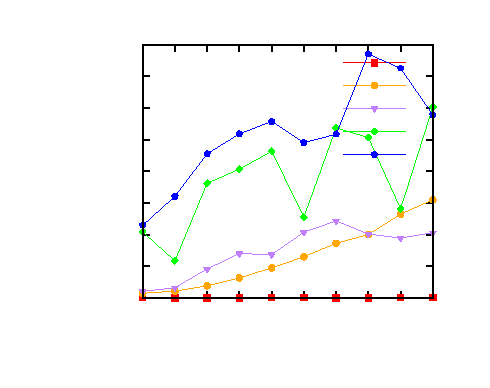
\includegraphics{bounds_epslatex/bounds_5_density_vs_time}}%
    \gplfronttext
  \end{picture}%
\endgroup

	% GNUPLOT: LaTeX picture with Postscript
\begingroup
  \makeatletter
  \providecommand\color[2][]{%
    \GenericError{(gnuplot) \space\space\space\@spaces}{%
      Package color not loaded in conjunction with
      terminal option `colourtext'%
    }{See the gnuplot documentation for explanation.%
    }{Either use 'blacktext' in gnuplot or load the package
      color.sty in LaTeX.}%
    \renewcommand\color[2][]{}%
  }%
  \providecommand\includegraphics[2][]{%
    \GenericError{(gnuplot) \space\space\space\@spaces}{%
      Package graphicx or graphics not loaded%
    }{See the gnuplot documentation for explanation.%
    }{The gnuplot epslatex terminal needs graphicx.sty or graphics.sty.}%
    \renewcommand\includegraphics[2][]{}%
  }%
  \providecommand\rotatebox[2]{#2}%
  \@ifundefined{ifGPcolor}{%
    \newif\ifGPcolor
    \GPcolorfalse
  }{}%
  \@ifundefined{ifGPblacktext}{%
    \newif\ifGPblacktext
    \GPblacktexttrue
  }{}%
  % define a \g@addto@macro without @ in the name:
  \let\gplgaddtomacro\g@addto@macro
  % define empty templates for all commands taking text:
  \gdef\gplbacktext{}%
  \gdef\gplfronttext{}%
  \makeatother
  \ifGPblacktext
    % no textcolor at all
    \def\colorrgb#1{}%
    \def\colorgray#1{}%
  \else
    % gray or color?
    \ifGPcolor
      \def\colorrgb#1{\color[rgb]{#1}}%
      \def\colorgray#1{\color[gray]{#1}}%
      \expandafter\def\csname LTw\endcsname{\color{white}}%
      \expandafter\def\csname LTb\endcsname{\color{black}}%
      \expandafter\def\csname LTa\endcsname{\color{black}}%
      \expandafter\def\csname LT0\endcsname{\color[rgb]{1,0,0}}%
      \expandafter\def\csname LT1\endcsname{\color[rgb]{0,1,0}}%
      \expandafter\def\csname LT2\endcsname{\color[rgb]{0,0,1}}%
      \expandafter\def\csname LT3\endcsname{\color[rgb]{1,0,1}}%
      \expandafter\def\csname LT4\endcsname{\color[rgb]{0,1,1}}%
      \expandafter\def\csname LT5\endcsname{\color[rgb]{1,1,0}}%
      \expandafter\def\csname LT6\endcsname{\color[rgb]{0,0,0}}%
      \expandafter\def\csname LT7\endcsname{\color[rgb]{1,0.3,0}}%
      \expandafter\def\csname LT8\endcsname{\color[rgb]{0.5,0.5,0.5}}%
    \else
      % gray
      \def\colorrgb#1{\color{black}}%
      \def\colorgray#1{\color[gray]{#1}}%
      \expandafter\def\csname LTw\endcsname{\color{white}}%
      \expandafter\def\csname LTb\endcsname{\color{black}}%
      \expandafter\def\csname LTa\endcsname{\color{black}}%
      \expandafter\def\csname LT0\endcsname{\color{black}}%
      \expandafter\def\csname LT1\endcsname{\color{black}}%
      \expandafter\def\csname LT2\endcsname{\color{black}}%
      \expandafter\def\csname LT3\endcsname{\color{black}}%
      \expandafter\def\csname LT4\endcsname{\color{black}}%
      \expandafter\def\csname LT5\endcsname{\color{black}}%
      \expandafter\def\csname LT6\endcsname{\color{black}}%
      \expandafter\def\csname LT7\endcsname{\color{black}}%
      \expandafter\def\csname LT8\endcsname{\color{black}}%
    \fi
  \fi
  \setlength{\unitlength}{0.0500bp}%
  \begin{picture}(4392.00,3400.00)%
    \gplgaddtomacro\gplbacktext{%
      \csname LTb\endcsname%
      \put(814,704){\makebox(0,0)[r]{\strut{} 0}}%
      \put(814,947){\makebox(0,0)[r]{\strut{} 2}}%
      \put(814,1190){\makebox(0,0)[r]{\strut{} 4}}%
      \put(814,1433){\makebox(0,0)[r]{\strut{} 6}}%
      \put(814,1676){\makebox(0,0)[r]{\strut{} 8}}%
      \put(814,1920){\makebox(0,0)[r]{\strut{} 10}}%
      \put(814,2163){\makebox(0,0)[r]{\strut{} 12}}%
      \put(814,2406){\makebox(0,0)[r]{\strut{} 14}}%
      \put(814,2649){\makebox(0,0)[r]{\strut{} 16}}%
      \put(814,2892){\makebox(0,0)[r]{\strut{} 18}}%
      \put(814,3135){\makebox(0,0)[r]{\strut{} 20}}%
      \put(946,484){\makebox(0,0){\strut{} 10}}%
      \put(1285,484){\makebox(0,0){\strut{} 20}}%
      \put(1624,484){\makebox(0,0){\strut{} 30}}%
      \put(1962,484){\makebox(0,0){\strut{} 40}}%
      \put(2301,484){\makebox(0,0){\strut{} 50}}%
      \put(2640,484){\makebox(0,0){\strut{} 60}}%
      \put(2979,484){\makebox(0,0){\strut{} 70}}%
      \put(3317,484){\makebox(0,0){\strut{} 80}}%
      \put(3656,484){\makebox(0,0){\strut{} 90}}%
      \put(3995,484){\makebox(0,0){\strut{} 100}}%
      \put(176,1919){\rotatebox{-270}{\makebox(0,0){\strut{}Tiempo de ejecuci\'on (ms)}}}%
      \put(2470,154){\makebox(0,0){\strut{}Porcentaje de clientes ($p$)}}%
    }%
    \gplgaddtomacro\gplfronttext{%
      \csname LTb\endcsname%
      \put(3008,2962){\makebox(0,0)[r]{\strut{}\texttt{dist\_x3}}}%
    }%
    \gplbacktext
    \put(0,0){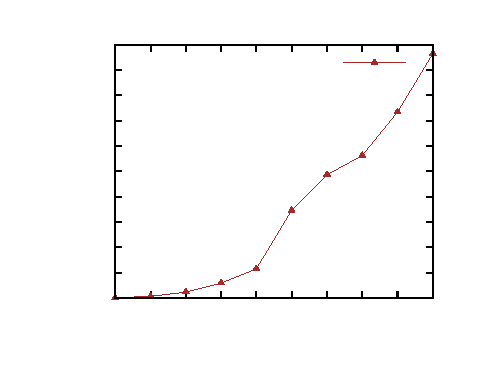
\includegraphics{bounds_epslatex/dist_x3_5_density_vs_time}}%
    \gplfronttext
  \end{picture}%
\endgroup

	\caption{Tiempos de ejecuci'on de las cotas para $n = 5$.}
	\label{fig:tiempos_5x5}
\end{figure}

\begin{figure}[h]
	% GNUPLOT: LaTeX picture with Postscript
\begingroup
  \makeatletter
  \providecommand\color[2][]{%
    \GenericError{(gnuplot) \space\space\space\@spaces}{%
      Package color not loaded in conjunction with
      terminal option `colourtext'%
    }{See the gnuplot documentation for explanation.%
    }{Either use 'blacktext' in gnuplot or load the package
      color.sty in LaTeX.}%
    \renewcommand\color[2][]{}%
  }%
  \providecommand\includegraphics[2][]{%
    \GenericError{(gnuplot) \space\space\space\@spaces}{%
      Package graphicx or graphics not loaded%
    }{See the gnuplot documentation for explanation.%
    }{The gnuplot epslatex terminal needs graphicx.sty or graphics.sty.}%
    \renewcommand\includegraphics[2][]{}%
  }%
  \providecommand\rotatebox[2]{#2}%
  \@ifundefined{ifGPcolor}{%
    \newif\ifGPcolor
    \GPcolorfalse
  }{}%
  \@ifundefined{ifGPblacktext}{%
    \newif\ifGPblacktext
    \GPblacktexttrue
  }{}%
  % define a \g@addto@macro without @ in the name:
  \let\gplgaddtomacro\g@addto@macro
  % define empty templates for all commands taking text:
  \gdef\gplbacktext{}%
  \gdef\gplfronttext{}%
  \makeatother
  \ifGPblacktext
    % no textcolor at all
    \def\colorrgb#1{}%
    \def\colorgray#1{}%
  \else
    % gray or color?
    \ifGPcolor
      \def\colorrgb#1{\color[rgb]{#1}}%
      \def\colorgray#1{\color[gray]{#1}}%
      \expandafter\def\csname LTw\endcsname{\color{white}}%
      \expandafter\def\csname LTb\endcsname{\color{black}}%
      \expandafter\def\csname LTa\endcsname{\color{black}}%
      \expandafter\def\csname LT0\endcsname{\color[rgb]{1,0,0}}%
      \expandafter\def\csname LT1\endcsname{\color[rgb]{0,1,0}}%
      \expandafter\def\csname LT2\endcsname{\color[rgb]{0,0,1}}%
      \expandafter\def\csname LT3\endcsname{\color[rgb]{1,0,1}}%
      \expandafter\def\csname LT4\endcsname{\color[rgb]{0,1,1}}%
      \expandafter\def\csname LT5\endcsname{\color[rgb]{1,1,0}}%
      \expandafter\def\csname LT6\endcsname{\color[rgb]{0,0,0}}%
      \expandafter\def\csname LT7\endcsname{\color[rgb]{1,0.3,0}}%
      \expandafter\def\csname LT8\endcsname{\color[rgb]{0.5,0.5,0.5}}%
    \else
      % gray
      \def\colorrgb#1{\color{black}}%
      \def\colorgray#1{\color[gray]{#1}}%
      \expandafter\def\csname LTw\endcsname{\color{white}}%
      \expandafter\def\csname LTb\endcsname{\color{black}}%
      \expandafter\def\csname LTa\endcsname{\color{black}}%
      \expandafter\def\csname LT0\endcsname{\color{black}}%
      \expandafter\def\csname LT1\endcsname{\color{black}}%
      \expandafter\def\csname LT2\endcsname{\color{black}}%
      \expandafter\def\csname LT3\endcsname{\color{black}}%
      \expandafter\def\csname LT4\endcsname{\color{black}}%
      \expandafter\def\csname LT5\endcsname{\color{black}}%
      \expandafter\def\csname LT6\endcsname{\color{black}}%
      \expandafter\def\csname LT7\endcsname{\color{black}}%
      \expandafter\def\csname LT8\endcsname{\color{black}}%
    \fi
  \fi
  \setlength{\unitlength}{0.0500bp}%
  \begin{picture}(4392.00,3400.00)%
    \gplgaddtomacro\gplbacktext{%
      \csname LTb\endcsname%
      \put(946,704){\makebox(0,0)[r]{\strut{} 0}}%
      \put(946,1051){\makebox(0,0)[r]{\strut{} 0.2}}%
      \put(946,1399){\makebox(0,0)[r]{\strut{} 0.4}}%
      \put(946,1746){\makebox(0,0)[r]{\strut{} 0.6}}%
      \put(946,2093){\makebox(0,0)[r]{\strut{} 0.8}}%
      \put(946,2440){\makebox(0,0)[r]{\strut{} 1}}%
      \put(946,2788){\makebox(0,0)[r]{\strut{} 1.2}}%
      \put(946,3135){\makebox(0,0)[r]{\strut{} 1.4}}%
      \put(1078,484){\makebox(0,0){\strut{} 10}}%
      \put(1402,484){\makebox(0,0){\strut{} 20}}%
      \put(1726,484){\makebox(0,0){\strut{} 30}}%
      \put(2050,484){\makebox(0,0){\strut{} 40}}%
      \put(2374,484){\makebox(0,0){\strut{} 50}}%
      \put(2699,484){\makebox(0,0){\strut{} 60}}%
      \put(3023,484){\makebox(0,0){\strut{} 70}}%
      \put(3347,484){\makebox(0,0){\strut{} 80}}%
      \put(3671,484){\makebox(0,0){\strut{} 90}}%
      \put(3995,484){\makebox(0,0){\strut{} 100}}%
      \put(176,1919){\rotatebox{-270}{\makebox(0,0){\strut{}Tiempo de ejecuci\'on (ms)}}}%
      \put(2536,154){\makebox(0,0){\strut{}Porcentaje de clientes ($p$)}}%
    }%
    \gplgaddtomacro\gplfronttext{%
      \csname LTb\endcsname%
      \put(3008,2962){\makebox(0,0)[r]{\strut{}\texttt{clients\_count}}}%
      \csname LTb\endcsname%
      \put(3008,2742){\makebox(0,0)[r]{\strut{}\texttt{dist\_x2}}}%
      \csname LTb\endcsname%
      \put(3008,2522){\makebox(0,0)[r]{\strut{}\texttt{mst}}}%
      \csname LTb\endcsname%
      \put(3008,2302){\makebox(0,0)[r]{\strut{}\texttt{vc}}}%
      \csname LTb\endcsname%
      \put(3008,2082){\makebox(0,0)[r]{\strut{}\texttt{vc\_mst}}}%
    }%
    \gplbacktext
    \put(0,0){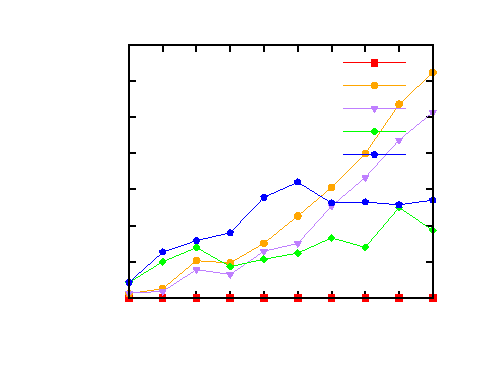
\includegraphics{bounds_epslatex/bounds_10_density_vs_time}}%
    \gplfronttext
  \end{picture}%
\endgroup

	% GNUPLOT: LaTeX picture with Postscript
\begingroup
  \makeatletter
  \providecommand\color[2][]{%
    \GenericError{(gnuplot) \space\space\space\@spaces}{%
      Package color not loaded in conjunction with
      terminal option `colourtext'%
    }{See the gnuplot documentation for explanation.%
    }{Either use 'blacktext' in gnuplot or load the package
      color.sty in LaTeX.}%
    \renewcommand\color[2][]{}%
  }%
  \providecommand\includegraphics[2][]{%
    \GenericError{(gnuplot) \space\space\space\@spaces}{%
      Package graphicx or graphics not loaded%
    }{See the gnuplot documentation for explanation.%
    }{The gnuplot epslatex terminal needs graphicx.sty or graphics.sty.}%
    \renewcommand\includegraphics[2][]{}%
  }%
  \providecommand\rotatebox[2]{#2}%
  \@ifundefined{ifGPcolor}{%
    \newif\ifGPcolor
    \GPcolorfalse
  }{}%
  \@ifundefined{ifGPblacktext}{%
    \newif\ifGPblacktext
    \GPblacktexttrue
  }{}%
  % define a \g@addto@macro without @ in the name:
  \let\gplgaddtomacro\g@addto@macro
  % define empty templates for all commands taking text:
  \gdef\gplbacktext{}%
  \gdef\gplfronttext{}%
  \makeatother
  \ifGPblacktext
    % no textcolor at all
    \def\colorrgb#1{}%
    \def\colorgray#1{}%
  \else
    % gray or color?
    \ifGPcolor
      \def\colorrgb#1{\color[rgb]{#1}}%
      \def\colorgray#1{\color[gray]{#1}}%
      \expandafter\def\csname LTw\endcsname{\color{white}}%
      \expandafter\def\csname LTb\endcsname{\color{black}}%
      \expandafter\def\csname LTa\endcsname{\color{black}}%
      \expandafter\def\csname LT0\endcsname{\color[rgb]{1,0,0}}%
      \expandafter\def\csname LT1\endcsname{\color[rgb]{0,1,0}}%
      \expandafter\def\csname LT2\endcsname{\color[rgb]{0,0,1}}%
      \expandafter\def\csname LT3\endcsname{\color[rgb]{1,0,1}}%
      \expandafter\def\csname LT4\endcsname{\color[rgb]{0,1,1}}%
      \expandafter\def\csname LT5\endcsname{\color[rgb]{1,1,0}}%
      \expandafter\def\csname LT6\endcsname{\color[rgb]{0,0,0}}%
      \expandafter\def\csname LT7\endcsname{\color[rgb]{1,0.3,0}}%
      \expandafter\def\csname LT8\endcsname{\color[rgb]{0.5,0.5,0.5}}%
    \else
      % gray
      \def\colorrgb#1{\color{black}}%
      \def\colorgray#1{\color[gray]{#1}}%
      \expandafter\def\csname LTw\endcsname{\color{white}}%
      \expandafter\def\csname LTb\endcsname{\color{black}}%
      \expandafter\def\csname LTa\endcsname{\color{black}}%
      \expandafter\def\csname LT0\endcsname{\color{black}}%
      \expandafter\def\csname LT1\endcsname{\color{black}}%
      \expandafter\def\csname LT2\endcsname{\color{black}}%
      \expandafter\def\csname LT3\endcsname{\color{black}}%
      \expandafter\def\csname LT4\endcsname{\color{black}}%
      \expandafter\def\csname LT5\endcsname{\color{black}}%
      \expandafter\def\csname LT6\endcsname{\color{black}}%
      \expandafter\def\csname LT7\endcsname{\color{black}}%
      \expandafter\def\csname LT8\endcsname{\color{black}}%
    \fi
  \fi
  \setlength{\unitlength}{0.0500bp}%
  \begin{picture}(4392.00,3400.00)%
    \gplgaddtomacro\gplbacktext{%
      \csname LTb\endcsname%
      \put(1078,704){\makebox(0,0)[r]{\strut{} 0}}%
      \put(1078,1051){\makebox(0,0)[r]{\strut{} 200}}%
      \put(1078,1399){\makebox(0,0)[r]{\strut{} 400}}%
      \put(1078,1746){\makebox(0,0)[r]{\strut{} 600}}%
      \put(1078,2093){\makebox(0,0)[r]{\strut{} 800}}%
      \put(1078,2440){\makebox(0,0)[r]{\strut{} 1000}}%
      \put(1078,2788){\makebox(0,0)[r]{\strut{} 1200}}%
      \put(1078,3135){\makebox(0,0)[r]{\strut{} 1400}}%
      \put(1210,484){\makebox(0,0){\strut{} 10}}%
      \put(1519,484){\makebox(0,0){\strut{} 20}}%
      \put(1829,484){\makebox(0,0){\strut{} 30}}%
      \put(2138,484){\makebox(0,0){\strut{} 40}}%
      \put(2448,484){\makebox(0,0){\strut{} 50}}%
      \put(2757,484){\makebox(0,0){\strut{} 60}}%
      \put(3067,484){\makebox(0,0){\strut{} 70}}%
      \put(3376,484){\makebox(0,0){\strut{} 80}}%
      \put(3686,484){\makebox(0,0){\strut{} 90}}%
      \put(3995,484){\makebox(0,0){\strut{} 100}}%
      \put(176,1919){\rotatebox{-270}{\makebox(0,0){\strut{}Tiempo de ejecuci\'on (ms)}}}%
      \put(2602,154){\makebox(0,0){\strut{}Porcentaje de clientes ($p$)}}%
    }%
    \gplgaddtomacro\gplfronttext{%
      \csname LTb\endcsname%
      \put(3008,2962){\makebox(0,0)[r]{\strut{}\texttt{dist\_x3}}}%
    }%
    \gplbacktext
    \put(0,0){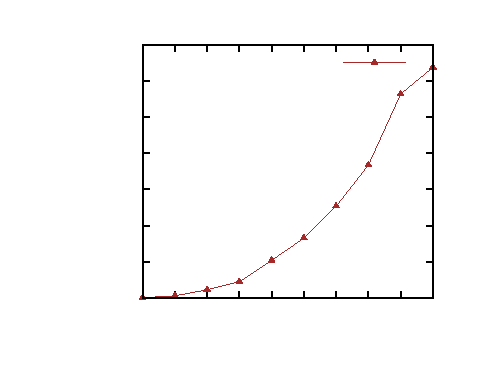
\includegraphics{bounds_epslatex/dist_x3_10_density_vs_time}}%
    \gplfronttext
  \end{picture}%
\endgroup

	\caption{Tiempos de ejecuci'on de las cotas para $n = 10$.}
	\label{fig:tiempos_10x10}
\end{figure}

\begin{figure}[h]
	% GNUPLOT: LaTeX picture with Postscript
\begingroup
  \makeatletter
  \providecommand\color[2][]{%
    \GenericError{(gnuplot) \space\space\space\@spaces}{%
      Package color not loaded in conjunction with
      terminal option `colourtext'%
    }{See the gnuplot documentation for explanation.%
    }{Either use 'blacktext' in gnuplot or load the package
      color.sty in LaTeX.}%
    \renewcommand\color[2][]{}%
  }%
  \providecommand\includegraphics[2][]{%
    \GenericError{(gnuplot) \space\space\space\@spaces}{%
      Package graphicx or graphics not loaded%
    }{See the gnuplot documentation for explanation.%
    }{The gnuplot epslatex terminal needs graphicx.sty or graphics.sty.}%
    \renewcommand\includegraphics[2][]{}%
  }%
  \providecommand\rotatebox[2]{#2}%
  \@ifundefined{ifGPcolor}{%
    \newif\ifGPcolor
    \GPcolorfalse
  }{}%
  \@ifundefined{ifGPblacktext}{%
    \newif\ifGPblacktext
    \GPblacktexttrue
  }{}%
  % define a \g@addto@macro without @ in the name:
  \let\gplgaddtomacro\g@addto@macro
  % define empty templates for all commands taking text:
  \gdef\gplbacktext{}%
  \gdef\gplfronttext{}%
  \makeatother
  \ifGPblacktext
    % no textcolor at all
    \def\colorrgb#1{}%
    \def\colorgray#1{}%
  \else
    % gray or color?
    \ifGPcolor
      \def\colorrgb#1{\color[rgb]{#1}}%
      \def\colorgray#1{\color[gray]{#1}}%
      \expandafter\def\csname LTw\endcsname{\color{white}}%
      \expandafter\def\csname LTb\endcsname{\color{black}}%
      \expandafter\def\csname LTa\endcsname{\color{black}}%
      \expandafter\def\csname LT0\endcsname{\color[rgb]{1,0,0}}%
      \expandafter\def\csname LT1\endcsname{\color[rgb]{0,1,0}}%
      \expandafter\def\csname LT2\endcsname{\color[rgb]{0,0,1}}%
      \expandafter\def\csname LT3\endcsname{\color[rgb]{1,0,1}}%
      \expandafter\def\csname LT4\endcsname{\color[rgb]{0,1,1}}%
      \expandafter\def\csname LT5\endcsname{\color[rgb]{1,1,0}}%
      \expandafter\def\csname LT6\endcsname{\color[rgb]{0,0,0}}%
      \expandafter\def\csname LT7\endcsname{\color[rgb]{1,0.3,0}}%
      \expandafter\def\csname LT8\endcsname{\color[rgb]{0.5,0.5,0.5}}%
    \else
      % gray
      \def\colorrgb#1{\color{black}}%
      \def\colorgray#1{\color[gray]{#1}}%
      \expandafter\def\csname LTw\endcsname{\color{white}}%
      \expandafter\def\csname LTb\endcsname{\color{black}}%
      \expandafter\def\csname LTa\endcsname{\color{black}}%
      \expandafter\def\csname LT0\endcsname{\color{black}}%
      \expandafter\def\csname LT1\endcsname{\color{black}}%
      \expandafter\def\csname LT2\endcsname{\color{black}}%
      \expandafter\def\csname LT3\endcsname{\color{black}}%
      \expandafter\def\csname LT4\endcsname{\color{black}}%
      \expandafter\def\csname LT5\endcsname{\color{black}}%
      \expandafter\def\csname LT6\endcsname{\color{black}}%
      \expandafter\def\csname LT7\endcsname{\color{black}}%
      \expandafter\def\csname LT8\endcsname{\color{black}}%
    \fi
  \fi
  \setlength{\unitlength}{0.0500bp}%
  \begin{picture}(4392.00,3400.00)%
    \gplgaddtomacro\gplbacktext{%
      \csname LTb\endcsname%
      \put(946,704){\makebox(0,0)[r]{\strut{} 0}}%
      \put(946,1051){\makebox(0,0)[r]{\strut{} 20}}%
      \put(946,1399){\makebox(0,0)[r]{\strut{} 40}}%
      \put(946,1746){\makebox(0,0)[r]{\strut{} 60}}%
      \put(946,2093){\makebox(0,0)[r]{\strut{} 80}}%
      \put(946,2440){\makebox(0,0)[r]{\strut{} 100}}%
      \put(946,2788){\makebox(0,0)[r]{\strut{} 120}}%
      \put(946,3135){\makebox(0,0)[r]{\strut{} 140}}%
      \put(1078,484){\makebox(0,0){\strut{} 10}}%
      \put(1402,484){\makebox(0,0){\strut{} 20}}%
      \put(1726,484){\makebox(0,0){\strut{} 30}}%
      \put(2050,484){\makebox(0,0){\strut{} 40}}%
      \put(2374,484){\makebox(0,0){\strut{} 50}}%
      \put(2699,484){\makebox(0,0){\strut{} 60}}%
      \put(3023,484){\makebox(0,0){\strut{} 70}}%
      \put(3347,484){\makebox(0,0){\strut{} 80}}%
      \put(3671,484){\makebox(0,0){\strut{} 90}}%
      \put(3995,484){\makebox(0,0){\strut{} 100}}%
      \put(176,1919){\rotatebox{-270}{\makebox(0,0){\strut{}Tiempo de ejecuci\'on (ms)}}}%
      \put(2536,154){\makebox(0,0){\strut{}Porcentaje de clientes ($p$)}}%
    }%
    \gplgaddtomacro\gplfronttext{%
      \csname LTb\endcsname%
      \put(3008,2962){\makebox(0,0)[r]{\strut{}\texttt{clients\_count}}}%
      \csname LTb\endcsname%
      \put(3008,2742){\makebox(0,0)[r]{\strut{}\texttt{dist\_x2}}}%
      \csname LTb\endcsname%
      \put(3008,2522){\makebox(0,0)[r]{\strut{}\texttt{mst}}}%
      \csname LTb\endcsname%
      \put(3008,2302){\makebox(0,0)[r]{\strut{}\texttt{vc}}}%
      \csname LTb\endcsname%
      \put(3008,2082){\makebox(0,0)[r]{\strut{}\texttt{vc\_mst}}}%
    }%
    \gplbacktext
    \put(0,0){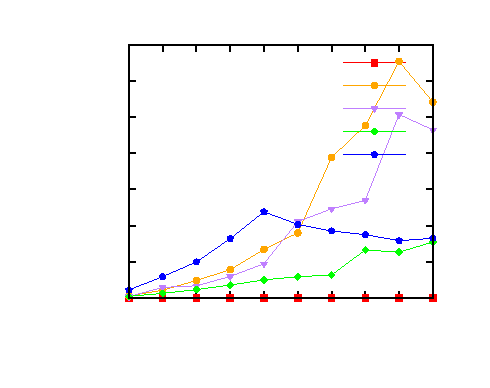
\includegraphics{bounds_epslatex/bounds_30_density_vs_time}}%
    \gplfronttext
  \end{picture}%
\endgroup

	% GNUPLOT: LaTeX picture with Postscript
\begingroup
  \makeatletter
  \providecommand\color[2][]{%
    \GenericError{(gnuplot) \space\space\space\@spaces}{%
      Package color not loaded in conjunction with
      terminal option `colourtext'%
    }{See the gnuplot documentation for explanation.%
    }{Either use 'blacktext' in gnuplot or load the package
      color.sty in LaTeX.}%
    \renewcommand\color[2][]{}%
  }%
  \providecommand\includegraphics[2][]{%
    \GenericError{(gnuplot) \space\space\space\@spaces}{%
      Package graphicx or graphics not loaded%
    }{See the gnuplot documentation for explanation.%
    }{The gnuplot epslatex terminal needs graphicx.sty or graphics.sty.}%
    \renewcommand\includegraphics[2][]{}%
  }%
  \providecommand\rotatebox[2]{#2}%
  \@ifundefined{ifGPcolor}{%
    \newif\ifGPcolor
    \GPcolorfalse
  }{}%
  \@ifundefined{ifGPblacktext}{%
    \newif\ifGPblacktext
    \GPblacktexttrue
  }{}%
  % define a \g@addto@macro without @ in the name:
  \let\gplgaddtomacro\g@addto@macro
  % define empty templates for all commands taking text:
  \gdef\gplbacktext{}%
  \gdef\gplfronttext{}%
  \makeatother
  \ifGPblacktext
    % no textcolor at all
    \def\colorrgb#1{}%
    \def\colorgray#1{}%
  \else
    % gray or color?
    \ifGPcolor
      \def\colorrgb#1{\color[rgb]{#1}}%
      \def\colorgray#1{\color[gray]{#1}}%
      \expandafter\def\csname LTw\endcsname{\color{white}}%
      \expandafter\def\csname LTb\endcsname{\color{black}}%
      \expandafter\def\csname LTa\endcsname{\color{black}}%
      \expandafter\def\csname LT0\endcsname{\color[rgb]{1,0,0}}%
      \expandafter\def\csname LT1\endcsname{\color[rgb]{0,1,0}}%
      \expandafter\def\csname LT2\endcsname{\color[rgb]{0,0,1}}%
      \expandafter\def\csname LT3\endcsname{\color[rgb]{1,0,1}}%
      \expandafter\def\csname LT4\endcsname{\color[rgb]{0,1,1}}%
      \expandafter\def\csname LT5\endcsname{\color[rgb]{1,1,0}}%
      \expandafter\def\csname LT6\endcsname{\color[rgb]{0,0,0}}%
      \expandafter\def\csname LT7\endcsname{\color[rgb]{1,0.3,0}}%
      \expandafter\def\csname LT8\endcsname{\color[rgb]{0.5,0.5,0.5}}%
    \else
      % gray
      \def\colorrgb#1{\color{black}}%
      \def\colorgray#1{\color[gray]{#1}}%
      \expandafter\def\csname LTw\endcsname{\color{white}}%
      \expandafter\def\csname LTb\endcsname{\color{black}}%
      \expandafter\def\csname LTa\endcsname{\color{black}}%
      \expandafter\def\csname LT0\endcsname{\color{black}}%
      \expandafter\def\csname LT1\endcsname{\color{black}}%
      \expandafter\def\csname LT2\endcsname{\color{black}}%
      \expandafter\def\csname LT3\endcsname{\color{black}}%
      \expandafter\def\csname LT4\endcsname{\color{black}}%
      \expandafter\def\csname LT5\endcsname{\color{black}}%
      \expandafter\def\csname LT6\endcsname{\color{black}}%
      \expandafter\def\csname LT7\endcsname{\color{black}}%
      \expandafter\def\csname LT8\endcsname{\color{black}}%
    \fi
  \fi
  \setlength{\unitlength}{0.0500bp}%
  \begin{picture}(4392.00,3400.00)%
    \gplgaddtomacro\gplbacktext{%
      \csname LTb\endcsname%
      \put(1474,704){\makebox(0,0)[r]{\strut{} 0}}%
      \put(1474,1051){\makebox(0,0)[r]{\strut{} 200000}}%
      \put(1474,1399){\makebox(0,0)[r]{\strut{} 400000}}%
      \put(1474,1746){\makebox(0,0)[r]{\strut{} 600000}}%
      \put(1474,2093){\makebox(0,0)[r]{\strut{} 800000}}%
      \put(1474,2440){\makebox(0,0)[r]{\strut{} 1e+06}}%
      \put(1474,2788){\makebox(0,0)[r]{\strut{} 1.2e+06}}%
      \put(1474,3135){\makebox(0,0)[r]{\strut{} 1.4e+06}}%
      \put(1606,484){\makebox(0,0){\strut{} 10}}%
      \put(1871,484){\makebox(0,0){\strut{} 20}}%
      \put(2137,484){\makebox(0,0){\strut{} 30}}%
      \put(2402,484){\makebox(0,0){\strut{} 40}}%
      \put(2668,484){\makebox(0,0){\strut{} 50}}%
      \put(2933,484){\makebox(0,0){\strut{} 60}}%
      \put(3199,484){\makebox(0,0){\strut{} 70}}%
      \put(3464,484){\makebox(0,0){\strut{} 80}}%
      \put(3730,484){\makebox(0,0){\strut{} 90}}%
      \put(3995,484){\makebox(0,0){\strut{} 100}}%
      \put(176,1919){\rotatebox{-270}{\makebox(0,0){\strut{}Tiempo de ejecuci\'on (ms)}}}%
      \put(2800,154){\makebox(0,0){\strut{}Porcentaje de clientes ($p$)}}%
    }%
    \gplgaddtomacro\gplfronttext{%
      \csname LTb\endcsname%
      \put(3008,2962){\makebox(0,0)[r]{\strut{}\texttt{dist\_x3}}}%
    }%
    \gplbacktext
    \put(0,0){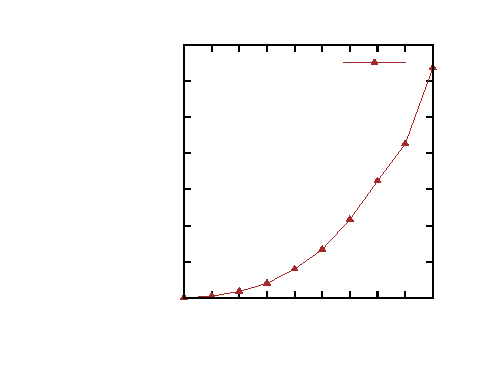
\includegraphics{bounds_epslatex/dist_x3_30_density_vs_time}}%
    \gplfronttext
  \end{picture}%
\endgroup

	\caption{Tiempos de ejecuci'on de las cotas para $n = 30$.}
	\label{fig:tiempos_30x30}
\end{figure}

\begin{figure}[h]
	\centering
	% GNUPLOT: LaTeX picture with Postscript
\begingroup
  \makeatletter
  \providecommand\color[2][]{%
    \GenericError{(gnuplot) \space\space\space\@spaces}{%
      Package color not loaded in conjunction with
      terminal option `colourtext'%
    }{See the gnuplot documentation for explanation.%
    }{Either use 'blacktext' in gnuplot or load the package
      color.sty in LaTeX.}%
    \renewcommand\color[2][]{}%
  }%
  \providecommand\includegraphics[2][]{%
    \GenericError{(gnuplot) \space\space\space\@spaces}{%
      Package graphicx or graphics not loaded%
    }{See the gnuplot documentation for explanation.%
    }{The gnuplot epslatex terminal needs graphicx.sty or graphics.sty.}%
    \renewcommand\includegraphics[2][]{}%
  }%
  \providecommand\rotatebox[2]{#2}%
  \@ifundefined{ifGPcolor}{%
    \newif\ifGPcolor
    \GPcolorfalse
  }{}%
  \@ifundefined{ifGPblacktext}{%
    \newif\ifGPblacktext
    \GPblacktexttrue
  }{}%
  % define a \g@addto@macro without @ in the name:
  \let\gplgaddtomacro\g@addto@macro
  % define empty templates for all commands taking text:
  \gdef\gplbacktext{}%
  \gdef\gplfronttext{}%
  \makeatother
  \ifGPblacktext
    % no textcolor at all
    \def\colorrgb#1{}%
    \def\colorgray#1{}%
  \else
    % gray or color?
    \ifGPcolor
      \def\colorrgb#1{\color[rgb]{#1}}%
      \def\colorgray#1{\color[gray]{#1}}%
      \expandafter\def\csname LTw\endcsname{\color{white}}%
      \expandafter\def\csname LTb\endcsname{\color{black}}%
      \expandafter\def\csname LTa\endcsname{\color{black}}%
      \expandafter\def\csname LT0\endcsname{\color[rgb]{1,0,0}}%
      \expandafter\def\csname LT1\endcsname{\color[rgb]{0,1,0}}%
      \expandafter\def\csname LT2\endcsname{\color[rgb]{0,0,1}}%
      \expandafter\def\csname LT3\endcsname{\color[rgb]{1,0,1}}%
      \expandafter\def\csname LT4\endcsname{\color[rgb]{0,1,1}}%
      \expandafter\def\csname LT5\endcsname{\color[rgb]{1,1,0}}%
      \expandafter\def\csname LT6\endcsname{\color[rgb]{0,0,0}}%
      \expandafter\def\csname LT7\endcsname{\color[rgb]{1,0.3,0}}%
      \expandafter\def\csname LT8\endcsname{\color[rgb]{0.5,0.5,0.5}}%
    \else
      % gray
      \def\colorrgb#1{\color{black}}%
      \def\colorgray#1{\color[gray]{#1}}%
      \expandafter\def\csname LTw\endcsname{\color{white}}%
      \expandafter\def\csname LTb\endcsname{\color{black}}%
      \expandafter\def\csname LTa\endcsname{\color{black}}%
      \expandafter\def\csname LT0\endcsname{\color{black}}%
      \expandafter\def\csname LT1\endcsname{\color{black}}%
      \expandafter\def\csname LT2\endcsname{\color{black}}%
      \expandafter\def\csname LT3\endcsname{\color{black}}%
      \expandafter\def\csname LT4\endcsname{\color{black}}%
      \expandafter\def\csname LT5\endcsname{\color{black}}%
      \expandafter\def\csname LT6\endcsname{\color{black}}%
      \expandafter\def\csname LT7\endcsname{\color{black}}%
      \expandafter\def\csname LT8\endcsname{\color{black}}%
    \fi
  \fi
  \setlength{\unitlength}{0.0500bp}%
  \begin{picture}(4392.00,3400.00)%
    \gplgaddtomacro\gplbacktext{%
      \csname LTb\endcsname%
      \put(946,704){\makebox(0,0)[r]{\strut{} 0}}%
      \put(946,974){\makebox(0,0)[r]{\strut{} 100}}%
      \put(946,1244){\makebox(0,0)[r]{\strut{} 200}}%
      \put(946,1514){\makebox(0,0)[r]{\strut{} 300}}%
      \put(946,1784){\makebox(0,0)[r]{\strut{} 400}}%
      \put(946,2055){\makebox(0,0)[r]{\strut{} 500}}%
      \put(946,2325){\makebox(0,0)[r]{\strut{} 600}}%
      \put(946,2595){\makebox(0,0)[r]{\strut{} 700}}%
      \put(946,2865){\makebox(0,0)[r]{\strut{} 800}}%
      \put(946,3135){\makebox(0,0)[r]{\strut{} 900}}%
      \put(1078,484){\makebox(0,0){\strut{} 10}}%
      \put(1402,484){\makebox(0,0){\strut{} 20}}%
      \put(1726,484){\makebox(0,0){\strut{} 30}}%
      \put(2050,484){\makebox(0,0){\strut{} 40}}%
      \put(2374,484){\makebox(0,0){\strut{} 50}}%
      \put(2699,484){\makebox(0,0){\strut{} 60}}%
      \put(3023,484){\makebox(0,0){\strut{} 70}}%
      \put(3347,484){\makebox(0,0){\strut{} 80}}%
      \put(3671,484){\makebox(0,0){\strut{} 90}}%
      \put(3995,484){\makebox(0,0){\strut{} 100}}%
      \put(176,1919){\rotatebox{-270}{\makebox(0,0){\strut{}Tiempo de ejecuci\'on (ms)}}}%
      \put(2536,154){\makebox(0,0){\strut{}Porcentaje de clientes ($p$)}}%
    }%
    \gplgaddtomacro\gplfronttext{%
      \csname LTb\endcsname%
      \put(3008,2962){\makebox(0,0)[r]{\strut{}\texttt{clients\_count}}}%
      \csname LTb\endcsname%
      \put(3008,2742){\makebox(0,0)[r]{\strut{}\texttt{dist\_x2}}}%
      \csname LTb\endcsname%
      \put(3008,2522){\makebox(0,0)[r]{\strut{}\texttt{mst}}}%
      \csname LTb\endcsname%
      \put(3008,2302){\makebox(0,0)[r]{\strut{}\texttt{vc}}}%
      \csname LTb\endcsname%
      \put(3008,2082){\makebox(0,0)[r]{\strut{}\texttt{vc\_mst}}}%
    }%
    \gplbacktext
    \put(0,0){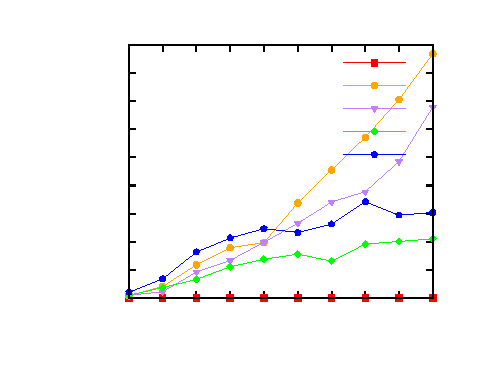
\includegraphics{bounds_epslatex/bounds_50_density_vs_time}}%
    \gplfronttext
  \end{picture}%
\endgroup

	\caption{Tiempos de ejecuci'on de las cotas para $n = 50$.}
	\label{fig:tiempos_50x50}
\end{figure}

\begin{figure}[h]
\begin{minipage}[t]{0.45\textwidth}
	\centering
	% GNUPLOT: LaTeX picture with Postscript
\begingroup
  \makeatletter
  \providecommand\color[2][]{%
    \GenericError{(gnuplot) \space\space\space\@spaces}{%
      Package color not loaded in conjunction with
      terminal option `colourtext'%
    }{See the gnuplot documentation for explanation.%
    }{Either use 'blacktext' in gnuplot or load the package
      color.sty in LaTeX.}%
    \renewcommand\color[2][]{}%
  }%
  \providecommand\includegraphics[2][]{%
    \GenericError{(gnuplot) \space\space\space\@spaces}{%
      Package graphicx or graphics not loaded%
    }{See the gnuplot documentation for explanation.%
    }{The gnuplot epslatex terminal needs graphicx.sty or graphics.sty.}%
    \renewcommand\includegraphics[2][]{}%
  }%
  \providecommand\rotatebox[2]{#2}%
  \@ifundefined{ifGPcolor}{%
    \newif\ifGPcolor
    \GPcolorfalse
  }{}%
  \@ifundefined{ifGPblacktext}{%
    \newif\ifGPblacktext
    \GPblacktexttrue
  }{}%
  % define a \g@addto@macro without @ in the name:
  \let\gplgaddtomacro\g@addto@macro
  % define empty templates for all commands taking text:
  \gdef\gplbacktext{}%
  \gdef\gplfronttext{}%
  \makeatother
  \ifGPblacktext
    % no textcolor at all
    \def\colorrgb#1{}%
    \def\colorgray#1{}%
  \else
    % gray or color?
    \ifGPcolor
      \def\colorrgb#1{\color[rgb]{#1}}%
      \def\colorgray#1{\color[gray]{#1}}%
      \expandafter\def\csname LTw\endcsname{\color{white}}%
      \expandafter\def\csname LTb\endcsname{\color{black}}%
      \expandafter\def\csname LTa\endcsname{\color{black}}%
      \expandafter\def\csname LT0\endcsname{\color[rgb]{1,0,0}}%
      \expandafter\def\csname LT1\endcsname{\color[rgb]{0,1,0}}%
      \expandafter\def\csname LT2\endcsname{\color[rgb]{0,0,1}}%
      \expandafter\def\csname LT3\endcsname{\color[rgb]{1,0,1}}%
      \expandafter\def\csname LT4\endcsname{\color[rgb]{0,1,1}}%
      \expandafter\def\csname LT5\endcsname{\color[rgb]{1,1,0}}%
      \expandafter\def\csname LT6\endcsname{\color[rgb]{0,0,0}}%
      \expandafter\def\csname LT7\endcsname{\color[rgb]{1,0.3,0}}%
      \expandafter\def\csname LT8\endcsname{\color[rgb]{0.5,0.5,0.5}}%
    \else
      % gray
      \def\colorrgb#1{\color{black}}%
      \def\colorgray#1{\color[gray]{#1}}%
      \expandafter\def\csname LTw\endcsname{\color{white}}%
      \expandafter\def\csname LTb\endcsname{\color{black}}%
      \expandafter\def\csname LTa\endcsname{\color{black}}%
      \expandafter\def\csname LT0\endcsname{\color{black}}%
      \expandafter\def\csname LT1\endcsname{\color{black}}%
      \expandafter\def\csname LT2\endcsname{\color{black}}%
      \expandafter\def\csname LT3\endcsname{\color{black}}%
      \expandafter\def\csname LT4\endcsname{\color{black}}%
      \expandafter\def\csname LT5\endcsname{\color{black}}%
      \expandafter\def\csname LT6\endcsname{\color{black}}%
      \expandafter\def\csname LT7\endcsname{\color{black}}%
      \expandafter\def\csname LT8\endcsname{\color{black}}%
    \fi
  \fi
  \setlength{\unitlength}{0.0500bp}%
  \begin{picture}(4392.00,3400.00)%
    \gplgaddtomacro\gplbacktext{%
      \csname LTb\endcsname%
      \put(814,704){\makebox(0,0)[r]{\strut{} 0}}%
      \put(814,1109){\makebox(0,0)[r]{\strut{} 2}}%
      \put(814,1514){\makebox(0,0)[r]{\strut{} 4}}%
      \put(814,1920){\makebox(0,0)[r]{\strut{} 6}}%
      \put(814,2325){\makebox(0,0)[r]{\strut{} 8}}%
      \put(814,2730){\makebox(0,0)[r]{\strut{} 10}}%
      \put(814,3135){\makebox(0,0)[r]{\strut{} 12}}%
      \put(946,484){\makebox(0,0){\strut{} 10}}%
      \put(1285,484){\makebox(0,0){\strut{} 20}}%
      \put(1624,484){\makebox(0,0){\strut{} 30}}%
      \put(1962,484){\makebox(0,0){\strut{} 40}}%
      \put(2301,484){\makebox(0,0){\strut{} 50}}%
      \put(2640,484){\makebox(0,0){\strut{} 60}}%
      \put(2979,484){\makebox(0,0){\strut{} 70}}%
      \put(3317,484){\makebox(0,0){\strut{} 80}}%
      \put(3656,484){\makebox(0,0){\strut{} 90}}%
      \put(3995,484){\makebox(0,0){\strut{} 100}}%
      \put(176,1919){\rotatebox{-270}{\makebox(0,0){\strut{}Valor de la funci\'on}}}%
      \put(2470,154){\makebox(0,0){\strut{}Porcentaje de clientes ($p$)}}%
    }%
    \gplgaddtomacro\gplfronttext{%
      \csname LTb\endcsname%
      \put(3008,2962){\makebox(0,0)[r]{\strut{}\texttt{clients\_count}}}%
      \csname LTb\endcsname%
      \put(3008,2742){\makebox(0,0)[r]{\strut{}\texttt{dist\_x2}}}%
      \csname LTb\endcsname%
      \put(3008,2522){\makebox(0,0)[r]{\strut{}\texttt{dist\_x3}}}%
      \csname LTb\endcsname%
      \put(3008,2302){\makebox(0,0)[r]{\strut{}\texttt{mst}}}%
      \csname LTb\endcsname%
      \put(3008,2082){\makebox(0,0)[r]{\strut{}\texttt{vc}}}%
      \csname LTb\endcsname%
      \put(3008,1862){\makebox(0,0)[r]{\strut{}\texttt{vc\_mst}}}%
    }%
    \gplbacktext
    \put(0,0){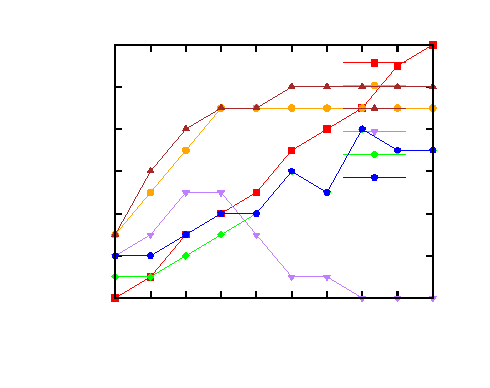
\includegraphics{bounds_epslatex/bounds_5_density_vs_value}}%
    \gplfronttext
  \end{picture}%
\endgroup

	\setcaptionwidth{5cm}
	\caption{Valores de las cotas para $n = 5$.}
	\label{fig:valores_5x5}
\end{minipage}%
\hfill%
\begin{minipage}[t]{0.45\textwidth}
	\centering
	% GNUPLOT: LaTeX picture with Postscript
\begingroup
  \makeatletter
  \providecommand\color[2][]{%
    \GenericError{(gnuplot) \space\space\space\@spaces}{%
      Package color not loaded in conjunction with
      terminal option `colourtext'%
    }{See the gnuplot documentation for explanation.%
    }{Either use 'blacktext' in gnuplot or load the package
      color.sty in LaTeX.}%
    \renewcommand\color[2][]{}%
  }%
  \providecommand\includegraphics[2][]{%
    \GenericError{(gnuplot) \space\space\space\@spaces}{%
      Package graphicx or graphics not loaded%
    }{See the gnuplot documentation for explanation.%
    }{The gnuplot epslatex terminal needs graphicx.sty or graphics.sty.}%
    \renewcommand\includegraphics[2][]{}%
  }%
  \providecommand\rotatebox[2]{#2}%
  \@ifundefined{ifGPcolor}{%
    \newif\ifGPcolor
    \GPcolorfalse
  }{}%
  \@ifundefined{ifGPblacktext}{%
    \newif\ifGPblacktext
    \GPblacktexttrue
  }{}%
  % define a \g@addto@macro without @ in the name:
  \let\gplgaddtomacro\g@addto@macro
  % define empty templates for all commands taking text:
  \gdef\gplbacktext{}%
  \gdef\gplfronttext{}%
  \makeatother
  \ifGPblacktext
    % no textcolor at all
    \def\colorrgb#1{}%
    \def\colorgray#1{}%
  \else
    % gray or color?
    \ifGPcolor
      \def\colorrgb#1{\color[rgb]{#1}}%
      \def\colorgray#1{\color[gray]{#1}}%
      \expandafter\def\csname LTw\endcsname{\color{white}}%
      \expandafter\def\csname LTb\endcsname{\color{black}}%
      \expandafter\def\csname LTa\endcsname{\color{black}}%
      \expandafter\def\csname LT0\endcsname{\color[rgb]{1,0,0}}%
      \expandafter\def\csname LT1\endcsname{\color[rgb]{0,1,0}}%
      \expandafter\def\csname LT2\endcsname{\color[rgb]{0,0,1}}%
      \expandafter\def\csname LT3\endcsname{\color[rgb]{1,0,1}}%
      \expandafter\def\csname LT4\endcsname{\color[rgb]{0,1,1}}%
      \expandafter\def\csname LT5\endcsname{\color[rgb]{1,1,0}}%
      \expandafter\def\csname LT6\endcsname{\color[rgb]{0,0,0}}%
      \expandafter\def\csname LT7\endcsname{\color[rgb]{1,0.3,0}}%
      \expandafter\def\csname LT8\endcsname{\color[rgb]{0.5,0.5,0.5}}%
    \else
      % gray
      \def\colorrgb#1{\color{black}}%
      \def\colorgray#1{\color[gray]{#1}}%
      \expandafter\def\csname LTw\endcsname{\color{white}}%
      \expandafter\def\csname LTb\endcsname{\color{black}}%
      \expandafter\def\csname LTa\endcsname{\color{black}}%
      \expandafter\def\csname LT0\endcsname{\color{black}}%
      \expandafter\def\csname LT1\endcsname{\color{black}}%
      \expandafter\def\csname LT2\endcsname{\color{black}}%
      \expandafter\def\csname LT3\endcsname{\color{black}}%
      \expandafter\def\csname LT4\endcsname{\color{black}}%
      \expandafter\def\csname LT5\endcsname{\color{black}}%
      \expandafter\def\csname LT6\endcsname{\color{black}}%
      \expandafter\def\csname LT7\endcsname{\color{black}}%
      \expandafter\def\csname LT8\endcsname{\color{black}}%
    \fi
  \fi
  \setlength{\unitlength}{0.0500bp}%
  \begin{picture}(4392.00,3400.00)%
    \gplgaddtomacro\gplbacktext{%
      \csname LTb\endcsname%
      \put(814,704){\makebox(0,0)[r]{\strut{} 0}}%
      \put(814,1109){\makebox(0,0)[r]{\strut{} 10}}%
      \put(814,1514){\makebox(0,0)[r]{\strut{} 20}}%
      \put(814,1920){\makebox(0,0)[r]{\strut{} 30}}%
      \put(814,2325){\makebox(0,0)[r]{\strut{} 40}}%
      \put(814,2730){\makebox(0,0)[r]{\strut{} 50}}%
      \put(814,3135){\makebox(0,0)[r]{\strut{} 60}}%
      \put(946,484){\makebox(0,0){\strut{} 10}}%
      \put(1285,484){\makebox(0,0){\strut{} 20}}%
      \put(1624,484){\makebox(0,0){\strut{} 30}}%
      \put(1962,484){\makebox(0,0){\strut{} 40}}%
      \put(2301,484){\makebox(0,0){\strut{} 50}}%
      \put(2640,484){\makebox(0,0){\strut{} 60}}%
      \put(2979,484){\makebox(0,0){\strut{} 70}}%
      \put(3317,484){\makebox(0,0){\strut{} 80}}%
      \put(3656,484){\makebox(0,0){\strut{} 90}}%
      \put(3995,484){\makebox(0,0){\strut{} 100}}%
      \put(176,1919){\rotatebox{-270}{\makebox(0,0){\strut{}Valor de la funci\'on}}}%
      \put(2470,154){\makebox(0,0){\strut{}Porcentaje de clientes ($p$)}}%
    }%
    \gplgaddtomacro\gplfronttext{%
      \csname LTb\endcsname%
      \put(3008,2962){\makebox(0,0)[r]{\strut{}\texttt{clients\_count}}}%
      \csname LTb\endcsname%
      \put(3008,2742){\makebox(0,0)[r]{\strut{}\texttt{dist\_x2}}}%
      \csname LTb\endcsname%
      \put(3008,2522){\makebox(0,0)[r]{\strut{}\texttt{dist\_x3}}}%
      \csname LTb\endcsname%
      \put(3008,2302){\makebox(0,0)[r]{\strut{}\texttt{mst}}}%
      \csname LTb\endcsname%
      \put(3008,2082){\makebox(0,0)[r]{\strut{}\texttt{vc}}}%
      \csname LTb\endcsname%
      \put(3008,1862){\makebox(0,0)[r]{\strut{}\texttt{vc\_mst}}}%
    }%
    \gplbacktext
    \put(0,0){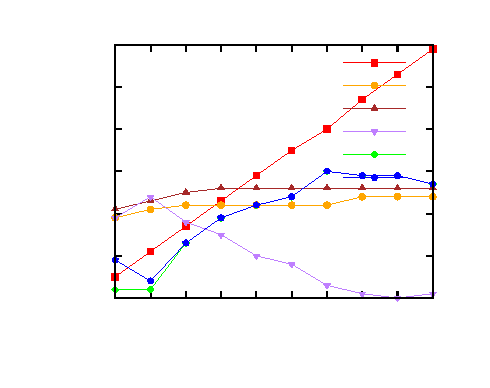
\includegraphics{bounds_epslatex/bounds_10_density_vs_value}}%
    \gplfronttext
  \end{picture}%
\endgroup

	\setcaptionwidth{5cm}
    \caption{Valores de las cotas para $n = 10$.}
	\label{fig:valores_10x10}
\end{minipage}

\begin{minipage}[t]{0.45\textwidth}
	\centering
	% GNUPLOT: LaTeX picture with Postscript
\begingroup
  \makeatletter
  \providecommand\color[2][]{%
    \GenericError{(gnuplot) \space\space\space\@spaces}{%
      Package color not loaded in conjunction with
      terminal option `colourtext'%
    }{See the gnuplot documentation for explanation.%
    }{Either use 'blacktext' in gnuplot or load the package
      color.sty in LaTeX.}%
    \renewcommand\color[2][]{}%
  }%
  \providecommand\includegraphics[2][]{%
    \GenericError{(gnuplot) \space\space\space\@spaces}{%
      Package graphicx or graphics not loaded%
    }{See the gnuplot documentation for explanation.%
    }{The gnuplot epslatex terminal needs graphicx.sty or graphics.sty.}%
    \renewcommand\includegraphics[2][]{}%
  }%
  \providecommand\rotatebox[2]{#2}%
  \@ifundefined{ifGPcolor}{%
    \newif\ifGPcolor
    \GPcolorfalse
  }{}%
  \@ifundefined{ifGPblacktext}{%
    \newif\ifGPblacktext
    \GPblacktexttrue
  }{}%
  % define a \g@addto@macro without @ in the name:
  \let\gplgaddtomacro\g@addto@macro
  % define empty templates for all commands taking text:
  \gdef\gplbacktext{}%
  \gdef\gplfronttext{}%
  \makeatother
  \ifGPblacktext
    % no textcolor at all
    \def\colorrgb#1{}%
    \def\colorgray#1{}%
  \else
    % gray or color?
    \ifGPcolor
      \def\colorrgb#1{\color[rgb]{#1}}%
      \def\colorgray#1{\color[gray]{#1}}%
      \expandafter\def\csname LTw\endcsname{\color{white}}%
      \expandafter\def\csname LTb\endcsname{\color{black}}%
      \expandafter\def\csname LTa\endcsname{\color{black}}%
      \expandafter\def\csname LT0\endcsname{\color[rgb]{1,0,0}}%
      \expandafter\def\csname LT1\endcsname{\color[rgb]{0,1,0}}%
      \expandafter\def\csname LT2\endcsname{\color[rgb]{0,0,1}}%
      \expandafter\def\csname LT3\endcsname{\color[rgb]{1,0,1}}%
      \expandafter\def\csname LT4\endcsname{\color[rgb]{0,1,1}}%
      \expandafter\def\csname LT5\endcsname{\color[rgb]{1,1,0}}%
      \expandafter\def\csname LT6\endcsname{\color[rgb]{0,0,0}}%
      \expandafter\def\csname LT7\endcsname{\color[rgb]{1,0.3,0}}%
      \expandafter\def\csname LT8\endcsname{\color[rgb]{0.5,0.5,0.5}}%
    \else
      % gray
      \def\colorrgb#1{\color{black}}%
      \def\colorgray#1{\color[gray]{#1}}%
      \expandafter\def\csname LTw\endcsname{\color{white}}%
      \expandafter\def\csname LTb\endcsname{\color{black}}%
      \expandafter\def\csname LTa\endcsname{\color{black}}%
      \expandafter\def\csname LT0\endcsname{\color{black}}%
      \expandafter\def\csname LT1\endcsname{\color{black}}%
      \expandafter\def\csname LT2\endcsname{\color{black}}%
      \expandafter\def\csname LT3\endcsname{\color{black}}%
      \expandafter\def\csname LT4\endcsname{\color{black}}%
      \expandafter\def\csname LT5\endcsname{\color{black}}%
      \expandafter\def\csname LT6\endcsname{\color{black}}%
      \expandafter\def\csname LT7\endcsname{\color{black}}%
      \expandafter\def\csname LT8\endcsname{\color{black}}%
    \fi
  \fi
  \setlength{\unitlength}{0.0500bp}%
  \begin{picture}(4392.00,3400.00)%
    \gplgaddtomacro\gplbacktext{%
      \csname LTb\endcsname%
      \put(946,704){\makebox(0,0)[r]{\strut{} 0}}%
      \put(946,1109){\makebox(0,0)[r]{\strut{} 100}}%
      \put(946,1514){\makebox(0,0)[r]{\strut{} 200}}%
      \put(946,1920){\makebox(0,0)[r]{\strut{} 300}}%
      \put(946,2325){\makebox(0,0)[r]{\strut{} 400}}%
      \put(946,2730){\makebox(0,0)[r]{\strut{} 500}}%
      \put(946,3135){\makebox(0,0)[r]{\strut{} 600}}%
      \put(1078,484){\makebox(0,0){\strut{} 10}}%
      \put(1402,484){\makebox(0,0){\strut{} 20}}%
      \put(1726,484){\makebox(0,0){\strut{} 30}}%
      \put(2050,484){\makebox(0,0){\strut{} 40}}%
      \put(2374,484){\makebox(0,0){\strut{} 50}}%
      \put(2699,484){\makebox(0,0){\strut{} 60}}%
      \put(3023,484){\makebox(0,0){\strut{} 70}}%
      \put(3347,484){\makebox(0,0){\strut{} 80}}%
      \put(3671,484){\makebox(0,0){\strut{} 90}}%
      \put(3995,484){\makebox(0,0){\strut{} 100}}%
      \put(176,1919){\rotatebox{-270}{\makebox(0,0){\strut{}Valor de la funci\'on}}}%
      \put(2536,154){\makebox(0,0){\strut{}Porcentaje de clientes ($p$)}}%
    }%
    \gplgaddtomacro\gplfronttext{%
      \csname LTb\endcsname%
      \put(3008,2962){\makebox(0,0)[r]{\strut{}\texttt{clients\_count}}}%
      \csname LTb\endcsname%
      \put(3008,2742){\makebox(0,0)[r]{\strut{}\texttt{dist\_x2}}}%
      \csname LTb\endcsname%
      \put(3008,2522){\makebox(0,0)[r]{\strut{}\texttt{dist\_x3}}}%
      \csname LTb\endcsname%
      \put(3008,2302){\makebox(0,0)[r]{\strut{}\texttt{mst}}}%
      \csname LTb\endcsname%
      \put(3008,2082){\makebox(0,0)[r]{\strut{}\texttt{vc}}}%
      \csname LTb\endcsname%
      \put(3008,1862){\makebox(0,0)[r]{\strut{}\texttt{vc\_mst}}}%
    }%
    \gplbacktext
    \put(0,0){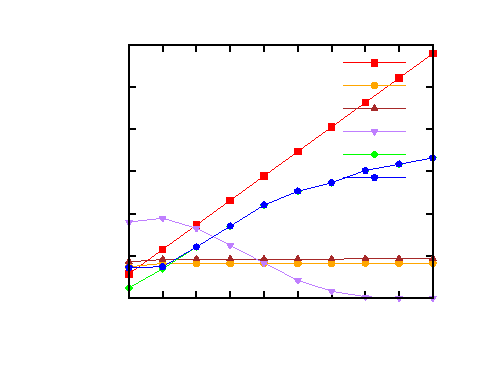
\includegraphics{bounds_epslatex/bounds_30_density_vs_value}}%
    \gplfronttext
  \end{picture}%
\endgroup

	\setcaptionwidth{5cm}
	\caption{Valores de las cotas para $n = 30$.}
	\label{fig:valores_30x30}
\end{minipage}%
\hfill%
\begin{minipage}[t]{0.45\textwidth}
	\centering
	% GNUPLOT: LaTeX picture with Postscript
\begingroup
  \makeatletter
  \providecommand\color[2][]{%
    \GenericError{(gnuplot) \space\space\space\@spaces}{%
      Package color not loaded in conjunction with
      terminal option `colourtext'%
    }{See the gnuplot documentation for explanation.%
    }{Either use 'blacktext' in gnuplot or load the package
      color.sty in LaTeX.}%
    \renewcommand\color[2][]{}%
  }%
  \providecommand\includegraphics[2][]{%
    \GenericError{(gnuplot) \space\space\space\@spaces}{%
      Package graphicx or graphics not loaded%
    }{See the gnuplot documentation for explanation.%
    }{The gnuplot epslatex terminal needs graphicx.sty or graphics.sty.}%
    \renewcommand\includegraphics[2][]{}%
  }%
  \providecommand\rotatebox[2]{#2}%
  \@ifundefined{ifGPcolor}{%
    \newif\ifGPcolor
    \GPcolorfalse
  }{}%
  \@ifundefined{ifGPblacktext}{%
    \newif\ifGPblacktext
    \GPblacktexttrue
  }{}%
  % define a \g@addto@macro without @ in the name:
  \let\gplgaddtomacro\g@addto@macro
  % define empty templates for all commands taking text:
  \gdef\gplbacktext{}%
  \gdef\gplfronttext{}%
  \makeatother
  \ifGPblacktext
    % no textcolor at all
    \def\colorrgb#1{}%
    \def\colorgray#1{}%
  \else
    % gray or color?
    \ifGPcolor
      \def\colorrgb#1{\color[rgb]{#1}}%
      \def\colorgray#1{\color[gray]{#1}}%
      \expandafter\def\csname LTw\endcsname{\color{white}}%
      \expandafter\def\csname LTb\endcsname{\color{black}}%
      \expandafter\def\csname LTa\endcsname{\color{black}}%
      \expandafter\def\csname LT0\endcsname{\color[rgb]{1,0,0}}%
      \expandafter\def\csname LT1\endcsname{\color[rgb]{0,1,0}}%
      \expandafter\def\csname LT2\endcsname{\color[rgb]{0,0,1}}%
      \expandafter\def\csname LT3\endcsname{\color[rgb]{1,0,1}}%
      \expandafter\def\csname LT4\endcsname{\color[rgb]{0,1,1}}%
      \expandafter\def\csname LT5\endcsname{\color[rgb]{1,1,0}}%
      \expandafter\def\csname LT6\endcsname{\color[rgb]{0,0,0}}%
      \expandafter\def\csname LT7\endcsname{\color[rgb]{1,0.3,0}}%
      \expandafter\def\csname LT8\endcsname{\color[rgb]{0.5,0.5,0.5}}%
    \else
      % gray
      \def\colorrgb#1{\color{black}}%
      \def\colorgray#1{\color[gray]{#1}}%
      \expandafter\def\csname LTw\endcsname{\color{white}}%
      \expandafter\def\csname LTb\endcsname{\color{black}}%
      \expandafter\def\csname LTa\endcsname{\color{black}}%
      \expandafter\def\csname LT0\endcsname{\color{black}}%
      \expandafter\def\csname LT1\endcsname{\color{black}}%
      \expandafter\def\csname LT2\endcsname{\color{black}}%
      \expandafter\def\csname LT3\endcsname{\color{black}}%
      \expandafter\def\csname LT4\endcsname{\color{black}}%
      \expandafter\def\csname LT5\endcsname{\color{black}}%
      \expandafter\def\csname LT6\endcsname{\color{black}}%
      \expandafter\def\csname LT7\endcsname{\color{black}}%
      \expandafter\def\csname LT8\endcsname{\color{black}}%
    \fi
  \fi
  \setlength{\unitlength}{0.0500bp}%
  \begin{picture}(4392.00,3400.00)%
    \gplgaddtomacro\gplbacktext{%
      \csname LTb\endcsname%
      \put(1078,704){\makebox(0,0)[r]{\strut{} 0}}%
      \put(1078,974){\makebox(0,0)[r]{\strut{} 200}}%
      \put(1078,1244){\makebox(0,0)[r]{\strut{} 400}}%
      \put(1078,1514){\makebox(0,0)[r]{\strut{} 600}}%
      \put(1078,1784){\makebox(0,0)[r]{\strut{} 800}}%
      \put(1078,2055){\makebox(0,0)[r]{\strut{} 1000}}%
      \put(1078,2325){\makebox(0,0)[r]{\strut{} 1200}}%
      \put(1078,2595){\makebox(0,0)[r]{\strut{} 1400}}%
      \put(1078,2865){\makebox(0,0)[r]{\strut{} 1600}}%
      \put(1078,3135){\makebox(0,0)[r]{\strut{} 1800}}%
      \put(1210,484){\makebox(0,0){\strut{} 10}}%
      \put(1519,484){\makebox(0,0){\strut{} 20}}%
      \put(1829,484){\makebox(0,0){\strut{} 30}}%
      \put(2138,484){\makebox(0,0){\strut{} 40}}%
      \put(2448,484){\makebox(0,0){\strut{} 50}}%
      \put(2757,484){\makebox(0,0){\strut{} 60}}%
      \put(3067,484){\makebox(0,0){\strut{} 70}}%
      \put(3376,484){\makebox(0,0){\strut{} 80}}%
      \put(3686,484){\makebox(0,0){\strut{} 90}}%
      \put(3995,484){\makebox(0,0){\strut{} 100}}%
      \put(176,1919){\rotatebox{-270}{\makebox(0,0){\strut{}Valor de la funci\'on}}}%
      \put(2602,154){\makebox(0,0){\strut{}Porcentaje de clientes ($p$)}}%
    }%
    \gplgaddtomacro\gplfronttext{%
      \csname LTb\endcsname%
      \put(3008,2962){\makebox(0,0)[r]{\strut{}\texttt{clients\_count}}}%
      \csname LTb\endcsname%
      \put(3008,2742){\makebox(0,0)[r]{\strut{}\texttt{dist\_x2}}}%
      \csname LTb\endcsname%
      \put(3008,2522){\makebox(0,0)[r]{\strut{}\texttt{mst}}}%
      \csname LTb\endcsname%
      \put(3008,2302){\makebox(0,0)[r]{\strut{}\texttt{vc}}}%
      \csname LTb\endcsname%
      \put(3008,2082){\makebox(0,0)[r]{\strut{}\texttt{vc\_mst}}}%
    }%
    \gplbacktext
    \put(0,0){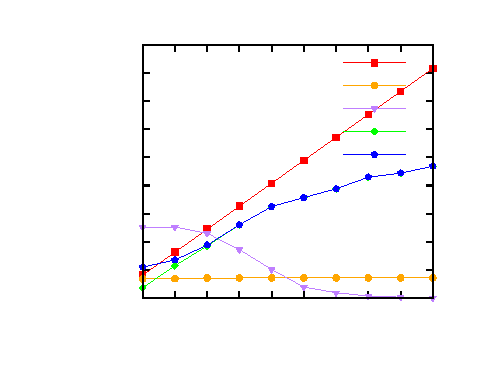
\includegraphics{bounds_epslatex/bounds_50_density_vs_value}}%
    \gplfronttext
  \end{picture}%
\endgroup

	\setcaptionwidth{5cm}
    \caption{Valores de las cotas para $n = 50$.}
	\label{fig:valores_50x50}
\end{minipage}
\end{figure}

\clearpage

La primera conclusi'on que se puede sacar es que las mediciones (tanto de tiempo de ejecuci'on como de valor de las cotas) convergen a medida que $n$ crece, lo cual se observa en la tendencia de los resultados para $n = 10, 30$ y  $50$. Lo segundo que se observa es que los resultados para $n = 5$ no siguen el patr'on general, lo cual es razonable, debido a que las instancias de ese tama\~no son demasiado chicas. En lo que sigue, s'olo analizamos los resultados para $n = 10, 30$ y $50$.

En todos los casos, la cota m'as costosa es \texttt{dist\_x3}, que insume tres o m'as 'ordenes de magnitud m'as de tiempo que el resto de las cotas. Dejamos de lado esta cota para analizar y comparar el resto. Se puede ver todas las cotas mantienen, aproximado, el mismo orden relativo a medida que $p$ crece, excepto por \texttt{vc\_mst}, que comienza siendo la m'as costosa pero es superada por \texttt{dist\_x2} y \texttt{mst}. La \autoref{ta:rankings_tiempos} muestra el ranking aproximado de cotas, por tiempos de ejecuci'on, seg'un indica la tendencia general. Para construir este ranking particionamos la escala de porcentajes en tres intervalos, $[10, 30)$, $[30, 50)$ y $[50, 100]$, elegidos en base a las variaciones de costo y efectividad que observamos en los gr'aficos. En cada intervalo, el ranking de cada cota est'a dado por una estimaci'on del 'area debajo de su curva, de la \autoref{fig:tiempos_30x30}.

\begin{table}[h]
\begin{center}
\begin{tabular}{|c|c|c|c|c|}
\hline
\# & $p \in [10, 30)$ & $p \in [30, 50)$ & $p \in [50, 100]$\\
\hline
1 & \texttt{dist\_x3} & \texttt{dist\_x3} & \texttt{dist\_x3}\\
2 & \texttt{vc\_mst} & \texttt{vc\_mst} & \texttt{dist\_x2} (+1)\\
3 & \texttt{dist\_x2} & \texttt{dist\_x2} & \texttt{mst} (+1)\\
4 & \texttt{mst} & \texttt{mst} & \texttt{vc\_mst} (-2)\\
5 & \texttt{vc} & \texttt{vc} & \texttt{vc}\\
6 & \texttt{clients\_count} & \texttt{clients\_count} & \texttt{clients\_count}\\
\hline
\end{tabular}
\end{center}
\caption{Ranking aproximado de cotas, por tiempo de ejecuci'on.}
\label{ta:rankings_tiempos}
\end{table}

Elaboramos el mismo ranking aproximado para la efectividad de las cotas, que se muestra en la \autoref{ta:rankings_valores}. En este caso, confeccionamos el ranking en base a la \autoref{fig:valores_30x30}. Hay varias observaciones interesantes a hacer sobre la efectividad registrada de las cotas. En primer lugar, es notable que la cota \texttt{clients\_count}, la m'as simple de calcular de todas, sea la m'as efectiva, por una diferencia importante, para $p \in [30, 100]$. En segundo lugar, se puede ver que \texttt{vc} y \texttt{vc\_mst} convergen r'apidamente al (aproximadamente) mismo valor, a medida que $p$ crece. Esto se debe, presumiblemente, a que a mayor densidad de clientes, las componentes conexas de $G[X]$ est'an una m'as cerca de la otra, en $G$, lo que se traduce en que $\mst(H, \dist)$ tiende a $r - 1$, y por ende el t'ermino $\mst(H, \dist) - (r - 1)$ de \texttt{vc\_mst} tiende a $0$. En tercer lugar, se puede ver que la diferencia entre \texttt{dist\_x2} y \texttt{dist\_x3} es muy peque\~na, con lo cual se puede concluir que, en general, no tiene mucho sentido usar \texttt{dist\_x3}, que tiene un tiempo de ejecuci'on 'ordenes de magnitud m'as grande. Para terminar, hacemos una menci'on al comportamiento de \texttt{mst}, que es la 'unica cota que decrece a medida que $p$ crece. Esto se explica del mismo modo que la convergencia de \texttt{vc} y \texttt{vc\_mst} al mismo valor: a medida que la densidad de clientes crece, la distancia entre los clientes decrece, y por ende $\mst(K(X), \dist)$ tiende a $0$.

\begin{table}[h]
\begin{center}
\begin{tabular}{|c|c|c|c|c|}
\hline
\# & $p \in [10, 30)$ & $p \in [30, 50)$ & $p \in [50, 100]$\\
\hline
1 & \texttt{mst} & \texttt{clients\_count} (+1) & \texttt{clients\_count}\\
2 & \texttt{clients\_count} & \texttt{vc\_mst} (+2) & \texttt{vc\_mst}\\
3 & \texttt{dist\_x3} & \texttt{vc} (+3) & \texttt{vc}\\
4 & \texttt{vc\_mst} & \texttt{mst} (-3) & \texttt{dist\_x3} (+1)\\
5 & \texttt{dist\_x2} & \texttt{dist\_x3} (-2) & \texttt{dist\_x2} (+1)\\
6 & \texttt{vc} & \texttt{dist\_x2} (-1) & \texttt{mst} (-2)\\
\hline
\end{tabular}
\end{center}
\caption{Ranking aproximado de cotas, por valor.}
\label{ta:rankings_valores}
\end{table}

Enumeramos a continuaci'on algunas conclusiones surgidas de la experimentaci'on:

\begin{itemize}
\item En general, \texttt{dist\_x2} es un buen sustituto de \texttt{dist\_x3}, y \texttt{vc} lo es de \texttt{vc\_mst}.

\item Como \texttt{clients\_count} toma unos pocos milisegundos, siempre conviene ejecutarla, y en primer lugar.

\item Para $p \geq 30$, \texttt{clients\_count} es la cota m'as efectiva, seguida de \texttt{vc}. Como adem'as, estas dos cotas son las que menos tiempo insumen, son indiscutiblemente la mejor opci'on.

\item Para $p < 30$, \texttt{mst} es la cota m'as efectiva, seguida de \texttt{clients\_count}, y sus costos confirman que, son una excelente elecci'on.

\item En grillas muy peque\~nas (del orden de $5 \times 5$), las conclusiones anteriores no son v'alidas. En estos casos, la mejor opci'on pareciera ser \texttt{dist\_x2}, tanto por su efectividad como por su costo.
\end{itemize}

En base a estas conclusiones, confeccionamos una funci'on \textsc{Prune}, que se presenta en el \autoref{al:prune_grillas_tuneado}.

\begin{algorithm}
  \caption{Aplicaci'on de las funciones de acotaci'on, sobre grillas.}
  \label{al:prune_grillas_tuneado}
  \begin{algorithmic}[1]
  	\Require El v'ertice actual $u$, el conjunto $F$ de clientes que resta cubrir, y la longitud $\ell$ del camino recorrido hasta $u$.
  	\Ensure \True si alguna funci'on de acotaci'on indica que el camino recorrido no podr'a mejorar $opt\_length$, y \False en caso contrario.
	\Function{Prune}{$u, F, \ell$}
	\State Sean $n$ y $m$ las dimensiones de la grilla.
	\State $M \gets n(m - 1) + m(n - 1)$ \Comment{la cantidad de aristas de la grilla}
	\State $p \gets |F| / M$
	\If{$M < 80$} \Comment{la grilla es, aproximadamente, de $7 \times 7$ o m'as chica}
		\If{$\ell + \texttt{dist\_x2}(u, F) \geq opt\_length$}
			\Return \True
		\EndIf
	\Else
		\If{$0.3 \leq p$ \And ($\ell + \texttt{clients\_count}(F) \geq opt\_length$ \Or $\ell + \texttt{vc}(F) \geq opt\_length$)}
			\Return \True
		\ElsIf{$p < 0.3$ \And ($\ell + \texttt{clients\_count}(F) \geq opt\_length$ \Or $\ell + \texttt{mst}(F) \geq opt\_length$)}
			\Return \True
		\EndIf
	\EndIf
	\Return \False
	\EndFunction
  \end{algorithmic}
\end{algorithm}

\subsection{Algoritmos exactos}

\label{su:experimentacion_algoritmos_exactos}

En lo que sigue, llamamos \textit{algoritmo BT} al algoritmo de backtracking y \textit{algoritmo PD} al algoritmo de programaci'on din'amica. Las implementaciones de los estos algoritmos no ofrecen mayores dificultades t'ecnicas. Debemos mencionar que en la del algoritmo PD utilizamos \texttt{std::map} para implementar los diccionarios. Esta clase de la biblioteca est'andar de C++ es la representaci'on de un diccionario como un 'arbol binario de b'usqueda balanceado \cite{Pl00}. En ambos algoritmos, implementamos el subconjunto de clientes $F$ con un \texttt{std::set}, que usa la misma estructura interna que \texttt{std::map}. Si bien en el an'alisis previo asumimos que $F$ realiza inserciones, borrado y consulta en $O(1)$, una representaci'on de \texttt{std::map} respeta, a nivel pr'actico, estos costos temporales, pues la cantidad de clientes que manejamos es peque\~na.

Como los dos algoritmos exactos corren en tiempo supra-polinomial en la cantidad $k$ de clientes, es esperable que s'olo sean capaces de resolver instancias de pocos clientes. Para tener una idea de cu'al es la eficiencia esperable, en tiempo y espacio, de nuestros algoritmos, calculamos algunos valores puntuales de las estimaciones asint'oticas de las complejidades temporal y espacial, y los presentamos en la \autoref{ta:algoritmos_tiempo_espacio}. L'ogicamente, estos n'umeros no deben interpretarse en forma absoluta, pues los c'alculos asint'oticos esconden constantes y t'erminos que aportan al costo total. Para analizar la tabla, tengamos en mente que un procesador \textit{commodity} moderno ejecuta alrededor de $10^9$ (mil millones) de instrucciones por segundo, y que los experimentos se ejecutaron sobre una computadora con alrededor de $8GB$ de RAM. En funci'on de estos datos, podemos plantear algunas tesis previas a la experimentaci'on:

\begin{itemize}
	\item El algoritmo BT no podr'a ejecutar instancias de m'as de $15$ clientes, en una cantidad de tiempo razonable (del orden de unas pocas horas), a menos que las funciones de acotaci'on reduzcan el c'omputo necesario.
	\item El algoritmo PD no podr'a ejecutar instancias de m'as de $20$ clientes, en una computadora con una cantidad de memoria razonable (del orden de unos pocos $GB$), a menos que las funciones de acotaci'on reduzcan el c'omputo necesario.
\end{itemize}

\begin{table}[h]
\begin{center}
\begin{tabular}{|c|c|c|c|c|}
\hline
$k$ & Tiempo BT & Tiempo PD & Espacio PD & Instancias\\
 & $k \cdot k!$ & $k^4 2^k$ & $k^2 2^k$ & $(n, p)$\\
\hline
$5$ & $0.6 \cdot 10^3$ & $20 \cdot 10^3$ & $0.8k$ & $(5, 10)$\\
$10$ & $\sim 36 \cdot 10^6$ & $\sim 10 \cdot 10^6$ & $\sim 100k$ & $(5, 20)$, $(5, 30)$\\
$15$ & $\sim 19 \cdot 10^{12}$ & $\sim 1.6 \cdot 10^9$ & $\sim 7M$ & $(5, 40)$\\
$20$ & $\sim 48 \cdot 10^{18}$ & $\sim 167 \cdot 10^9$ & $\sim 419M$ & $(5, 50)$, $(10, 10)$\\
$25$ & $\sim 387 \cdot 10^{24}$ & $\sim 13 \cdot 10^{12}$ & $\sim 20G$ & $(5, 60)$\\
$30$ & $\sim 8 \cdot 10^{33}$ & $\sim 869 \cdot 10^{12}$ & $\sim 966G$ & $(5, 70)$\\
$35$ & - & - & - & $(10, 20)$\\
$40$ & - & - & - & $(15, 10)$\\
\hline
\end{tabular}
\end{center}
\caption{Estimaciones de requerimientos de tiempo y espacio de los algoritmos de backtracking (BT) y de programaci'on din'amica (PD). La columna de instancias enumera los par'ametros de instancias con aproximadamente la cantidad de clientes de cada l'inea.}
\label{ta:algoritmos_tiempo_espacio}
\end{table}

Corrimos las implementaciones de los dos algoritmos exactos con las funciones de acotaci'on, y medimos el tiempo de ejecuci'on en cada caso. Cada instancia se ejecut'o durante $1$ hora, y cumplido ese plazo se detuvo la ejecuci'on. Se comprob'o que a'un utilizando funciones de acotaci'on para acelerar el c'omputo, los algoritmos exactos s'olo pueden resolver instancias de $25$ o menos clientes en la ventana de tiempo provista. Presentamos los resultados en la \autoref{ta:tiempos_bt} y \autoref{ta:tiempos_dp}. Estas tablas presentan los tiempos de ejecuci'on de los dos algoritmos exactos, con y sin funciones de acotaci'on, para las instancias que completaron su ejecuci'on en menos de $1$ hora. A las ejecuciones que sufrieron detenciones forzosas por excederse del l'imite de $1$ hora, las simbolizamos \textit{TLE} (por sus siglas en ingl'es, \textit{time-limit exceeded}).

\begin{table}[h]
\centering
\begin{tabular}{|c|c|c|c|}
\hline
$n$ & $p$ & Tiempo BT sin cotas (seg) & Tiempo BT con cotas (seg)\\
\hline
$5$ & $10$ & $\sim 10^{-5}$ & $\sim 10^{-5}$\\
$5$ & $20$ & $\sim 0.01$ & $\sim 10^{-4}$\\
$5$ & $30$ & $\sim 200$ & $\sim 0.01$\\
$5$ & $40$ & TLE & $\sim 0.1$\\
$5$ & $50$ & TLE & $\sim 9$\\
$5$ & $60$ & TLE & $\sim 2700$\\
$10$ & $10$ & TLE & $\sim 3.5$\\
\hline
\end{tabular}
\caption{Tiempos de ejecuci'on para el algoritmo BT.}
\label{ta:tiempos_bt}
\hfill \\
\begin{tabular}{|c|c|c|c|}
\hline
$n$ & $p$ & Tiempo PD sin cotas (seg) & Tiempo PD con cotas (seg)\\
\hline
$5$ & $10$ & $\sim 10^{-4}$ & $\sim 10^{-4}$\\
$5$ & $20$ & $\sim 0.01$ & $\sim 0.01$\\
$5$ & $30$ & $\sim 1$ & $\sim 0.1$\\
$5$ & $40$ & $\sim 55$ & $\sim 20$\\
$10$ & $10$ & TLE & $\sim 175$\\
\hline
\end{tabular}
\caption{Tiempos de ejecuci'on para el algoritmo PD.}
\label{ta:tiempos_dp}
\end{table}

Se puede ver que las cotas hacen un buen trabajo disminuyendo el tiempo de ejecuci'on. Por ejemplo, la instancia $(n, p) = (5, 30)$ toma aproximadamente $200$ segundos para ser ejecutada por el algoritmo BT sin cotas, y apenas $0.01$ segundo para ese mismo algoritmo pero con cotas. Se pueden observar an'alogas, aunque menores, reducciones en los tiempos del algoritmo PD. En ambos casos, se puede observar que al utilizar las cotas, los algoritmos logran ejecutar, en el tiempo provisto, instancias que no terminan de correr de otro modo.

Lamentablemente, el buen trabajo de las cotas no es suficiente para que estos algoritmos logren ejecutar, en un tiempo razonable, instancias de tama\~no real, del orden de las decenas y cientos de clientes.

Como \textsc{Prune} utiliza 'unicamente la cota \texttt{dist\_x2} para instancias de $n = 5$, es necesaria una experimentaci'on con una ventana de tiempo m'as grande, de varias horas, para medir con precisi'on el trabajo de las dem'as cotas, cuyos buenos resultados s'olo pudimos apreciar en las dos instancias de $n = 10$ que lograron terminar su ejecuci'on.
\cleardoublepage
\chapter{Algoritmos aproximados para \problem{STAR ROUTING}}
\label{ch:aproximados}
%{\begin{small}%
%\begin{flushright}%
%\it
%No! No different! Only different in your mind.\\
%--Maestro Yoda
%\end{flushright}%
%\end{small}%
%\vspace{.5cm}}

Recordemos que un algoritmo aproximado es un algoritmo que produce soluciones factibles para un problema, pero que no necesariamente son 'optimas. En este cap'itulo presentamos una variedad de algoritmos aproximados para \problem{SR} sobre distintas clases de grafos: general, sobre grillas y sobre grafos completos. El estudio de la existencia de algoritmos aproximados para un problema es interesante tanto desde el punto de vista te'orico como pr'actico. Por un lado, es interesante desde lo te'orico, porque la mera existencia o no de algoritmos aproximados para un problema habla sobre su grado de dificultad. Por ejemplo, es bien sabido que \problem{TSP} no admite algoritmos aproximados con factor de aproximaci'on constante \cite[p. 147]{Ga76}, mientras que para \problem{TSP} m'etrico hay un algoritmo $(3/2)$-aproximado \cite[p. 132]{Ga76}, por lo que podemos decir que la versi'on m'etrica es ``m'as f'acil'', a'un cuando no se conocen algoritmos eficientes para ninguno de los dos problemas. Desde el punto de vista pr'actico, un algoritmo aproximado es un buen m'etodo para generar una soluci'on factible inicial en el contexto de un algoritmo exacto. Si el factor de aproximaci'on es peque\~no, tenemos la garant'ia de que dicha soluci'on factible no est'a demasiado lejos de la soluci'on 'optima. Combinando esto con buenas funciones de acotaci'on podemos acelerar radicalmente la exploraci'on del espacio de soluciones.

Durante este cap'itulo, $(G, X)$ es una instancia de \problem{SR} y escribimos $Z = \problem{SR}^*(G, X)$ y $k = |X|$.

\section{Relaci'on matem'atica entre \problem{SR} y \problem{PTSP}}

Empezamos explorando ciertas relaciones entre \problem{SR} y \problem{PTSP}. Este an'alisis ser'a 'util posteriormente, pues construiremos aproximaciones para \problem{SR} general y sobre grillas, utilizando algoritmos aproximados para \problem{PTSP} m'etrico y rectil'ineo.

\begin{definition}[Distancia m'axima]
\label{de:distmax}
Dadas dos aristas $e$ y $f$ de un grafo, definimos $\distmax(e, f)$ como la distancia m'as grande entre un extremo de $e$ y uno de $f$. Esto es,

\[\distmax(e, f) = \max\limits_{\substack{u \text{ extremo de }e \\ v \text{ extremo de }f}} \dist(u, v)\]
\end{definition}

\noindent
Notar que $\distmax$ no es una distancia en el sentido matem'atico, porque $\distmax(e, e) = 1 \neq 0$. De todos modos, la denominamos de ese modo, por comodidad. Durante este cap'itulo haremos referencia a una variedad de resultados acerca de $\dist$ sobre aristas y $\distmax$, todos presentados en el \autoref{ch:dist_distmax}.

\begin{lemma}
\label{le:ptsp}
\[\problem{PTSP}^*(K(X), \distmax) \leq \problem{PTSP}^*(K(X), \dist) + 2(k - 1)\]

\begin{proof}
Sea $P = \langle e_1, \dots, e_k \rangle$ una soluci'on 'optima de \problem{PTSP} para $(K(X), \dist)$. Este camino es una soluci'on factible de \problem{PTSP} para la instancia $(K(X), \distmax)$, con lo cual $\problem{PTSP}^*(K(X), \distmax) \leq \length_{\distmax}(P)$. Luego, basta ver que $\length_{\distmax}(P) \leq \problem{PTSP}^*(K(X), \dist) + 2(k - 1)$. Se tiene

\begin{align*}
\length_{\distmax}(P) &= \sum_{i = 1}^{k - 1} \distmax(e_i, e_{i + 1}) &\\
&\leq \sum_{i = 1}^{k - 1} (\dist(e_i, e_{i + 1}) + 2) & \text{(\autoref{le:distmax_leq_dist_plus_2})}\\
&= \sum_{i = 1}^{k - 1} \dist(e_i, e_{i + 1}) + 2(k - 1)&\\
&= \length_{\dist}(P) + 2(k - 1)&\\
&= \problem{PTSP}^*(K(X), \dist) + 2(k - 1)&
\end{align*}
\end{proof}
\end{lemma}

\begin{lemma}
\label{le:ptsp_clients_to_sr}
A partir de una soluci'on factible $P$ de \problem{PTSP} para $(K(X), \dist)$, podemos construir, en tiempo polinomial en el tama\~no de $(G, X)$, una soluci'on factible $Q$ de \problem{SR} para $(G, X)$, tal que $\length(Q) \leq \length_{\distmax}(P)$.

\begin{proof}
Escribamos $P = \langle e_1, \dots, e_k \rangle$. Para cada $1 \leq i \leq k$, sea $u_i$ cualquiera de los extremos de $e_i$. Sea $Q_i$ un camino m'inimo entre $u_i$ y $u_{i + 1}$ en $G$. Definimos $Q = Q_1 \circ \dots \circ Q_{k - 1}$. Se puede ver que esta es una soluci'on factible de \problem{SR} para $(G, X)$. Adem'as

\begin{align*}
\length(Q) &= \sum_{i = 1}^{k - 1} \length(Q_i) &\\
&= \sum_{i = 1}^{k - 1} \dist(u_i, u_{i + 1}) &\\
&\leq \sum_{i = 1}^{k - 1} \distmax(e_i, e_{i + 1}) & \text{(} u_i \text{ es extremo de } e_i \\
& & \text{y } u_{i + 1} \text{ de } e_{i + 1} \text{)}\\
&= \length_{\distmax}(P)
\end{align*}
\end{proof}
\end{lemma}

El siguiente teorema es el primer paso importante, en la comprensi'on de la relaci'on entre \problem{SR} y \problem{PTSP}.

\begin{theorem}
\label{th:clients_bounds}
Las siguientes afirmaciones son verdaderas:
\begin{enumerate}
\item $\problem{PTSP}^*(K(X), \dist) \leq Z$
\item $Z \leq \problem{PTSP}^*(K(X), \distmax)$
\item $Z - 2(k - 1) \leq \problem{PTSP}^*(K(X), \dist)$
\item $\problem{PTSP}^*(K(X), \distmax) \leq Z + 2(k - 1)$
\end{enumerate}

\begin{proof}
\hfill
\begin{enumerate}
\item Sea $P = \langle u_1, \dots, u_r \rangle$ una soluci'on 'optima de \problem{SR} para $(G, X)$. A partir de $P$, definimos una soluci'on factible de \problem{PTSP} para $(K(X), \dist)$ del siguiente modo. Consideremos un elemento cualquiera de $\Pi(X, P) \neq \emptyset$ (ver la \autoref{de:conjunto_de_permutaciones}), digamos $Q = \langle e_1, \dots, e_k \rangle$. Como $Q$ es una permutaci'on de $X$, es una soluci'on factible de \problem{PTSP} para $(K(X), \dist)$. Debemos ver que $\length_{\dist}(Q) \leq Z = \length(P) = r - 1$.

Como $Q \in \Pi(X, P)$, existe una funci'on mon'otona no decreciente $f: \{1, \dots, k\} \to \{1, \dots, r\}$, tal que $u_{f(i)}$ cubre a $e_i$. Veamos que $\length_{\dist}(\langle e_1, \dots, e_i \rangle) \leq$ $\length(\langle u_1, \dots, u_{f(i)} \rangle)$, en forma inductiva. El caso base es obvio, pues $\length_{\dist}(\langle e_1 \rangle) = 0$. Sea $1 \leq i < k$, asumamos que la afirmaci'on vale para $i$, y veamos que se mantiene para $i + 1$.

\begin{align*}
\length_{\dist}(\langle e_1, \dots, e_{i + 1} \rangle) &= \length_{\dist}(\langle e_1, \dots, e_i \rangle) + \dist(e_i, e_{i + 1}) &\\
&\leq \length(\langle u_1, \dots, u_{f(i)} \rangle) + \dist(e_i, e_{i + 1}) & \text{(hip'otesis inductiva)}\\
&\leq (f(i) - 1) + \dist(e_i, e_{i + 1}) &\\
&\leq (f(i) - 1) + \dist(u_{f(i)}, u_{f(i + 1)}) & \text{(} u_{f(i)} \text{ es extremo de } e_i \\
& & \text{y } u_{f(i + 1)} \text{ de } e_{i + 1} \text{)}\\
&\leq (f(i) - 1) + \length(\langle u_{f(i)}, u_{f(i) + 1}, \dots, u_{f(i + 1)}\rangle) & \text{(} f(i) \leq f(i + 1) \text{)}\\
&= (f(i) - 1) + (f(i + 1) - f(i)) &\\
&= f(i + 1) - 1 &
\end{align*}

Esto completa la inducci'on. Poniendo $i = k$, y dado que $f(k) \leq r$ (m'as a'un, es $f(k) = r$ por la optimalidad de $P$), concluimos que $\length_{\dist}(Q) \leq \length(\langle u_1, \dots, u_{f(k)}\rangle) = f(k) - 1 \leq r - 1$, como quer'iamos probar.

\item Sea $P = \langle e_1, \dots, e_k \rangle$ una soluci'on 'optima de \problem{PTSP} para $(K(X), \distmax)$. Sea $Q$ una soluci'on factible de \problem{SR} para $(G, X)$, como indica el \autoref{le:ptsp_clients_to_sr}. Como $Q$ es soluci'on factible, vale $Z \leq \length(Q)$. Adem'as, $\length(Q) \leq \length_{\distmax}(P) = \problem{PTSP}^*(K(X), \distmax)$.

\item Es consecuencia del \autoref{le:ptsp} y el 'item 2 de este teorema.
\item Es consecuencia del \autoref{le:ptsp} y el 'item 2 de este teorema.
\end{enumerate}
\end{proof}
\end{theorem}

\begin{corollary}
\label{co:clients_bounds}
\[Z - 2(k - 1) \leq \problem{PTSP}^*(K(X), \dist) \leq Z \leq \problem{PTSP}^*(K(X), \distmax) \leq Z + 2(k - 1)\]
\end{corollary}

Nos preguntamos qu'e sucede si en lugar de considerar \problem{PTSP} sobre $K(X)$, lo hacemos sobre grafos completos definidos a partir de otros elementos de $G$. Estos elementos deben ser tales que al recorrerlos, el conjunto de clientes $X$ sea cubierto por el camino. Una alternativa natural, es considerar un conjunto de v'ertices que cubra $X$, esto es, un vertex cover de $G[X]$.

\begin{lemma}
\label{le:ptsp_vc_to_sr}
Sea $S$ un vertex cover de $G[X]$. A partir de una soluci'on factible $P$ de \problem{PTSP} para $(K(S), \dist)$, podemos construir, en tiempo polinomial en el tama\~no de $(G, X)$, una soluci'on factible $Q$ de \problem{SR} para $(G, X)$, tal que $\length(Q) = \length_{\dist}(P)$.

\begin{proof}
La demostraci'on es similar a la del \autoref{le:ptsp_clients_to_sr}. Escribamos $P = \langle u_1, \dots, u_t \rangle$. Sea $Q_i$ un camino m'inimo entre $u_i$ y $u_{i + 1}$ en $G$. Definimos $Q = Q_1 \circ \dots \circ Q_{t - 1}$. Este camino es una soluci'on factible de \problem{SR} para $(G, X)$, pues pasa por todos los v'ertices de $S$, y por lo tanto cubre $X$. Adem'as

\begin{align*}
\length(Q) &= \sum_{i = 1}^{t - 1} \length(Q_i)\\
&= \sum_{i = 1}^{t - 1} \dist(u_i, u_{i + 1})\\
&= \length_{\dist}(P)\\
\end{align*}
\end{proof}
\end{lemma}

\begin{theorem}
\label{th:vertex_cover_bounds}
Sea $S$ un vertex cover de $G[X]$, y escribamos $t = |S|$.

\begin{enumerate}
\item $Z \leq \problem{PTSP}^*(K(S), \dist)$
\item $\problem{PTSP}^*(K(S), \dist) \leq Z + 2(t - 1)$
\end{enumerate}

\begin{proof}
\hfill
\begin{enumerate}
\item Sea $P = \langle u_1, \dots, u_t \rangle$ una soluci'on 'optima de $\problem{PTSP}$ para $(K(S), \dist)$. Sea $Q$ una soluci'on factible de \problem{SR} para $(G, X)$, como indica el \autoref{le:ptsp_vc_to_sr}. Como $Q$ es soluci'on factible, vale $Z \leq \length(Q)$. Adem'as, $\length(Q) = \length_{\dist}(P) = \problem{PTSP}^*(K(S), \dist)$.

\item Sea $P = \langle u_1, \dots, u_r \rangle$ una soluci'on 'optima de $\problem{SR}$ para $(G, X)$. La observaci'on clave es que para cada $s \in S$, existe un v'ertice $u_{i}$ de $P$ tal que $\dist(s, u_i) \leq 1$, porque $s$ es extremo de al menos una arista $e$ de $X$, y como el camino $P$ cubre $e$, debe pasar por alguno de los extremos de $e$.

Sea $s_1, \dots, s_t$ una enumeraci'on de los v'ertices de $S$, y sean $1 \leq j_1, \dots, j_t \leq r$ 'indices tales que $\dist(s_i, u_{j_i}) \leq 1$ para cada $i$. Sin p'erdida de generalidad, supongamos que $j_1 \leq \dots \leq j_t$. Si no estuvieran ordenados crecientemente, los ordenamos, modificando acordemente la enumeraci'on de $S$ considerada. Consideramos $Q = \langle s_1, \dots, s_t \rangle$. Este camino es una soluci'on factible de $\problem{PTSP}$ para $(K(S), \dist)$, por lo que $\problem{PTSP}^*(K(S), \dist) \leq \length_{\dist}(Q)$. Adem'as

\begin{align*}
\length_{\dist}(Q) &= \sum_{i = 1}^{t - 1}\dist(s_i, s_{i + 1})\\
&\leq \sum_{i = 1}^{t - 1}(\dist(s_i, u_{j_i}) + \dist(u_{j_i}, u_{j_{i + 1}}) + \dist(u_{j_{i + 1}}, s_{i + 1}))\\
&\leq \sum_{i = 1}^{t - 1}(1 + \dist(u_{j_i}, u_{j_{i + 1}}) + 1)\\
&= \sum_{i = 1}^{t - 1} \dist(u_{j_i}, u_{j_{i + 1}}) + 2(t - 1)\\
&\leq \length(P) + 2(t - 1)\\
&= \problem{SR}^*(G, X) + 2(t - 1)
\end{align*}
\end{enumerate}
\end{proof}
\end{theorem}

\begin{corollary}
Si $S$ es un vertex cover m'inimo de $G[X]$, entonces

\[Z \leq \problem{PTSP}^*(K(S), \dist) \leq Z + 2(\tau(G[X]) - 1)\]
\end{corollary}

\section{Algoritmo aproximado para \problem{SR} general}

En esta secci'on presentamos un primer algoritmo aproximado, para \problem{SR} general. Este algoritmo utiliza un algoritmo aproximado para \problem{PTSP} m'etrico y otro para \problem{VC}, como cajas negras. Para cada par de algoritmos aproximados elegidos, obtendremos un algoritmo distinto para \problem{SR}. Por esta raz'on, la construcci'on que hacemos describe, en realidad, una familia de algoritmos aproximados para \problem{SR}.

El funcionamiento de este algoritmo aproximado para \problem{SR} se explica gr'aficamente a trav'es del diagrama de la \autoref{fig:aproximados_4}. La idea es transformar una instancia de \problem{SR} en una instancia de \problem{PTSP} m'etrico, pasando por \problem{VC}. Luego resolvemos la instancia de \problem{PTSP} m'etrico, y finalmente volvemos hacia atr'as, transformando esta soluci'on factible de \problem{PTSP} en una soluci'on factible de \problem{SR}.

\begin{figure}[h]
	\begin{center}
		\input{img/aproximados_4.pdf_tex}
	\end{center}		
	\caption{Diagrama del algoritmo aproximado para \problem{SR}; $\mathcal{A}$ es un algoritmo aproximado para \problem{PTSP} m'etrico, y $\mathcal{B}$ es un algoritmo aproximado para \problem{VC}.}
	\label{fig:aproximados_4}
\end{figure}

\begin{theorem}
\label{th:general_vertex_cover_approximation}
Sea $\mathcal{A}$ un algoritmo $\alpha$-aproximado para $\problem{PTSP}$ m'etrico. Sea $\mathcal{B}$ un algoritmo $\beta$-aproximado para $\problem{VC}$. Existe un algoritmo aproximado $\mathcal{C}$ para $\problem{SR}$, que usa a $\mathcal{A}$ y $\mathcal{B}$ como cajas negras, tal que

\[\mathcal{C}(G, X) \leq \alpha(1 + 2\beta)Z + 2\alpha(\beta - 1)\]

\begin{proof}

Sea $\mathcal{C}$ el \autoref{al:general_vertex_cover_approximation}. El algoritmo $\mathcal{C}$ es polinomial en el tama\~no de la entrada, porque cada paso es polinomial. Una observaci'on importante es que el paso 2 del algoritmo est'a bien definido, en el sentido de que la entrada $(K(S), \dist)$ de $\mathcal{A}$, es una instancia de \problem{PTSP} m'etrico, tal como requiere $\mathcal{A}$. Esto es porque $\dist$ es una m'etrica, de modo que satisface la desigualdad triangular. Por otro lado, notar que el resultado $Q$ del algoritmo es una soluci'on factible de \problem{SR} para $(G, X)$, como indica el \autoref{le:ptsp_vc_to_sr}.

\begin{algorithm}
  \caption{Algoritmo aproximado del \autoref{th:general_vertex_cover_approximation}.}
  \label{al:general_vertex_cover_approximation}
  \begin{algorithmic}[1]
  	\Require Una instancia $(G, X)$ de \problem{SR}.
  	\Ensure Una soluci'on factible de \problem{SR} para $(G, X)$.
  	\State Calcular $S = \mathcal{B}(G[X])$.
	\State Calcular $P = \mathcal{A}(K(S), \dist)$.
	\State A partir de $P$, construir $Q$ como indica el \autoref{le:ptsp_vc_to_sr}.
	\Return $Q$
  \end{algorithmic}
\end{algorithm}

Veamos que $Q = \mathcal{C}(G, X)$ satisface la garant'ia de aproximaci'on buscada. Tenemos que

\begin{align*}
\length(Q) &= \length_{\dist}(P) & \text{(\autoref{le:ptsp_vc_to_sr})}\\
&\leq \alpha \text{ } \problem{PTSP}^*(K(S), \dist) & \text{(} \mathcal{A} \text{ es } \alpha \text{-aproximado)}\\
&\leq \alpha (Z + 2(|S| - 1)) & \text{(\autoref{th:vertex_cover_bounds})}\\
&\leq \alpha (Z + 2(\beta \tau(G[X]) - 1)) & \text{(} \mathcal{B} \text{ es } \beta \text{-aproximado)}\\
&= \alpha (Z + 2\beta(\tau(G[X]) - 1) + 2\beta - 2) & \\
&\leq \alpha (Z + 2\beta Z + 2\beta - 2) & \text{(\autoref{co:sr_tau})}\\
&= \alpha (1 + 2\beta) Z + 2\alpha(\beta - 1) &
\end{align*}

\noindent
como quer'iamos.

\end{proof}
\end{theorem}

\section{Algoritmos aproximados para \problem{SR} sobre grillas}

El algoritmo aproximado que proponemos es similar al \autoref{al:general_vertex_cover_approximation}, excepto que ahora podemos calcular un vertex cover m'inimo en tiempo polinomial, porque el grafo es bipartito, por v'ias del \autoref{th:vc_sobre_bipartitos_es_polinomial}. Adem'as, aprovechamos que la instancia $(K(S), \dist)$ de $\problem{PTSP}$ no s'olo es m'etrica, sino, m'as a'un, rectil'inea. 

\begin{theorem}
\label{th:grid_vertex_cover_approximation}
Sea $\mathcal{A}$ un algoritmo $\alpha$-aproximado para $\problem{PTSP}$ rectil'ineo. Existe un algoritmo $3\alpha$-aproximado $\mathcal{B}$ para $\problem{SR}$ sobre grillas, que usa a $\mathcal{A}$ como caja negra.

\begin{proof}

Sea $\mathcal{B}$ el \autoref{al:grid_vertex_cover_approximation}. El algoritmo $\mathcal{B}$ es polinomial en el tama\~no de la entrada, porque cada paso es polinomial. En particular, el paso 1 es polinomial, porque al ser $G$ bipartito, $G[X]$ tambi'en lo es, y le podemos computar un vertex cover m'inimo en tiempo polinomial. Observar que el paso 2 del algoritmo est'a bien definido, porque la entrada $(K(S), \dist)$ de $\mathcal{A}$, es una instancia de \problem{PTSP} rectil'ineo, tal como requiere $\mathcal{A}$. Esto es porque el subconjunto de v'ertices $S$ proviene de la grilla $G$.

\begin{algorithm}
  \caption{Algoritmo aproximado del \autoref{th:grid_vertex_cover_approximation}.}
  \label{al:grid_vertex_cover_approximation}
  \begin{algorithmic}[1]
  	\Require Una instancia $(G, X)$ de \problem{SR} sobre grillas.
  	\Ensure Una soluci'on factible de \problem{SR} para $(G, X)$.
  	\State Calcular un vertex cover m'inimo $S$ de $G[X]$.
	\State Calcular $P = \mathcal{A}(K(S), \dist)$.
	\State A partir de $P$, construir $Q$ como indica el \autoref{le:ptsp_vc_to_sr}.
	\Return $Q$
  \end{algorithmic}
\end{algorithm}

El resultado $Q = \mathcal{B}(G, X)$ del algoritmo satisface

\begin{align*}
\length(Q) &= \length_{\dist}(P) & \text{(\autoref{le:ptsp_vc_to_sr})}\\
&\leq \alpha \text{ } \problem{PTSP}^*(K(S), \dist) & \text{(} \mathcal{A} \text{ es } \alpha \text{-aproximado)}\\
&\leq \alpha \text{ } (Z + 2(|S| - 1)) & \text{(\autoref{th:vertex_cover_bounds})}\\
&= \alpha \text{ } (Z + 2(\tau(G[X]) - 1)) & \text{(} S \text{ es vertex cover m'inimo de } G[X] \text{)}\\
&\leq \alpha \text{ } (Z + 2Z) & \text{(\autoref{co:sr_tau})}\\
&= 3\alpha Z
\end{align*}

\end{proof}
\end{theorem}

\subsection{Algoritmos para el caso de alta densidad de clientes}

Un escenario que se puede presentar en el mundo real, es el de una ciudad que tiene barrios espec'ificos con una alta densidad de entregas. Si nos concentramos en el barrio, olvid'andonos del resto de la ciudad, podemos modelar esta situaci'on como una instancia $(G, X)$ de \problem{SR}, con $G = (V, E)$ una grilla, en la que casi toda arista de $G$ est'a en $X$. En este caso, es de esperarse que una soluci'on 'optima de la instancia $(G, E)$, que es una soluci'on factible para $(G, X)$, sea una buena aproximaci'on de $\problem{SR}^*(G, X)$. En esta secci'on probamos que esto es efectivamente as'i, y damos aproximaciones para la instancia $(G, E)$, que derivan en algoritmos aproximados para $(G, X)$. Los valores $\problem{SR}^*(G, E)$ y $\problem{SR}^*(G, X)$ se relacionan a trav'es de $\tau(G)$, de modo que estudiaremos la relaci'on entre $\problem{SR}^*(G, X)$ y $\tau(G)$, y luego la relaci'on entre $\tau(G)$ y las aproximaciones de \problem{SR} para $(G, E)$.

\begin{lemma}
\label{le:tau_g_menos_e}
Sea $e$ una arista de un grafo $G$. Entonces $\tau(G - e) \geq \tau(G) - 1$.

\begin{proof}
Consideremos un vertex cover m'inimo $S$ de $G - e$. Este conjunto cubre todas las aristas de $G$, excepto quiz'as $e$, con lo cual agreg'andole cualquiera de los dos extremos de $e$ obtenemos un vertex cover de $G$. Luego, $G$ tiene un vertex cover de cardinal $|S| + 1$, con lo cual $\tau(G) \leq |S| + 1 = \tau(G - e) + 1$, o equivalentemente $\tau(G - e) \geq \tau(G) - 1$.
\end{proof}
\end{lemma}

\begin{lemma}
\label{le:sr_tau_delta}
Supongamos que $(G, X)$ es una instancia de \problem{SR} general. Sea $\overline{k} = |E| - k$ la cantidad de aristas de $G$ que no son clientes. Entonces $\tau(G) \leq Z + \overline{k} + 1$.

\begin{proof}
Llamemos $\overline{X} = E - X$ al conjunto de aristas que no son clientes. Como ya sabemos, por el \autoref{co:sr_tau} se tiene $Z \geq \tau(G[X]) - 1$. El resto de la demostraci'on consiste en ver que $\tau(G[X]) \geq \tau(G) - \overline{k}$.

Aplicando sucesivas veces el \autoref{le:tau_g_menos_e}, se deduce que $\tau(G - \overline{X}) \geq \tau(G) - \overline{k}$. Adem'as, es $\tau(G[X]) = \tau(G - \overline{X})$, porque $G[X]$ y $G - \overline{X}$ s'olo difieren en un conjunto de v'ertices aislados, que no forman parte de ning'un vertex cover m'inimo.
\end{proof}
\end{lemma}

Pasamos a estudiar la relaci'on entre $\tau(G)$ y $\problem{SR}^*(G, E)$, en el caso en que $G$ es un grafo grilla. Comenzamos calculando $\tau(G)$.

\begin{theorem}
\label{th:tau_grilla}
Sea $G$ un grafo grilla de $n$ filas y $m$ columnas. Entonces $\tau(G) = \floor{nm / 2}$.

\begin{proof}
($\leq$) Buscaremos un vertex cover de $G$, de cardinal menor o igual a $\floor{nm / 2}$. Como $G$ es bipartito, podemos considerar una bipartici'on $\{V_1, V_2\}$ de los v'ertices. Notar que tanto $V_1$ como $V_2$ son vertex cover de $G$. De estos dos conjuntos, tomemos el m'as peque\~no. Supongamos, sin p'erdida de generalidad, que es $V_1$. Entonces $|V_1| \leq \floor{|V(G)| / 2} = \floor{nm / 2}$. Luego, $V_1$ es un vertex cover como el que quer'iamos.

($\geq$) Por el \autoref{th:nu_tau}, basta encontrar un matching de $G$ de tama\~no $\floor{nm / 2}$. Separamos en casos, seg'un la paridad de $n$ y $m$.

Si $m$ es par, consideramos el matching $M$ de la \autoref{fig:aproximados_1}-(a). Este matching se construye tomando aristas alternadamente de cada columna de la grilla. Se puede ver que $|M| = n (m / 2)$, pues por cada una de las $n$ filas, hay $m / 2$ aristas en el matching.

\begin{figure}[h]
	\begin{center}
		\input{img/aproximados_1.pdf_tex}
	\end{center}		
	\caption{Matchings: (a) para $m$ par; (b) para $m$ impar y $n$ par; (c) para $m$ impar y $n$ impar.}
	\label{fig:aproximados_1}
\end{figure}

Si $m$ es impar, consideramos el matching $M$ de la \autoref{fig:aproximados_1}-(b) si $n$ es par, o el de la \autoref{fig:aproximados_1}-(c) si $n$ es impar. Estos matchings se obtienen de la misma forma que el del caso $m$ par, pero ahora, adem'as, la paridad permite tomar aristas alternadamente de la 'ultima columna. Lo que resta de este argumento vale tanto para $n$ par como impar. Se puede ver que $|M| = n \floor{m / 2} + \floor{n / 2}$, pues por cada una de las $n$ filas, hay $\floor{m / 2}$ aristas horizontales del matching, que se suman a las $\floor{n / 2}$ aristas verticales de la 'ultima columna. Como $m$ es impar, es $|M| = n (m - 1) / 2 + \floor{n / 2} = nm / 2 - n / 2 + \floor{n / 2}$. Veamos que esta expresi'on es igual a $\floor{nm / 2}$. Si $n$ es par, $|M| = nm / 2 - n / 2 + n / 2 = nm / 2$. Si $n$ es impar, $|M| = nm / 2 - n / 2 + (n - 1) / 2 = nm / 2 - 1 / 2 = (nm - 1) / 2$. Como $n$ y $m$ son impares, $nm$ es impar, y por ende $(nm - 1) / 2 = \floor{nm / 2}$.

En cualquier caso, encontramos un matching $M$ de cardinal $\floor{nm / 2}$.

\end{proof}
\end{theorem}

Llamamos recorrido de tipo \textit{zig-zag por filas} a un camino sobre un grafo grilla que tiene la forma indicada en la \autoref{fig:aproximados_3}

\begin{theorem}
\label{th:zig_zag_filas}
Sea $G = (V, E)$ un grafo grilla de $n$ filas y $m$ columnas. Sea $P$ un camino que realiza un recorrido tipo zig-zag por filas. Entonces $P$ es  una soluci'on factible de \problem{SR} para $(G, E)$, y
\[
\length(P) = \left\{
	\begin{array}{ll}
		2 \tau(G) & \mbox{si } n \text{ y } m \text{ son impares}\\
		2 \tau(G) - 1 & \mbox{si no}
	\end{array}
\right.
\]

\begin{proof}
Sean $n$ y $m$ la cantidad de filas y columnas, respectivamente, de $G$. Es claro que $P$ es una soluci'on factible de \problem{SR} para $(G, E)$, porque toda arista de $G$ es incidente a alg'un v'ertice de $P$.

Este camino recorre cada arista de cada fila, que son $n(m - 1)$ en total, m'as $n - 1$ aristas verticales, para pasar entre filas. Por lo tanto,

\begin{align*}
\length(P) &= n(m - 1) + n - 1 &\\
&= nm - n + n - 1 &\\
&= nm - 1
\end{align*}

\noindent
Si $n$ y $m$ son impares, $nm$ es impar, y $nm - 1 = 2\frac{nm - 1}{2} = 2 \floor{nm / 2} = 2 \tau(G)$. Si no, $nm$ es par, y $nm - 1 = 2 \frac{nm}{2} - 1 = 2 \floor{nm / 2} - 1 = 2 \tau(G) - 1$. 

\end{proof}
\end{theorem}

\begin{figure}[h]
	\begin{center}
		\input{img/aproximados_3.pdf_tex}
	\end{center}		
	\caption{Recorrido en zig-zag por filas.}
	\label{fig:aproximados_3}
\end{figure}

\begin{theorem}
\label{th:aproximacion_clientes_denso}
Existe un algoritmo aproximado $\mathcal{A}$ para \problem{SR} sobre grillas, tal que

\[\length(\mathcal{A}(G, X)) \leq 2(Z + \overline{k} + 1)\]

\begin{proof}
El algoritmo $\mathcal{A}$ es un procedimiento que construye un camino en zig-zag por filas. Notar que este algoritmo no depende de $X$, pues siempre produce el mismo recorrido en zig-zag por filas. El resultado del mismo es un camino $P$, que es soluci'on factible de \problem{SR} para $(G, E)$, y por ende tambi'en para $(G, X)$, y tal que $\length(P) \leq 2 \tau(G)$. Usando el \autoref{le:sr_tau_delta} llegamos a que $\length(P) \leq 2 (Z + \overline{k} + 1)$, que es lo que quer'iamos.
\end{proof}
\end{theorem}

El algoritmo del \autoref{th:aproximacion_clientes_denso} es 'util en el caso en que $\overline{k} = O(1)$, es decir, cuando casi todas las aristas son clientes. En ese caso, el recorrido de la grilla en zig-zag por filas tiene longitud a lo sumo $2Z + O(1)$.

La garant'ia de aproximaci'on de este teorema se basa en la relaci'on entre la longitud de un camino en zig-zag por filas y $\tau(G)$, probada en el \autoref{th:zig_zag_filas}. De encontrar una soluci'on factible de \problem{SR} para $(G, E)$ que sea m'as corta, podremos dar un algoritmo aproximado para \problem{SR} sobre grillas que supere al del \autoref{th:aproximacion_clientes_denso}.

A continuaci'on describimos otro recorrido de una grilla, m'as corto que zig-zag por filas, al que llamamos recorrido de tipo \textit{onda}. Comenzamos en la esquina superior izquierda, y realizamos un recorrido con forma de onda cuadrada, como indica la \autoref{fig:aproximados_5}. A cada una de estas partes constituyentes del camino las llamamos \textit{per'iodo}. Realizamos un per'iodo tras otro, mientras sea posible, alternando entre dos filas consecutivas de la grilla. A cada par de filas consecutivas en las que ocurre esta repetici'on de per'iodos, lo llamamos \textit{franja}. Al llegar al borde derecho de la grilla (i. e., el final de una franja), ser'a necesario cortar anticipadamente el per'iodo actual. Los distintos cortes anticipados que se pueden presentar aparecen en la \autoref{fig:aproximados_6}.

\begin{figure}[h]
	\begin{center}
		\input{img/aproximados_5.pdf_tex}
	\end{center}
	\caption{(a) Un per'iodo. (b) Secuencia de per'iodos.}
	\label{fig:aproximados_5}
\end{figure}

\begin{figure}[h]
	\begin{center}
		\input{img/aproximados_6.pdf_tex}
	\end{center}
	\caption{Corte anticipado de un per'iodo. En rojo se indica el per'iodo que se corta. Las l'ineas punteadas indican el borde derecho de la grilla.}
	\label{fig:aproximados_6}
\end{figure}

Al llegar al borde y no poder continuar el per'iodo actual, recorremos dos aristas hacia abajo. A continuaci'on realizamos el mismo recorrido de la franja previa, pero en sentido inverso, y con per'iodos en forma espejada horizontalmente. De esta forma, recorremos otras dos nuevas filas. Al llegar al borde izquierdo, cortamos anticipadamente un per'iodo, y volvemos a bajar. En ocasiones, recorremos dos veces la misma arista, sobre los bordes de la grilla. La \autoref{fig:aproximados_7} ilustra esta situaci'on.

\begin{figure}[h]
	\begin{center}
		\input{img/aproximados_7.pdf_tex}
	\end{center}
	\caption{El recorrido llega al final de la franja, baja a la siguiente, y realiza el camino inverso.}
	\label{fig:aproximados_7}
\end{figure}

Este proceso se repite hasta que se hayan recorrido todas las filas, o hasta que nos quede una 'unica fila sin recorrer. Si recorrimos todas las filas, terminamos el recorrido. Si queda una 'unica fila, la recorremos con un simple camino recto, hasta llegar al borde opuesto. Para ciertas dimensiones espec'ificas de la grilla, este camino recto de la 'ultima fila s'olo necesita ir hasta la ante'ultima columna. Por simplicidad, siempre recorremos la fila completa.

Notar que cuando la grilla tiene una sola columna, el camino tal como fue descripto repite aristas innecesariamente; en lugar de esto, podr'ia recorrer un simple camino vertical en l'inea recta, tal como har'ia un camino en zig-zag por filas. En el caso de una sola fila, el procedimiento se comporta eficientemente, recorriendo un camino recto. Durante el an'alisis que sigue, excluiremos estos dos casos bordes, que se pueden resolver en forma particular, y asumiremos que hay m'as de una fila y m'as de una columna.

\begin{theorem}
\label{th:onda}
Sea $G = (V, E)$ un grafo grilla de $n$ filas y $m$ columnas, con $n, m > 1$. Si un camino $P$ de $G$ realiza un recorrido tipo onda, entonces $P$ es una soluci'on factible de \problem{SR} para $(G, E)$, y $\length(P) = \left(\frac{3}{2} + C(n, m)\right) \tau(G)$, donde

\[
C(n, m) = \left\{
	\begin{array}{ll}
		\frac{1}{m} - \frac{4}{nm} & \mbox{si } n \text{ es par y } m \text{ es par}\\[1mm]

		\frac{3}{2m} - \frac{4}{nm} & \mbox{si } n \text{ es par y } m \text{ es impar}\\[1mm]
		
		\frac{1}{m} + \frac{1}{2n} - \frac{3}{nm} & \mbox{si } n \text{ es impar y } m \text{ es par}\\[1mm]
		
		\left(1 + \frac{1}{nm - 1}\right) \left(\frac{3}{2m} + \frac{1}{2n} - \frac{2}{nm}\right) & \mbox{si } n \text{ es impar y } m \text{ es impar}\\
	\end{array}
\right.
\]

\begin{proof}
Comenzamos viendo que es una soluci'on factible de \problem{SR} para $(G, E)$. Las aristas dentro de cada franja son cubiertas por los per'iodos de dicha franja. Las aristas verticales que se ubican entre dos franjas consecutivas, son cubiertas por los recorridos sobre la franja superior e inferior. Para convencerse de esto, mirar fijamente la \autoref{fig:aproximados_8}.

\begin{figure}[h]
	\begin{center}
		\input{img/aproximados_8.pdf_tex}
	\end{center}
	\caption{Todas las aristas entre dos franjas consecutivas (que no est'an dibujadas) quedan cubiertas.}
	\label{fig:aproximados_8}
\end{figure}

Para calcular la longitud de $P$ contamos la cantidad de aristas que recorre el camino, dividi'endolas en dos clases: aquellas que forman parte de un per'iodo (quiz'as inconcluso), y aquellas utilizadas para pasar de una franja a otra. Adem'as, dependiendo de la paridad de $n$, puede que la 'ultima fila sea recorrida con un camino recto, por lo que adem'as de las aristas de este camino, debemos contar las dos aristas necesarias para pasar de la 'ultima franja a la 'ultima fila.

Cada franja se compone de $m - 1$ aristas horizontales y $\ceil{m / 2}$ aristas verticales, y hay $\floor{n / 2}$ franjas. Adicionalmente, si $n$ es impar, la 'ultima fila es recorrida por un camino horizontal. Por lo tanto,

\[\length(P) = \underbrace{\floor{n / 2}(m - 1 + \ceil{m / 2})}_{\text{aristas en franjas}} + \underbrace{(\floor{n / 2} - 1)2}_{\text{aristas entre franjas}} + \underbrace{\delta(n) \text{ } (2 + (m - 1))}_{\text{aristas de la 'ultima fila}}\]

\noindent
donde $\delta(n)$ vale $1$ si $n$ es impar, y $0$ en caso contrario.

Si $n$ es par,
\begin{align*}
\length(P) &= (n / 2)(m - 1 + \ceil{m / 2}) + (n / 2 - 1)2\\
&= (n / 2)(m + \ceil{m / 2}) - n / 2 + n - 2\\
&= (n / 2)(m + \ceil{m / 2}) + n / 2 - 2 
\end{align*}

\noindent
Dentro de este caso, tenemos otros dos, seg'un la paridad de $m$. Si $m$ es par,
\begin{align*}
\length(P) &= (n / 2)(m + m / 2) + n / 2 - 2\\
&= (n / 2)(3m / 2) + n / 2 - 2\\
&= (3 / 2)(nm / 2) + n / 2 - 2\\
&= \frac{3}{2} \tau(G) + \frac{1}{2} n - 2
\end{align*}

\noindent
En caso contrario, si $m$ es impar,
\begin{align*}
\length(P) &= (n / 2)(m + (m + 1) / 2) + n / 2 - 2\\
&= (n / 2)(3m / 2) + n / 4 +  n / 2 - 2\\
&= (3 / 2)(nm / 2) + 3n / 4 - 2\\
&= \frac{3}{2} \tau(G) + \frac{3}{4}n - 2
\end{align*}

Pasamos al caso $n$ impar,
\begin{align*}
\length(P) &= ((n - 1) / 2)(m - 1 + \ceil{m / 2}) + ((n - 1) / 2 - 1)2 + m + 1\\
&= ((n - 1) / 2)(m + \ceil{m / 2}) - ((n - 1) / 2) + (n - 1) - 2 + m + 1\\
&= (n / 2)(m + \ceil{m / 2}) - (1 / 2)(m + \ceil{m / 2}) + (n - 1) / 2 + m - 1\\
&= (n / 2)(m + \ceil{m / 2}) + (1 / 2)(m - \ceil{m / 2}) + n / 2 - 1 / 2 - 1\\
&= (n / 2)(m + \ceil{m / 2}) + \floor{m / 2} / 2 + n / 2 - 3 / 2
\end{align*}

\noindent
Si $m$ es par,
\begin{align*}
\length(P) &= (n / 2)(m + m / 2) + (m / 2) / 2 + n / 2 - 3 / 2\\
&= (3 / 2)(nm / 2) + m / 4 + n / 2 - 3 / 2\\
&= \frac{3}{2} \tau(G) + \frac{1}{2} n + \frac{1}{4} m - \frac{3}{2}
\end{align*}

\noindent
Finalmente, si $m$ es impar,
\begin{align*}
\length(P) &= (n / 2)(m + (m + 1) / 2) + ((m - 1) / 2) / 2 + n / 2 - 3 / 2\\
&= (3 / 2)(nm / 2) + n / 4 + m / 4 - 1 / 4 + n / 2 - 3 / 2\\
&= (3 / 2) ((nm - 1) / 2 + 1 / 2) + (3 / 4)n + (1 / 4)m  - 7 / 4\\
&= (3 / 2) \tau(G) + 3 / 4 + (3 / 4)n + (1 / 4)m - 7 / 4\\
&= \frac{3}{2} \tau(G) + \frac{3}{4} n + \frac{1}{4} m - 1
\end{align*}

La expresi'on $\length(P) = (\frac{3}{2} + C(n, m)) \tau(G)$ se obtiene dividiendo cada una de estas expresiones por $\tau(G)$. La f'ormula enunciada de $C(n, m)$ se obtiene haciendo las cuentas correspondientes, en funci'on de la paridad de $n$ y $m$.
\end{proof}
\end{theorem}

El siguiente lema exhibe algunas propiedades de $C(n, m)$, que nos permitir'an concluir que el recorrido de tipo onda es mejor que el recorrido en zig-zag, para todo $n, m > 1$.

\begin{lemma}
\label{le:propiedades_de_c}
La funci'on $C(n, m)$ satisface:

\begin{enumerate}
\item $C(n, m) \leq \frac{1}{2}$ para todo $n, m > 1$.

\item Si $(a_k)_{k \in \mathbb{N}}$ y $(b_k)_{k \in \mathbb{N}}$ son dos sucesiones de n'umeros naturales mayores a $1$, tales que $\displaystyle \lim_{k \to \infty} a_k = \lim_{k \to \infty} b_k = \infty$, entonces $\displaystyle \lim_{k \to \infty} C(a_k, b_k) = 0$.
\end{enumerate}

\begin{proof}
\hfill
\begin{enumerate}
\item Probaremos que cada uno de los casos de la f'ormula de $C(n, m)$ est'a acotado por $1/2$.

Supongamos $n$ par y $m$ par. Entonces $n \geq 2$, $m \geq 2$, y vale

\[C(n, m) = \frac{1}{m} - \frac{4}{nm} < \frac{1}{m} \leq \frac{1}{2}\]

Supongamos $n$ par y $m$ impar. Entonces $n \geq 2$, $m \geq 3$, y vale

\[C(n, m) = \frac{3}{2m} - \frac{4}{nm} < \frac{3}{2m} \leq \frac{3}{2 \cdot 3} = \frac{1}{2}\]

Supongamos $n$ impar y $m$ par. Entonces $n \geq 3$ y $m \geq 2$. Separamos en dos casos, seg'un sea $m = 2$ o $m \geq 4$. Por un lado,

\[C(n, 2) = \frac{1}{2} + \frac{1}{2n} - \frac{3}{2n} = \frac{1}{2} - \frac{1}{n} < \frac{1}{2}\]

\noindent
Por otro lado, si $m \geq 4$, vale

\[C(n, m) = \frac{1}{m} + \frac{1}{2n} - \frac{3}{nm} < \frac{1}{m} + \frac{1}{2n} \leq \frac{1}{4} + \frac{1}{2 \cdot 3} = \frac{5}{12} < \frac{1}{2}\]

Supongamos $n$ impar y $m$ impar. Entonces $n \geq 3$ y $m \geq 3$. Separamos en dos casos, seg'un sea $m = 3$ o $m \geq 5$. Por un lado,

\[C(n, 3) = \left(1 + \frac{1}{3n - 1}\right)\left(\frac{3}{2 \cdot 3} + \frac{1}{2n} - \frac{2}{3n} \right) = \frac{3n}{3n - 1}\left(\frac{1}{2} - \frac{1}{6n}\right) = \frac{3n}{3n - 1} \cdot \frac{3n - 1}{6n} = \frac{1}{2}\]

\noindent
Por otro lado, si $ m \geq 5$, vale
\begin{align*}
C(n, m) &= \left(1 + \frac{1}{nm - 1}\right)\left(\frac{3}{2m} + \frac{1}{2n} - \frac{2}{nm}\right)\\
&\leq \left(1 + \frac{1}{nm - 1}\right)\left(\frac{3}{2m} + \frac{1}{2n}\right)\\
&\leq \left(1 + \frac{1}{3 \cdot 5 - 1}\right) \left(\frac{3}{2 \cdot 5} + \frac{1}{2 \cdot 3}\right)\\
&= \frac{15}{14} \cdot \frac{14}{30}\\
&= \frac{1}{2}
\end{align*}

\item Llamemos $C_1(n, m)$, $C_2(n, m)$, $C_3(n, m)$, y $C_4(n, m)$ a las expresiones de los cuatro casos de la f'ormula de $C(n, m)$. Es f'acil ver que  $\lim \limits_{k \to \infty} C_i(a_k, b_k) = 0$, usando 'algebra de l'imites. Por lo tanto, cada sucesi'on $C_i(a_k, b_k)$ tiende a $0$, lo que implica que para cada $\varepsilon > 0$ existe un $k_i \in \mathbb{N}$ tal que $|C_i(a_k, b_k)| \leq \varepsilon$ para todo $k \geq k_i$. Veamos que $\lim \limits_{k \to \infty} C(a_k, b_k) = 0$. Sea $\varepsilon > 0$ y tomemos $k_1$, $k_2$, $k_3$ y $k_4$ como dijimos. Sea $k_0 = \max\{k_1, k_2, k_3, k_4\}$. Sea $k \geq k_0$, y supongamos que es $C(a_k, b_k) = C_i(a_k, b_k)$ (es decir, caemos en el caso $i$ de la definici'on de $C$). Entonces, es $|C(a_k, b_k)| = |C_i(a_k, b_k)| \leq \varepsilon$, usando, en la 'ultima desigualdad, que $k \geq k_0 \geq k_i$.

\end{enumerate}

\end{proof}
\end{lemma}

El 'item 1 del \autoref{le:propiedades_de_c} nos permite concluir que un recorrido de tipo onda no es peor que un recorrido zig-zag por filas, mientras que la parte 2 muestra que si hacemos tender a $n$ y $m$ a infinito simultaneamente, la longitud del camino tiende a $\frac{3}{2}\tau(G)$, lo cual es un $25\%$ mejor que un recorrido zig-zag por filas.

\begin{theorem}
Sea $G = (V, E)$ un grafo grilla de $n$ filas y $m$ columnas. Supongamos $n, m > 1$. Existe un algoritmo aproximado $\mathcal{A}$ para \problem{SR} sobre grillas, tal que

\[\length(\mathcal{A}(G, X)) \leq \left(\frac{3}{2} + C(n, m)\right)(Z + \overline{k} + 1)\]

\begin{proof}
El algoritmo $\mathcal{A}$ es un procedimiento que produce un recorrido de tipo onda. La garant'ia de aproximaci'on se sigue directamente del \autoref{th:onda} y el \autoref{le:sr_tau_delta}.
\end{proof}
\end{theorem}

\section{Algoritmo aproximado para \problem{SR} sobre completos}

Recurrimos nuevamente a la estrategia de utilizar otro algoritmo aproximado como caja negra. En este caso, nos basaremos en un algoritmo aproximado para \problem{VC}. Recordemos que $\nu(G)$ denota el m'aximo cardinal de un matching de un grafo $G$.

\begin{lemma}
\label{le:sr_matching}
Sea $G$ un grafo completo.

\begin{enumerate}
\item Si $M$ es un matching de $G[X]$, entonces $|M| - 1 \leq Z$.
\item $Z \leq 2 \nu(G[X]) - 1$
\end{enumerate}

\begin{proof}
\hfill
\begin{enumerate}
\item Probaremos que cualquier soluci'on factible de \problem{SR} para $(G, X)$ tiene longitud $|M| - 1$ o m'as. Escribamos $M = \{e_1, \dots, e_r\}$. Sea $P$ una soluci'on factible de \problem{SR} para $(G, X)$. El camino $P$ visita al menos un extremo de cada $e_i$, porque $M \subseteq X$ y $P$ cubre $X$. Estos extremos son todos distintos, por ser $M$ un matching. Luego, $P$ visita al menos $r$ v'ertices distintos, y por ende $\length(P) \geq r - 1 = |M| - 1$.

\item Llamemos $r = \nu(G[X])$ y sea $M = \{e_1, \dots, e_r\}$ un matching m'aximo de $G[X]$. Escribamos $e_i = \{u_i, v_i\}$. Consideremos la secuencia $P = \langle u_1, v_1, u_2, v_2, \dots, u_r, v_r \rangle$, que se obtiene concatenando todas las aristas de $M$ (el orden es indiferente). Como $G$ es completo, $P$ es un camino de $G$ y tiene longitud igual a $2r - 1$, pues $r$ de sus aristas son los $e_i = \{u_i, v_i\}$, y adem'as usa $r - 1$ aristas $\{v_i, u_{i + 1}\}$ para conectar pares de aristas $e_i$ y $e_{i + 1}$. Notar que $v_i \neq u_{i + 1}$, porque estos pares de v'ertices son extremos de dos aristas distintas de un matching.

Por otro lado, como $M$ es m'aximo, toda arista de $G[X]$ comparte un extremo con alguna arista de $M$. Esto implica que $P$ cubre todas las aristas de $X$.

En definitiva, $P$ es soluci'on factible de \problem{SR} para $(G, X)$, y por ende $Z \leq \length(P) = 2r - 1 = 2\nu(G[X]) - 1$.
\end{enumerate}

\end{proof}
\end{lemma}

\begin{theorem}
\label{th:complete_approximation}

Sea $\mathcal{A}$ un algoritmo $\alpha$-aproximado para \problem{VC}, con $\alpha$ una constante. Para todo $\varepsilon > 0$, existe un algoritmo $(\alpha + \varepsilon)$-aproximado $\mathcal{B}$ para \problem{SR} sobre completos, que usa a $\mathcal{A}$ como caja negra.

\begin{proof}

Sea $\mathcal{B}$ el \autoref{al:complete_constant_alpha_approximation}. El algoritmo usa la constante $\sigma := \ceil{(\alpha - 1) / \varepsilon + 1} \in \mathbb{Z}_{> 0}$, que a primera vista resulta extra\~na pero toma sentido m'as adelante en la demostraci'on.

El algoritmo se basa en la siguiente propiedad. Si $G[X]$ \emph{no} tiene un matching de cardinal $\sigma$ o mayor, entonces es $\nu(G[X]) \leq \sigma - 1$, y por el 'item 2 del \autoref{le:sr_matching} se tiene $Z \leq 2 (\sigma - 1) - 1 = 2 \sigma - 3$. Luego, en este caso, $Z$ es igual o m'as chico que una constante. Si no, $G[X]$ tiene un matching de cardinal $\sigma$ o mayor, y por el 'item 1 del \autoref{le:sr_matching} vale $Z \geq \sigma - 1$. Por ende, en este caso, $Z$ es igual o m'as grande que la constante $\sigma - 1$.

Con esto en mente, pasamos a explicar la idea clave del algoritmo. 'Este separa las entradas en dos casos, a trav'es de la guarda de la l'inea 1, que verifica que no exista un matching grande, para as'i concluir que $Z$ tampoco es grande. En este caso, se ejecutan las l'ineas 2-5, que calculan una soluci'on exacta, lo cual se puede hacer en tiempo polinomial, porque $Z$ es suficientemente chico. Si la guarda es falsa, se ejecutan las l'ineas 6-8, que computan una soluci'on aproximada, y al ser $Z$ suficientemente grande podemos garantizar que la aproximaci'on es buena.

\begin{algorithm}
  \caption{Algoritmo aproximado del \autoref{th:complete_approximation}.}
  \label{al:complete_constant_alpha_approximation}
  \begin{algorithmic}[1]
  	\Require Una instancia $(G, X)$ de \problem{SR} sobre completos.
  	\Ensure Una soluci'on factible de \problem{SR} para $(G, X)$.
  	\If{$G[X]$ no tiene un matching de cardinal $\sigma$ o mayor}
		\For{$i \gets 1, \dots, 2\sigma - 3$}
			\ForEach{$P$ camino (de $G$) de longitud $i$, formado s'olo por v'ertices de $G[X]$}
				\If{$P$ cubre $X$}
					\Return $P$
				\EndIf
			\EndFor
		\EndFor
  	\EndIf
  	\State Calcular $S = \mathcal{A}(G[X])$.
	\State Sea $P$ una permutaci'on arbitraria de $S$.
	\Return $P$
  \end{algorithmic}
\end{algorithm}

Veamos que el algoritmo es polinomial. Comenzamos por las l'ineas 1-5. Podemos verificar si $G[X]$ tiene un matching de cardinal $\sigma$ o mayor computando un matching m'aximo de $G[X]$, lo cual es posible hacer en tiempo polinomial \cite{Ed87}, y luego verificando si su cardinal es mayor o igual a $\sigma$.

El ciclo 3-5 tiene $O((2k)^{i + 1})$ iteraciones, pues como $G[X]$ tiene a lo sumo $2k$ v'ertices, hay a lo sumo $\underbrace{(2k)\dots(2k)}_{i + 1 \text{ veces}}$ caminos de longitud $i$, formado s'olo por v'ertices de $G[X]$. Cada iteraci'on de este ciclo corre en tiempo $O(i + k)$, pues la verificaci'on de la l'inea 4 implica recorrer los $i$ v'ertices de $P$, marcando las aristas de $X$ que son cubiertos. Como $i = O(\sigma) = O(1)$, es $i + k = O(k)$. Luego, cada ejecuci'on del ciclo 3-5 toma tiempo $O(k(2k)^{i + 1})$, que es $O(\poly(k))$ puesto que $i = O(1)$. Este ciclo es ejecutado $2\sigma - 3 = O(\sigma)$ veces por el ciclo 2-5, con lo cual este ciclo externo corre en $O(\sigma\text{ }\poly(k)) = O(\poly(k))$.

En definitiva, las l'ineas 1-5 corren en tiempo $O(\poly(k))$. Las l'ineas 6-8 son claramente polinomiales. Luego, el algoritmo es polinomial.\\

Veamos que es correcto. Si la guarda de la l'inea 1 es verdadera, $G[X]$ no tiene un matching de cardinal $\sigma$ o mayor, y por lo tanto es $\nu(G[X]) \leq \sigma - 1$. Luego, por la parte 2 del \autoref{le:sr_matching}, $Z \leq 2(\sigma - 1) - 1 = 2\sigma - 3$. Esto indica que para encontrar una soluci'on 'optima, nos alcanza con probar todos los caminos de $G$, de longitud menor o igual a $2\sigma - 3$. Observando que una soluci'on 'optima s'olo usa v'ertices que son extremos de aristas de $X$, podemos limitarnos a probar caminos formados s'olo por v'ertices de $G[X]$. Esto es exactamente lo que hace el ciclo 2-5. 

Si la guarda de la l'inea 1 es falsa, las l'ineas 6-8 se encargan de devolver una soluci'on factible aproximada. Notar que como $G$ es completo, cualquier permutaci'on de un vertex cover de $G[X]$ es una soluci'on factible de \problem{SR} para $(G, X)$.\\

Finalmente, veamos que la soluci'on $P$ que devuelve el algoritmo, satisface la garant'ia de aproximaci'on afirmada. Si la ejecuci'on sigue la rama de las l'ineas 2-5, $P$ es una soluci'on 'optima, y no hay nada que probar. Supongamos que el resultado devuelto es el de las l'ineas 6-8. En ese caso, $G[X]$ tiene un matching de tama\~no $\sigma$. Por la parte 1 del \autoref{le:sr_matching}, es $Z \geq \sigma - 1$. Es $\sigma \geq (\alpha - 1) / \varepsilon + 1$, con lo cual $\varepsilon (\sigma - 1) \geq \alpha - 1$. Todo esto implica que $\varepsilon Z \geq \alpha - 1$. Luego
\begin{align*}
\length(P) &= |S| - 1 & \text{(} P \text{ es una permutaci'on de } S \text{)}\\
&\leq \alpha \text{ } \tau(G[X]) - 1 & \text{(} \mathcal{A} \text{ es } \alpha \text{-aproximado)}\\
&= \alpha (Z + 1) - 1 & \text{(\autoref{le:sr_tau})}\\
&= \alpha \text{ } Z + \alpha - 1\\
&\leq \alpha \text{ } Z + \varepsilon Z & \text{(} \varepsilon Z \geq \alpha - 1 \text{)}\\
&= (\alpha + \varepsilon) Z&
\end{align*}

\end{proof}
\end{theorem}

Es interesante observar que para construir \autoref{al:complete_constant_alpha_approximation} necesitamos conocer el valor de $\alpha$, a diferencia de otros algoritmos aproximados estudiados que ignoraban el factor de aproximaci'on de los algoritmos aproximados que usaban en forma de cajas negras. En general, esto no es un inconveniente, pues cuando utilizamos un algoritmo aproximado conocemos alg'un factor de aproximaci'on concreto del mismo. Sin embargo, si usamos un factor de aproximaci'on constante $\alpha$ de la caja negra $\mathcal{A}$ que no es ajustado (es decir, que se puede mejorar), entonces la garant'ia de aproximaci'on de $\mathcal{B}$ que probamos queda ligada a ese valor de $\alpha$, y no al m'inimo factor que realiza $\mathcal{A}$. Esto es, la garant'ia de aproximaci'on demostrada est'a limitada por la eficacia de $\mathcal{A}$ \emph{conocida}. El siguiente teorema muestra que el \autoref{al:complete_constant_alpha_approximation} tiene la propiedad notable de adaptarse al m'inimo factor de aproximaci'on de $\mathcal{A}$, a'un si el factor que conoce, y que utiliza para construir $\sigma$, no es el mejor.

\begin{theorem}
\label{th:complete_approximation_oblivious}
Sea $\mathcal{A}$ un algoritmo $\alpha$-aproximado para \problem{VC}, con $\alpha$ una constante. Supongamos que no conocemos $\alpha$, pero que s'i conocemos una constante $\beta > \alpha$, tal que $\mathcal{A}$ es $\beta$-aproximado. Para todo $\varepsilon > 0$, existe un algoritmo $(\alpha + \varepsilon)$-aproximado $\mathcal{B}$ para \problem{SR} sobre completos, que usa a $\mathcal{A}$ como caja negra, y que no usa $\alpha$.

\begin{proof}
Utilizamos el \autoref{al:complete_constant_alpha_approximation}, poniendo $\sigma := \floor{(\beta - 1) / \varepsilon + 1}$. Lo 'unico que hay que ver es que la garant'ia de aproximaci'on es $\alpha + \varepsilon$. Para esto repetimos la cuenta del \autoref{th:complete_approximation}, pero ahora usamos que $\varepsilon Z \geq \beta - 1 > \alpha - 1$.
\end{proof}
\end{theorem}

Como el mejor algoritmo aproximado conocido para \problem{VC} es un $2$-aproximado, y ese factor es ajustado, no necesitamos apelar al \autoref{th:complete_approximation_oblivious} si usamos ese algoritmo.

%\section{Sobre la aproximabilidad de \problem{SR} sobre grillas}
%
%La forma m'as usual de medir la dificultad de un problema consiste en determinar la existencia de algoritmos polinomiales que lo resuelvan. Este criterio es el que intenta describir la clase de problemas \class{NP}, y nos permite concluir que un problema que est'a en \class{P} no es m'as dif'icil que uno que est'a en \class{NP-completo}, salvo que $\class{P} = \class{NP}$.
%
%Un interrogante al respecto es: ?`c'omo hacemos para medir cu'an dif'icil es un problema que no est'a en \class{P}? Una posible respuesta a esto es determinando la existencia de algoritmos aproximados para el problema, o, m'as espec'ificamente, cu'al es el mejor factor de aproximaci'on conocido. Un problema para el cual se le conoce un algoritmo aproximado con un factor de aproximaci'on peque\~no es m'as propenso a ser resuelto en la pr'actica que otro problema que no tiene, o para el cual no se le conocen, algoritmos aproximados buenos. Esto hace al primero ``m'as f'acil'' que el segundo. Utilizamos este criterio para comparar los problemas \problem{SR} y \problem{PTSP}, restringidos a clases de instancias en las que se mantienen en \class{NP-completo}.
%
%En esta secci'on nos concentramos en comparar los mejores factores de aproximaci'on de \problem{SR} sobre grillas y \problem{PTSP} rectil'ineo. Los resultados que daremos indican que estos problemas son comparables, en el sentido de la dificultad para aproximarlos. En lo que sigue, notamos \problem{RPTSP} a \problem{PTSP} rectil'ineo, \problem{GSR} a \problem{SR} sobre grillas, e \problem{IGSR} a \problem{SR} sobre grillas con instancias representadas impl'icitamente. Recordemos que $R_{\Pi}$ denota al mejor factor de aproximaci'on para el problema $\Pi$.
%
%En el \autoref{th:grid_vertex_cover_approximation} probamos que hay un algoritmo $3\alpha$-aproximado para \problem{SR} sobre grillas, dado un algoritmo $\alpha$-aproximado para \problem{PTSP} rectil'ineo. Esto implica que $R_{\problem{GSR}} \leq 3 R_{\problem{RPTSP}}$. En lo que sigue, nos enfocamos en establecer una cota inferior para $R_{\problem{IGSR}}$. Lo hacemos, bas'andonos, en gran parte, en la demostraci'on de que \problem{SR} sobre grillas, con representaci'on impl'icita, es \class{NP-completo}.
%
%\begin{theorem}
%\label{th:aprox_grid_sr_implies_aprox_rectilinear_ptsp}
%Si existe un algoritmo $\alpha$-aproximado $\mathcal{A}$ para \problem{SR} sobre grillas, que asume una representaci'on impl'icita de la entrada, entonces existe un algoritmo $\alpha$-aproximado $\mathcal{B}$ para \problem{PTSP} rectil'ineo, que usa a $\mathcal{A}$ como caja negra.
%\end{theorem}
%
%Llamamos $\hat{f}$ a la transformaci'on $f$ definida en la \autoref{su:transformacion}, pero aplicada sobre instancias de optimizaci'on. M'as precisamente, si $(G, c)$ es una instancia de \problem{PTSP} rectil'ineo (en su versi'on de optimizaci'on), definimos $\hat{f}(G, c) := (H, X)$, donde $f(G, c, -) = (H, X, -)$. Esta definici'on es correcta, porque $H$ y $X$ s'olo dependen de los argumentos $G$ y $c$ de la versi'on de decisi'on.
%
%\begin{proposition}
%\label{pr:grid_sr_rectilinear_ptsp}
%$\problem{SR}^*(H, X) = (d + 1) \problem{PTSP}^*(G, c)$
%
%\begin{proof}
%($\leq$) Transformamos una soluci'on 'optima de \problem{PTSP} en una soluci'on factible de \problem{SR}, v'ia el \autoref{le:rectilinear_ptsp_to_grid_sr}.
%
%($\geq$) Transformamos una soluci'on 'optima de \problem{SR} en una soluci'on factible de \problem{PTSP}, v'ia el \autoref{le:grid_sr_to_rectilinear_ptsp}.
%\end{proof}
%\end{proposition}
%
%\begin{lemma}
%\label{le:grid_sr_to_rectilinear_ptsp_bis}
%A partir de una soluci'on factible $P$ de \problem{SR} para $(H, X)$, podemos construir, en tiempo polinomial en el tama\~no de $(G, c)$, una soluci'on factible $Q$ de \problem{PTSP} rectil'ineo para $(G, c)$, tal que $\length_c(Q) \leq \length(P) / (d + 1)$.
%
%\begin{proof}
%Realizamos la construcci'on de $Q$ de la demostraci'on del \autoref{le:grid_sr_to_rectilinear_ptsp}.
%\end{proof}
%\end{lemma}
%
%\begin{proof}[Demostraci\'on (del \autoref{th:aprox_grid_sr_implies_aprox_rectilinear_ptsp}).]
%Sea $\mathcal{B}$ el \autoref{al:rectilinear_ptsp_approximation}. Se puede ver que el algoritmo es polinomial, que cada paso est'a bien definido, y que produce una soluci'on factible de \problem{PTSP} rectil'ineo. Adem'as, el resultado $Q = \mathcal{B}(G, c)$ satisface 
%
%\begin{align*}
%\length_c(Q) &\leq \length(P) / (d + 1) & \text{(\autoref{le:grid_sr_to_rectilinear_ptsp_bis})}\\
%&\leq \alpha \text{ } \problem{SR}^*(H, X) / (d + 1) & \text{(} \mathcal{A} \text{ es } \alpha \text{-aproximado)}\\
%&= \alpha (d + 1) \problem{PTSP}^*(G, c) / (d + 1) & \text{(\autoref{pr:grid_sr_rectilinear_ptsp})}\\
%&= \alpha \text{ } \problem{PTSP}^*(G, c)
%\end{align*}
%
%\begin{algorithm}
%  \caption{Algoritmo aproximado del \autoref{th:aprox_grid_sr_implies_aprox_rectilinear_ptsp}.}
%  \label{al:rectilinear_ptsp_approximation}
%  \begin{algorithmic}[1]
%  	\Require Una instancia $(G, c)$ de \problem{PTSP} rectil'ineo.
%  	\Ensure Una soluci'on factible de \problem{PTSP} para $(G, c)$.
%	\State Calcular $(H, X) = \hat{f}(G, c)$.	
%  	\State Calcular $P = \mathcal{A}(H, X)$.
%	\State A partir de $P$, construir $Q$ como indica el \autoref{le:grid_sr_to_rectilinear_ptsp_bis}.
%	\Return $Q$
%  \end{algorithmic}
%\end{algorithm}
%\end{proof}
%
%\begin{corollary}
%Vale $R_{\problem{RPTSP}} \leq R_{\problem{IGSR}}$ y $R_{\problem{GSR}} \leq 3R_{\problem{RPTSP}}$.
%\end{corollary}

\section{Algoritmos aproximados menos efectivos}

En esta secci'on damos dos algoritmos aproximados para \problem{SR} sobre grillas, que se basan en aproximaciones de la instancia $(K(X), \distmax)$ de \problem{PTSP}. Pese a que ninguno de estos algoritmos mejora a los anteriores, los exhibimos igualmente, porque, por un lado, son una prueba de que la alternativa de aproximar la instancia $(K(X), \distmax)$ de \problem{PTSP} no conduce a mejores resultados, y por otro lado, porque motiva algunas ideas interesantes.

Recordemos el \autoref{co:sr_floor}, que afirma que $Z \geq \floor{k / 3} - 1$ si $G$ es una grilla. Durante esta secci'on usaremos una consecuencia de este resultado. Notemos que la antedicha desigualdad implica que $Z > (k / 3) - 2$, o equivalentemente $k < 3Z + 6$. Como $k$ y $Z$ son enteros, es $k \leq 3Z + 5$.

\subsection{Aproximando la instancia $(K(X), \distmax)$ de \problem{PTSP}}

\begin{theorem}
\label{th:grid_clients_approximation}
Sea $\mathcal{A}$ un algoritmo $\alpha$-aproximado para \problem{PTSP} m'etrico. Para todo $\varepsilon > 0$ existe un algoritmo $(7\alpha + \varepsilon)$-aproximado $\mathcal{B}$ para \problem{SR} sobre grillas, para instancias de $k \geq (24 / \varepsilon) \alpha + 6$ clientes, que usa a $\mathcal{A}$ como caja negra.

\begin{proof}
Sea $\mathcal{B}$ el \autoref{al:grid_clients_approximation}. El algoritmo $\mathcal{B}$ es claramente polinomial en el tama\~no de la entrada. Es importante notar que en el paso 1, la entrada $(K(X), \distmax)$ de $\mathcal{A}$ es, efectivamente, una instancia de \problem{PTSP} m'etrico, como indica el \autoref{th:distmax_clients_is_metric}. Por otro lado, el resultado $Q$ del algoritmo es una soluci'on factible de \problem{SR} para $(G, X)$, como dice el \autoref{le:ptsp_clients_to_sr}.

\begin{algorithm}
  \caption{Algoritmo aproximado del \autoref{th:grid_clients_approximation}.}
  \label{al:grid_clients_approximation}
  \begin{algorithmic}[1]
  	\Require Una instancia $(G, X)$ de \problem{SR} sobre grillas.
  	\Ensure Una soluci'on factible de \problem{SR} para $(G, X)$.
  	\State Calcular $P = \mathcal{A}(K(X), \distmax)$.
	\State A partir de $P$, construir $Q$ como indica el \autoref{le:ptsp_clients_to_sr}.
	\Return $Q$
  \end{algorithmic}
\end{algorithm}

Calculemos el valor de la respuesta $Q = \mathcal{B}(G, X)$,

\begin{align*}
\length(Q) &\leq \length_{\distmax}(P) & \text{(\autoref{le:ptsp_clients_to_sr})}\\
&\leq \alpha \problem{PTSP}^*(K(X), \distmax) & \text{(} \mathcal{A} \text{ es } \alpha \text{-aproximado)}\\
&\leq \alpha (Z + 2(k - 1)) & \text{(\autoref{th:clients_bounds})}\\
&\leq \alpha (Z + 2((3Z + 5) - 1)) & \\
&= \alpha (7Z + 8)
\end{align*}

\noindent
La hip'otesis $k \geq (24 \alpha) / \varepsilon + 6$ est'a fabricada de modo tal que implique $\floor{k / 3} - 1 \geq 8 \alpha / \varepsilon$, y as'i poder usar el \autoref{co:sr_floor} para concluir que $\varepsilon Z \geq 8 \alpha$. Luego,

\[\length(Q) \leq 7\alpha Z + \varepsilon Z = (7 \alpha + \varepsilon) Z\]

\noindent
que es lo que quer'iamos demostrar.
\end{proof}
\end{theorem}

\subsection{Revisi'on y aplicaci'on de la cl'asica aproximaci'on de \problem{PTSP}}

Podemos explotar un poco m'as a las propiedades de la instancia $(K(X), \distmax)$. La observaci'on clave es que si $G$ es grilla, entonces $\distmax$ sobre $X$ no s'olo satisface la desigualdad triangular, sino que lo hace en forma estricta. Esto es lo que afirma el \autoref{th:distmax_clients_is_metric_strictly}. ?`C'omo se aprovecha que la desigualdad triangular para $\distmax$ sea estricta? Comencemos recordando la cl'asica 2-aproximaci'on de \problem{PTSP} m'etrico \cite[p. 131]{Ga79} (que, en realidad, suele presentarse como una aproximaci'on de \problem{TSP}). El \autoref{al:ptsp_heuristic} es esta aproximaci'on. La heur'istica para \problem{TSP} es id'entica, salvo que se quita el paso 5.

\begin{algorithm}
  \caption{Heur'istica de duplicado de aristas para \problem{PTSP} m'etrico.}
  \label{al:ptsp_heuristic}
  \begin{algorithmic}[1]
  	\Require Una instancia $(G, c)$ de \problem{PTSP} m'etrico.
  	\Ensure Un camino hamiltoniano de $G$.
  	\State Computar un 'arbol generador m'inimo $T$ de $G$ con pesos $c$.
  	\State Cambiar cada arista de $T$ por dos aristas dirigidas en sentidos opuestos. Sea $T'$ el 'arbol resultante.
  	\State Computar un circuito euleriano $C$ de $T'$.
  	\State Acortar el circuito, eliminando v'ertices repetidos. Sea $C'$ el circuito hamiltoniano de $G$ resultante.
  	\State Quitarle cualquier arista a $C'$ de modo tal que se transforme en un camino hamiltoniano de $G$.
  	\Return $C'$
  \end{algorithmic}
\end{algorithm}

El an'alisis cl'asico de este algoritmo comienza observando que $\weight_c(T) \leq \problem{PTSP}^*(G, c)$, pues toda soluci'on factible de $\problem{PTSP}$ para $(G, c)$ es un camino hamiltoniano de $G$, y por lo tanto tambi'en es un 'arbol generador de $G$. Entonces

\[\length_c(C) = \weight_c(T') = 2 \text{ } \weight_c(T) \leq 2 \text{ }  \problem{PTSP}^*(G, c)\]

La otra parte del an'alisis consiste en mostrar que al acortar $C$, en la l'inea 4 del algoritmo, nos queda un camino de peso menor o igual. Asumiendo que $c$ satisface la desigualdad triangular, cada vez que tenemos una secuencia de tres v'ertices $\langle u, v, w \rangle$ en el circuito, podemos quitar el v'ertice $v$ del medio, y garantizar que la longitud no empeora, pues $c(u, w) \leq c(u, v) + c(v, w)$.

?`Qu'e sucede si sabemos que, m'as a'un, $c(u, w) \leq c(u, v) + c(v, w) - 1$? En este caso, podemos asegurar que el cambio reduce el peso del circuito en, al menos, una unidad. Por lo tanto, con esta versi'on m'as fuerte de desigualdad triangular, podemos garantizar que $\length_c(C') \leq \length_c(C) - r$, donde $r$ es la cantidad de veces que removemos un v'ertice de $C$. A continuaci'on calculamos $r$.

Sea $n = |V(G)|$. Como $T$ es 'arbol generador de $G$, tiene $n$ v'ertices y $n - 1$ aristas. Luego, $T'$ tiene $2(n - 1) = 2n - 2$ aristas. Como $C$ es un circuito hamiltoniano de $T'$, tiene la misma cantidad de aristas que $T'$. Escribamos, entonces, $C = \langle u_1, \dots, u_{2n - 2}, u_1 \rangle$. En el camino $\langle u_1, \dots, u_{2n - 2} \rangle$, cada uno de los $n$ v'ertices de $G$ aparece una vez, y los dem'as v'ertices del camino son repetidos. Entonces, se remueven $r = (2n - 2) - n = n - 2$ v'ertices de $C$.

\begin{theorem}
Sea $(G, c)$ una instancia de \problem{PTSP}, tal que $c$ cumple $c(u, w) \leq c(u, v) + c(v, w) - 1$ para todo $u, v, w \in V(G)$. En estas condiciones, el \autoref{al:ptsp_heuristic} produce un camino hamiltoniano $P$ de peso $\length_c(P) \leq 2 \text{ } \problem{PTSP}^*(G, c) - (|V(G)| - 2)$.
\end{theorem}

Para la instancia $(K(X), \distmax)$, que satisface las hip'otesis del teorema, se puede refinar el an'alisis un poco m'as, notando que $\distmax(e, f) \geq 2$ para cualesquiera $e, f \in X$, $e \neq f$, con lo cual el paso 5 del \autoref{al:ptsp_heuristic} reduce la longitud del camino en, al menos, dos unidades m'as.

\begin{theorem}
El \autoref{al:ptsp_heuristic} sobre la instancia $(K(X), \distmax)$ produce un camino hamiltoniano $P$ de peso $\length_{\distmax}(P) \leq 2 \text{ } \problem{PTSP}^*(K(X), \distmax) - k$.
\end{theorem}

Este an'alisis muestra que este algoritmo es mejor que una 2-aproximaci'on. Si ponemos este algoritmo aproximado como $\mathcal{A}$ en el \autoref{al:grid_clients_approximation}, obtenemos el siguiente resultado.

\begin{theorem}
\label{th:clients_approximation_improved}
Para cada $\varepsilon > 0$ existe un algoritmo $(11 + \varepsilon)$-aproximado $\mathcal{B}$ para $\problem{SR}$ sobre grillas, para instancias de $k \geq 33 / \varepsilon + 6$ clientes, que usa al \autoref{al:ptsp_heuristic} como caja negra.

\begin{proof}
El algoritmo $\mathcal{B}$ es id'entico al \autoref{al:grid_clients_approximation}, pero utilizando al \autoref{al:ptsp_heuristic} como $\mathcal{A}$. El an'alisis es an'alogo, excepto que ahora tenemos que $\length_{\distmax}(P) \leq 2 \text{ } \problem{PTSP}^*(K(X), \distmax) - k$. Teniendo en cuenta esto, el algoritmo nos devuelve una soluci'on factible $Q = \mathcal{B}(G, X)$ que satisface $\length(Q) \leq 2(Z + 2(k - 1)) - k = 2Z + 3k - 4$. Como $G$ es grilla, vale $k \leq 3Z + 5$, con lo cual $\length(Q) \leq 2Z + 3(3Z + 5) - 4 = 11Z + 11$.

Si $k \geq 33 / \varepsilon + 6$ entonces $\floor{k / 3} - 1 \geq 11  / \varepsilon$, y usando el \autoref{co:sr_floor}, llegamos a que $\varepsilon Z \geq 11$. Luego,

\[\length(Q) \leq 11 Z + \varepsilon Z = (11 + \varepsilon) Z\]

\noindent
como quer'iamos.
\end{proof}
\end{theorem}

Lamentablemente este algoritmo aproximado no mejora al mejor algoritmo que se puede obtener v'ia el \autoref{th:grid_clients_approximation}. La mejor aproximaci'on conocida para \problem{PTSP} m'etrico es la de Hoogeveen \cite{Ho91}, que es de factor $3/2$. Eligiendo a esta aproximaci'on como $\mathcal{A}$ en el \autoref{th:grid_clients_approximation}, obtenemos un algoritmo $(10.5 + \varepsilon)$-aproximado para \problem{SR} sobre grillas. Esto es mejor que el $(11 + \varepsilon)$-aproximado que ofrece el \autoref{th:clients_approximation_improved}.

Pese a que el nuevo an'alisis no termina siendo 'util para obtener un mejor algoritmo aproximado para \problem{SR} sobre grillas, en otro contexto podr'ia llegar a ser 'util tener presente que ante una hip'otesis m'as fuerte que la desigualdad triangular, podemos obtener mejores garant'ias de aproximaci'on de este simple algoritmo aproximado.
\cleardoublepage
\chapter{Conclusiones}

En esta tesis estudiamos el problema \problem{STAR ROUTING}, que puede ser sintetizado como una combinaci'on entre el problema de ruteo de un veh'iculo y el problema de computar un vertex cover en un grafo. En menor medida estudiamos el problema af'in \problem{STOPS SELECTION}.

En primer lugar, logramos caracterizar \problem{SS}, al probar que es equivalente al problema de vertex cover, tanto desde el punto de vista de algoritmos exactos como aproximados. Dimos una transformaci'on polinomial de \problem{VC} a \problem{SS}, y mostramos un algoritmo exacto para \problem{SS} basado en un algoritmo para \problem{VC}. Este algoritmo es supra-polinomial si la entrada admite cualquier tipo de grafo, pero polinomial para el caso de grafos bipartitos. Por otro lado, probamos que el m'inimo factor de aproximaci'on de \problem{SS} es igual al m'inimo factor de aproximaci'on de \problem{VC}. Esto nos da un algoritmo $2$-aproximado para \problem{SS}.

Con respecto a \problem{SR}, logramos demostrar resultados de complejidad sobre varias clases de grafos, concluyendo que es \class{NP-completo} en el caso general, sobre grafos grilla y sobre grafos completos, y que es polinomial sobre 'arboles. Debemos tener en cuenta que en el caso de grafos grilla se prob'o que el problema es dif'icil asumiendo una representaci'on no tradicional de la entrada, aunque la misma es razonable.  Para el caso de grafos completos, realizamos una reducci'on desde \problem{VC}. Para el caso de 'arboles, dimos un algoritmo de programaci'on din'amica que corre en tiempo lineal.

Los algoritmos exactos para \problem{SR} que propusimos y analizamos, son interesantes desde el punto de vista te'orico, pero no son suficientemente r'apidos como para satisfacer necesidades pr'acticas. El mejor algoritmo encontrado tiene complejidad $O(k^4 2^k)$, aunque utiliza $O(k^2 2^k)$ memoria, haci'endolo impr'actico. Utilizando la t'ecnica de backtracking, llegamos a un algoritmo $O(k \cdot k!)$ que, aunque usa $O(k)$ memoria, sigue siendo exponencial. La experimentaci'on mostr'o que, luego de implementar podas mediante funciones de acotaci'on los tiempos de ejecuci'on se reducen notablemente, pero a'un as'i estos algoritmos no son capaces de resolver instancias de m'as de $25$ clientes, en menos de una hora. Realizando simples proyecciones podemos concluir que instancias grandes demorar'ian una cantidad de tiempo en el orden de las horas o d'ias.

En contraste, los algoritmos aproximados para \problem{SR} propuestos son satisfactorios, en el sentido de que garantizan soluciones factibles cuyo valor es a lo sumo un factor constante m'as grande que el 'optimo. De ellos podemos concluir, en primer lugar, que \problem{SR} es aproximable a no m'as de un factor constante y, en segundo lugar, que todas las restricciones consideradas de \problem{SR} se pueden aproximar con un factor de aproximaci'on peque\~no. Espec'ificamente, pudimos obtener un $(9/2)$-aproximado sobre grafos grilla, y un $(2 + \varepsilon)$-aproximado sobre grafos completos.

\subsection*{Trabajo futuro}

Al no existir trabajos previos relacionados a SR en la literatura, realizamos en esta tesis un estudio inicial del problema con respecto a los enfoques cl'asicos en los trabajos de optimizaci'on combinatoria. Es decir, estudiamos su complejidad y desarrollamos algoritmos (exactos y aproximados) para el problema. M'as all'a de esta tesis, son numerosas las inc'ognitas que nos planteamos a lo largo del recorrido. A continuaci'on listamos algunas de esas preguntas abiertas, y posibles v'ias de trabajo a futuro:

\begin{itemize}
	\item Demostrar, si es cierto, que \problem{SR} sobre grillas es \class{NP-completo}, asumiendo una representaci'on tradicional de la entrada.
	\item Los algoritmos exactos que propusimos admiten cualquier tipo de grafo de entrada. ?`Existir'a un algoritmo exacto espec'ifico para \problem{SR} sobre grillas, que tenga un mejor tiempo de ejecuci'on?
	\item Buscar e implementar mejores funciones de acotaci'on.
	\item Implementar algunos de los algoritmos aproximados propuestos y utilizarlos para producir soluciones iniciales en los algoritmos exactos.
	\item Buscar algoritmos aproximados para \problem{SR} que no utilicen otros algoritmos aproximados como cajas negras.
	\item Buscar algoritmos aproximados aleatorizados. En la demostraci'on del 'item 2 del \autoref{th:vertex_cover_bounds}, partimos de un vertex cover $S$ y proponemos cierta permutaci'on de $S$ como soluci'on factible de \problem{PTSP}, a trav'es de una soluci'on 'optima $P$ de \problem{SR}. Esta permutaci'on tiene, como soluci'on de \problem{PTSP}, valor menor o igual a $\length(P) + 2(|S| - 1)$, aunque esta cota es para el peor caso. ?`Hay alguna forma de elegir $S$ o $P$ de modo tal de mejorar esta cota (bajo ciertas hip'otesis probabil'isticas sobre $X$)?
	\item Implementar metaheur'isticas para \problem{SR} y \problem{SS}, y comparar su eficacia contra los algoritmos aproximados.
	\item Calcular, si es posible, y en forma exacta, $\problem{SR}^*(G, E)$ con $G$ un grafo grilla. Conjeturamos que un recorrido de tipo onda o similar realiza la longitud m'inima.
	\item Explorar generalizaciones o variantes del problema. Por ejemplo, buscar un circuito de costo m'inimo, agregar un punto de partida del veh'iculo de entregas, admitir m'as de un veh'iculo de entregas, o admitir pesos en el grafo.
	\item Desde un punto de vista de negocios, evaluar cu'an conveniente puede llegar a ser un sistema de entregas como el que modela \problem{SR}. Si es factible, proponerlo a una gran empresa y hacerse millonario.
\end{itemize}
\cleardoublepage
\appendix
\chapter{Propiedades de $\distmax$ y $\dist$ sobre aristas}

\label{ch:dist_distmax}

En este ap'endice demostramos algunas propiedades de las funciones $\dist$ sobre aristas y $\distmax$, introducidas en la \autoref{de:dist_aristas} y la \autoref{de:distmax}, respectivamente. El estudio de estas funciones se ve motivado por los algoritmos aproximados para \problem{SR} sobre grillas basados en la aproximaci'on de la instancia $(K(X), \distmax)$ de \problem{PTSP}. Para poder aproximar $(K(X), \distmax)$, dicha instancia debe ser m'etrica, i. e., $\distmax$ debe cumplir la desigualdad triangular. Esta propiedad es la que se utiliza en el \autoref{al:grid_clients_approximation} (para el \autoref{th:grid_clients_approximation}). Luego de eso, en el \autoref{th:clients_approximation_improved} se propone un algoritmo similar, excepto que utiliza un procedimiento que aproxima $(K(X), \distmax)$  bas'andose en el hecho de que, en el caso de grafos grilla, $\distmax$ satisface la desigualdad triangular en forma estricta. Adicionalmente, el \autoref{le:ptsp} utiliza una relaci'on entre $\distmax$ y $\dist$ sobre aristas, que tambi'en demostramos aqu'i.

\section{Propiedades generales}

\begin{lemma}
\label{le:distmax_leq_dist_plus_2}
Sean $e$ y $f$ aristas de un grafo. Entonces $\distmax(e, f) \leq \dist(e, f) + 2$.

\begin{proof}
Sean $e_1$ y $e_2$ los extremos de $e$, y $f_1$ y $f_2$ los de $f$. Supongamos, sin p'erdida de generalidad, que $\dist(e, f) = \dist(e_1, f_1)$. Sean $i, j \in \{1, 2\}$ cualesquiera. Un camino factible de $e_i$ a $f_j$ consiste en ir de $e_i$ a $e_1$, luego de $e_1$ a $f_1$, y finalmente de $f_1$ a $f_j$. Entonces

\begin{align*}
\dist(e_i, f_j) &\leq \dist(e_i, e_1) + \dist(e_1, f_1) + \dist(f_1, f_j)\\
&\leq \dist(e_1, f_1) + 2\\
&= \dist(e, f) + 2
\end{align*}

Como $\distmax(e, f)$ se realiza para alg'un $\dist(e_i, f_j)$, lo anterior implica que $\distmax(e, f) \leq \dist(e, f) + 2$.
\end{proof}
\end{lemma}

\begin{theorem}
\label{th:distmax_clients_is_metric}
$\distmax$ cumple la desigualdad triangular.

\begin{proof}
Dadas tres aristas $e, f$ y $g$ de un grafo, queremos ver que $\distmax(e, g) \leq \distmax(e, f) + \distmax(f, g)$. Sean $e_1$ y $g_1$ extremos de $e$ y $g$, respectivamente, tales que $\distmax(e, g) = \dist(e_1, g_1)$. An'alogamente, sean $e_2, f_1, f_2, g_2$ tales que $\distmax(e, f) = \dist(e_2, f_1)$ y $\distmax(f, g) = \dist(f_2, g_2)$.

Se puede ver que $\distmax(e, f) = \dist(e_2, f_1) \geq \dist(e_1, f_1)$, porque $e_1$ tambi'en es extremo de $e$. An'alogamente, $\distmax(f, g) = \dist(f_2, g_2) \geq \dist(f_1, g_1)$ porque $f_1$ tambi'en es extremo de $f$ y $g_1$ lo es de $g$. Luego

\begin{align*}
\distmax(e, f) + \distmax(f, g) &\geq \dist(e_1, f_1) + \dist(f_1, g_1) &\\
&\geq \dist(e_1, g_1) &\text{(} \dist \text{ sobre v'ertices es una m'etrica)}\\
&= \distmax(e, g)&
\end{align*}

\noindent
que es lo que quer'iamos probar.
\end{proof}
\end{theorem}

Como curiosidad, vale la pena mencionar que, el \autoref{th:distmax_clients_is_metric} no vale si cambiamos $\distmax$ por $\dist$. En particular, no vale cuando el grafo es grilla.

\begin{remark}
\label{re:dist_sobre_aristas_no_cumple_desigualdad_triangular}
$\dist$ sobre aristas no necesariamente cumple la desigualdad triangular.

\begin{proof}
Consideremos el grafo grilla de la \autoref{fig:anexo_1}. Se tiene $\dist(e, g) = 2L + 1$, mientras que $\dist(e, f) + \dist(f, g) = L + L = 2L$.

\begin{figure}[h]
	\begin{center}
		\input{img/anexo_1.pdf_tex}
	\end{center}		
	\caption{Grafo grilla con tres aristas distinguidas $e$, $f$ y $g$.}
	\label{fig:anexo_1}
\end{figure}

\end{proof}
\end{remark}

De todas formas, $\dist$ sobre aristas est'a cerca de cumplir la desigualdad triangular, como indica el siguiente resultado.

\begin{lemma}
\label{le:dist_triangle_inequality_1}
Sean $e$, $f$ y $g$ aristas de un grafo. Entonces $\dist(e, g) \leq \dist(e, f) + \dist(f, g) + 1$.

\begin{proof}
Sean $e_1$ y $f_1$ extremos de $e$ y $f$ respectivamente, tales que $\dist(e, f) = \dist(e_1, f_1)$. An'alogamente, sean $f_2$ y $g_1$ tal que $\dist(f, g) = \dist(f_2, g_1)$. Un camino factible de $e$ a $g$ consiste en ir de $e_1$ a $f_1$, luego de $f_1$ a $f_2$, y finalmente de $f_2$ a $g_1$. Entonces

\[\dist(e, g) \leq \dist(e_1, f_1) + 1 + \dist(f_2, g_1) = \dist(e, f) + \dist(f, g) + 1\]
\end{proof}
\end{lemma}

\noindent
La desigualdad del \autoref{le:dist_triangle_inequality_1} es ajustada, como muestra el ejemplo de la \autoref{re:dist_sobre_aristas_no_cumple_desigualdad_triangular}.

\section{Propiedades sobre grafos grilla}

\begin{lemma}
\label{le:distmax_geq_dist_plus_1}
Sean $e$ y $f$ aristas de un grafo grilla. Entonces $\distmax(e, f) \geq \dist(e, f) + 1$.

\begin{proof}
Basta ver que hay alg'un camino m'inimo, entre un extremo de $e$ y otro de $f$, de longitud mayor o igual a $\dist(e, f) + 1$.

Sean $e_1$ y $f_1$ extremos de $e$ y $f$, respectivamente, tales que $\dist(e, f) = \dist(e_1, f_1)$. Sea $e_2$ el extremo opuesto de $e_1$. La clave es que al ser el grafo una grilla, vale que $\dist(e_2, f_1) \neq \dist(e_1, f_1)$, pues $e_1$ y $e_2$ son v'ertices adyacentes. Luego, debe ser $\dist(e_2, f_1) > \dist(e_1, f_1) = \dist(e, f)$, o sea que $\dist(e_2, f_1) \geq \dist(e, f) + 1$. Como $\distmax(e, f) \geq \dist(e_2, f_1)$, el resultado se sigue.
\end{proof}
\end{lemma}

\begin{corollary}
\label{co:distmax_dist}
Sean $e$ y $f$ aristas de un grafo grilla. Entonces $\distmax(e, f) \in \{\dist(e, f) + 1, \dist(e, f) + 2\}$.
\end{corollary}

\begin{definition}
Sea $G$ un grafo grilla. Sean $e$ y $f$ dos aristas de $G$. Decimos que $e$ y $f$ est'an alineados en $G$, si al considerar una orientaci'on de $G$ en la que $e$ es una arista horizontal, resulta que $f$ es una arista horizontal que tiene sus extremos en las mismas columnas que los extremos de $e$. La \autoref{fig:anexo_2} muestra tres ejemplos de esta definici'on.
\end{definition}

\begin{figure}[h]
	\begin{center}
		\input{img/anexo_2.pdf_tex}
	\end{center}		
	\caption{(a) $e$ y $f$ est'an alineados. (b), (c) $e$ y $f$ no est'an alineados.}
	\label{fig:anexo_2}
\end{figure}

La definici'on es buena, en el sentido de que no depende de cu'al de las dos orientaciones de $G$ que dejan a $e$ horizontal elijamos. Notar que tampoco depende del orden en que consideremos $e$ y $f$.

\begin{lemma}
\label{le:aligned_edges}
Sean $e$ y $f$ aristas de un grafo grilla. Entonces $\distmax(e, f) = \dist(e, f) + 1$ si y s'olo si $e$ y $f$ est'an alineados.

\begin{proof}
($\Leftarrow$) Es obvio.

($\Rightarrow$) Demostramos el contrarrec'iproco. Supongamos que $e$ y $f$ no est'an alineados. Consideremos una orientaci'on de la grilla que deje horizontal a $e$. Separamos en dos casos, seg'un $f$ sea horizontal o vertical, en esta orientaci'on. La \autoref{fig:anexo_3} ilustra los dos casos. Se puede ver que siempre es $\distmax(e, f) = \dist(e, f) + 2$.

\begin{figure}[h]
	\begin{center}
		\input{img/anexo_3.pdf_tex}
	\end{center}		
	\caption{(a) $f$ es horizontal. (b) $f$ es vertical.}
	\label{fig:anexo_3}
\end{figure}
\end{proof}
\end{lemma}

\begin{lemma}
\label{le:dist_triangle_inequality_2}
Sean $e$, $f$ y $g$ aristas de un grafo grilla. Si $e$ y $f$ est'an alineados o si $f$ y $g$ est'an alineados, entonces $\dist(e, g) \leq \dist(e, f) + \dist(f, g)$.

\begin{proof}
Supongamos que $e$ y $f$ est'an alineados. Sean $f_1$ y $g_1$ extremos de $f$ y $g$, respectivamente, tal que $\dist(f, g) = \dist(f_1, g_1)$. Como $e$ y $f$ est'an alineados, consideramos $e_1$, el extremo de $e$ en la misma columna que $f_1$. Entonces $\dist(e, f) = \dist(e_1, f_1)$. Esta situaci'on se ilustra en la \autoref{fig:anexo_4}. Un camino factible de $e$ a $g$ consiste en ir de $e_1$ a $f_1$, y luego de $f_1$ a $g_1$. Entonces $\dist(e, g) \leq \dist(e_1, f_1) + \dist(f_1, g_1) = \dist(e, f) + \dist(f, g)$. Notar que es indistinto si $f$ y $g$ est'an o no alineados.

\begin{figure}[h]
	\begin{center}
		\input{img/anexo_4.pdf_tex}
	\end{center}		
	\caption{$e$ y $f$ est'an alineados.}
	\label{fig:anexo_4}
\end{figure}

Pasamos al otro caso. Si $f$ y $g$ est'an alineados, usamos el caso anterior y la simetr'ia de $\dist$,

\begin{align*}
\dist(e, g) &= \dist(g, e)\\
&\leq \dist(g, f) + \dist(f, e)\\
&= \dist(e, f) + \dist(f, g)
\end{align*}

\end{proof}
\end{lemma}

\begin{theorem}
\label{th:distmax_clients_is_metric_strictly}
$\distmax$ sobre grafos grilla cumple la desigualdad triangular en forma estricta. Esto es, para cualesquiera tres aristas $e, f$ y $g$ de un grafo grilla, vale

\[\distmax(e, g) \leq \distmax(e, f) + \distmax(f, g) - 1\]

\begin{proof}
Separamos en casos, seg'un las aristas est'en o no alineados entre s'i.

\begin{enumerate}
\item $e$ y $g$ est'an alineados

Entonces, por el \autoref{le:aligned_edges}, es $\distmax(e, g) = \dist(e, g) + 1$. Adem'as, $f$ est'a alineado con $e$ y $g$, o no est'a alineado con ninguno.

\begin{enumerate}
\item $f$ est'a alineado con $e$ y $g$

Por el \autoref{le:aligned_edges}, es $\distmax(e, f) = \dist(e, f) + 1$ y $\distmax(f, g) = \dist(f, g) + 1$. Por el \autoref{le:dist_triangle_inequality_2}, vale $\dist(e, g) \leq \dist(e, f) + \dist(g, f)$. Luego

\begin{align*}
\distmax(e, g) &= \dist(e, g) + 1\\
&\leq (\dist(e, f) + \dist(f, g)) + 1\\
&= (\dist(e, f) + 1) + (\dist(f, g) + 1) - 1\\
&= \distmax(e, f) + \distmax(f, g) - 1
\end{align*}

\item $f$ no est'a alineado con ninguno de $e$ o $g$

Por el \autoref{le:aligned_edges}, es $\distmax(e, f) = \dist(e, f) + 2$ y $\distmax(f, g) = \dist(f, g) + 2$. Por el \autoref{le:dist_triangle_inequality_1}, es $\dist(e, g) \leq \dist(e, f) + \dist(f, g) + 1$. Se tiene

\begin{align*}
\distmax(e, g) &= \dist(e, g) + 1\\
&\leq (\dist(e, f) + \dist(f, g) + 1) + 1\\
&= (\dist(e, f) + 2) + (\dist(f, g) + 2) - 2\\
&= \distmax(e, f) + \distmax(f, g) - 2
\end{align*}
\end{enumerate}

\item $e$ y $g$ no est'an alineados

Entonces $\distmax(e, g) = \dist(e, g) + 2$. En este caso, $f$ est'a alineado con, a lo sumo, uno de $e$ o $g$.

\begin{enumerate}
\item $f$ est'a alineado con exactamente uno de $e$ o $g$

Supongamos que est'a alineado con $e$. El otro caso es igual. Se tiene  $\distmax(e, f) = \dist(e, f) + 1$ y $\distmax(f, g) = \dist(f, g) + 2$. Adem'as, por el \autoref{le:dist_triangle_inequality_2}, es $\dist(e, g) \leq \dist(e, f) + \dist(f, g)$. Luego

\begin{align*}
\distmax(e, g) &= \dist(e, g) + 2\\
&\leq (\dist(e, f) + \dist(f, g)) + 2\\
&= (\dist(e, f) + 1) + (\dist(f, g) + 2) - 1\\
&= \distmax(e, f) + \distmax(f, g) - 1
\end{align*}

\item $f$ no est'a alineado con ninguno de $e$ o $g$

Entonces, es $\distmax(e, f) = \dist(e, f) + 2$ y $\distmax(f, g) = \dist(f, g) + 2$, y

\begin{align*}
\distmax(e, g) &= \dist(e, g) + 2\\
&\leq (\dist(e, f) + \dist(f, g) + 1) + 2\\
&= (\dist(e, f) + 2) + (\dist(f, g) + 2) - 1\\
&= \distmax(e, f) + \distmax(f, g) - 1
\end{align*}
\end{enumerate}
\end{enumerate}

\end{proof}
\end{theorem}

%%%% BIBLIOGRAFIA
\backmatter
\bibliographystyle{plain}
\bibliography{tesis}

\end{document}
